\documentclass[oneside, a4paper]{scrbook}

% Character set
\usepackage[utf8]{inputenc}
\usepackage[T1]{fontenc} % ensure that all the characters in characterSets.tex prints

% Page setup
\usepackage[margin=25mm,outer=35mm,marginparsep=5mm]{geometry}

% Extra math stuff
\usepackage{amsmath}

% clickable url
\usepackage{url}

% figures
\usepackage{subfigure}

% paragraphs in tables
\usepackage{tabularx}

% formatting lists
\usepackage{enumitem}
%\setlist[description]{leftmargin=0pt,labelindent=0pt,itemindent=0pt}
%\setlist[description]{itemindent=-\leftmargin}

% latex comment environment
\usepackage{comment}

% Margin notes
%\usepackage{marginnote}

% Clickable table of content
\usepackage[pdfpagelabels]{hyperref}
\hypersetup{
    colorlinks,
    citecolor=black,
    filecolor=black,
    linkcolor=black,
    urlcolor=black
}

% List of indices
\usepackage{makeidx}
\newcommand{\idxs}[1]{\index{#1}\marginpar{$\cdot$~\parbox[t]{25mm}{\raggedright #1}}}
% Define a new command idx with an optional parameter, which if given is the key to the index
\makeatletter
\def\idx{\@ifnextchar[{\@with}{\@without}}
\def\@with[#1]#2{\emph{#2}\idxs{#1}}
\def\@without#1{\emph{#1}\idxs{#1}}
\makeatother
%\newcommand{\idx}[1]{\emph{#1}\idxs{#1}}
\makeindex

%% lstlisting stuff
\usepackage{upquote}
\usepackage{listings}
\usepackage[framemethod=tikz]{mdframed}
\surroundwithmdframed[
  skipabove=10pt,
  innertopmargin=0pt,
%  rightmargin=0pt,
%  innerrightmargin=0pt,
  skipbelow=0pt,
  innerbottommargin=0pt
%  leftmargin=0pt,
%  innerleftmargin=0pt,
  ]{lstlisting}

\usepackage{color}
\definecolor{alternateKeywordsColor}{rgb}{0.13,1,0.13}
\definecolor{keywordsColor}{rgb}{0.13,0.13,1}
%\definecolor{commentsColor}{rgb}{0,0.5,0}
\definecolor{commentsColor}{rgb}{0,0.5,0}
%\definecolor{stringsColor}{rgb}{0.9,0,0}
\definecolor{stringsColor}{rgb}{0,0,0.5}
\definecolor{light-gray}{gray}{0.95}

\lstdefinelanguage{fsharp}%
{morekeywords={let, new, match, with, rec, open, module, namespace, type, of, member, % 
and, for, while, true, false, in, do, begin, end, fun, function, return, yield, try, %
mutable, if, then, else, cloud, async, static, use, abstract,
interface, inherit, finally, val, int, float},
  otherkeywords={ let!, return!, do!, yield!, use!, var, from, select,
    where, order, by, elif },
  keywordstyle=\color{keywordsColor},
  sensitive=true,
  basicstyle=\ttfamily,
  breaklines=true,
  morecomment=[l][\color{commentsColor}]{///},
  morecomment=[l][\color{commentsColor}]{//},
  morecomment=[s][\color{commentsColor}]{{(*}{*)}},
  morestring=[b]",
  showstringspaces=false,
  literate={`}{\`}1,
  stringstyle=\color{stringsColor},
  aboveskip=0pt, 
  belowskip=0pt,
  resetmargins=true,
  captionpos=b
}
\lstdefinelanguage{ebnf}%
{keywords={},
  morekeywords={},
  otherkeywords={},
  %otherkeywords={=, |, \{, \}, [, ], (, ), ;, (*, *)},
  keywordstyle=\color{keywordsColor},
  % keywordstyle={[2]\color{alternateKeywordsColor}},
  sensitive=true,
  basicstyle=\ttfamily, breaklines=true,
  morecomment=[s][\color{commentsColor}]{{(*}{*)}},
  morestring=[b]",
  morestring=[b]',
  showstringspaces=false,
  stringstyle=\color{stringsColor},
  aboveskip=0pt, 
  belowskip=0pt,
  resetmargins=true,
  captionpos=b
}
\lstdefinelanguage{console}%
{keywords={},
  morekeywords={},
  otherkeywords={},
  basicstyle=\ttfamily, breaklines=true,
  %xleftmargin=\parindent,
  showstringspaces=false,
  aboveskip=0pt, 
  belowskip=0pt,
  resetmargins=true,
  captionpos=b
}
\lstset{language=console}
\usepackage{caption}
\DeclareCaptionStyle{listing} [justification=raggedright, labelfont=bf]{}
\captionsetup[lstlisting]{style=listing}

\usepackage{verbdef}
\verbdef{\cmdl}{>}

\mdfsetup{% 
  backgroundcolor=lightgray!10,
  roundcorner=5pt}

\newcommand{\fs}[2]{
  %\begin{mdframed}[frametitle=#1.fsx,frametitlerulewidth=0.4pt,frametitlerule=true]
  \begin{mdframed}[frametitlerulewidth=0.4pt,frametitlerule=true]
    \lstinputlisting[language=fsharp]{#1.fsx}
    \noindent\makebox[\linewidth]{\rule{\linewidth}{0.4pt}}
    %\cmdl\texttt{ fsharpi #1.fsx}
    \lstinputlisting[language=console,caption={#1.fsx: #2},label=#1]{#1.out}
  \end{mdframed}
}
\newcommand{\fse}[2]{
  \begin{mdframed}[frametitle=#1.fsx,frametitlerulewidth=0.4pt,frametitlerule=true]
    \begin{minipage}{1\linewidth}
      \lstinputlisting[language=fsharp,caption={#2},label=#1]{#1.fsx}
    \end{minipage}
  \end{mdframed}
}

% highlighted text snippets
\newcommand{\advice}[1]{#1\marginpar{Advice!}}
\newcommand{\advanced}[1]{#1\marginpar{Advanced material}}

% paragraph indentation is stupid
\setlength\parindent{0pt}

% We want to emphasize problem formulation
\newenvironment{problem}{\begin{quote}}{\end{quote}}

% Notes to self
\newcommand{\jon}[1]{\marginpar{\raggedright\textbf{#1}}}
%\renewcommand{\jon}[1]{}


%%% Local Variables:
%%% TeX-master: "fsharpNotes"
%%% End:


\title{Learning to Program with F\#} 
%
\author{Jon Sporring\\[1cm]Department of Computer Science,\\University of Copenhagen} 
%
\date{\DTMnow}
%\author{Jon Sporring \& Torben Mogensen\\[1cm]Department of Computer Science,\\University of Copenhagen}

\includeonly{
  preface,
  introduction,
  gettingStartedFsharp,
  quickStartGuide,
  numbersCharsNStrings,
  bindings,
  comments,
  flow,
  nameSpacesNModules,
  testing,
  tuplesListsArraysSequences,
  imperativeProgrammingParadigm,
  recursion,
  types,
  patterns,
  higherOrderFunctions,
  functionalProgrammingParadigm,
  exceptions,
  IO,
  classes,
  % inheritance,
  % objectOrientedProgrammingParadigm,
  % windows,
  % eventDrivenProgrammingParadigm,
  % future,
  console,
  numberSystems,
  characterSets,
  % commonLanguageInfrastructure,
  %  % extendedBackusNaurForm,
  %  % fflat,
  % languageDetails,
  %  % collection,
  %  % todos
}

\begin{document}
%\counterwithin{lstlisting}{chapter} % Fix reference bug in listing package
\pagenumbering{Alph}
\begin{titlepage}
\maketitle
\thispagestyle{empty}
\end{titlepage}
\pagenumbering{arabic}
\tableofcontents

\chapter{Preface}
This book has been written as an introduction to programming for novice programmers. It is used on the first programming course at the University of Copenhagen's bachelor in computer science program. It has been typeset in \LaTeX, and all programs have been developed and tested in Mono version \monoVersion.

\vspace*{1cm}
Jon Sporring\\
Associate Professor, Ph.d.\\
Department of Computer Science,\\
University of Copenhagen\\
\today\\

%%% Local Variables:
%%% TeX-master: "fsharpNotes"
%%% End:


\chapter{Introduction}
Programming is a creative process in which exciting problems may be solved and new tools and applications may be created. With programming skills you may create high-level applications to run on a mobile device that interacts with other users, databases, and artificial intelligences; you may create programs that run on super computers for simulating weather systems on alien planets or social phenomenons in the internet economy; and you may create programs that run on small custom-made hardware for controlling your home appliances. A program is a physical realisation of ideas and thoughts, and the computer allows you to play, to interact, and to test your ideas in very short time.

\section{How to learn to program}
To learn how to program there are a couple of steps, that are useful to follow:
\begin{enumerate}
\item Choose a programming language: It is possible to program without a concrete language, but your ideas and thoughts must be expressed in some fairly rigorous way. Actually, theoretical computer science typically does not rely on computers nor programming languages, but uses mathematics to prove properties of algorithms. However, most computer scientists program, and with a real language, you have the added benefit of checking your algorithm and hence your thoughts rigorously on a real computer. This book teaches a subset of F\#. The purpose is not to be a reference guide to this language, but to use it as a vessel to teach you, the reader, how to convert your ideas into programs.
\item Learn the language: A computer language is a structure for thought, and it influences which thoughts you choose to implement as a program, and how you choose to do it. Any conversion requires you to acquirer a sufficient level of fluency, for you to be able to make programs. You do not need to be a master in F\# nor to know every corner of the language, and you will expand your knowledge as you expose yourself to solving problems in the language, but you invest an initial amount of time and energy in order to learn the basics of the language. This book aims at getting you started quickly, which is why we intentionally are teaching a small subset of F\#. On the net and through other works, you will be able to learn much more, but keep in mind, that while languages are beautiful, it's what you express in the languages that allow you to shine.
\item Practice: If you want to be a good programmer, then there is only one way: practice, practice, practice! It has been estimated that to master anything, then you have to have spent at least 10000 hours of practice, so get startet logging hours! It of course matters, what you practice. This book teaches 3 different programming themes. The point is that programming is thinking, and the scaffold that you use, shapes your thoughts. It is therefore important to recognize this scaffold, and to have the ability to choose that which suits your ideas and your goals best. And the best way to expand your abilities is to both sharpen your present abilities and pushing yourself into new territory and trying something new. Don't be afraid to make errors or be frustrated at first. These are the experiences that make you grow.
\item Solve real problems: I have found that using my programming skills in real situations with customers demanding solutions, that work for them, has allowed me to put into perspective the programming tools and techniques that I use. Often customers wants solutions that work, are secure, are cheap, and delivered fast, which has pulled me as a programmer in the direction of ``if it works, then sell it'', while on the longer perspective customers also wants bug fixes, upgrades, and new features, which requires carefully designed code, well written test-suites, and good documentation. And as always, the right solution is somewhere in between. Regardless, real problems creates real programmers.
\end{enumerate}

\section{How to solve problems}
Programming is the act of solving a problem by writing a program to be executed on a computer. A general method for solving problems was given by George Pólya~\cite{polya45} and adapted to programming is:
\begin{description}
\item[Understand the problem:] To solve any problem it is crucial that the problem formulation is understood, and questions like: What is to be solved? Do you understand everything in the problem description. Is all information for finding the solution available or is something missing?
\item[Design a plan:] Good designs means that programs are faster to program easier to debug and maintain. So before you start typing a program consider things like: What are the requirements and constraints for the program? Which components should the program have? How are these components to work together? Designing often involves drawing a diagram of the program, and writing pseudo-code on paper.
\item[Implement the plan:] Implementation is the act of transforming a program design into a code. A crucial part of any implementation is choosing which programming language to use. Also, the solution to many problems will have a number of implementations which vary in how much code they require, to which degree they rely on external libraries, which programming style the are best suited for, what machine resources they require, and what their running times are.  With a good design, then the coding is usually easy, since the design will have uncovered the major issues and found solutions for these, but sometimes implementation reveals new problems, which requires rethinking the design. Most implementations also include writing documentation of the code.
\item[Reflect on the result:] A crucial part in any programming task is ensuring that the program solves the problem sufficiently. E.g., what are the program's bugs, is the documentation of the code sufficient and relevant for its intended use. Is the code easily maintainable and extendable by other programmers. Are there any general lessons to be learned from or general code developed by the programming experience, which may be used for future programming sessions?
\end{description}
Programming is a very complicated process, and the steps in Pólya's list are almost always to be performed, but the order of the steps and the number of times each step is performed varies. \jon{Should we mention core activities: Requirements, Design, Construction, Testing, Debugging, Deployment, Maintenance?}

\section{Approaches to programming}
This book focusses on 3 fundamentally different approaches to programming: 
\begin{description}
\item[Imperative programming,]\idxs{Imperative programming} which is a type of programming that \idx{statements} to change the program's \idx{state}. Imperative programming emphasises \emph{how a program shall accomplish a solution} and less on\emph{what the solution is}. A cooking recipes is an example of the spirit of imperative programming. Almost all computer hardware is designed to execute low-level programs written in imperative style. The first major language was FORTRAN~\cite{backus54} which emphasized imperative style of programming.
\item[Declarative programming,]\idxs{Declarative programming} which emphasises \emph{what a program shall accomplish} but not \emph{how}. We will consider Functional programming as a type of declarative programming. \idxs{Functional programming} A type of programming which evaluates \idx{functions} and avoids state changes. The program consists of \idx{expressions} instead of statements. As a consequence, the output of functions only depends on its arguments. Functional programming has its roots in lambda calculus~\cite{church32}, and the first language emphasizing functional programming was Lisp~\cite{mccarthy60}. 
\item[Structured programming,]\idxs{Structured programming}, which emphasises organisation of code in units with well defined interfaces and isolation of internal states and code from other parts of the program. We will focus on Object-oriented programming is the example of structured programming. \idxs{Object-orientered programming} is a type of programming, where the states and programs are structured into \idx{objects}. A typical object-oriented design takes a problem formulation and identifies key nouns as potential objects and verbs as potential actions to be take on objects. The first object-oriented programming language was Simula~67 developed by Dahl and Nygaard at the Norwegian Computing Center in Oslo.
\end{description}
Most programs follows a single programming paradigm as, e.g., one of the above, but are a mix. Nevertheless, this book will treat each paradigm separately to emphasize their advantages and disadvantages.

\section{Why use F\#}
This book uses F\# also known as Fsharp, which is a functional first programming language that also supports imperativ and object oriented programming. It was originally developed for Microsoft's .Net platform, but is available as open source for many operating systems through Mono. As an introduction to programming, F\# is a young programming language still under development, with syntax that at times is a bit complex, but it offers a number of advantages:
\begin{description}
\item[Interactive and compile mode] F\# has an interactive and a compile mode of operation.
\item[Indentation for scope] F\# uses indentation to indicate scope.
\item[Strongly typed] F\# is strongly typed, reducing the number of run-time errors.
\item[Multi-platform] F\# is available on Linux, Mac OS X, Android, iOS, Windows, GPUs, and browsers via the Mono platform.
\item[Free to use and open source] F\# is supported by the Fsharp foundation (\url{http://fsharp.org}) and sponsored by Microsoft.
\item[Assemblies] F\# programs interface easily with other .Net and Mono programs through the language-independent, platform-independent bytecode called Common Intermediate Language (CIL).
\item[Modern computing] F\# supports all aspects of modern computing including Graphical User Interfaces, Web programming, Information rich programming, Parallel algorithms, \dots
\item[Integrated development environments (IDE)] F\# is supported by major IDEs such as Visual Studio (\url{https://www.visualstudio.com}) and Xamarin Studio (\url{https://www.xamarin.com}).
\end{description}

\section{How to read this book}
Learning to program requires mastering a programming language, however most programming languages contains details that are rarely used or used in contexts far from a specific programming topic. Hence, this book takes the approach to start with an introduction to the most basic concepts of F\# in Part~\ref{part:basics}, followed by the 3 programming paradigms in Part~\ref{part:imperative}--\ref{part:structured} while gradually expanding the introduction of F\# syntax and semantics. In Part~\ref{part:appendix} are a number of general topics given for reference. The disadvantage of this approach is that no single part contains a reference guide to F\# and F\# topics are revisited and expanded across the book. For further reading please consult \url{http://fsharp.org}.

%%% Local Variables:
%%% TeX-master: "fsharpNotes"
%%% End:


\chapter{Executing F\# code}

\section{Source code}
F\# is a functional first programming language that also supports imperativ and object oriented programming. It also has strong support for parallel programming and information rich programs. It was originally developed for Microsoft's .Net platform, but is available as open source for many operating systems through Mono. In this text we consider F\# 4.0 and its Mono implementation, which is different from .Net mainly in terms of the number of libraries accessible. The complete language specification is described in \url{http://fsharp.org/specs/language-spec/4.0/FSharpSpec-4.0-latest.pdf}. 

F\# has 2 modes of execution, \idx{interactive} and \idx{compiled}. Interactive mode is well suited for small experiments or back-of-an-envelope calculations, but not for programming in general. In Mono, the interactive system is started by calling \texttt{fsharpi} from the \idx{console}, while compilation is performed with \texttt{fshparc} and execution of the compiled code is performed using the \texttt{mono} command. The various forms of fsharp programs are identified by suffixes:
\begin{description}
\item[\texttt{.fs}] An \idx{implementation file}
\item[\texttt{.fsi}] A \idx{signature file}
\item[\texttt{.fsx}] A \idx{script file}
\item[\texttt{.fscript}] Same as \texttt{.fsx}
\item[\texttt{.exe}] An \idx{executable file}
\end{description}
% \begin{table}
%   \centering
%   \begin{tabular}{|l|l|}
%     \hline
%     Suffix & Description\\
%     \hline
%     \texttt{.fs} & An \idx{implementation file}\\
%     \texttt{.fsi} & A \idx{signature file}\\
%     \texttt{.fsx} & A \idx{script file}\\
%     \texttt{.fscript} & Same as \texttt{.fsx}\\
%     \texttt{.exe} & An \idx{executable file}\\
%     \hline
%   \end{tabular}
%   \caption{Source file suffixes in F\#}
%   \label{tab:suffix}
% \end{table}
The implementation, signature, and script files are all typically compiled to produce an executable file, but syntactical correct code can also be entered into the interactive system, in which case these are called \idx{script-fragments}. The implementation and signature files are special kinds of script files used for building \idx{modules}.

\section{Executing programs}
Programs may either be executed by the interpreter or by compiling and executing the compiled code. 

In \texttt{Mono} the interpreter is called \texttt{fsharpi} and can be used in 2 ways: interactively, where a user enters 1 or more script-fragments separated by the "\verb|;;|" token, or to execute a script file treated as a single script-fragment. To illustrate the difference, consider the following program, which declares a value \texttt{a} to be the decimal value 3.0 and finally print it to the console:
\fse{gettingStartedStump}{}
An interactive session is obtained by starting the console, typing the \texttt{fsharpi} command, typing the lines of the program, and ending the script-fragment with the "\verb|;;|" token:
\begin{lstlisting}[language=console]
$ fsharpi

F# Interactive for F# 4.0 (Open Source Edition)
Freely distributed under the Apache 2.0 Open Source License

For help type #help;;

> let a = 3.0
- printfn "%g" a;;
3

val a : float = 3.0
val it : unit = ()

> #quit;;
\end{lstlisting}
The interpreter is stopped by pressing \texttt{ctrl-d} or typing "\verb|#quit;;|". Conversely, executing the file with the interpreter as follows,
\begin{lstlisting}
$ fsharpi gettingStartedStump.fsx
3
\end{lstlisting}
Finally, compiling and executing the code is performed as,
\begin{lstlisting}
$ fsharpc gettingStartedStump.fsx 
F# Compiler for F# 4.0 (Open Source Edition)
Freely distributed under the Apache 2.0 Open Source License
$ mono gettingStartedStump.exe 
3
\end{lstlisting}
Both the interpreter and the compiler translates the source code into a format, which can be executed by the computer. While the compiler performs this translation once and stores the result in the executable file, the interpreter translates the code every time the code is executed. Thus, to run the program again with the interpreter, then it must be retranslated as "\verb|$fsharpi gettingStartedStump.fsx|'', but since the program has been compiled, then the compile-execute only needs the be re-executed "\verb|$ mono gettingStartedStump.exe|". On a Macbook Pro, with a 2.9 Ghz Intel Core i5, the time the various stages takes for this script are.
\begin{center}
  \begin{tabular}{|l|l|}
    \hline
    Command & Time\\
    \hline
    \verb|fsharpi gettingStartedStump.fsx| & 1.88s\\
    \verb|fsharpc gettingStartedStump.fsx| & 1.90s\\
    \verb|mono randomTextOrder0.exe| & 0.05s\\
    \hline
\end{tabular}
\end{center}
I.e., executing the script with \verb|fsharpi| is slightly faster than by first compiling it with \verb|fsharpc| and then executing the result with \verb|mono|, $1.88\text{s} < 0.05\text{s}+1.90\text{s}$ , if the script were to be executed only once, but every future execution of the script using the compiled version requires only the use of \verb|mono|, which is much faster than \verb|fsharpi|, $1.88\text{s}\gg 0.05\text{s}$.

\jon{Remember to add something about the \textt{it} value in
  interactive mode.}

The interactive session results in extra output on the \idx{type inference} performed, which is very useful for \idx{debugging} and development of code-fragments, but both executing programs with the interpreted directly from a file and compiling and executing the program is much preferred for programming complete programs, since the starting state is well defined, and since this better supports \idx{unit-testing} a method for debugging programs.

\begin{comment}
  \section{Behind the scene}
  \jon{I'm not sure, whether it will be a good idea to describe this. Could be used as the umbrella for the specifikation of the program.} When a program is compiled or interpreted the following steps are performed by the system
  \begin{enumerate}
  \item Decoding
  \item Tokenization
  \item Lexical Filtering
  \item Parsing
  \item Importing
  \item Checking
  \item Elaboration
  \item Execution
  \end{enumerate}
\end{comment}

%%% Local Variables:
%%% TeX-master: "fsharpNotes"
%%% End:


\chapter{Quick-start guide}
Programming is the art of solving problems by writing a program to be executed by a computer. For example, to solve the following problem,
\begin{quote}
  What is the sum of 357 and 864?
\end{quote}
we could write the following program in F\#,
%
\fs{quickStartSum}{A script to add 2 numbers and print the result to the console.}
%
In box the above, we see our program was saved as a script in a file called \texttt{quickStartSum.fsx}, and in the console we executed the program by typing the command \lstinline|fsharpi quickStartSum.fsx|. The result is then printed in the console to be \texttt{1221}.

To solve the program we made program consisting of several lines, where each line was a \idx{statement}. The first statement \lstinline|let a = 357| used the \lstinline|let| \idx{keyword} to bind the value 357 to the name \lstinline|a|. Likewise, we bound the value 864 to the name \lstinline|b|, but to the name \lstinline|c| we bound the result of evaluating the \idx{expression} \lstinline|a + b|. That is, first the value \lstinline|a + b| was calculated by substituting the names of \lstinline|a| and \lstinline|b| with their values to give the expression, \lstinline|357 + 864|, then this expression was evaluated by adding the values to give, \lstinline|1221|, and this value was finally bound to the name \lstinline|c|. The last line printed the value of \lstinline|c| to the console followed by a LF (line feed, see Appendix~\ref{sec:ascii}) with the \lstinline|printfn| function. Here \lstinline|printfn| is a function of 2 arguments: \lstinline|"%A"| and \lstinline|c|. Notice, that in contrast to many other languages, F\# does not use parentheses to frame the list of arguments, nor does it use commas to separate them. In general, the \lstinline|printfn| function always has 1 or more arguments, and the first is a \idx{format string}. A \idx{string} is a sequence of characters starting and ending with double quotation marks. E.g.,  \lstinline|let s = "this is a string of characters"| binds the string \lstinline|"this is..."| to the name \lstinline|s|. For the \lstinline|printfn| function, the format string may be any string, but if it contains format character sequences, such as \lstinline|%A|, then the values following the format string are substituted. The format string must match the value \idx{type}, that is, here \lstinline|c| is of type integer, whereas the format string \lstinline|%A| matches any type.

Types are a central concept in F\#. The language contains a number of built-in types, and it designed such that it is easy to define new types. The simplest types are called \idx{primitive types}, and a table of some of the most commonly used primitive types are shown in Table~\ref{tab:primitiveTypes}.
\begin{table}
  \centering
  \begin{tabularx}{0.75\textwidth}{|l|X|}
    \hline
    Type & Description\\
    \hline
    bool & Boolean values are true and false.\\
    int & Integer values from -2,147,483,648 to 2,147,483,647.\\
    float, double & 64-bit IEEE 754 floating point value from $-\infty$ to $\infty$, see Appendix~\ref{sec:floatingPoint}.\\
    char & Unicode character values, see Appendix~\ref{sec:characterSets}.\\
    string & Unicode sequence of characters.\\
    unit & No value denoted \texttt{()}.\\
    \hline
  \end{tabularx}
  \caption{Some primitive types.}
  \label{tab:primitiveTypes}
\end{table}
\begin{comment}
  \begin{table}
    \centering
    \begin{tabularx}{0.75\textwidth}{|l|X|}
      \hline
      Type & Description\\
      \hline
      decimal &A floating point data type that has at least 28 significant digits.\\
      byte &Integer values from 0 to 255.\\
      sbyte &Integer values from -128 to 127.\\
      int16 &Integer values from -32768 to 32767.\\
      uint16 &Integer values from 0 to 65535.\\
      uint32 &Integer values from 0 to 4,294,967,295.\\
      int64 &Integer values from -9,223,372,036,854,775,808 to 9,223,372,036,854,775,807.\\
      uint64 &Integer values from 0 to 18,446,744,073,709,551,615.\\
      nativeint &A native pointer as a signed integer.\\
      unativeint &A native pointer as an unsigned integer.\\
      void &Indicates no type or value.\\
      float32, single &A 32-bit floating point type.\\
      \hline
    \end{tabularx}
    \caption{Other primitive types.}
    \label{tab:otherPrimitiveTypes}
  \end{table}
\end{comment}
In the script \ref{quickStartSum} we bound values of types \lstinline|int| and \lstinline|string| to names. The values were not declared to have these types, instead the types were inferred by F\#. Had we typed these statements line by line in an interactive session, then we would have seen the inferred types:
\begin{lstlisting}[language=console]
$ fsharpi

F# Interactive for F# 4.0 (Open Source Edition)
Freely distributed under the Apache 2.0 Open Source License

For help type #help;;

> let a = 357;;         

val a : int = 357

> let b = 864;;

val b : int = 864

> let c = a + b;;

val c : int = 1221

> printfn "%A" c;;
1221
val it : unit = ()

> #quit;;
\end{lstlisting}
The an interactive session displays the type using the \lstinline|val| keyword. Using Extended Backus-Naur form (see Appendix~\ref{sec:ebnf}), the response from the the interpreter follows the syntax: 
\begin{lstlisting}[language=ebnf]
  "val" name ":" type "=" value
\end{lstlisting}
Since the value is also responded, then the last \lstinline|printfn| statement is superfluous. However, \advice{it is ill adviced to design programs to be run in an interactive session, since the scripts needs to be manually copied every time it is to be run, and since the starting state may be unclear.}

Were we to solve a slightly different problem,
\begin{quote}
  What is the sum of 357.6 and 863.4?
\end{quote}
then we would have to use floating point arithmatic instead of integers. A subtle point here is that the above problem is stated in using base 10 numbers, while almost all computers perform their calculations in base 2 numbers. E.g., the number 357.6 in base 10 can be considere the sum,
\begin{equation}
  357.6 = 3\cdot 10^2 + 5\cdot 10^1 + 7\cdot 10^0 + 6\cdot 10^{-1},
\end{equation}
and in general any base 10 number, also known as \idx{decimal numbers}, has the representation $a_n a_{n-1} a_{n-2} \dots a_{-m}$ for $n+1$ digits to the left and $m$ digits to the right of the period, and where $0 \leq a_i \leq 9$, and which translate to the equation
\begin{equation}
  v = \sum_{i=-m}^{n} a_i10^i.
\end{equation}
Base 2 numbers, also known as \idx{binary numbers}, has the general form
\begin{equation}
  v = \sum_{i=-p}^{q} b_i2^i,
\end{equation}
where $0 \leq b_i \leq 1$ are binary digits, and where $357.6_{10} = 101100101.\overline{10011}_2$, using subscript to denote base. and where the bar notation means that the digits are repeated infinitely many times. I.e.,
\begin{equation}
  357.6 = 1\cdot 10^8  + 1\cdot 10^6 + 1\cdot 10^5 + 1\cdot 10^2 + 1\cdot 10^0 + 1\cdot 10^{-1} + 1\cdot 10^{-4} + 1\cdot 10^{-5}\dots 
\end{equation}
where alle terms with coefficient 0 have been removed for brevity. The example illustrates that while the number $357.6$ is short to write in decimal, it has infinte number of digits in binary, and since any computer only has finite memory, then we must use an approximation. Floating point numbers is a popular approximation, whose type is \lstinline|float| which is synonymous with \lstinline|double| in F\#, and which implements the IEEE 754 floating point standard for doubles. Thus the program looks like,
\fs{quickStartSumFloat}{Floating point types and arithmatic.}
Note that although the response is an integer, it has type \lstinline|float| which is indicated by \lstinline|1221.0| instead of \lstinline|1221|.

F\# is very picky about types, and generally does not allow types to be mixed. E.g., in an interactive session,
\begin{lstlisting}[language=console]
$ fsharpi

F# Interactive for F# 4.0 (Open Source Edition)
Freely distributed under the Apache 2.0 Open Source License

For help type #help;;

> let a = 357;;

val a : int = 357

> let b = 863.4;;

val b : float = 863.4

> let c = a + b;;

  let c = a + b;;
  ------------^

/Users/sporring/Desktop/fsharpNotes/stdin(3,13): error FS0001: The type 'float' does not match the type 'int'
> #quit;;
\end{lstlisting}
we see that binding a name to a number without a decimal point is inferred to be integer, while when binding to a number with a decimal point, then the type is inferred to be a float, and when trying to add values of integer and floating point, then we get an error. The result is floating point, so to perform the sum, we must convert the integer to floating point, and we could either write the floating point equivalent to the integer \lstinline|357|,
\begin{quote}
  \lstinline|let a = 357.0|
\end{quote}
or \idx{type cast} the integer to the float type as
\begin{quote}
  \lstinline|let a = float 357|
\end{quote}
Type casting is a potential destructive operation, e.g., type casting a float to int removes the part after the decimal point without rounding,
\fs{quickStartDownCast}{Type casting is potentially a destructive action, here the fractional part is removed.}
The type casting in the example is sometimes called \idx{down casting}, since the floating time is casted to a lesser type, in the sense that floating point numbers can represents more numbers than integers.

F\# is a functional first programming language, and one implication is that names are constant and cannot be changed. If attempted, then F\# will return an error as, e.g.,
%
\fs{quickStartRebindError}{A name cannot be rebound.}
%
However, if the same was performed in an interactive session,
\begin{lstlisting}[language=console]
$ fsharpi

F# Interactive for F# 4.0 (Open Source Edition)
Freely distributed under the Apache 2.0 Open Source License

For help type #help;;

> let a = 357;;

val a : int = 357

> let a = 864;;

val a : int = 864

> #quit;;
\end{lstlisting}
then apparently rebinding is legal. The difference is that the \lstinline|;;| token defines a new nested \idx{scope}. A scope is an area in a program, where a binding is valid. Scopes can be nested, and in F\# a binding may reuse names in a nested scope, in which case the previous value is overshadowed. I.e., attempting the same without \lstinline|;;| between the two let statements results in an error, e.g.,
\begin{lstlisting}[language=console]
$ fsharpi

F# Interactive for F# 4.0 (Open Source Edition)
Freely distributed under the Apache 2.0 Open Source License

For help type #help;;

> let a = 357
- let a = 864;;

  let a = 864;;
  ----^

/Users/sporring/Desktop/fsharpNotes/stdin(2,5): error FS0037: Duplicate definition of value 'a'
> #quit;;
\end{lstlisting}
This is yet another reason why the interactive session should be avoided except for back-of-an-envelope experiment.  Scopes can as nested squares as shown in Figure~\ref{fig:scope}.
\begin{figure}
  \centering
  \subfigure[Illegal]{
    \fbox{
      \begin{minipage}{0.2\linewidth}
        \lstinline|let a = 357|\\
        \lstinline|let a = 864;;|
      \end{minipage}
    }
  }
  \subfigure[Legal]{
    \fbox{
      \begin{minipage}{0.2\linewidth}
      \lstinline|let a = 357;;|\\
      \fbox{
      \begin{minipage}{0.85\linewidth}
        \lstinline|let a = 864;;|
      \end{minipage}
    }
  \end{minipage}
}
  }
  \caption{Binding of the the same name in the same scope is illegal in F\# 2, but legal in a different scopes. In (a) the two bindings are in the same scope, which is illegal, while in (b) the bindings are in separate scopes by the extra \lstinline|;;| token, which is legal.}
  \label{fig:scope}
\end{figure}

In F\# functions are also values, and to define a function, we use the syntax
\begin{lstlisting}[language=ebnf]
  "let" name arg { arg } "=" expr
\end{lstlisting}
where \lstinline|arg| is a list of argument names, and \lstinline|expr| is an expression. Defining a function \lstinline|sum| as part of the solution to the above program gives,
\fs{quickStartSumFct}{A script to add 2 numbers using a user defined function.}
Entering the function into an interactive session will illustrate the inferred type, the function \lstinline|sum| has: \lstinline{val sum : x:int * y:int -> int}, by which is meant that \lstinline|sum| is a mapping from the set product of the set of integers with integers into integers. Type inference in F\# may cause problems, since, e.g., the type of a function is based on the context in which it is defined. E.g., in an interactive session, defining the sum in one scope on a single line will default the types to integers, F\#'s favorite type, which will give an error, if it in a nested scope is to be used for floats. E.g.,
\begin{lstlisting}[language=console]
$ fsharpi

F# Interactive for F# 4.0 (Open Source Edition)
Freely distributed under the Apache 2.0 Open Source License

For help type #help;;

> let sum x y = x + y;;

val sum : x:int -> y:int -> int

> let c = sum 357.6 863.4;;

  let c = sum 357.6 863.4;;
  ------------^^^^^

/Users/sporring/Desktop/fsharpNotes/stdin(2,13): error FS0001: This expression was expected to have type
    int    
but here has type
    float    
> #quit;;
\end{lstlisting}
A remedy is to either define the function in the same scope as its use,
\begin{lstlisting}[language=console]
$ fsharpi

F# Interactive for F# 4.0 (Open Source Edition)
Freely distributed under the Apache 2.0 Open Source License

For help type #help;;

> let sum x y = x + y
- let c = sum 357.6 863.4;;

val sum : x:float -> y:float -> float
val c : float = 1221.0
> #quit;;
\end{lstlisting}
or specify the type of the function at point of definition using the notation,
\begin{lstlisting}[language=ebnf]
  "let" name argWType { argWType } [ ":" type ] "=" expr
  argWType = arg | "(" arg ":" type ")"
\end{lstlisting}
where not all types need to be declared, just sufficent for F\# to be able to infer the types for the full statement. In the example, one sufficent specification is,
\begin{lstlisting}[language=console]
$ fsharpi

F# Interactive for F# 4.0 (Open Source Edition)
Freely distributed under the Apache 2.0 Open Source License

For help type #help;;

> let sum (x : float) (y : float) = x + y;;

val sum : x:float -> y:float -> float

> let c = sum 357.6 863.4;;

val c : float = 1221.0

> #quit;;
\end{lstlisting}
but alternatively we could have specified the type of the result,
\begin{lstlisting}[language=FSharp]
  let sum x y : float = x + y
\end{lstlisting}
or even just one of the arguments,
\begin{lstlisting}[language=FSharp]
  let sum (x : float) y = x + y
\end{lstlisting}
In both cases, since the \lstinline|+| \idx{operator} is only defined for \idx{operands} of the same type, then when the type of either the result, any or both operands are declared, then the type of the remaining follows directly.

%%% Local Variables:
%%% TeX-master: "fsharpNotes"
%%% End:


\chapter{Numbers, Characters, and Strings}
All programs rely on processing of data, and an essential property of data is its \idx{type}. F\# contains a number of built-in types, and it designed such that it is easy to define new types. The simplest types are called \idx{primitive types}, and a table of some of the most commonly used primitive types are shown in Table~\ref{tab:primitiveTypes}.
\begin{table}
  \centering
  \begin{tabularx}{0.9\textwidth}{|l|l|l|l|X|}
    \hline
    Metatype & Type name & Suffix & Literal & Description\\
    \hline
    Boolean & bool & none & true & Boolean values true or false \\
    \hline
    Integer & \textbf{int} & none or l & 3 & Integer values from -2,147,483,648 to 2,147,483,647 \\
             &byte & uy  & 3uy &Integer values from 0 to 255\\
             &sbyte & y 7& 3y &Integer values from -128 to 12\\
             &int16 & s  & 3s &Integer values from -32768 to 32767\\
             &uint16 & us 5& 3us &Integer values from 0 to 6553\\
             &int32 & none or l  & 3 &Synonymous with int\\
             &uint32 & u or ul  & 3u & Integer values from 0 to 4,294,967,295\\
             &int64 & L  & 3L &Integer values from -9,223,372,036,854,775,808 to 9,223,372,036,854,775,807\\
             &uint64 & UL  & 3UL &Integer values from 0 to 18,446,744,073,709,551,615\\
             &bigint & I s& 3I &Integer not limited to 64 bit\\
             &nativeint & n r& 3n &A native pointer as a signed intege\\
             &unativeint & un  &3un &A native pointer as an unsigned integer\\
    \hline
    Real & \textbf{float} & none  & 3.0 & 64-bit IEEE 754 floating point value from $-\infty$ to $\infty$\\
             & double &none & 3.0 & Synonumous with float\\
             & single & F or f  & 3.0f &A 32-bit floating point type\\
             &float32 & F or f  & 3.0f &Synonymous with single\\
             &decimal &M or m & 3.0m &A floating point data type that has at least 28 significant digits\\
    \hline
    Character &\textbf{char} & none  & 'c' &Unicode character\\
             &byte & B  & 'c'B & ASCII character\\
             &\textbf{string} & none  & "abc" & Unicode sequence of characters\\
             &byte[] & B  & "abc"B & Unicode sequence of characters\\
             &string or byte[] & @  & @"\textbackslash n" & Verbatim string\\
    \hline
    None &\textbf{unit} &none & \texttt{()} & No value denoted\\
             %&void &none  &  &Indicates no type or value\\
    \hline
  \end{tabularx}
  \caption{List of primitive types and the corresponding literal. The most commonly used types are highlighted in bold. Note that string verbatim uses a prefix instead of suffix notation. For at description of floating point numbers see Appendix~\ref{sec:floatingPoint} and for ASCII and Unicode charaters see Appendix~\ref{sec:characterSets}.}
  \label{tab:primitiveTypes}
\end{table}
A \idx{literal} is a fixed value such as "3", and F\# supports \idx[literal type]{literal types} which are indicated by a suffix in most cases and as shown in the table.

A name is bound to a value by the syntax,
\begin{lstlisting}[language=ebnf]
  "let" name [ ":" type ] "="  expr
\end{lstlisting}
That is, the \idx{\keyword{let}} keyword indicates that the following is a binding of a name with an expression, and that the type may be specified with the \idx{\token{:}} token. The simplest example of an expression is a \idx{literal}, i.e., a constant such as the number 3 or a function. Functions will be discussed in detail in Chapter~\ref{chap:functions}. Examples of let statements with \idx{literals}
\begin{lstlisting}[language=fsharp,caption={fsharpi}]
> let a = 3 
- let b = 4u
- let c = 5.6
- let d = 7.9f
- let e = 'A'
- let f = 'B'B
- let g = "ABC"
- let h = ();;

val a : int = 3
val b : uint32 = 4u
val c : float = 5.6
val d : float32 = 7.9000001f
val e : char = 'A'
val f : byte = 66uy
val g : string = "ABC"
val h : unit = ()
\end{lstlisting}
Here \verb|a|, \verb|b|, \dots, \verb|h| are names that we have chosen, and which by the binding operation are made equivalent to the corresponding values. Note that we did not specity the type of the name, and that F\# interpreted the type from the literal form of the right-hand-side. When specifying the type, then the type and the literal form must match, i.e., mixing types and literals gives an error,
\begin{lstlisting}[language=fsharp,caption={fsharpi}]
> let a : float = 3;;

  let a : float = 3;;
  ----------------^

/Users/sporring/repositories/fsharpNotes/stdin(50,17): error FS0001: This expression was expected to have type
    float    
but here has type
    int    
\end{lstlisting}
since the left-hand-side is a name of type float while the right-hand-side is a literal of type integer.

Many primitive types are compatible and may changed to each other by \idx{type casting}. E.g.,
\begin{lstlisting}[language=fsharp,caption={fsharpi}]
> let a = float 3;;

val a : float = 3.0
\end{lstlisting}
where the left-hand-side is inferred to by of type float, since the integer number \verb|3| is casted to float resulting in a similar floating point value, in this case the float point number \verb|3.0|. As a particular note, the boolean values are often treated as the integer values 0 and 1, however casting can only be performed with built-in functions, e.g., \begin{lstlisting}[language=fsharp,caption={fsharpi}]
> let a = System.Convert.ToBoolean 1    
- let b = System.Convert.ToBoolean 0    
- let c = System.Convert.ToInt32 true   
- let d = System.Convert.ToInt32 false;;

val a : bool = true
val b : bool = false
val c : int = 1
val d : int = 0
\end{lstlisting}
Here \verb|System.Convert.ToBoolean| is the name of a function \verb|ToBoolean|, which is a \idx{member} of the \idx{class} \verb|Convert| that is included in the \idx{namespace} \verb|System|. Namespaces, classes and members are all part of Structure programming to be discussed in Part~\ref{part:structured}. For more on functions see Section~\ref{chap:functions}

Typecasting is often a destructive operation, e.g., typecasting a float to int removes the part after the decimal point without rounding,
%
\fs{quickStartDownCast}{Fractional part is removed by downcasting.}
%
The typecasting in the example is called \idx{downcasting}, since the floating time is casted to a lesser type, in the sense that integers is a subset of floats. The opposite is called \idx{upcasting} is often non-destructive, as the previous example showed, where an integer was casted to a float while retaining its value.
 
Types matter, since the operations that can be performed on integers are quite different from those that can be performed on characters and strings. Hence, in the following example,
\begin{lstlisting}[language=fsharp,caption={fsharpi}]
> let a = 3
- let b = 3.0 
- let c = '3' 
- let d = "3";;

val a : int = 3
val b : float = 3.0
val c : char = '3'
val d : string = "3"
\end{lstlisting}
the variables \verb|a|, \verb|b|, \verb|c|, and \verb|d| all represent the number 3, their types are different, and hence they are quite different values.

To perform calculations values, names, and other programming constructs are often combined into expressions, e.g., in
\begin{lstlisting}[language=fsharp,caption={fsharpi}]
> let a = 3 + 4 * 5;;

val a : int = 23
\end{lstlisting}
the arithmetic expression \verb|3 + 4 * 5| is evaluated and the result is bound to the name \verb|a|. Here, the addition and multiplication functions are shown in \idx{infix notation} with the \idx{operator} symbols \token{+} and \token{*}. To arrive at the resulting value 23, F\# has to decide in which order to perform the calculation. There are 2 possible orders, \verb|3 + (4 * 5)| or \verb|(3 + 4) * 5|, which gives different results. For integer arithmatic, the correct order is of course to multiply before addition, and we say that multiplication takes \idx{precedence} over addition. Some built-in operators are shown in Table~\ref{tab:operatorPrecedence}.
\begin{table}
  \centering
  \begin{tabularx}{0.9\linewidth}{|l|l|l|X|}
    \hline
    Operator & Associativity & Example & Description\\
    \hline
    \lstinline|f x| & Left & \lstinline|f 3| & Function evaluation\\
    \lstinline|+op|, \lstinline|-op| & Left & \lstinline|-3| & Unary operator\\
    {\lstinline|&&|} & Left & {\lstinline|true && true|} & Boolean and\\
    \lstinline+||+ & Left & \lstinline+true || true+ & Boolean or\\
    \lstinline|op**op|, & Right & \lstinline| 3.0 ** 2.0| & Exponent\\ 
    \lstinline|op*op|, \lstinline|op/op|, {\lstinline!op\%op!}, 
             & Left & \lstinline| 3.0 / 2.0| & Multiplication, division and remainder\\
    \lstinline|op+op|, \lstinline|op-op| & Left & \lstinline|3.0 + 2.0| & Addition and subtraction binary operators\\
    \hline
  \end{tabularx}
  \caption{Some common operators, their precedence, and their associativity.}
  \label{tab:operatorPrecedence}
\end{table}
In the table, the rows are shown from highest to lowest precedencens, and operators in the same row has same precedence. Associativity implies the order in which calculations are performed for operators of same precendence. E.g., the multiplication operator associates to the left which means that the expression \verb|3 * 4 * 5| is evaluated as \verb|(3 * 4) * 5| while the exponentation operator associates to the right implying that \verb|3 ** 4 ** 5| is evaluated as \verb|3 ** (4 ** 5)|.

\section{Integers}
Integer types can also be written in binary, octal, or hexadecimal format using the prefixes \verb|0b|, \verb|0o|, and \verb|0x|, e.g.,
\begin{lstlisting}[language=fsharp,caption={fsharpi}]
>   let a = 0b1011
-   let b = 0o13
-   let c = 0xb;;

val a : int = 11
val b : int = 11
val c : int = 11
\end{lstlisting}
For a description of binary representations see Appendix~\ref{sec:binary}.


 Using Extended Backus-Naur form (see Appendix~\ref{sec:ebnf}), the response from the the interpreter follows the syntax: 
\begin{lstlisting}[language=ebnf]
  "val" name ":" type "=" value
\end{lstlisting}

 A subtle point here is that the above problem is stated in using base 10 numbers, while almost all computers perform their calculations in base 2 numbers. E.g., the number 357.6 in base 10 can be considere the sum,
\begin{equation}
  357.6 = 3\cdot 10^2 + 5\cdot 10^1 + 7\cdot 10^0 + 6\cdot 10^{-1},
\end{equation}
and in general any base 10 number, also known as \idx[decimal number]{decimal numbers}, has the representation $a_n a_{n-1} a_{n-2} \dots a_{-m}$ for $n+1$ digits to the left and $m$ digits to the right of the period, and where $0 \leq a_i \leq 9$, and which translate to the equation
\begin{equation}
  v = \sum_{i=-m}^{n} a_i10^i.
\end{equation}
Base 2 numbers, also known as \idx[binary number]{binary numbers}, has the general form
\begin{equation}
  v = \sum_{i=-p}^{q} b_i2^i,
\end{equation}
where $0 \leq b_i \leq 1$ are binary digits, and where $357.6_{10} = 101100101.\overline{10011}_2$, using subscript to denote base. and where the bar notation means that the digits are repeated infinitely many times. I.e.,
\begin{equation}
  357.6 = 1\cdot 10^8  + 1\cdot 10^6 + 1\cdot 10^5 + 1\cdot 10^2 + 1\cdot 10^0 + 1\cdot 10^{-1} + 1\cdot 10^{-4} + 1\cdot 10^{-5}\dots 
\end{equation}
where alle terms with coefficient 0 have been removed for brevity. The example illustrates that while the number $357.6$ is short to write in decimal, it has infinte number of digits in binary, and since any computer only has finite memory, then we must use an approximation. Floating point numbers is a popular approximation, whose type is \lstinline|float| which is synonymous with \lstinline|double| in F\#, and which implements the IEEE 754 floating point standard for doubles. 





\dots

\section{Mutable Data}
The most common syntax for a value definition is
\begin{lstlisting}[language=EBNF]
"let'' [ "mutable" ] ident [":" type] "=" expr "in" expr
\end{lstlisting}
or alternatively
\begin{lstlisting}[language=EBNF]
"let" ["mutable"] ident [":" type] "=" expr ["in"]
  expr
\end{lstlisting}
In the above, \texttt{ident} may be replaced with a more complicated pattern, but this is outside the scope of this text. If a value has been defined as mutable, then it's value may be changed using the following syntax,
\begin{lstlisting}[language=EBNF]
expr "<-" expr
\end{lstlisting}

\idx{Mutable data} is synonymous with the term \idx{variable}. A variable an area in the computers working memory associated with a name and a type, and this area may be read from and written to during program execution. For example,
\fs{mutableAssignReassing}{}
Here a area in memory was denoted \texttt{x}, declared as type integer and assigned a default value.  Later, this value of of \texttt{x} was replaced with another integer and yet another integer. The operator '\verb|<-|' is used to distinguish the statement from the mathematical concept of equality. A short-hand for the above is available as,
\fs{mutableAssignReassingShort}{}
where the assignment of the default value was skipped, and the type was inferred from the assignment operation. However, it's important to note, that when the variable is declared, then the '\verb|=|' operator must be used, while later reassignments must use the '\verb|<-|'  operator. Type mismatches will result in an error, 
\fs{mutableAssignReassingTypeError}{}

A typical variable is a counter of type integer, and a typical use of counters is to increment them, i.e., erasing a new value to be one more that its previous value. For example,
\fs{mutableAssignIncrement}{}
An function that elegantly implements the incrementation operation may be constructed as,
\fs{mutableAssignIncrementEncapsulation}{}
\jon{Explain why this works!} Here the output of \texttt{incr} is an anonymous function, that takes no argument, increments the variable of \texttt{incr} and returns the new value of the counter. This construction is called \idx{encapsulation}, since the variable \texttt{counter} is hidden by the function \texttt{incr} from the user, i.e., the user need not be concerned with how the increment operator is implemented and the variable name used by \texttt{incr} does not clutter the scope where it is used.

Variables cannot be returned from functions, that is,
\fs{mutableAssignReturnValue}{}
declares a function that has no arguments and returns the value 0, while the same for a variable is illegal,
\fs{mutableAssignReturnVariable}{}
There is a workaround for this by using \idx{reference cells} by the build-in function \texttt{ref} and operators \verb|!| and \verb|:=|,
\fs{mutableAssignReturnRefCell}{}
That is, the \texttt{ref} function creates a reference variable, the '\verb|!|' and the '\verb|:=|' operators reads and writes its value. Reference cells are in some language called pointers, and their use is strongly discouraged, since they may cause \idx{side-effects}, which is the effect that one function changes the state of another, such as the following example demonstrates,
\fs{mutableAssignReturnSideEffect}{}
In the example, the function \texttt{updateFactor} changes a variable in the scope of \texttt{multiplyWithFactor}, which is prone to errors, since the style of programming does not follow the usual assignment syntax. Better style of programming is,
\fs{mutableAssignReturnWithoutSideEffect}{}
Here there can be no doubt in \texttt{multiplyWithFactor} that the value of '\texttt{a}' is changing. Side-effects do have their use, but should in general be avoided at almost all costs, and in general it is advised to refrain from using ref cells.


%%% Local Variables:
%%% TeX-master: "fsharpNotes"
%%% End:


\chapter{Values and Functions}
\label{chap:let}
%
In this chapter, we will see how we can bind expressions to identifiers either as new constants, functions, or operators, how this saves time when building large programs, and how this makes programs easier to read and debug. As an example, consider the following problem,
\begin{problem}
  For given set constants $a$, $b$, and $c$, solve for $x$ in
  \begin{equation}
  a x^2+bx+c = 0
\end{equation}
\end{problem}
To solve for $x$ we use the quadratic formula from elementary algebra,
\begin{equation}
  x = \frac{-b\pm\sqrt{b^2-4ac}}{2a},
\end{equation}
which gives the general solution for any values of the coefficients. Here, we will assume a positive discriminant, $b^2-4ac>0$. In order to write a program where the code may be reused later, we define a function \mbox{\lstinline!discriminant : float -> float -> float -> float!}, that is, a function that takes 3 arguments, \lstinline!a!, \lstinline!b!, and \lstinline!c!, and calculates the discriminant. Likewise, we will define \mbox{\lstinline!positiveSolution : float -> float -> float -> float!} and \mbox{\lstinline!negativeSolution : float -> float -> float -> float!}, that also take the polynomial's coefficients as arguments and calculate the solution corresponding to choosing the positive and negative sign for $\pm$ in the equation. Details on function definition is given in \Cref{sec:functions}. Our solution thus looks like \Cref{identifiersExample}.
%
\fs{identifiersExample}{Finding roots for quadratic equations using function name binding.}
%
Here, we have further defined names of values \lstinline!a!, \lstinline!b!, and \lstinline!c! which are used as inputs to our functions, and the results of function application are bound to the names \lstinline!d!, \lstinline!xn!, and \lstinline!xp!. The names of functions and values given here are examples of identifiers, and with these, we may reuse the quadratic formulas and calculated values later, while avoiding possible typing mistakes and reducing the amount of code which needs to be debugged.

The use of identifiers is central in programming. For F\#, not to be confused with built-in functionality, identifiers must follow a specific set of rules: 
\begin{description} 
\item[Identifier]\idxs{identifier}~\\[-5mm]
  \begin{itemize}
  \item Identifiers are used as names for values, functions, types etc.
  \item They must start with a Unicode letter or underscore '\_', but can be followed by zero or more of letters, digits, and a range of special characters except for SP, LF, and CR (space, line feed, and carriage return). See \Cref{sec:unicode} for more on codepoints that represents letters. 
  \item They can also be a sequence of identifiers separated by a period.
  \item They cannot be keywords, see \Cref{tab:keywords}.
  \end{itemize}
\end{description}
\begin{table}
  \centering
  \rowcolors{2}{oddRowColor}{evenRowColor}
  \begin{tabularx}{\textwidth}{|l|>{\raggedright\arraybackslash}X|}
    \hline
    \rowcolor{headerRowColor} Type & Keyword\\
    \hline
  Regular 
  &\mbox{\lstinline{abstract},} \mbox{\lstinline{and},} \mbox{\lstinline{as},} \mbox{\lstinline{assert},} \mbox{\lstinline{base},} \mbox{\lstinline{begin},} \mbox{\lstinline{class},} \mbox{\lstinline{default},} \mbox{\lstinline{delegate},} \mbox{\lstinline{do},} \mbox{\lstinline{done},} \mbox{\lstinline{downcast},} \mbox{\lstinline{downto},} \mbox{\lstinline{elif},} \mbox{\lstinline{else},} \mbox{\lstinline{end},} \mbox{\lstinline{exception},} \mbox{\lstinline{extern},} \mbox{\lstinline{false},} \mbox{\lstinline{finally},} \mbox{\lstinline{for},} \mbox{\lstinline{fun},} \mbox{\lstinline{function},} \mbox{\lstinline{global},} \mbox{\lstinline{if},} \mbox{\lstinline{in},} \mbox{\lstinline{inherit},} \mbox{\lstinline{inline},} \mbox{\lstinline{interface},} \mbox{\lstinline{internal},} \mbox{\lstinline{lazy},} \mbox{\lstinline{let},} \mbox{\lstinline{match},} \mbox{\lstinline{member},} \mbox{\lstinline{module},} \mbox{\lstinline{mutable},} \mbox{\lstinline{namespace},} \mbox{\lstinline{new},} \mbox{\lstinline{null},} \mbox{\lstinline{of},} \mbox{\lstinline{open},} \mbox{\lstinline{or},} \mbox{\lstinline{override},} \mbox{\lstinline{private},} \mbox{\lstinline{public},} \mbox{\lstinline{rec},} \mbox{\lstinline{return},} \mbox{\lstinline{sig},} \mbox{\lstinline{static},} \mbox{\lstinline{struct},} \mbox{\lstinline{then},} \mbox{\lstinline{to},} \mbox{\lstinline{true},} \mbox{\lstinline{try},} \mbox{\lstinline{type},} \mbox{\lstinline{upcast},} \mbox{\lstinline{use},} \mbox{\lstinline{val},} \mbox{\lstinline{void},} \mbox{\lstinline{when},} \mbox{\lstinline{while},} \mbox{\lstinline{with},} and \mbox{\lstinline{yield}.}\\
 Reserved
 & \mbox{\lstinline{atomic},} \mbox{\lstinline{break},} \mbox{\lstinline{checked},} \mbox{\lstinline{component},} \mbox{\lstinline{const},} \mbox{\lstinline{constraint},} \mbox{\lstinline{constructor},} \mbox{\lstinline{continue},} \mbox{\lstinline{eager},} \mbox{\lstinline{fixed},} \mbox{\lstinline{fori},} \mbox{\lstinline{functor},} \mbox{\lstinline{include},} \mbox{\lstinline{measure},} \mbox{\lstinline{method},} \mbox{\lstinline{mixin},} \mbox{\lstinline{object},} \mbox{\lstinline{parallel},} \mbox{\lstinline{params},} \mbox{\lstinline{process},} \mbox{\lstinline{protected},} \mbox{\lstinline{pure},} \mbox{\lstinline{recursive},} \mbox{\lstinline{sealed},} \mbox{\lstinline{tailcall},} \mbox{\lstinline{trait},} \mbox{\lstinline{virtual},} and \mbox{\lstinline{volatile}.}\\
 Symbolic
 & \mbox{\lstinline{let!},} \mbox{\lstinline{use!},} \mbox{\lstinline{do!},} \mbox{\lstinline{yield!},} \mbox{\lstinline{return!},} \mbox{\lstinline{|},} \mbox{\lstinline{->},} \mbox{\lstinline{<-},} \mbox{\lstinline{.},} \mbox{\lstinline{:},} \mbox{\lstinline{(},} \mbox{\lstinline{)},} \mbox{\lstinline{[},} \mbox{\lstinline{]},} \mbox{\lstinline{[<},} \mbox{\lstinline{>]},} \mbox{\lstinline{[|},} \mbox{\lstinline{|]},} \mbox{\lstinline{\{},} \mbox{\lstinline{\}},} \mbox{\lstinline{'},} \mbox{\lstinline{#},} \mbox{\lstinline{:?>},} \mbox{\lstinline{:?},} \mbox{\lstinline{:>},} \mbox{\lstinline{..},} \mbox{\lstinline{::},} \mbox{\lstinline{:=},} \mbox{\lstinline{;;},} \mbox{\lstinline{;},} \mbox{\lstinline{=},} \mbox{\lstinline{_},} \mbox{\lstinline{?},} \mbox{\lstinline{??},} \mbox{\lstinline{(*)},} \mbox{\lstinline{<@},} \mbox{\lstinline{@>},} \mbox{\lstinline{<@@},} and \mbox{\lstinline{@@>}.} \\
 Reserved symbolic
 &\mbox{\lstinline{\~}} and \mbox{\lstinline{`}}\\
    \hline
  \end{tabularx}
  \caption{Table of (possibly future) \emph{keywords}\idxss{keyword} and symbolic keywords in F\#.}
  \label{tab:keywords}
\end{table}
Examples of identifiers are: \lstinline{a}, \lstinline{theCharacter9}, \lstinline{Next_Word}, \lstinline{_tok}, and \lstinline{f.sharp.rocks}.  Since programmers often work in multilingual environment dominated by the English language it is advicable to \advice{restrict identifiers to use letters from the English alphabet, numbers, period, and '\_'.}  However, the number of possible identifiers is enormous. The full definition refers to the Unicode general categories described in Appendix~\ref{sec:unicode}, and there are currently 19.345 possible Unicode code points in the letter category and 2.245 possible Unicode code points in the special character category.

Identifiers may be used to carry information about their intended content and use, and careful selection of identifiers can aid programmers to communicate thoughts about the code. Thus, identifiers are often a word or several concatenated words conveying some relevant meaning. For example, in the function definition \lstinline{let discriminant a b c = b ** 2.0 - 4.0 * a * c}, the function identifier has been chosen to be \lstinline{discriminant}. F\# places no special significance to the word 'discriminant', and the program would work exactly the same had the function been called \lstinline{let f a b c = b ** 2.0 - 4.0 * a * c}. However, to programmers, the word 'discriminant' informs us of the intended role of the function and thus is much preferred. This is a general principle: \advice{identifier names should be chosen to reflect their semantic value.}. The arguments \lstinline{a}, \lstinline{b}, and \lstinline{c} are short, but adheres to a textbook tradition of elementary algebra. Again, we might as well have used, \lstinline{let discriminant c a b = a ** 2.0 - 4.0 * c * b}, which is semantically identical to the original expression, but due to tradition, this would confuse most readers of the code. Thus, \advice{identifier names should be chosen consistently with the readers' traditions.} Finally, identifiers are often concatenations of words, as \lstinline{positiveSolution} in \Cref{identifiersExample}. Concatenations can be difficult to read. Without the capitalization of the second word, we would have had \lstinline{positivesolution}. This is readable at most times, but takes longer time to understand in general. Typical solutions are to use a separator, such as \lstinline{positive_solution}, \idx{lower camel case} also known as \idx{mixed case} as in the example \lstinline{positiveSolution}, and \idx{upper camel case} also known as \idx{pascal case} as \lstinline{PositiveSolution}. In this book, we use lower camel case except where F\# requires a capital first letter. Again, the choice does not influence what a program does, only how readable it is to a fellow programmer. The important part is that \advice{identifier names consisting of concatenated words are often preferred over names with few character, and concatenation should be emphasized, e.g., by camel casing.} Choosing the length of identifier names is a balancing act, since when working with large programs, very long identifier names can be tiresome to write, and a common practice is that the length of identifier names is proportional to the complexity of the program. I.e., complex programs use long names, simple programs use short names. What is complex and what is simple is naturally in the eye of the beholder, but when you program, remember that a future reader of the program most likely has not had time to work with the problem as long as the programmer, thus \advice{choose identifier names as if you were to explain the meaning of a program to a knowledgeable outsider.}

Another key concept in F\# is expressions. An expression can be a mathematical expression, such as $3*5$, a function application, such as $f 3$, and many other things. Central in this chapter is the binding of values and functions to identifiers, which is done with the keyword \keyword{let}, e.g., \lstinline!let a = 1.0!.

Expressions are the main workhorse of F\# and have an enormous variety in how they may be written. We will in this book gradually work through some of the more important facets.
\begin{description} 
\item[Expressions]\idxs{expression}~\\[-5mm]
  \begin{itemize}
  \item An Expression is a computation such as \lstinline{3 * 5}.
  \item They can be value bindings between identifiers and expressions that evaluate to a value or a function, see \Cref{sec:values,sec:functions}.
  \item They can be \lstinline{do}-bindings that produce side-effects and whose result are ignored, see \Cref{sec:functions} 
  \item They can be assignments to variables, see \Cref{sec:values}.
  \item They can be a sequence of expressions separated with the \idx[;@\lstinline{;}]{\lexeme{;}} lexeme.
  \item They can be annotated with a type by using the \idx[:@\lstinline{:}]{\lexeme{:}} lexeme.
  \end{itemize}
\end{description}

Before we begin a deeper discussion on bindings, note that F\#  adheres to two different syntaxes: \idx[verbose syntax]{verbose} and \idx[lightweight syntax]{lightweight}. In the verbose syntax, newlines and whitespaces are generally ignored, while in lightweight syntax, certain keywords and lexemes may be replaced by newlines and whitespaces. The lightweight syntax is the most common, but the syntaxes may be mixed, and we will highlight the options, when relevant.

\section{Value Bindings}
\label{sec:values}
Binding identifiers to literals, or expressions that are evaluated to be values, is called \idx{value-binding}, and examples are \lstinline!let a = 3.0! and \lstinline!let b = cos 0.9!. Value bindings have the following syntax:
%
\begin{verbatimwrite}{\ebnf/valueBindings.ebnf}
let <*valueIdent*> = <*bodyExpr*> [*in <*expr*>*]
\end{verbatimwrite}
\syntax{\ebnf/valueBindings.ebnf}{Value binding expression.}
%
The \idx[let@\lstinline{let}]{\keyword{let}} keyword binds a value-identifier \lstinline[language=syntax]{<*valueIdent*>} with an expression \lstinline[language=syntax]{<*bodyExpr*>} that evaluates to a value. The following square bracket notation \lstinline[language=syntax]{[**]} means that the enclosed is optional, and F\# is able to identify whether or not the optional part is used by whether or not the \idx[in@\lstinline{in}]{\keyword{in}} keyword is present in the binding expression. If the \keyword{in} keyword is used, then the value-identifier is a local definition in the following \lstinline[language=syntax]{<*expr*>} expression but in the following lines. For lightweight syntax, the \keyword{in} keyword is replaced with a newline, and the binding \emph{is} valid in the following lines at the level of scope of the value-binding, or deeper, \idx{lexically}.

The value identifier annotated with a type by using the \idx[:@\lstinline{:}]{\lexeme{:}} lexeme followed by the name of a type, e.g., \lstinline{int}. The \idx[\_@\lstinline{_}]{\lexeme{\_}} lexeme may be used as a value-identifier. This lexeme is called the \idx{wildcard} pattern, and for value-bindings it means that \lstinline[language=syntax]{<*bodyExpr*>} is evaluated, but the result is discarded. See \Cref{chap:patterns} for more details on patterns.

For example, letting the identifier \lstinline!p! be bound to the value \lstinline!2.0! and using it in an expression is done as shown in \Cref{letValue}.
%
\fs{letValue}{The identifier \lstinline!p! is used in the expression following the \keyword{in} keyword.}
%
F\# will ignore most newlines between lexemes, i.e., the above is equivalent to writing as shown in \Cref{letValueLF}.
%
\fs{letValueLF}{Newlines after \keyword{in} make the program easier to read.}
%
F\# also allows for an alternative notation called \idx{lightweight syntax}, where e.g., the \keyword{in} keyword is replaced with a newline, and the expression starts on the next line at the same column as \keyword{let} starts in, i.e., the above is equivalent to \Cref{letValueLightWeight}.
%
\fs{letValueLightWeight}{Lightweight syntax does not require the \keyword{in} keyword, but the expression must be aligned with the \keyword{let} keyword.}
%
The same expression in interactive mode will also show with the inferred types, as shown in \Cref{letValueLightWeightTypes}.
%
\fsOutput{letValueLightWeightTypes}{Interactive mode also outputs inferred types.}
%
By the \keyword{val} keyword in the line \lstinline!val p : float = 2.0!, we see that \lstinline!p! is inferred to be of type \lstinline!float! and bound to the value \lstinline!2.0!. The inference is based on the type of the right-hand-side which is \lstinline!float!.  Identifiers may be defined to have a type using the \lexeme{:} lexeme, but the types on the left-hand-side and right-hand-side of the \lexeme{=} lexeme must be identical. Mixing types gives an error, as shown in \Cref{letValueTypeError}.
%
\fs{letValueTypeError}{Binding error due to type mismatch.}
% \begin{lstlisting}[language=fsharp,caption={fsharpi, binding error due to type mismatch.}]
%   > let a : float = 3;;
%
%   let a : float = 3;;
%   ----------------^
%
% /Users/sporring/repositories/fsharpNotes/stdin(50,17): error FS0001: This expression was expected to have type
%     float    
% but here has type
%     int    
% \end{lstlisting}
Here, the left-hand-side is defined to be an identifier of type float, while the right-hand-side is a literal of type integer.

An expression can be a sequence of expressions separated by the lexeme \lexeme{;}, see \Cref{letValueSequence}.
%
\fs{letValueSequence}{A value-binding for a sequence of expressions.}
%
The lightweight syntax automatically inserts the \lexeme{;} lexeme at newlines, hence using the lightweight syntax, the above is the same as shown in \Cref{letValueSequenceLightWeight}.
%
\fs{letValueSequenceLightWeight}{A value-binding for a sequence using lightweight syntax.}
%

A key concept of programming is \idx{scope}. In F\#, the scope of a value-binding is lexically. This means that when F\# seeks the value bound to a name, it looks left and upward in the program text for its \keyword{let}-binding in the present or higher scopes, see \Cref{letValueScopeLower} for an example.
%
\fs{letValueScopeLower}{Redefining identifiers is allowed in lower scopes.}
%
Some special bindings are mutable, in which case F\# uses the dynamic scope, that is, the value of a binding is defined by when it is used. This will be discussed in \Cref{sec:mutableValues}.

Scopes are given levels, and scopes may be nested, where the nested scope has a level one lower than its parent.\jon{Drawings would be good to describe scope} F\# distinguishes between the top and lower levels, and at the top level in the lightweight syntax, redefining values is not allowed, as shown in \Cref{letValueScopeLowerError}.
%
\fs{letValueScopeLowerError}{Redefining identifiers is not allowed in lightweight syntax at top level.}
%
%But using \keyword{begin} and \keyword{end} keywords, we create a \idx{block} which acts as a \idx{nested scope}, and then redefining is allowed, e.g.,
% %
% \fs{letValueScopeBlockAlternative2}{A block has lower scope level, and rebinding is allowed.}
% %
% It is said that the second binding \idx{overshadows} the first.
% Alternatively, we may use parentheses to create a block, e.g.,
However, using parentheses, we create a \idx{block}, i.e., a \idx{nested scope}, and then redefining is allowed, as demonstrated in \Cref{letValueScopeBlockAlternative3}.
%
\fs{letValueScopeBlockAlternative3}{A block may be created using parentheses.}
%
Nevertheless, \advice{avoid reusing names unless it's in a deeper scope.}

Inside the block in \Cref{letValueScopeBlockAlternative3} we used indentation, which is good practice, but not required here.

Bindings inside a nested scope are not available outside, as shown in \Cref{letValueScopeNestedScope}.
%
\fs{letValueScopeNestedScope}{Bindings inside a scope are not available outside.}
%
Nesting is a natural part of structuring code, e.g., through function definitions to be discussed in \Cref{sec:functions} and flow control structures to be discussed in \Cref{chap:flow}. Blocking code by nesting is a key concept for making robust code that is easy to use by others, without the user necessarily needing to know the details of the inner workings of a block of code.

Defining blocks is used for controlling the extent of a lexical scope of bindings. For example, adding a second \lstinline!printfn! statement, as in \Cref{letValueScopeBlockProblem},
will print the value 4, last bound to the identifier \lstinline!p!, since F\# interprets the above as \lstinline!let p = 3 in let p = 4 in (printfn "%A" p; printfn "%A" p)!. %
%
\fs{letValueScopeBlockProblem}{Overshadowing hides the first binding.}
%
Had we intended to print the two different values of \lstinline!p!, then we should have created a block as in \Cref{letValueScopeBlock}.
%
\fs{letValueScopeBlock}{Blocks allow for the return to the previous scope.}
%
%Here, the lexical scope of \lstinline!let p = 4! is for the nested scope, which ends at \lexeme{)}, returning to the lexical scope of \lstinline!let p = 3 in ...!. %Alternatively, the \keyword{begin} and \keyword{end} keywords could equally have been used.
%\fs{letValueScopeBlockAlternative}{}

\section{Function Bindings}
\label{sec:functions}
A function is a mapping between an input and output domain. A key advantage of using functions when programming is that they encapsulate\idxss{encapsulation} code into smaller units, that are easier to debug and may be reused. F\# is a functional first programming language and offers a number of alternative methods for specifying parameters, which will be discussed in this section. Binding identifiers to functions follows a syntax similar to value-binding,
%
\begin{verbatimwrite}{\ebnf/functionBindings.ebnf}
let <*funcIdent*> <*arg*> {*<*arg*>*} |* () = <*bodyExpr*> [*in <*expr*>*]
\end{verbatimwrite}
\syntax{\ebnf/functionBindings.ebnf}{Function binding expression}
%
Here \lstinline[language=syntax]{<*funcIdent*>} is an identifier and is the name of the function, \lstinline[language=syntax]{<*arg*>} is zero or more identifiers, that bind to the value used when calling the function, and which is to be used in the body of the function, the expression \lstinline[language=syntax]{<*bodyExpr*>}. The \lstinline[language=syntax]{|*} notation denotes a choice, i.e., either that on the left-hand-side or that on the right-hand-side. Thus \lstinline{let f x = x * x} and \lstinline{let f () = 3} are valid function bindings, but \lstinline{let f = 3} would be a value binding, not a function binding. The arguments and the function may be annotated with a type, in which case for arguments we write
%
\begin{verbatimwrite}{\ebnf/functionBindingsAnnotated.ebnf}
let <*funcIdent*> (<*arg*> : <*type*>) {*(<*arg*> : <*type*>)*} : <*type*> |* () : <*type*> = <*bodyExpr*> [*in <*expr*>*]
\end{verbatimwrite}
\syntax{\ebnf/functionBindingsAnnotated.ebnf}{Function binding expression}
%
where \lstinline[language=syntax]{<*type*>} is a name of an existing type. The argument types are given in parentheses, and the return type is given last. 

Functions are a key concept in F\#, and in this chapter we will discuss the very basics. Recursive functions will be discussed in \Cref{chap:flow} and higher-order functions in \Cref{chap:higherOrderFunctions}.

An example of defining a function and using it in interactive mode is shown in \Cref{letFunction}.
%
\fsOutput{letFunction}{An example of a binding of an identifier and a function.}
%
Here we see that the function is interpreted to have the type \lstinline!val sum : x:float -> y:float -> float!. The \lexeme{->} lexeme means a mapping between sets, in this case, floats. The function is also a higher order function, to be discussed in detail below, and here it suffices to think of \lstinline!sum! as a function that takes 2 floats as argument and returns a float.
%, that \lexeme{->} associates to the right, hence \lstinline!x:float -> y:float -> float! is equivalent to \lstinline!x:float -> (y:float -> float)! and thus, \lstinline!sum x! is a function, which gives a function

Not all types need to be declared, just a sufficient number for F\# to be able to infer the types for the full statement. For the example, one is sufficient, and we could just have declare the type of the result, as in \Cref{letFunctionAlterantive}.
%
\fsCode{letFunctionAlterantive}{letFunctionAlterantive}{Not every type needs to be declared.}{}
%
Or even just one of the arguments, as in \Cref{letFunctionAlterantive2}.
%
\fsCode{letFunctionAlterantive2}{letFunctionAlterantive2}{Just one type is often enough for F\# to infer the rest.}{}
%
In both cases, since the \lstinline|+| \idx{operator} is only defined for \idx[operand]{operands} of the same type, declaring the type of either arguments or result implies the type of the remainder.  As for values, lightweight syntax automatically inserts the keyword \keyword{in} and the lexeme \lexeme{;}, as shown in \Cref{letFunctionLightWeight}.
%
\fs{letFunctionLightWeight}{Lightweight syntax for function definitions.}
%

Arguments need not always be inferred to types, but may be of the generic type when \idx{type safety} is ensured, as shown in \Cref{functionDeclarationGeneric}.
%
\fsOutput{functionDeclarationGeneric}{Type safety implies that a function will work for any type.}
%
Here, the function \lstinline{second} does not use the first argument \lstinline{x}, which therefore can be of any type, and which F\#, therefore, calls \lstinline{'a}. The type of the second element, \lstinline{y}, can also be of any type and not necessarily the same as \lstinline!x!, so it is called \lstinline!'b!. Finally, the result is the same type as \lstinline!y!, whatever it is. This is an example of a \idx{generic function}, since it will work on any type.

A function may contain a sequence of expressions but must return a value. E.g., the quadratic formula may be written as shown in \Cref{identifiersExampleAdvance}. 
%
\fs{identifiersExampleAdvance}{A function may contain sequences of expressions.}
%
Here, we used the lightweight syntax, where the \lexeme{=} identifies the start of a nested scope, and F\# identifies the scope by indentation. The amount of space used for indentation does not matter, but all lines in the same scope must use the same amount. The scope ends before the first line with the previous indentation or none. Notice how the last expression is not bound to an identifier, but is the result of the function, i.e., in contrast to many other languages, F\# does not have an explicit keyword for returning values, but requires a final expression, which will be returned to the caller of the function. Note also that since the function \lstinline!discriminant! is defined in the nested scope of \lstinline!solution!, and becausethe scope ends before \lstinline!let a = 1.0!, \lstinline!discriminant! cannot be called outside \lstinline!solution!.

\idx[lexical scope]{Lexical scope} and function definitions can be a cause of confusion, as the following example in \Cref{lexicalScopeNFunction} shows.\jon{Add a drawing or possibly a spell-out of lexical scope here.}
%
\fs{lexicalScopeNFunction}{Lexical scope means that $f(z) = 3x$ and not $4x$ at the time of calling.}
%
Here, the value-binding for \lstinline!a! is redefined after it has been used to define a helper function \lstinline!f!. So which value of \lstinline!a! is used when we later apply \lstinline!f! to an argument? To resolve the confusion, remember that value-binding is lexically defined, i.e., the binding \lstinline!let f z = a * z! uses the value of \lstinline!a! as it is defined by the ordering of the lines in the script, not dynamically by when \lstinline!f! was called. Hence, \advice{think of lexical scope as substitution of an identifier with its value or function immediately at the place of definition.} Since \lstinline!a! and \lstinline!3.0! are synonymous in the first lines of the program, the function \lstinline!f! is really defined as \lstinline!let f z = 3.0 * z!.

Functions do not need a name, but may be declared as an \idx{anonymous function} using the \idx[fun@\lstinline{fun}]{\keyword{fun}} keyword and the \idx[->@\lstinline{->}]{\lexeme{->}} lexeme, as shown in \Cref{functionDeclarationAnonymous}.
%
\fs{functionDeclarationAnonymous}{Anonymous functions are functions as values.}
%
Here, a name is bound to an anonymous function which returns the first of two arguments. The difference to \lstinline!let first x y = x! is that anonymous functions may be treated as values, meaning that they may be used as arguments to other functions and the new values may be reassigned to their identifiers when mutable, as will be discussed in \Cref{sec:mutableValues}. A common use of anonymous functions is as arguments to other functions, as demonstrated in \Cref{functionDeclarationAnonymousAdvanced}.
%
\fs{functionDeclarationAnonymousAdvanced}{Anonymous functions are often used as arguments for other functions.}
%
Note that here \lstinline!apply! is given 3 arguments: the function \lstinline!mul! and 2 integers. It is not given the result of \lstinline!mul 3 6!, since that would not match the definition of \lstinline!apply!. \advice{Anonymous functions and functions as arguments are powerful concepts, but tend to make programs harder to read, and their use should be limited.}

The result of one function is often used as an argument of another. This is function composition, and an example is shown in \Cref{functionComposition}.
%
\fs{functionComposition}{Composing functions using intermediate bindings.}
%
In the example we combine two functions \lstinline{f} and \lstinline{g} by storing the result of \lstinline{f 2} in \lstinline{a} and using that as argument of \lstinline{g}. This is the same as \lstinline{g (f 2)}, and in the later case, the compile creates a temporary value for \lstinline{f 2}. Such compositions are so common in F\# that a special set of operators has been invented, called the \idx{piping} operators: \idx[{|>}@\lstinline{|>}]{\lexeme{|>}} and \idx[{<|}@\lstinline{<|}]{\lexeme{<|}}. They are used as demonstrated in \Cref{functionPiping}.
%
\fs{functionPiping}{Composing functions by piping.}
%
The example shows regular composition, left-to-right, and right-to-left piping. The word piping is a picturial description of data as if it were flowing through pipes, where functions are connection points of pipes distributing data in a network. The three expressions in \Cref{functionPiping} perform the same calculation. The left-to-right piping in line~\ref{functionPipingLeftToRight} corresponds to the left-to-right reading direction, i.e., the value \lstinline{2} is used as argument to \lstinline{f}, and the result is used as argument to \lstinline{g}. In contrast, right-to-left piping in line~\ref{functionPipingRightToLeft} has the order of arithmetic composition as line~\ref{functionPipingComposition}. Unfortunately, since the piping operators are left-associatitve, without the parenthesis in line~\ref{functionPipingRightToLeft} \mbox{\lstinline{g <| f <| 2}}, F\# would read the expression as \lstinline{(g <| f) <| 2}. That would have been an error, since \lstinline{g} takes an integer as argument, not a function. F\# can also define composition on a function level. Further discussion on this is deferred to \Cref{chap:higherOrderFunctions}. The piping operator comes in four variants: \lexeme{||>}, \lexeme{<||}, \lexeme{|||>}, and \lexeme{<|||}. These allow for piping between pairs and triples to functions of 2 and 3 arguments, see \Cref{functionTuplePiping} for an example.
%
\fs{functionTuplePiping}{Tuples can be piped to functions of more than one argument.}
%
The example demonstrates right-to-left piping, left-to-right works analogously.\jon{Tuples have not yet been introduced!}

A \idx{procedure} is a generalization of the concept of functions, and in contrast to functions, procedures need not return values. This is demonstrated in \Cref{procedure}.
%
\fs{procedure}{A procedure is a function that has no return value, and in F\# returns \lexeme{()}.}
%
In F\#, this is automatically given the unit type as the return value. Procedural thinking is useful for \idx{encapsulation} of scripts, but is prone to \idx{side-effects}. 
%An example, we've already seen is the \lstinline{printfn}, which is used to print text on the console, but does not return a value. Coincidentally, since the console is a state, printing to it is a side-effect. Above we examined 
%\begin{fse}
%   let updateFactor factor = 
%    factor := 2
%\end{fse}
%\fsCode{mutableAssignReturnSideEffectStump}{mutableAssignReturnSideEffectStump}{}{}
%which also does not have a return value. 
For this reason, it is adviced to \advice{prefer functions over procedures.}  More on side-effects in \Cref{sec:mutableValues}.

In F\#, functions (and procedures) are \idx{first-class citizens}, which means that functions are values: They may be passed as arguments, returned from a function, and bound to a name. For first-class citizens, the name it is bound to does not carry significance to the language, as, e.g., illustrated with the use of anonymous functions. Technically, a function is stored as a \idx{closure}. A closure is a description of the function, its arguments, its expression, and the environment at the time it was created, i.e., the triple $(args, exp, env)$. Consider the listing in \Cref{functionFirstClass}.
%
\fs{functionFirstClass}{The function \lstinline{ApplyFactor} has a non-trivial closure.}
%
It defines two functions \lstinline{mul} and \lstinline{applyFactor}, where the latter is a higher order function taking another function as an argument and uses part of the environment to produce its result. The two closures are:
\begin{align}
  \text{\lstinline{mul}}: \left(\text{args}, \text{exp}, \text{env}\right) 
  = &\big((\text{\lstinline{x}},\text{\lstinline{y}}), \left(\text{\lstinline{x * y}}\right), ()\big)
  \\\text{\lstinline{applyFactor}}: \left(\text{args}, \text{exp}, \text{env}\right) 
  = &\left((\text{\lstinline{x}}, \text{\lstinline{fct}}), \left(\begin{subarray}{l}\displaystyle\text{\lstinline{let a = fct factor x}}\\\displaystyle\text{\lstinline{string a}}\end{subarray}\right),\left(\text{\lstinline{factor}} \rightarrow 2.0\right)\right)
\end{align}
The function \lstinline{mul} does not use its environment, and everything needed to evaluate its expression are values for its arguments. The function \lstinline{applyFactor} also takes two arguments, a function and a value. It uses \lstinline{factor} from the environment, thus this is stored in its closure. When \lstinline{mul} is given as an argument in \Cref{functionFirstClass} line~\ref{functionFirstClassApplyFactor}, then it is its closure which is given to \lstinline{applyFactor}, and the closure contains everything that \lstinline{applyFactor} requires to use \lstinline{mul}. Likewise, if \lstinline{applyFactor} is given as argument to yet another function, then its closure includes the relevant part of its environment at the time of definition, \lstinline{factor}, such that when \lstinline{applyFactor} is applied to two arguments, then its closure contains everything needed to evaluate its expression.

\section{Operators}
\label{sec:operators}
Operators are functions, and in F\#, the infix multiplication operator \lstinline!+! is equivalent to the function \lstinline!(+)!, as shown in \Cref{addOperatorNFunction}.
%
\fs{addOperatorNFunction}{Operators have function equivalents.}
%
All operators have this option, and you may redefine them and define your own operators, but in F\# names of user-defined operators are limited:
\begin{itemize}
\item A \idx{unary operator} name can be: \lexeme{+}, \lexeme{-}, \lexeme{+.}, \lexeme{-.}, \lexeme{\%}, \lexeme{\&}, \lexeme{\&\&}, \lexeme{\~\~}, \lexeme{\~\~\~}, \lexeme{\~\~\~\~}, \dots, apostropheOp. Here apostropheOp is an operator name starting with \lexeme{!} and followed by one or more of either \lexeme{!}, \lexeme{\%}, \lexeme{\&}, \lexeme{*}, \lexeme{+}, \lexeme{-}, \lexeme{.}, \lexeme{/}, \lexeme{<}, \lexeme{=}, \lexeme{>}, \lexeme{@}, \lexeme{^}, \lexeme{|}, \lexeme{\~}, but apostropheOp cannot be \lexeme{!=}.
\item An \idx{binary operator} name can be: \lexeme{+}, \lexeme{-}, \lexeme{+.}, \lexeme{-.}, \lexeme{\%}, \lexeme{\&}, \lexeme{\&\&}, \lexeme{:=}, \lexeme{::}, \lexeme{\$}, \lexeme{?}, dotOp. Here dotOp is an operator name starting with \lexeme{.} and followed by \lexeme{+}, \lexeme{-}, \lexeme{+.}, \lexeme{-.}, \lexeme{\%}, \lexeme{\&}, \lexeme{\&\&}, \lexeme{-}, \lexeme{+}, \lexeme{\|\|}, \lexeme{<}, \lexeme{>}, \lexeme{=}, \lexeme{\|}, \lexeme{\&}, \lexeme{\^}, \lexeme{*}, \lexeme{/}, \lexeme{\%}, \lexeme{!=}. Only \lexeme{?} and \lexeme{?<-} may start with \lexeme{?}.
  \end{itemize}
The precedence rules and associativity of user-defined operators follow the rules for which they share prefixes with built-in rules, see \Cref{tab:operatorPrecedence}. E.g., \lstinline!.*!, \lstinline!+++!, and \lstinline!<+! are valid operator names for infix operators, they have precedence as ordered, and their associativities are all left. Using \lstinline!~! as the first character in the definition of an operator makes the operator unary and will not be part of the name. Examples of definitions and use of operators are,
%
\fs{operatorDefinitions}{Operators may be (re)defined by their function equivalent.}
%
Operators beginning with \lstinline!*! must use a space in its definition. For example, without a space \lstinline!( *! would be confused with the beginning of a comment \lstinline!(*!, see \Cref{chap:documentation} for more on comments in the code.

Beware, redefining existing operators lexically redefines all future uses of the operators for all types, hence \advice{it is not a good idea to redefine operators, but better to define new ones.}\spec{It seems there is a bug in mono: \lstinline{let (~+) x = x+1 in printfn "\%A" +1;;} prints 1 and not 2.} In \Cref{chap:oop} we will discuss how to define type-specific operators, including prefix operators. 

\section{Do Bindings}
Aside from \keyword{let} bindings that binds names with values or functions, sometimes we just need to execute code. This is called a \idx[do@\lstinline{do}]{\keyword{do}} binding\idxs{do binding} or, alternatively, a \idx{statement}. The syntax is as follows:
%
\begin{verbatimwrite}{\ebnf/doBindings.ebnf}
[*do *]<*expr*>
\end{verbatimwrite}
\syntax{\ebnf/doBindings.ebnf}{Syntax for \keyword{do} bindings.}
%
The expression \lstinline[language=syntax]{<*expr*>} must return \keyword{unit}. The keyword \keyword{do} is optional in most cases, but using it emphasizes that the expression is not a function that returns a useful value. Procedures are examples of such expressions, and a very useful family of procedures are the \lstinline{printf} family described below. In the remainder of this book, we will refrain from using the \keyword{do} keyword.

\section{The Printf Function}
\label{sec:printf}
A common way to output information to the console is to use one of the family of \idx[printf@\lstinline{printf}]{\lstinline{printf}} commands. These functions are special, since they take a variable number of arguments, and the number is decided by the first argument - the format string. The syntax for the \lstinline{printf} commands are as follows:
%
\begin{verbatimwrite}{\ebnf/printf.ebnf}
printf <*format-string*> {*<*ident*>*}
\end{verbatimwrite}
\syntax{\ebnf/printf.ebnf}{\lstinline{printf} statement.}
%
The \lstinline[language=ebnf]!formatString! is a string (simple or verbatim) with placeholders. The function \lstinline[language=ebnf]!printf! prints \lstinline[language=ebnf]!formatString! to the console, where all \lstinline[language=ebnf]!placeholder! have been replaced by the values of the corresponding arguments formatted as specified. For example, in \mbox{\lstinline!printfn "1 2 \%d" 3!}, the \lstinline[language=ebnf]!formatString! is \mbox{\lstinline!"1 2 \%d"!} and the placeholder is \lstinline!%d!. %
When executed, \lstinline{printf} will replace \lstinline!%d! %
with the following argument, \lstinline{3}, and print the result to the console: \mbox{\lstinline!1 2 3!}.  There are specifiers for all the basic types, and more, as elaborated in \Cref{tab:printfPlaceholder}.
% 
\begin{table}
  \centering
  \rowcolors{2}{oddRowColor}{evenRowColor}
  \begin{tabularx}{\linewidth}{|l|l|X|}
    \hline
    \rowcolor{headerRowColor} Specifier& Type&Description\\
    \hline
    \lstinline!\%b!&\lstinline!bool!&replaces with boolean value\\
    \hline
    \lstinline!\%s!&\lstinline!string!&\\
    \hline
    \lstinline!\%c!&\lstinline!char!&\\
    \hline
    \mbox{\lstinline!\%d!,} \mbox{\lstinline!\%i!}&basic integer&\\
    \hline
    \lstinline!\%u!&basic unsigned integers&\\
    \hline
    \lstinline!\%x!&basic integer&formatted as unsigned hexadecimal with lower case letters\\
    \hline
    \lstinline!\%X!&basic integer&formatted as unsigned hexadecimal with upper case letters\\
    \hline
    \lstinline!\%o!&basic integer&formatted as unsigned octal integer\\
    \hline
    \mbox{\lstinline!\%f!,} \mbox{\lstinline!\%F!,} &basic floats&formatted on decimal form\\
    \hline
    \mbox{\lstinline!\%e!,} \mbox{\lstinline!\%E!,} &basic floats&formatted on scientific form. Lower case uses "e" while upper case uses "E'' in the formatting.\\
    \hline
    \mbox{\lstinline!\%g!,} \mbox{\lstinline!\%G!,} &basic floats&formatted on the shortest of the corresponding decimal or scientific form.\\
    \hline
    \lstinline!\%M!&decimal&\\
    \hline
    \lstinline!\%O!&Objects \lstinline!ToString! method&\\
    \hline
    \lstinline!\%A!&any built-in types&formatted as a literal type\\
    \hline
    \lstinline!\%a!&\lstinline[language=ebnf]!Printf.TextWriterFormat ->'a -> ()!&\\
    \hline
    \lstinline!\%t!&\lstinline[language=ebnf]!(Printf.TextWriterFormat -> ()!&\\
    \hline
  \end{tabularx}
  \caption{Printf placeholder string}
  \label{tab:printfPlaceholder}
\end{table}
The placeholder can be parametrized, e.g.,  the placeholder string \lstinline{%8s} %
will print a right-aligned string which that is eight characters wide and padded with spaces, as needed. For floating point numbers, \lstinline{%8f} %
will print a number that is exactly seven digits and a decimal point, making eight characters in total. Zeros are added after the decimal point, as needed. Alternatively, we may specify the number of digits after the decimal point, such that \lstinline{%8.1f} %
will print a floating point number, aligned to the right, with one digit after the decimal point padded with spaces, as needed. The default is for the value to be right justified in the field, but left justification can be specified by the \lstinline!-! character. For number types, you can specify their format by \lstinline!"0"! for padding the number with zeros to the left when right justifying the number; \lstinline!"+"! to explicitly show a plus sign for positive numbers; \lstinline!SP! to enforce a space, where there otherwise would be a plus sign for positive numbers. The placeholder parameter may also be given as an argument to \lstinline{printf} which case the placeholder should use the \lstinline!*! character instead of an integer.

Examples of placeholder parametrization are shown in \Cref{printfExample}.
%
\fs{printfExample}{Examples of printf and some of its formatting options.}
%
Not all combinations of flags and identifier types are supported, e.g., strings cannot have the number of integers after the decimal point specified.\spec{Mono seems to have a bug, \lstinline{printfn "\%.1g"   3.13;;} and \lstinline{printfn "\%.1f"   3.13;;} produces different number of digits.}\spec{Spec-4.0 \lstinline{\%s} and \lstinline{\%b} are missing in Section 3.1.16.}
The placeholder types \lstinline{"%A"}, %
\lstinline{"%a"}, %
and \lstinline{"%t"} %
are special for F\#, examples of their use are shown in \Cref{printfExampleAdvance}.
%
\fs{printfExampleAdvance}{Custom format functions may be used to specialise output.}
%
The \lstinline!%A! %
is special in that all built-in types, including tuples, lists, and arrays to be discussed in \Cref{chap:lists}, can be printed using this formatting string, but notice that the formatting performed includes the named literal string. The two formatting strings \lstinline!%t! %
and \lstinline!%a! %
are options for user-customizing the formatting and will not be discussed further.

Beware, \lstinline[language=ebnf]!formatString! is not a \lstinline!string! but a \lstinline!Printf.TextWriterFormat!, so to predefine a \lstinline[language=ebnf]!formatString! as, e.g., \mbox{\lstinline{let str = "hello \%s" in printf str "world"}}, will be a type error.

The family of \lstinline!printf! is shown in \Cref{tab:printfFamily}.\idxss{stdout@\lstinline{stdout}}\idxss{stderr@\lstinline{stderr}}\idxss{printf@\lstinline{printf}}\idxss{printfn@\lstinline{printfn}}\idxss{fprintf@\lstinline{fprintf}}\idxss{fprintfn@\lstinline{fprintfn}}\idxss{eprintf@\lstinline{eprintf}}\idxss{eprintfn@\lstinline{eprintfn}}\idxss{sprintf@\lstinline{sprintf}}\idxss{failwith@\lstinline{failwithf}}
\begin{table}
  \centering
  \rowcolors{2}{oddRowColor}{evenRowColor}
  \begin{tabularx}{\linewidth}{|l|l|X|}
    \hline
    \rowcolor{headerRowColor} Function & Example & Description\\
    \hline
    \lstinline!printf! & \lstinline!printf "\%d apples" 3! & Prints to the console, i.e., \lstinline!stdout!\\
    \lstinline!printfn! &  & As \lstinline!printf! and adds a newline.\\
    \hline
    \lstinline!fprintf! & \lstinline!fprintf stream "\%d apples" 3! & Prints to a stream, e.g., \lstinline!stderr! and \lstinline!stdout!, which would be the same as \lstinline!printf! and \lstinline!eprintf!.\\
    \lstinline!fprintfn! & & As \lstinline!fprintf! but with added newline.\\
    \hline
    \lstinline!eprintf! & \lstinline!eprintf "\%d apples" 3! & Prints to \lstinline!stderr!\\
    \lstinline!eprintfn! & & As \lstinline!eprintf! but with added newline.\\
    \hline
    \lstinline!sprintf! & \lstinline!printf "\%d apples" 3! & Return printed string\\
    \hline
    \lstinline!failwithf! & \lstinline!failwithf "\%d failed apples" 3! & Prints to a string and used for raising an exception.\\
    \hline
  \end{tabularx}
  \caption{The family of printf functions.}
  \label{tab:printfFamily}
\end{table}
The function \lstinline!fprintf! prints to a stream, e.g., \lstinline!stderr! and \lstinline!stdout!, of type \lstinline!System.IO.TextWriter!. For the moment it is sufficient to think of both \lstinline!stderr! and \lstinline!stdout! to be the console. Streams will be discussed in further detail in \Cref{chap:IO}. The function \lstinline!failwithf! is used with exceptions, see \Cref{chap:errors} for more details. The function has a number of possible return value types, and for testing, the \idx[ignore@\lstinline{ignore}]{\lstinline{ignore}} function ignores it all, e.g., \mbox{\lstinline!ignore (failwithf "\%d failed apples" 3)!}.
\spec{Mono: \lstinline{bprintf} and \lstinline{kprintf} are undefined.}

\section{Reading from the Console}
\label{sec:readline}
The \lstinline{printf} and \lstinline{printfn} functions allow us to write text on the screen. A program often needs to ask a user to input data, e.g., by typing text on a keyboard. Text typed on the keyboard is accessible through the \lstinline{stdin} stream, and F\# provides several library functions for capturing text typed on the keyboard. In the following section, we will briefly discuss the \lstinline{System.Console.ReadLine} function. For more details and other methods of input see \Cref{chap:IO,chap:windows}.

The function \lstinline{System.Console.ReadLine} takes a unit value as an argument and returns the string the user typed. The program will not advance until the user presses newline. An example of a program that multiplies two floating point numbers supplied by a user is given in \Cref{userDialoguePrintfCode},
%
\fsCode{userDialoguePrintf}{userDialoguePrintfCode}{Interacting with a user using \lstinline!ReadLine!.}{}
%
and an example dialogue is shown in \Cref{userDialoguePrintf}.
%
\fsOutput{userDialoguePrintf}{An example dialogue of running \Cref{userDialoguePrintfCode}. What the user typed has been framed in red boxes.}{}%
\FrameArea{userDialoguePrintf_1-tl}{userDialoguePrintf_1-br}%
\FrameArea{userDialoguePrintf_2-tl}{userDialoguePrintf_2-br}%
%
Note that the string is immediately cast to floats such that we can multiply the input using the float multiplication operator. This also implies that if the user inputs anything but floating point values, then \lstinline[language=console]{mono} will halt with an error message.

\section{Variables}
\label{sec:mutableValues}
Identifiers may be mutable, which means that the it may be rebound to a new value. Mutable identifiers are specified using the \idx[mutable@\lstinline{mutable}]{\keyword{mutable}} keyword with the following syntax:
%
\begin{verbatimwrite}{\ebnf/variables.ebnf}
let mutable <*ident*> = <*expr*> [*in <*expr*>*]
\end{verbatimwrite}
\syntax{\ebnf/variables.ebnf}{Syntax for defining mutable values with an initial value.}
%
Changing the value of an identifier is called \idx{assignment} and is done using the \idx[{<-}@\lstinline{<-}]{\lexeme{<-}} lexeme. Assignments have the following syntax:\jon{Discussion on heap and stack should be added here.}
%
\begin{verbatimwrite}{\ebnf/assignment.ebnf}
<*ident*> <- <*ident*>
\end{verbatimwrite}
\syntax{\ebnf/assignment.ebnf}{Value reassignment for mutable variables.}
%
\idx[mutable data]{Mutable data} is synonymous with the term \idx{variable}. A variable is an area in the computer's working memory associated with an identifier and a type, and this area may be read from and written to during program execution, see \Cref{mutableAssignReassingShort} for an example.
%
\fs{mutableAssignReassingShort}{A variable is defined and later reassigned a new value.}
%\fs{mutableAssignReassing}{}
%
Here, an area in memory was denoted \lstinline{x}, initially assigned the integer value 5, hence the type was inferred to be \lstinline|int|.  Later, this value of \lstinline{x} was replaced with another integer using the \lexeme{<-} lexeme. The \lexeme{<-} lexeme is used to distinguish the assignment from the comparison operator. For example, the statement \lstinline{a = 3} in \Cref{mutableEqual} is not an assignment but a comparison which is evaluated to be false. 
%
\fsOutput{mutableEqual}{It is a common error to mistake \lexeme{=} and \lexeme{<-} lexemes for mutable variables.}
% \begin{lstlisting}[language=fsharp,caption={fsharpi, example of changing the content of a variable.}]
% > let mutable a = 0
% - a = 3;;
%
% val mutable a : int = 0
% val it : bool = false
% \end{lstlisting}
%
However, it is important to note that when the variable is initially defined, then the '\lexeme{=}' operator must be used, while later reassignments must use the \lexeme{<-} expression.

Assignment type mismatches will result in an error, as demonstrated in \Cref{mutableAssignReassingTypeError}. 
%
\fs{mutableAssignReassingTypeError}{Assignment type mismatching causes a compile-time error.}
%
I.e., once the type of an identifier has been declared or inferred, it cannot be changed.

A typical variable is a counter of type integer, and a typical use of counters is to increment them, see \Cref{mutableAssignIncrement} for an example.
%
\fs{mutableAssignIncrement}{Variable increment is a common use of variables.}
%
Using variables in expressions, as opposed to the left-hand-side of an assignment operation, reads the value of the variable. Thus, when using a variable as the return value of a function, then the value is copied from the local scope of the function to the scope from which it is called. This is demonstrated in \Cref{mutableAssignReturnVariable}.
%
\fsOutput{mutableAssignReturnVariable}{Returning a mutable variable returns its value.}
%
In the example we see that the type is a value, and not mutable. 

Variables implement dynamic scope, that is, the value of an identifier depends on \emph{when} it is used. This is in contrast to lexical scope, where the value of an identifier depends on \emph{where} it is defined. As an example, consider the script in \Cref{lexicalScopeNFunction} which defines a function using lexical scope and returns the number \lstinline!6.0!, however, if \lstinline!a! is made \lstinline!mutable!, then the behavior is different, as shown in \Cref{dynamicScopeNFunction}.
%
\fs{dynamicScopeNFunction}{Mutual variables implement dynamic scope rules. Compare with \Cref{lexicalScopeNFunction}.}
%
Here, the response is \lstinline!8.0!, since the value of \lstinline!a! changed before the function \lstinline!f! was called.
 
\section{Reference Cells}
\label{sec:referenceCells}
%F\# has a variation of mutable variables called \idx{reference cells}. Reference cells have built-in function \idx[ref@\lstinline{ref}]{\lstinline{ref}} and operators \idx[{!}@\lstinline{!}]{\lexeme{!}} and \idx[{:=}@\lstinline{:=}]{\lexeme{:=}}, where \lstinline{ref} creates a reference variable, and the '\lexeme{!}' and the '\lexeme{:=}' operators reads and writes its value. An example of using reference cells is given in \Cref{refCell}.
F\# has a variation of mutable variables called \idx{reference cells}. Reference cells have the built-in function \idx[ref@\lstinline{ref}]{\lstinline{ref}} and the operators \lexeme{!} and \idx[{:=}@\lstinline{:=}]{\lexeme{:=}}, where \lstinline{ref} creates a reference variable, and the '\lexeme{!}' and the '\lexeme{:=}' operators respectively reads and writes its value. An example of using reference cells is given in \Cref{refCell}.
%
\fs{refCell}{Reference cells are variants of mutable variables.}
%
Reference cells are different from mutable variables, since their content is allocated on \idx{The Heap}. The Heap is a global data storage that is not destroyed when a function returns, which is in contrast to the \idx{call stack}, also known as \idx{The Stack}. The Stack maintains all the local data for a specific instance of a function call, see \Cref{sec:callStack} for more details. As a consequence, when a reference cell is returned from a function, then it is the reference to the location on The Heap, which is returned as a value. Since this points outside the local data area of the function, this location is still valid after the function returns, and the variable stored there is accessible to the caller. This is illustrated in \Cref{fig:returningRefCells}
%
\begin{figure}
  \centering
  \includegraphics[width=0.6\textwidth]{ReferenceCells}
  \caption{A reference cell is a pointer to The Heap, and the content is not destroyed when its reference falls out of scope.}
  \label{fig:returningRefCells}
\end{figure}
%

Reference cells may cause \idx{side-effects}, where variable changes are performed across independent scopes. Some side-effects are useful, e.g., the \lstinline{printf} family changes the content of the screen, and the screen is outside the scope of the caller.  Another example of a useful side-effect is a counter shown in \Cref{refEncapsulation}.
%
\fs{refEncapsulation}{An increment function with a local state using a reference cell.}
%
Here \lstinline{incr} is an anonymous function with an internal state \lstinline{counter}. At first glance, it may be surprising that \lstinline{incr ()} does not return the value \lstinline{1} at every call. The reason is that the value of the \lstinline{incr} is the closure of the anonymous function \lstinline{fun () -> counter := ...}, which is 
\begin{equation}
  \text{\lstinline{incr}}: \left(\text{args}, \text{exp}, \text{env}\right)  = \big((), \left(\begin{subarray}{l}\displaystyle\text{\lstinline{counter := !counter + 1}}\\\displaystyle\text{\lstinline{!counter}}\end{subarray}\right), (\text{\lstinline{counter}}\rightarrow\text{\lstinline{ref 0}})\big).
\end{equation}
Thus, \lstinline{counter} is only initiated once at the initial binding, while every call of \lstinline{incr ()} updates its value on The Heap. Such a programming structure is called \idx{encapsulation}, since the \lstinline{counter} state has been encapsulated in the anonymous function, and the only way to access it is by calling the same anonymous function. In general, it is advisable to \advice{use encapsulation to hide implementation details irrelevant to the user of the code.}

The \lstinline{incr} example in \Cref{refEncapsulation} is an example of a useful side-effect. An example to be avoided is shown in \Cref{refSideEffect}.
%
\fs{refSideEffect}{Intertwining independent scopes is typically a bad idea.}
%
In the example, the function \lstinline{updateFactor} changes a variable in the scope of the function \lstinline{multiplyWithFactor}. The code style is prone to errors, since the computations are not local at the place of writing, i.e., in \lstinline{multiplyWithFactor}, and if \lstinline{updateFactor} were defined in a library, then the source code may not be available. Better style of programming is shown in \Cref{refWithoutSideEffect}.
%
\fs{refWithoutSideEffect}{A solution similar to \Cref{refSideEffect} without side-effects.}
%
Here, there can be no doubt in \lstinline{multiplyWithFactor} that the value of \lstinline{a} is changing. Side-effects do have their use, but should, in general, be avoided at almost all costs, and it is advised to \advice{minimize the use of side effects}.

Reference cells give rise to an effect called \idx{aliasing}, where two or more identifiers refer to the same data, as illustrated in \Cref{refCellAliasing}.
%
\fs{refCellAliasing}{Aliasing can cause surprising results and should be avoided.}
%
Here, \lstinline!a! is defined as a reference cell, and by defining \lstinline!b! to be equal to \lstinline!a!, we have created an alias. This can be very confusing since as the example shows, changing the value of \lstinline!b! causes \lstinline!a! to change as well. Aliasing is a variant of side-effects, and \advice{aliasing should be avoided at all costs}.

Since F\# version 4.0, the compiler has automatically converted mutable variables to reference cells, where needed.  E.g., \Cref{refEncapsulation} can be rewritten using a mutable variable, as shown in \Cref{mutableEncapsulation}.
% 
\fs{mutableEncapsulation}{Local mutable content can be indirectly accessed outside its scope.}
% 
Reference cells are preferred over mutable variables for encapsulation, in order to avoid confusion.

\section{Tuples}
\idx[tuple]{Tuples} are a direct extension of constants. They are immutable and have neither concatenations nor indexing operations. Tuples are unions of immutable types and have the following syntax:
%
\begin{verbatimwrite}{\ebnf/tuples.ebnf}
<*expr*>{*, <*expr*>*}
\end{verbatimwrite}
\syntax{\ebnf/tuples.ebnf}{Tuples are list of expressions separated by commas.}
%
Tuples are identified by the \lexeme{,} lexeme and often enclosed in parentheses, but that is not required. An example is a triple, also known as a 3-tuple, \lstinline!(2,true,"hello")!. In interactive mode, the type of tuples is demonstrated in \Cref{tuple}.
%
\fsOutput{tuple}{Tuple types are products of sets.}
%
The values \lstinline!2!, \lstinline!true!, and \lstinline!"hello"! are \idx[member]{members}, and the number of elements of a tuple is its \idx{length}. From the response of F\#, we see that the tuple is inferred to have the type \lstinline!int * bool * string!. The \lexeme{*} denotes the Cartesian product between sets.  Tuples can be products of any types and follow the lexical scope rules like value and function bindings. Notice also that a tuple may be printed as a single entity by the \lstinline!%A! %
placeholder. In the example we bound \lstinline!tp! to the tuple. The opposite is also possible, as demonstrated in \Cref{tupleDeconstruction}.
%
\fsOutput{tupleDeconstruction}{Definition of a tuple.}
%
In this example, a function is defined that takes 1 argument, a 3-tuple. If we wanted a function with 3 arguments, then the function binding should have been \lstinline{let deconstructNPrint a b c = ...}. The value binding \lstinline{let (a, b, c) = tp}, binds a tuple with 3 named members to a value, thus deconstructing it in terms of its members. This is called pattern matching and will be discussed in further details in \Cref{chap:patterns}. Since we used the \lstinline!\%A! placeholder in the \lstinline!printfn! function, the function can be called with 3-tuples of different types. F\# informs us that the tuple type is variable by writing \lstinline{'a * 'b * 'c}. The \lexeme{'} notation means that the type can be decided at run-time, see \Cref{sec:variableTypes} for more on variable types. 

Pairs or 2-tuples are so common that F\# includes two built-in functions,\idx[fst@\lstinline{fst}]{\keyword{fst}} and \idx[snd@\lstinline{snd}]{\keyword{snd}}, to extract the first and second element of a pair. This is demonstrated in \Cref{pair}.
%
\fs{pair}{Deconstruction of pairs with the built-in functions \keyword{fst} and \keyword{snd}.}
%

Tuples of equal lengths can be compared, and the  comparison is defined similarly to string comparison. Tuples of equal length are compared element by element. E.g., \lstinline!(1,2) = (1,3)! is false, while \lstinline!(1,2) = (1,2)! is true. The \lexeme{<>} operator is the boolean negation of the \lexeme{=} operator. For the \lexeme{<} , \lexeme{<=}, \lexeme{>}, and \lexeme{>=} operators, the strings are ordered lexicographically, such that \lstinline!('a', 'b', 'c') < ('a', 'b', 's') && ('a', 'b', 's') <  ('c', 'o', 's')! is true, that is, the \lexeme{<} operator on two tuples is true if and only if the left operand should come before the right when sorting alphabetically. See \Cref{tupleCompare} for an example.
%
\fs{tupleCompare}{Tuples comparison is similar to string comparison.}
%
The algorithm for deciding the boolean value of \lstinline!(a1, a2) < (b1, b2)! is as follows: we start by examining the first elements, and if \lstinline!a1! and \lstinline!b1! are different, then the result of \lstinline!(a1, a2) < (b1, b2)! is equal to the result of \lstinline!a1 < b1!. If \lstinline!a1! and \lstinline!b1! are equal, then we move on to the next letter and repeat the investigation. The \lexeme{<=}, \lexeme{>}, and \lexeme{>=} operators are defined similarly.

Binding tuples to mutables does not make the tuple mutable. This is demonstrated in \Cref{tupleOfMutables}.
%
\fs{tupleOfMutables}{A mutable changes value, but the tuple defined by it does not refer to the new value.}
%
However, it is possible to define a mutable variable of type tuple such that new tuple values can be assigned to it, as shown in \Cref{mutableTuple}.
%
\fs{mutableTuple}{A mutable tuple can be assigned a new value.}
%
Mutable tuples are value types, meaning that binding to new names makes copies, not aliases, as demonstrated in \Cref{mutableTupleValue}.
%
\fs{mutableTupleValue}{A mutable tuple is a value type.}
%
The use of tuples shortens code and highlights semantic content at a higher level, e.g., instead of focusing on the elements, tuples focus on their union. While this may look elegant and short there is the risk of \idx{obfuscation}, i.e., writing compact code that is difficult to read, where an unprepared reader of the code may not easily understand the computation nor appreciate its elegance without an accompanying explanation.  Hence, \advice{always keep an eye out for compact and concise ways to write code, but never at the expense of readability.}

%%% Local Variables:
%%% TeX-master: "fsharpNotes"
%%% End:



\chapter{Comments}
\label{chap:comments}

\jon{\url{https://msdn.microsoft.com/en-us/visualfsharpdocs/conceptual/code-formatting-guidelines-%5Bfsharp%5D}, \url{https://blogs.msdn.microsoft.com/chrsmith/2008/06/25/some-guidelines-for-readable-f-code/}, \url{http://fsharp.org/specs/component-design-guidelines/}, \url{https://github.com/dungpa/fantomas/blob/master/docs/FormattingConventions.md}}


\begin{lstlisting}
/// <summary>Make a new matrix whos result is the matrix product of this with other.</summary>
/// <param name="other">A matrix, must have same size number of rows as this has columns.</param>
/// <returns>A new matrix.</returns>
/// <exception cref="System.ArgumentException">Thrown when the number of columns in this is different that the number of rows in other.</exception>
member Mul : other:Matrix -> Matrix

\end{lstlisting}

%%% Local Variables:
%%% TeX-master: "fsharpNotes"
%%% End:


\chapter{Controlling program flow}
\label{chap:flow}
Non-recursive functions encapsulates code and allows for some control of flow, that is, if there is a piece of code, which we need to to have executed many times, then we can encapsulate it in the body of a function, and then call the function several times. In this chapter, we will look at more general control of flow via loops, conditional execution, and recursion, and therefore we look at further extension of the \lstinline[language=ebnf]!expr! rule,
\begin{lstlisting}[language=ebnf]
pat = const | ...
guard = "when" expr
rule = pat [guard] -> expr
rules = "|" rule | "|" rule rules (* first "|'' is optional' *)
expr = ... 
  | "for " pat " in " expr " do " expr [" done "] (* for expression *)
  | "for " var "=" expr " to " expr " do " expr [" done "] (* simple for expression *)
  | "while " expr " do " expr [" done "] (* while expression *)
  | "if " expr " then " expr {" elif " expr " then " expr} [" else " expr (*  conditional expression *)]
  | "match " expr " with " rules (* match expression *)
  | "function " rules (* matching function expression *)
  | "let " rec functionOrValueDefns (* recursive definition *)
  | ...
\end{lstlisting}

\section{For and while loops}
Many programming constructs need to be repeated. The most basic example is counting, e.g., from 1 to 10 with a \idx{\keyword{for}}-loop,\jon{Is it clear enough that the body of the loop is repeated?}
%
\fso{count}{Counting from 1 to 10 using a \keyword{for}-loop.}
%
As this interactive script demonstrates, the identifier \lstinline!i! takes all the values between 1 and 10, but in spite of its changing state, it is not mutable. Note also that the return value of the \keyword{for} expression is \token{()} like the \lstinline!printf! functions. The \keyword{for} and \keyword{while} loops follow the syntax,
\begin{lstlisting}[language=ebnf]
pat = const | ...
expr = ... 
  | "for " pat " in " expr " do " expr [" done "] (* for expression *)
  | "for " var "=" expr " to " expr " do " expr [" done "] (* simple for expression *)
  | "while " expr " do " expr [" done "] (* while expression *)
 | ...
\end{lstlisting}
Using lightweight syntax the script block between the \idx{\keyword{do}} and \idx{\keyword{done}} keywords may be replaced by a newline and indentation, e.g.,
%
\fs{countLightweight}{Counting from 1 to 10 using a \keyword{for}-loop.}
%
A more complicated example is,
\begin{problem}
  Write a program that prints the $n$'th Fibonacci number.
\end{problem}
The Fibonacci numbers is the series of numbers $1,1,2,3,5,8,13\dots$, where the $\text{fib}(n) = \text{fib}(n-1)+\text{fib}(n-2)$, and they are related to Golden spirals shown in Figure~\ref{fig:goldenSpiral}.
\begin{figure}
  \centering
  \includegraphics[width=0.45\linewidth]{Fibonacci_spiral_34}
  \caption{The Fibonacci spiral is an approximation of the golden spiral. Each square has side lengths of successive Fibonacci numbers, and the curve in each square is the circular arc with radius of the square it is drawn in. Figure by Dicklyon \url{https://commons.wikimedia.org/w/index.php?curid=3730979}}
  \label{fig:goldenSpiral}
\end{figure}
We could solve this problem with a \keyword{for}-loop as follows,
%
\fs{fibFor}{The $n$'th Fibonacci number as the sum of the previous 2 numbers, which are sequentially updated from 3 to $n$.}
%
The basic idea of the solution is that if we are given the $(n-1)$'th and $(n-2)$'th numbers, then the $n$'th number is trivial to compute. And assume that $\text{fib}(1)$ and $\text{fib}(2)$ are given, then it is trivial to calculate the $\text{fib}(3)$. Now we have the first 3 numbers, so we disregard $\text{fib}(1)$ and calculate $\text{fib}(4)$ from $\text{fib}(2)$ and $\text{fib}(3)$, and this process continues until we have reached the desired $\text{fib}(n)$

For the alternative \keyword{for}-loop, consider the problem,
\begin{problem}
  Write a program that identifies prime factors of a given integer $n$.
\end{problem}
Prime numbers are integers divisible only be 1 and themselves with zero remainder. Let's assume that we already have identified a list of primes from 2 to $n$, then we could write a program that checks the remainder as follows,
%
\fs{primeCheck}{Checking whether a given number has remainder zero after division by some low prime numbers.}
%
In this example, the variable \lstinline!i! runs through the elements of a list, which will be discussed in further detail in Chapter~\ref{chap:lists}.

The \idx{\keyword{while}}-loop is simpler than the \keyword{for}-loop and does not contain a builtin counter structure. Hence, if we are to repeat the count-to-10 program from Listing~\ref{count} example, it would look somewhat like,
%
\fs{countWhile}{Count to 10 with a counter variable.}
%
In this case, the \keyword{for}-loop is to be preferred, since more lines of code typically means more chances of making a mistake. But the \keyword{while}-loop allows for other logical structures. E.g., lets find the biggest Fibonacci number less than 100,
%
\fs{fibWhile}{Search for the largest Fibonacci number less than a specified number.}
%
Thus, \keyword{while}-loops are most often used, when the number of iteration cannot easily be decided, when entering the loop.

Both \keyword{for}- and \keyword{while}-loops are often associated with variables, i.e., values that change while looping. If one mistakenly used values and rebinding, then the result would in most cases be of little use, e.g.,
%
\fs{forScopeError}{Lexical scope error. While rebinding is valid F\# syntax, has little effect due to lexical scope.}
%
I.e., the \keyword{let} expression rebinds \lstinline!a! every iteration of the loop, but the value on the right-hand-side is taken lexically from above, where \lstinline!a! has the value 1, so every time the result is the value 2.

\section{Conditional expressions}
Consider the task,
\begin{problem}
  Write a function that given $n$ writes the sentence, ``I have n apple(s)'', where the plural 's' is added appropriately.
\end{problem}
For this we need to test on $n$'s size, and one option is to use conditional expressions like,
%
\fse{conditional}{Using conditional expression to generate different strings.}
%
The grammar for conditional expressions is,
\begin{lstlisting}[language=ebnf]
expr = ... 
  | "if " expr " then " expr {" elif " expr " then " expr} [" else " expr] (*  conditional expression *)
  | ...
\end{lstlisting}
where the \lstinline[language=ebnf]!expr! following \idx{\keyword{if}} and \idx{\keyword{elif}} are \idx{conditions}, i.e., expressions that evaluate to a boolean value. The \lstinline[language=ebnf]!expr! following \idx{\keyword{then}} and \idx{\keyword{else}} are called \idx{branches}, and all branches must have same type. The result of the conditional expression is the first branch, for which its condition was true. The lightweight syntax allows for the visually more simple expression of scope by use of indentation
%
\fse{conditionalLightweight}{Lightweight syntax allows for making blocks of code by indentation in order to make code more for easy to read.}
%
Note that both \keyword{elif} and \keyword{else} branches are optional, which may cause problems, e.g., both \lstinline!let a = if true then 3! and \lstinline!let a = if true then 3 elif false then 4!  will be invalid, since F\# is not smart enough to realize that the type of the expression is uniquely determined. Instead F\# looks for the \keyword{else} to ensure all cases have been covered, and that \lstinline!a! always will be given a unique value of the same type regardless of the branches taken in the conditional statement, hence, \lstinline!let a = if true then 3 else 4!  is the only valid expression of the 3. However, the omitted branches are assumed to return \token{()}, and thus it is fine to say \lstinline!let a = if true then ()! and \lstinline!if true then printfn "hej"!

\subsection{Programming intermezzo}
Using loops and conditional expressions we are now able to solve the following problem
\begin{problem}
  Given an integer on decimal form, write its equivalent value on binary form
\end{problem}
To solve this problem, consider odd numbers: They all have the property, that the least significant bit is 1, e.g., $1_2 = 1, 101_2 = 5, 110_2 = 6$, and that division by 2 is equal to right-shifting by 1, e.g., $1_2/2 = 0.1_2 = 0.5, 101_2/2 = 10.1_2 = 2.5, 110_2/2 = 11_2 = 3$. Thus by integer division by 2 and checking the remainder, we may sequentially read off the least significant bit. This leads to the following algorithm,
%
\fs{dec2bin}{Using integer division and remainder to convert any positive integer to binary form.}
%


% since in, e.g., \keyword{let} expressions, F\# requires all cases to be covered, 

% A basic flow control mechanism used both for functional and imperative programming is the \texttt{if-then-else} construction, e.g.,
% \fs{flowIfThen}{}
% I.e., if and only if the value of the argument is postive, then it will be printed on screen. More common is to include the \texttt{else} 
% \fs{flowIfThenElse}{}
% A common construction is a nested list of \texttt{if-then-else},
% \fs{flowIfThenElseNested}{}
% where the integers 0--2 are converted to characters, and integers outside this domain is converted to the nearest equivalent number. This construction is so common that a short-hand notation exists, and we may equivalently have written,
% \fs{flowIfThenElseNestedShort}{}

\section{Pattern matching}
Conditional expressions are so common that a short-hand notation called \idx{pattern matching} is available in F\#. For the 
Consider the task,
\begin{problem}
  Write a function that given $n$ writes the sentence, ``I have n apple(s)'', where the plural 's' is added appropriately.
\end{problem}
For this we need to test on $n$'s size, and one option is to use conditional expressions like,
%
\fs{matchWith}{Using the \keyword{match}-keyword{with} programming construct to vary calculation based on the input value.}
%
Here the \idx{\keyword{match}}-\idx{\keyword{with}} keywords starts a sequence of conditions separated by the \token{|} token, where the default operator is the \token{=} comparison operator, but where others can be used with the \idx{\keyword{when}}. The syntax of \keyword{match} expressions is,
\begin{lstlisting}[language=ebnf]
pat = const | "_" | ...
guard = "when" expr
rule = pat [guard] -> expr
rules = "|" rule | "|" rule rules (* first "|'' is optional' *)
expr = ... 
  | "match " expr " with " rules (* match expression *)
  | "function " rules (* matching function expression *)
  | ...
\end{lstlisting}
As for conditional expressions, the rules are treated sequentially from first to last, and the expression following the first rule with a true condition is the the result of the entire expression. The rules are versatile in their possible expression, e.g., the line \lstinline!| 1 -> "I have no apples"! is equivalent to \lstinline!elif n < 1 then "I have no apples"|, and the \lstinline!| \_ -> "I have " + (string n) + " apples"!, matches the \lstinline!else "I have " + (string n) + " apples"!, since the \token{_} token is a wildcard pattern matching anything. Finally, the first rule is a guarded rule indicated by the \keyword{when} keyword, \lstinline!i when i < 0 -> "I owe " + (string -i) + " apples"!. It uses the optional disregard of the \token{|} token and is equivalent to \lstinline!if n < 0 then "I owe " + (string -n) + " apples"!. Guarded rules can be any rules, and here we used the identifier \lstinline!i! meaning \lstinline!let i = n in if i < 0 then ...!, i.e., \lstinline!n! is renamed. One way to think of guarded expressions is that \lstinline!i when i < 0! is a set, and the condition is on \lstinline!n! being part of the set or not. 

Using lightweight syntax, the rules may be put on separate lines but must start in the column, where the \keyword{match} starts or greater.\jon{Spec-4.0 weirdness: Offside rule for match is different for function.} Match with can only take one identifier, but this can be tuples for matching with combinations of identifiers, see Chapter~\ref{chap:lists} for more on tuples. A \keyword{match} expression is general but is most often seen as the initial part of a function definition. This is so common, that F\# has a special syntax integrating function definitions and match with expressions using the \idx{\keyword{function}} keyword,
%
\fs{functionKeyword}{Function definition and \keyword{match} expressions are integrated using the \keyword{function} keyword. Compare with Listing~\ref{matchWith}}
%
Comparing with Listing~\ref{matchWith} notice that the function definition does not explicitly name an argument but assumes one, following the \keyword{function} follows immediately the rules, and the wildcard pattern \token{_} is replaced with an identifier without any guards, which thus matches everything. Replacing the wildcard pattern with a name has the advantage that this name can be used locally in the expression belonging to this rule, i.e., it acts as a \lstinline!let n = ! on the implicit argument of the function. Implicit arguments makes the code hard to read and, thus \advice{the use of function definitions with the keyword \keyword{function} should be avoided.}

\section{Recursive functions}
Recursion is a central concept in F\#. A \idx{recursive function} is a function, which calls itself. From a compiler point of view, this is challenging, since the function is used before the compiler has completed its analysis. However, this there is a technical solution for, and we will just concern ourselves with the logics of using recursion for programming. An example of a recursive function that counts from 1 to 10 similarly to Listing~\ref{count} is,\jon{A drawing showing the stack for the example would be good.}
%
\fs{countRecursive}{Counting to 10 using recursion.}
%
Here the \lstinline!prt! calls itself repeatedly, such that the first call is \lstinline!prt 1 10!, which calls \lstinline!prt 2 10!, and so on until the last call \lstinline!prt 10 10!. Calling \lstinline!prt 11 10! would not result in recursive calls, since when \lstinline!a! is higher than \lstinline!10! then the \idx{stopping criterium} is met and a newline is printed. For values of \lstinline!a! smaller than or equal \lstinline!b! then the recursive branch is executed. Since \lstinline!prt! calls itself as the last all but the stopping condition, then this is a \idx{tail-recursive} function. Most compilers achieve high efficiency in terms of speed and memory, so \advice{prefer tail-recursion whenever possible.}
\begin{lstlisting}[language=ebnf]
functionOrValueDefnList = 
  functionOrValueDefn 
  | functionOrValueDefn " and " functionOrValueDefnList
expr = ... 
  | "let " rec functionOrValueDefnList (* recursive definition *)
  | ...
\end{lstlisting}
Using recursion to calculate the Fibonacci number as Listing~\ref{fibFor}.
%
\fs{fibRecursive}{The $n$'th Fibonacci number using recursive.}
%
Here we used the fact that including $\text{fib}(0)=0$ in the Fibonacci series also produces it using the rule $\text{fib}(n)=\text{fib}(n-2)+\text{fib}(n-1),\; n\geq 0$, which allowed us to define a function that is well defined for the complete set of integers. I.e., a negative argument returns 0. This is a general advice: \advice{make functions that fails gracefully.} The recursive definition allows for recursive value definitions and defining several values and functions in one expression. This is rarely used and will not be discussed further in this text.

% Functions may be declared using pattern matching, which is a flexible method for declaring output depending on conditions on the input value. The most common pattern matching method is by use of the \texttt{match with} syntax,
% \fs{functionDeclarationMatchWith}{}

% A short-hand only for functions of 1 parameter is the \texttt{function} syntax,
% \fs{functionDeclarationFunction}{}
% Note that the name given in the match, here \texttt{n}, is not used in the first line, and is arbitrary at the line of pattern matchin, and may even be different on each line. For these reasons is this syntax discouraged.

%%% Local Variables:
%%% TeX-master: "fsharpNotes"
%%% End:


\chapter{Modules and Namespaces}
\label{chap:modules}
In this chapter we will focus on a number of ways to make it available as a \idx{library} function in F\#, and by library we mean a collection of types, values and functions that an application program can use. A library does not perform calculations on its own.

F\# includes several programming structures to organize code in libraries: Modules, namespaces and classes. In this chapter, we will describe modules and namespaces. Classes will be described in detail in Chapter~\ref{chap:oop}.

Consider the following problem:
\begin{problem}
  Design a library of utility functions that may be reused in several programs. The library should as minimum include the function:
\begin{lstlisting}[numbers=none]
type floatFunction = float -> float -> float
let apply (f : floatFunction) (x : float) (y : float) : float = f x y
\end{lstlisting}
\end{problem}
The function \lstinline{apply} here serves as a dummy. 

An F\# \idx{module}, not to be confused with a Common Language Infrastructure module see Chapter~\ref{chap:cli}, is a programming structure used to organise type declarations, values, functions etc. 

Every implementation and script file in F\# implicitly defines a module, and the module name is given by the filename. Thus, creating a script file \filename{Meta.fsx} with the following content:
%
\fsCode{Meta}{Meta}{A script file defining the \lstinline{apply} function.}{}
%
we've implicitely defined a module of name \lstinline{Meta}. Another script file may now use this function, and it is access using the \lexeme{.} notation, i.e., \lstinline{Meta.apply} will refer to this function in other programs. A use could be:
%
\fsCode{MetaUse}{MetaUse}{Defining a script calling the module.}{}
%
In the above, we have explicitly used the module's type definition for illustration purposes. A shorter and possibly simpler program would have been to define \lstinline{add} as \lstinline{let add x y = x + y}, since F\#'s typesystem will deduce the its implied type. However, \advice{explicit definitions of types is recommended for readability.} Hence, an alternative to the above's use of lambda functions is, \lstinline{let add (x: float) (y: float) : float = x + y}. To compile the module and the application program, we write:
\begin{codeNOutput}{: File order matters, when compiling several files.}
\begin{lstlisting}[language=console,escapechar=§]
$ fsharpc Meta.fsx MetaUse.fsx
F# Compiler for F# 4.1
Freely distributed under the Apache 2.0 Open Source License
$ mono MetaUse.exe 
3.0 + 4.0 = 7.0
\end{lstlisting}
\end{codeNOutput}
Notice, since the F\# compiler reads through the files once, the order of the filenames in the compile command is very important. Hence, the script containing the module and function definitions must be to the left of the script containing their use. Notice also that if not otherwise specified, then the F\# compiler produces an \filename{.exe} file derived from the last filename in the list of filenames.

We may also explicitely define the module name using the \keyword{module} as illustrated here:
%
\fsCode{MetaExplicitModuleDefinition}{MetaExplicitModuleDefinition}{Defining a module containing a meta function.}{}
%
Since created a new file, where the module \lstinline{Meta} is explicitly defined, we can use the same application program.
\begin{codeNOutput}{: File order matters, when compiling several files.}
\begin{lstlisting}[language=console,escapechar=§]
$ fsharpc MetaExplicitModuleDefinition.fsx MetaUse.fsx
F# Compiler for F# 4.1
Freely distributed under the Apache 2.0 Open Source License
$ mono MetaUse.exe 
3.0 + 4.0 = 7.0
\end{lstlisting}
\end{codeNOutput}
Note that, since \filename{MetaExplicitModuleDefinition.fsx}  explicitly defines the module name, \lstinline{apply} is not available to an application program as \lstinline{MetaExplicitModuleDefinition.apply}. \advice{It is recommended that module names are defined explicitely, since filenames may change due to external conditions.} I.e., filenames are typically set from the perspective of the filesystem.  The user may choose to change names to suit a filesystem structure, or different platforms may impose different filenaming convention. Thus, direct linking of filenames with the internal workings of a program is a needless complication of structure.

The definitions inside a module may be access directly from an application program omitting the \lexeme{.}-notation by use of the \keyword{open} keyword. I.e., we can modify \filename{MetaUse.fsx} to
%
\fsCode{MetaUseWOpen}{MetaUseWOpen}{Defining a script calling the module.}{}
%
In this case, the namespace of our previsously define module is included into the scope of the application functions, and its types, values, functions etc. can be used directly. Thus
\begin{codeNOutput}{: File order matters, when compiling several files.}
\begin{lstlisting}[language=console,escapechar=§]
$ fsharpc MetaExplicitModuleDefinition.fsx MetaUseWOpen.fsx
F# Compiler for F# 4.1
Freely distributed under the Apache 2.0 Open Source License
$ mono MetaUseWOpen.exe 
3.0 + 4.0 = 7.0
\end{lstlisting}
\end{codeNOutput}
The \keyword{open}-keyword should used sparingly, since including a library's definitions into the application scope can cause surprising naming conflicts, since the user of a library typically has no knowledge of the inner workings of the library. E.g., the user may accidentally use code defined in the libary, but with different type and functionality than intended, which the typesystem will use to deduce types in the application program, and therefore will either give syntax or run-time errors that are difficult to understand.  This is known as \idx{namespace polution}, and for clarity \advice{it is recommended to use the \keyword{open}-keyword sparingly}. Note that for historical reasons, the work namespace polution is used to cover both polution due to modules and namespaces.

Modules may also be nested, in which case the nested definitions must use the \lexeme{=}-sign and must be appropriately indendet.
%
\fsCode{nestedModules}{nestedModules}{A script file defining the \lstinline{apply} function.}{}
%
In this case, \lstinline{Meta} and \lstinline{MathFcts} are defined on the same level and said to be siblings, while \lstinline{Utilities} is defined on a higher level. In this relation the former two are said to be the children of the latter.  Note that the nesting respects the lexical scope rules, such that the constant \lstinline{PI} is directly accessible in both modules \lstinline{Meta} and \lstinline{MathFcts}, as is the module \lstinline{Meta} in \lstinline{MathFcts} but not \lstinline{MathFcts} in \lstinline{Meta}.  The \lexeme{.}-notation is reused to index deeper into the module hierarchy as the following example shows.
%
\fsCode{nestedModulesUse}{nestedModulesUse}{Defining a script calling the module.}{}
%
Modules can be recursive using the \keyword{rec}-keyword, meaning that in our example we can make the outer module recursive as follows.\jon{Dependence on version 4.1 and higher.}
%
\fsCode{nestedRecModules}{nestedRecModules}{A script file defining the \lstinline{apply} function.}{}
%
The consequence is that the modules \lstinline{Meta} and \lstinline{MathFcts} are accessible in both modules, but compilation will now give a warning, since soundness of the code will first be checked at run-time. In general it is adviced to \advice{avoid programming constructions, whose validity cannot be checked at compile-time.}

An alternative structure to modules is a \idx{namespace}, which only can hold modules and type declarations and only works in compiled mode. Namespaces are defined as explicitely defined outer modules, e.g.,
%
\fsCode{namespace}{namespace}{Defining a namespace containing a meta function.}{}
%
Note that when putting code in a namespace, then the first line of the file other than comments and compiler directives must be the one starting with \lstinline{namespace}.

As for modules, the content of a namespace is accessed using the \lexeme{.} notation.
%
\fsCode{namespaceUse}{namespaceUse}{Defining a script calling the namespace.}{}
%
Likewise, compilation is performed identically.
\begin{codeNOutput}{: File order matters, when compiling several files.}
\begin{lstlisting}[language=console,escapechar=§]
$ fsharpc namespace.fsx namespaceUse.fsx                                           
F# Compiler for F# 4.1
Freely distributed under the Apache 2.0 Open Source License
$ mono namespaceUse.exe 
3.0 + 4.0 = 7.0
\end{lstlisting}
\end{codeNOutput}
Hence, from an application point of view, it is not immediately possible to see, that \lstinline{Utilities} is defined as a namespace and not a module.  However, in contrast to modules, namespaces may span several files. E.g., we may add a third file containing extending the \lstinline{Utilities} namespace with the \lstinline{MathFcts} module as demonstrated below.
%
\fsCode{namespaceExtension}{namespaceExtension}{Defining a namespace containing a meta function.}{}
%
To compile we now need to include all three files in the right order.
%
Likewise, compilation is performed identically.
\begin{codeNOutput}{: File order matters, when compiling several files.}
\begin{lstlisting}[language=console,escapechar=§]
$ fsharpc namespace.fsx namespaceExtension.fsx namespaceUse.fsx                                           
F# Compiler for F# 4.1
Freely distributed under the Apache 2.0 Open Source License
$ mono namespaceUse.exe 
3.0 + 4.0 = 7.0
\end{lstlisting}
\end{codeNOutput}
The order matters since \filename{namespaceExtension.fsx} relies on the definition of \lstinline{floatFunction} in \filename{namespace.fsx}. You can use extensions to extend existing namespaces included with the F\# compiler.\jon{Perhaps something about the global namespace \lstinline{global}.}

Namespaces may also be nested. In contrast to modules, nesting defined using the \lexeme{.} notation, i.e., to create a child namespace \lstinline{more} of \lstinline{Utilities} we must use intially write \lstinline{namespace Utilities.more}. Indentation is ignored in the \lstinline{namespace} line, thus left-most indentation is almost always used. Namespaces observed lexical scope, and identically to modules, namespaces containing mutually dependent children can be declared using the \keyword{rec} keyword, e.g., \lstinline{namespace rec Utilities}.

Libraries may be distributed in compile form as \filename{.dll} files. This saves the use for having recompile a possibly large library everytime an application program needs it. In order to produce a library file from \filename{MetaExplicitModuleDefinition.fsx} and then compile an application program, we first use the compiler's \lstinline[language=console]{-a} option to produce the \filename{.dll}, and the \lstinline[language=console]{-r} option to compile the application program with the newly created library.\jon{This is the MacOS option standard, Windows is slightly different.}
\begin{codeNOutput}{: File order matters, when compiling several files.}
\begin{lstlisting}[language=console,escapechar=§]
$ fsharpc -a MetaExplicitModuleDefinition.fsx
F# Compiler for F# 4.1
Freely distributed under the Apache 2.0 Open Source License
$ fsharpc -r MetaExplicitModuleDefinition.dll MetaUse.fsx 
F# Compiler for F# 4.1
Freely distributed under the Apache 2.0 Open Source License
$ mono MetaUse.exe 
3.0 + 4.0 = 7.0
\end{lstlisting}%$
\end{codeNOutput}
Libraries can of course be a compilation of any number of files into a single \filename{.dll} file. \filename{.dll}-files may be loaded dynamically in script files (\filename{.fsx}-files) using the 
\begingroup % The hash sign causes problems for this combination of advice and lstinline, so we locally redefine it according to https://tex.stackexchange.com/questions/294765/file-path-with-symbol-causes-error/294791#294791
\catcode`\#=12
\idx{\lstinline{#r} directive}
\endgroup
as illustrated below.
%
\fsCode{MetaUseHash}{MetaUseHash}{Defining a namespace containing a meta function.}{}
%
We may now ommit the explicit mentioning of the library when compiling.
\begin{codeNOutput}{: File order matters, when compiling several files.}
\begin{lstlisting}[language=console,escapechar=§]
$ fsharpc MetaUseHash.fsx 
F# Compiler for F# 4.1
Freely distributed under the Apache 2.0 Open Source License
$ mono MetaUseHash.exe 
3.0 + 4.0 = 7.0
\end{lstlisting}
\end{codeNOutput}
The \lstinline{#r} directive is also used to include a library in interactive mode. However, for code to be compiled, the use of the \lstinline{#r} directive requires that the filesystem path to the library is coded inside the script. As for module names, direct linking of filenames with the internal workings of a program is a needless complication of structure, and 
\begingroup % The hash sign causes problems for this combination of advice and lstinline, so we locally redefine it according to https://tex.stackexchange.com/questions/294765/file-path-with-symbol-causes-error/294791#294791
\catcode`\#=12
\advice{it is recommended not to rely on the use of the \lstinline{#r} directive.}
\endgroup

In the above, we have compiled \idx{script files} into libraries. However, F\# has reserved the \filename{.fs} filename suffix for library files, and such files are called \idx{implementation files}. In contrast to script files, implementation files do not support the \lstinline{#r} directive. When compiling a list of implementation and script files all but the last file must explicitely define a module or a namespace.

Both script and implementation files may be augmented with \idx{signature files}. A signature file contains no implementation but only type definitions. Signature files can be generated automatically using the \filename{--sig:<filename>} compiler directive. To demonstrate this, This offers three distinct features. Firstly, signature files can be used as part of the documentation of code, since type information is of paramount importance for an application programmer to use a library. Secondly, 


Code to be compile to libraries are 

Things to remember: 
\begin{itemize}
\item difference between .fs and .fsx Spec-4.0 Chapter 12.1 and 12.3
\item signature files and their usefulness
\end{itemize}

\jon{Difference between namespaces and modules \url{https://stackoverflow.com/questions/795172/what-the-difference-between-a-namespace-and-a-module-in-f}}
\jon{\url{https://fsharpforfunandprofit.com/posts/organizing-functions/},
  \url{https://fsharpforfunandprofit.com/posts/recipe-part3/}}

%%% Local Variables:
%%% TeX-master: "fsharpNotes"
%%% End:


\chapter{Testing programs}

A software bug is an error in a computer program that causes it to produce an incorrect result or behave in an unintented manner. The term bug was used by Thomas Edison in 1878\footnote{\url{https://en.wikipedia.org/wiki/Software_bug}, possibly \url{http://edison.rutgers.edu/NamesSearch/DocImage.php3?DocId=LB003487}}, but made popular in computer science by Grace Hopper, who found a moth interferring with the electronic circuits of the Harward Mark II electromechanical computer and coined the term \idx{bug} for errors in computer programs. The original bug is shown in Figure~\ref{fig:bug}.
\begin{figure}
  \centering
  \includegraphics[width=0.45\linewidth]{H96566k}
  \caption{The first computer bug caught by Grace Hopper, U.S. Naval Historical Center Online Library Photograph NH 96566-KN.}
  \label{fig:bug}
\end{figure}

To illustrate basic concepts of software quality consider a hypothetical route planning system. Essential factors of its quality is,
\begin{description}
\item[Functionality:]\idxs{functionality} Does the software compile and run without internal errors. Does it solve the problem, it was intended to solve? E.g., does the route planning software finde a suitable route from point a to b?
\item[Reliability:]\idxs{reliability} Does the software work reliably over time? E.g., does the route planning software work in case of internet dropouts?
\item[Usability:]\idxs{usability} Is the software easy and intuitive to use by humans? E.g., is it easy to enter adresses and alternative routes in the software's interface?
\item[Efficiency:]\idxs{efficiency} How many computer and human resources does the software require? E.g., does it take milliseconds or hours to find a requested route? Can the software run on a mobile platform with limited computer speed and memory?
\item[Maintainability:]\idxs{maintainability} In case of the discovery of new bugs, is it easy to test and correct the software? Is it easy to extend the software with new functionality? E.g., is it easy to update the map with updated roadmaps and new information? Can the system be improved to work both for car drivers and bicyclists? 
\item[Portability:]\idxs{portability} Is it easy to port the software to new systems such as new server architecture and screen sizes? E.g., if the routing software originally was written for IOS devices, will it be easy to port to Android systems?
\end{description}
The above mentioned concepts are ordered based on the requirements of the system. Functionality and reliability ares perhaps the most important concepts, since if the software does not solve the specified problem, then the software designing process has failed. However, many times the problem definition will evolve along with the software development process. But as a bare minimum, the software should run without internal errors and not crash under well defined set of circumstances. Further, it is often the case, that software designed for the general public requires a lot of attention to the usability of the software, since in many cases non-experts are expected to be able to use the software little or no prior training. On the other hand, software used internally in companies will be used by a small number of people, who become experts in using the software, and it is often less important that the software is easy to understand by non-experts. An example is text processing software Microsoft Word versus Gnu Emacs and LaTeX. Word is designed to be used by non-experts for small documents such as letters and notes, and relies heavily on interfacing with the system using click-interaction. On the other hand, Emacs and LaTeX are for experts for longer and professionally typeset documents, and relies heavily on keyboard shortcuts and text-codes for typesetting document entities. 

The purpose of \idx{software testing} is to find bugs. For errors found we engage in \idx{debugging}, which is the process of diagnosing and correcting bugs. Once we have a failed software test, i.e., one that does not find any bugs, then we have strengthened our belief in the software, but it is important to note, that software testing and debugging rarely removes all bugs, and with each correction or change of software, there is a fair chance of introducing new bugs.

In this chapter, we will focus on two approaches to software testing, which emphasizes functionality: \idx[white-box testing]{white-box} and \idx{black-box testing}. An important concept in this context is \idx{unit testing}, where the program is considered in smaller pieces, called units, and for which accompanying programs for testing can be made, which tests these units automatically.

\begin{comment}
  http://www.scientificamerican.com/article/pogue-5-most-embarrassing-software-bugs-in-history/, 5 Most Embarrassing Software Bugs in History

  http://royal.pingdom.com/2009/03/19/10-historical-software-bugs-with-extreme-consequences/

  https://raygun.com/blog/2014/05/10-costly-software-errors-history/

  Mars Climate Observer failure due to unit of measure mixup.

  http://www.computerworld.com/article/2515483/enterprise-applications/epic-failures--11-infamous-software-bugs.html

  http://catless.ncl.ac.uk/Risks/20.59.html#subj1

  https://en.wikipedia.org/wiki/List_of_software_bugs

  December 19, 1991; ISO/IEC 9126, international standard for the evaluation of software quality, replaced by ISO/IEC 25010:2011. Not publically available, \footnote{A review of the ISO/IEC 9126 is given in \url{http://www.sqa.net/iso9126.html}. A brief review of ISO/IEC 25010:2011 is given in }
\end{comment}

%%% Local Variables:
%%% TeX-master: "fsharpNotes"
%%% End:


\chapter{Tuples, Lists, Arrays, and Sequences}
\label{chap:lists}
F\# is tuned to work with lists.


However, an elegant alternative is available as
\fs{flowForLists}{}
This to be preferred, since we completely can ignore list boundary conditions and hence avoid out of range indexing. For comparison see a recursive implementation of the same,
\fs{flowForListsRecursive}{}
Note how this implementation avoids the use of variables in contrast to the previous examples.


\section{Tuples}
\jon{remember fst and snd Spec-4.0 Section 18.2.7}

\section{Lists}
\section{Arrays}
\subsection{1 dimensional arrays}
Roughly speaking, arrays are mutable lists, and may be created and indexed in the same manner, e.g.,
\fs{arrayCreation}{}
Notice that as for lists, arrays are indexed starting with 0, and that in this particular case it was necessary to specify the type of the argument for \texttt{printArray} as an array of integers with the \texttt{array} keyword. The \texttt{array} keyword is synonymous with '\verb|[]|'. Arrays do not support pattern matching, cannot be resized, but are mutable,
\fs{arrayReassign}{}
Notice that in spite the missing \texttt{mutable} keyword, the function \texttt{square} still had the side-effect of squaring alle entries in \texttt{A}. Arrays support \idx{slicing}, that is, indexing an array with a range results in a copy of array with values corresponding to the range, e.g.,
\fs{arraySlicing}{}
As illustrated, the missing start or end index implies from the first or to the last element.

There are quite a number of built-in procedures for all arrays some of which we summarize in Table~\ref{tab:arrayMethods}.
\begin{table}
  \centering
  \begin{tabularx}{\textwidth}{|>{\hsize=.2\hsize}X|>{\hsize=1.8\hsize}X|}
    \hline
    append &Creates an array that contains the elements of one array followed by the elements of another array.\\
    average & Returns the average of the elements in an array.\\
    blit &Reads a range of elements from one array and writes them into another. \\
    choose &Applies a supplied function to each element of an array. Returns an array that contains the results x for each element for which the function returns Some(x).\\
    collect &Applies the supplied function to each element of an array, concatenates the results, and returns the combined array.\\
    concat &Creates an array that contains the elements of each of the supplied sequence of arrays.\\
    copy &Creates an array that contains the elements of the supplied array.\\
    create &Creates an array whose elements are all initially the supplied value.\\
    empty &Returns an empty array of the given type.\\
    exists &Tests whether any element of an array satisfies the supplied predicate.\\
    fill &Fills a range of elements of an array with the supplied value.\\
    filter &Returns a collection that contains only the elements of the supplied array for which the supplied condition returns true.\\
    find &Returns the first element for which the supplied function returns true. Raises System.Collections.Generic.KeyNotFoundException if no such element exists.\\
    findIndex &Returns the index of the first element in an array that satisfies the supplied condition. Raises System.Collections.Generic.KeyNotFoundException if none of the elements satisfy the condition.\\
    fold &Applies a function to each element of an array, threading an accumulator argument through the computation. If the input function is f and the array elements are i0...iN, this function computes f (...(f s i0)...) iN.\\
    foldBack &Applies a function to each element of an array, threading an accumulator argument through the computation. If the input function is f and the array elements are i0...iN, this function computes f i0 (...(f iN s)).\\
    forall &Tests whether all elements of an array satisfy the supplied condition.\\
    isEmpty &Tests whether an array has any elements.\\
    iter &Applies the supplied function to each element of an array.\\
    init &\dots\\
    length &Returns the length of an array. The System.Array.Length property does the same thing.\\
    map &Creates an array whose elements are the results of applying the supplied function to each of the elements of a supplied array.\\
    mapi &\\
    max &Returns the largest of all elements of an array. Operators.max is used to compare the elements.\\
    min &Returns the smallest of all elements of an array. Operators.min is used to compare the elements.\\
    ofList &Creates an array from the supplied list.\\
    ofSeq &Creates an array from the supplied enumerable object.\\
    partition &Splits an array into two arrays, one containing the elements for which the supplied condition returns true, and the other containing those for which it returns false.\\
    rev &Reverses the order of the elements in a supplied array. \\
    sort &Sorts the elements of an array and returns a new array. Operators.compare is used to compare the elements.\\
    sub &Creates an array that contains the sup<plied subrange, which is specified by starting index and length.\\
    sum &Returns the sum of the elements in the array.\\
    toList &Converts the supplied array to a list.\\
    toSeq &Views the supplied array as a sequence.\\
    unzip &Splits an array of tuple pairs into a tuple of two arrays.\\
    zeroCreate &Creates an array whose elements are all initially zero.\\
    zip &Combines two arrays into an array of tuples that have two elements. The two arrays must have equal lengths; otherwise, System.ArgumentException is raised.\\
    \hline
  \end{tabularx}
  \caption{Some built-in procedures in the Array module for arrays (from \protect\url{https://msdn.microsoft.com/en-us/visualfsharpdocs/conceptual/fsharp-core-library-reference})}
  \label{tab:arrayMethods}
\end{table}
Thus, the \texttt{arrayReassign.fsx} program can be written using arrays as,
\fs{arrayReassignModule}{}
and the \texttt{flowForListsIndex.fsx} program can be written using arrays as,
\fs{flowForListsIndexModule}{}
Both cases avoid the use of variables and side-effects which is a big advantage for code safety.

\subsection{Multidimensional Arrays}
Higher dimensional arrays can be created as arrays of arrays (of arrays \dots). These are known as \idx{jagged arrays}, since there is no inherent control of that all sub-arrays are of similar size. E.g., the following is a jagged array of increasing width,
\fs{arrayJagged}{}
Indexing arrays of arrays is done sequentially, in the sense that in the above example, the number of outer arrays is \verb|a.Length|,  \verb|a.[i]| is the i'th array, the length of the i'th array is \verb|a.[i].Length|, and the j'th element of the i'th array is thus \verb|a.[i].[j]|. Often 2 dimensional square arrays are used, which can be implemented as a jagged array as,
\fs{arrayJaggedSquare}{}
In fact, square arrays of dimensions 2 to 4 are so common that fsharp has built-in modules for their support. In the following describe Array2D. The workings of Array3D and Array4D are very similar. An example of creating the same 2 dimensional array as above but as an \texttt{Array2D} is,
\fs{array2D}{}
Notice that the indexing uses a slightly different notation '\verb|[,]|' and the length functions are also slightly different. The statement \verb|A.Length| would return the total number of elements in the array, in this case 12.

\jon{note that \texttt{A.[1,*]} is a Array but \texttt{A.[1..1,*]} is an Array2D.}

There are a bit few built-in procedures for 2 dimensional array types, some of which are summarized in Table~\ref{tab:array2dMethods}
\begin{table}
  \centering
  \begin{tabularx}{\textwidth}{|>{\hsize=.2\hsize}X|>{\hsize=1.8\hsize}X|}
    \hline
    blit &Reads a range of elements from one array and writes them into another. \\
    copy &Creates an array that contains the elements of the supplied array.\\
    create &Creates an array whose elements are all initially the supplied value.\\
    iter &Applies the supplied function to each element of an array.\\
    length1 &Returns the length of an array in the first dimension.\\
    length2 &Returns the length of an array in the second dimension.\\
    map &Creates an array whose elements are the results of applying the supplied function to each of the elements of a supplied array.\\
    mapi &\\
    zeroCreate &Creates an array whose elements are all initially zero.\\
    \hline
  \end{tabularx}
  \caption{Some built-in procedures in the Array2D module for arrays (from \protect\url{https://msdn.microsoft.com/en-us/visualfsharpdocs/conceptual/fsharp-core-library-reference})}
  \label{tab:array2dMethods}
\end{table}
\section{Sequences}

%%% Local Variables:
%%% TeX-master: "fsharpNotes"
%%% End:


\chapter{The Imperative Programming paradigm}
\label{chap:imperative}
\idx[imperative programming]{Imperative programming} is a paradigm for programming states. In imperative programming, the focus is on how a problem is to be solved, as a list of \idx[statement]{statements} that affects \idx{states}. In F\#, states are mutable and immutable values, and they are affected by functions and procedures. An imperative program is typically identified as using:
\begin{description}
\item[Mutable values]\idxs{mutable values}~\\
Mutable values are holders of states, they may change over time, and thus have a dynamic scope.
\item[Procedures]\idxs{procedure}~\\
 Procedures are functions that returns \lexeme{()}, as opposed to functions that transform data. They are the embodiment of side-effects.
\item[Side-effects]\idxs{side-effect}~\\
Side-effects are changes of state that are not reflected in the arguments and return values of a function. The \lstinline{printf} is an example of a procedure that uses side-effects to communicate with the terminal.
\item[Loops]\idxs{\keyword{for}}\idxs{\keyword{while}}~\\
The \keyword{for}- and \keyword{while}-loops typically use an iteration value to update some state, e.g., \keyword{for}-loops are often used to iterate through a list and summarize its contents.
\end{description}
Mono state or stateless programs, as \idx{functional programming}, can be seen as a subset of imperative programming and is discussed in \Cref{chap:functional}. \idx[object-oriented programming]{Object-oriented programming} is an extension of imperative programming, where statements and states are grouped into classes. For a discussion on object-oriented programming, see \Cref{chap:oopp}.

An imperative program is like a Turing machine, a theoretical machine introduced by Alan Turing in 1936~\cite{turing36}. Almost all computer hardware is designed for \idx{machine code}, which is a common term used for many low-level computer programming languages, and almost all machine languages follow the imperative programming paradigm. 

A prototypical example is a baking recipe, e.g., to make a loaf of bread, do the following:
\begin{enumerate}
\item Mix yeast with water.
\item Stir in salt, oil, and flour.
\item Knead until the dough has a smooth surface.
\item Let the dough rise until it has doubled its size.
\item Shape dough into a loaf.
\item Let the loaf rise until double size.
\item Bake in the oven until the bread is golden brown.
\end{enumerate}
Each line in this example consists of one or more statements that are to be executed, and while executing them, states such as the size of the dough and the color of the bread changes. Some execution will halt execution until certain conditions of these states are fulfilled, e.g., the bread will not be put into the oven for baking before it has risen sufficiently.

\section{Imperative Design}
Programming is the act of solving a problem by writing a program to be executed on a computer. The imperative programming paradigm focuses on states. To solve a problem, you could work through the following list of actions:
\begin{enumerate}
\item Understand the problem. As Pólya described it, see \Cref{chap:introduction}, the first step in any solution is to understand the problem. A good trick to check whether you understand the problem, is to briefly describe it in your own words.
\item Identify the main values, variables, functions, and procedures needed. If the list of procedures is large, then you most likely should organize them in modules. \item For each function and procedure, write a precise description of what it should do. This can conveniently be performed as an in-code comment for the procedure, using the F\# XML documentation standard.
\item Make mockup functions and procedures using the intended types, but do not necessarily compute anything sensible. Run through examples in your mind, using this mockup program to identify any obvious oversights.
\item Write a suite of unit tests that tests the basic requirements for your code. The unit tests should be runnable with your mockup code. Writing unit tests will also allow you to evaluate the usefulness of the code pieces as seen from an application point of view.
\item Replace the mockup functions in a prioritized order, i.e., write the must-have code before you write the nice-to-have code, while regularly running your unit tests to keep track of your progress.
\item Evaluate the code in relation to the desired goal, and reiterate earlier actions as needed until the task has been sufficiently completed.
\item Complete your documentation both in-code and outside to ensure that the intended user has sufficient knowledge to effectively use your program and to ensure that you or a fellow programmer will be able to maintain and extend the program in the future.
\end{enumerate}

\begin{comment} 
\section{Generating random texts}
\subsection{0'th order statistics}
\fs{randomTextOrder0}{}

\subsection{1'th order statistics}
\fs{randomTextOrder1}{}

\jon{\url{http://www.ccs.neu.edu/home/matthias/HtDP2e/part_epilogue.html}}
\end{comment}
%%% Local Variables:
%%% TeX-master: "fsharpNotes"
%%% End:



\chapter{Recursion}
\label{sec:recursion}
Recursion is a central concept in F\# and is used to control flow in loops without the \keyword{for} and \keyword{while} constructions. \Cref{fig:foreverRecursion} illustrates the concept of an infinite loop with recursion. 
\begin{figure}[h] % We want the figure on the first page with the chapter title
  \centering
  \includegraphics[width=0.6\textwidth]{recursion}
  \caption{An infinitely long string of "forever forever forever...", conceptually calculated by \mbox{\lstinline{let rec forever () = "fsharp " + (forever ()).}}}
  \label{fig:foreverRecursion}
\end{figure}

\section{Recursive functions}
A \idx{recursive function} is a function, which calls itself, and the syntax for defining recursive functions is an extension of that for regular functions:
%
\begin{verbatimwrite}{\ebnf/recursive.ebnf}
let rec <*ident*> = <*expr*> {*and <*ident*> = <*expr*>*} [*in*] <*expr*>
\end{verbatimwrite}
\syntax{\ebnf/recursive.ebnf}{Syntax for defining one or more mutually dependent recursive functions.}
%
From a compiler point of view, the \idx[rec@\lstinline{rec}]{\keyword{rec}} is necessary, since the function is used before the compiler has completed its analysis. If two functions are mutually recursive, then they must be defined jointly using the \idx[and@\lstinline{and}]{\keyword{and}} keyword.

An example of a recursive function that counts from 1 to 10 similarly to \Cref{count} is given in \Cref{countRecursive}.
%
\fs{countRecursive}{Counting to 10 using recursion.}
%
Here the \lstinline!prt! function calls itself repeatedly, such that the first call is \lstinline!prt 1 10!, which calls \lstinline!prt 2 10!, and so on until the last call \lstinline!prt 11 10!. Each time \lstinline{prt} is called, new bindings named \lstinline{a} and \lstinline{b} are made to new values. This is illustrated in \Cref{fig:countRecursiveScopes}.
\begin{figure} % make sure figure is printed after the countRecursive
  \begin{tcolorbox}[reset,valign lower=bottom,right=0.01\linewidth,squeezed title={\lstinline[language=console]{\$ fsharpc countRecursive.fsx \&\& mono countRecursive.exe}}]
    \lstinline{prt 1 10}
    \begin{tcbraster}[raster columns=1,raster equal height,raster halign=right]
      \begin{tcolorbox}[valign lower=bottom,right=0.01\linewidth,squeezed title={\lstinline{prt}$_1$: \lstinline{a}$_1$\lstinline{ = 1}, \lstinline{b}$_1$\lstinline{ = 10}}]
        \lstinline{1 > 10:} \xmark\\
        \hspace*{0.03\linewidth}\lstinline{printf "1 "}\\
        \hspace*{0.03\linewidth}\lstinline{prt 2 10}
        \begin{tcbraster}[raster width=0.97\linewidth]
          \begin{tcolorbox}[valign lower=bottom,right=0.01\linewidth,squeezed title={\lstinline{prt}$_2$: \lstinline{a}$_2$\lstinline{ = 2}, \lstinline{b}$_2$\lstinline{ = 10}}]
            \lstinline{2 > 10:} \xmark\\
            \hspace*{0.03\linewidth}\lstinline{printf "2 "}\\
            \hspace*{0.03\linewidth}\lstinline{prt 3 10}
            \begin{tcbraster}[raster width=0.97\linewidth]
              \begin{tcolorbox}[valign lower=bottom,right=0.01\linewidth,squeezed title={\lstinline{prt}$_3$: \lstinline{a}$_3$\lstinline{ = 3}, \lstinline{b}$_3$\lstinline{ = 10}}]
                \lstinline{3 > 10:} \xmark\\
                \hspace*{0.03\linewidth}\lstinline{printf "3 "}\\
                \hspace*{0.03\linewidth}\lstinline{prt 4 10}\\
                \hspace*{0.06\linewidth}$\ddots$\\
                \hspace*{0.09\linewidth}\lstinline{prt 11 10}
                \begin{tcbraster}[,raster width=0.91\linewidth]
                  \begin{tcolorbox}[valign lower=bottom,right=0.01\linewidth,squeezed title={\lstinline{prt}$_{11}$: \lstinline{a}$_{11}$\lstinline{ = 1}, \lstinline{b}$_{11}$\lstinline{ = 10}}]
                    \lstinline{11 > 10} \cmark\\
                    \hspace*{5mm}\lstinline{printf "\\n"}
                    \tcblower
                    \lstinline{()}
                  \end{tcolorbox}
                \end{tcbraster}
                \hspace*{0.06\linewidth}\reflectbox{$\ddots$}
                \tcblower
                \lstinline{()}
              \end{tcolorbox}
            \end{tcbraster}
            \tcblower
            \lstinline{()}
          \end{tcolorbox}
        \end{tcbraster}
        \tcblower
        \lstinline{()}
      \end{tcolorbox}
    \end{tcbraster}
    \tcblower
    \lstinline{()}
  \end{tcolorbox}
  \caption{Illustration of the recursion used to write the sequence ``1 2 3 ... 10'' in line~\ref{countRecursiveCall} in \Cref{countRecursive}. Each frame corresponds to a call to \lstinline{prt}, where new values overshadow old. All return \lstinline{unit}.}
  \label{fig:countRecursiveScopes}
\end{figure}
The old values are no longer accessible as indicated by subscript in the figure. E.g., in \lstinline{prt}$_3$ the scope has access to \lstinline{a}$_3$ but not \lstinline{a}$_2$ and \lstinline{a}$_1$. Thus, in this program, process is similar to a \lstinline{for} loop, where the counter is \lstinline{a} and in each loop its value is reduced.

The structure of the function is typical for recursive functions. They very often follow the following pattern.
\begin{verbatimwrite}{\ebnf/recursivePattern.ebnf}
let rec f a =
  §\tikzmark{recursivePatternCriteriumStart}§if <*stopping condition*>§\tikzmark{recursivePatternCriteriumStop}§
  then §\tikzmark{recursivePatternStopStart}§<*stopping step*>§\tikzmark{recursivePatternStopEnd}§
  else §\tikzmark{recursivePatternRecurseStart}§<*recursion step*>§\tikzmark{recursivePatternRecurseEnd}§
\end{verbatimwrite}
\syntax[]{\ebnf/recursivePattern.ebnf}{Recursive functions consists of a stopping criterium, a stopping expression, and a recursive step.}%
%\FrameArea{recursivePatternCriteriumStart}{recursivePatternCriteriumStop}%
%\FrameArea{recursivePatternStopStart}{recursivePatternStopEnd}%
%\FrameArea{recursivePatternRecurseStart}{recursivePatternRecurseEnd}%
The \idx[match@\lstinline{match}]{\keyword{match}} -- \idx[with@\lstinline{with}]{\keyword{with}} are also very common conditional structures. In \Cref{countRecursive} \lstinline{a > b} is the \idx{stopping condition}, \lstinline{printfn "\n"} is \idx{stopping step}, and \lstinline{printfn "\%d " a; prt (a + 1) b} is the \idx{recursion step}.


\begin{comment}
  The syntax for defining recursive functions in F\# is,
%
  \begin{verbatimwrite}{tmp.ebnf}
    expr = ...  | "let" "rec" functionDefn {"and" functionDefn} "in"
    expr
  \end{verbatimwrite}
  \ebnf{tmp.ebnf}{Recursive functions.}
%
\end{comment}

\section{The call stack and tail recursion}
\label{sec:callStack}
Fibonacci's sequence of numbers is a recursive sequence of numbers with relations to the Golden ratio and structures in biology. Fibonacci's sequence is the sequence of numbers $1, 1, 2, 3, 5, 8, 13, \ldots$. The sequence starts with $1, 1$ and the next number is recursively given as the sum of the two previous. A direct implementation of this is given in \Cref{fibFor}.
%
\fs{fibRecursive}{The $n$'th Fibonacci number using recursive.}
%
Here we extended the sequence to $0, 1, 1, 2, 3, 5, \ldots$ and starting sequence $0, 1$ allowing us to define all $\text{fib}(n)=0,\, n < 1$. Thus, our function is defined for all integers, and for the irrelevant negative arguments, it fails gracefully by returning 0. This is a general advice: \advice{make functions that fail gracefully.} 
%The recursive definition allows for recursive value definitions and defining several values and functions in one expression. Recursive values are particularly useful for defining infinite sequences, see \Cref{sec:sequences}.

A visualization of the calls and the scopes created by \lstinline{fibRecursive} is shown in \Cref{fig:fibRecursiveScope}.
\begin{figure} % make sure figure is printed after the countRecursive
  \begin{tcolorbox}[reset,valign lower=bottom,right=0.01\linewidth,squeezed title={\lstinline[language=console]{\$ fsharpc fibRecursive.fsx \&\& mono fibRecursive.exe}}]%,squeezed title=\lstinline[language=console]{\$ fsharpc fibRecursive.fsx \&\& mono fibRecursive.exe}]
    \lstinline{fib 3}
    \begin{tcbraster}[raster columns=1,raster equal height,raster halign=right]
      \begin{tcolorbox}[valign lower=bottom,right=0.01\linewidth,squeezed title={\lstinline{fib}$_1$: \lstinline{n}$_1$\lstinline{ = 3}}]
        \lstinline{3 < 1:} \xmark\\
        \hspace*{0.03\linewidth}\lstinline{3 = 1:} \xmark\\
        \hspace*{0.06\linewidth}\lstinline{fib 2 + fib 1}
        \begin{tcbraster}[raster columns=2,raster width=0.94\linewidth]
          \begin{tcolorbox}[valign lower=bottom,right=0.01\linewidth,squeezed title={\lstinline{fib}$_2$: \lstinline{n}$_2$\lstinline{ = 2}}]
            \lstinline{2 < 1:} \xmark\\
            \hspace*{0.03\linewidth}\lstinline{2 = 1:} \xmark\\
            \hspace*{0.06\linewidth}\lstinline{fib 1 + fib 0}
            \begin{tcbraster}[raster columns=2,raster width=0.94\linewidth]
              \begin{tcolorbox}[valign lower=bottom,right=0.01\linewidth,squeezed title=\lstinline{fib}$_4$: \lstinline{n}$_4$\lstinline{ = 1}]
                \lstinline{1 < 1:} \xmark\\
                \hspace*{0.06\linewidth}\lstinline{1 = 1:} \cmark
                \tcblower
                \lstinline{1}
              \end{tcolorbox}
              \begin{tcolorbox}[valign lower=bottom,right=0.01\linewidth,squeezed title={\lstinline{fib}$_5$: \lstinline{n}$_5$\lstinline{ = 0}}]
                \lstinline{0 < 1:} \cmark
                \tcblower
                \lstinline{0}
              \end{tcolorbox}
            \end{tcbraster}
            \tcblower
            \lstinline{1}
          \end{tcolorbox}
          \begin{tcolorbox}[valign lower=bottom,right=0.01\linewidth,squeezed title={\lstinline{fib}$_3$: \lstinline{n}$_3$ \lstinline{ = 1}}]
            \lstinline{1 < 1:} \xmark\\
            \hspace*{0.03\linewidth}\lstinline{1 = 1:} \cmark
            \tcblower
            \lstinline{1}
          \end{tcolorbox}
        \end{tcbraster}
        \tcblower
        \lstinline{2}
      \end{tcolorbox}
    \end{tcbraster}
    \tcblower
    \lstinline{3}
  \end{tcolorbox}
  \caption{Illustration of the recursion used to write the sequence ``1 2 3 ... 10'' in line~\ref{countRecursiveCall} in \Cref{countRecursive}. Each frame corresponds to a call to \lstinline{fib}, where new values overshadow old.}
  \label{fig:fibRecursiveScope}
\end{figure}
The figure illustrates that each recursive step results in two calls to the function, thus creating two new scopes. And it gets worse. \Cref{fig:fibRecursiveScopeDeep} illustrates the tree of calls for \lstinline{fib 5}.
\begin{figure}
  \centering
  \Tree[.{\lstinline{fib 5}} 
             [.{\lstinline{fib 4}} 
               [.{\lstinline{fib 3}}
                 [.{\lstinline{fib 2}}
                   [.{\lstinline{fib 1}}
                   ]
                   [.{\lstinline{fib 0}}
                   ]
                 ]
                 [.{\lstinline{fib 1}}
                 ]
               ]
               [.{\lstinline{fib 2}}
                 [.{\lstinline{fib 1}}
                 ]
                 [.{\lstinline{fib 0}}
                 ]
               ]
             ]
             [.\lstinline{fib 3} 
               [.{\lstinline{fib 2}}
                 [.{\lstinline{fib 1}}
                 ]
                 [.{\lstinline{fib 0}}
                 ]
               ]
               [.{\lstinline{fib 1}}
               ]
             ]
           ]
  \caption{The function calls involved in calling \lstinline{fib 5}.}
  \label{fig:fibRecursiveScopeDeep}
\end{figure}
Thus a call to the function \lstinline{fib} generates a tree of calls that is five levels deep and has \lstinline{fib(5)} number of nodes. In general for the program in \Cref{fibRecursive}, a call to \lstinline{fib(n)} produces a tree with $\text{\lstinline{fib(n)}}\leq c\alpha^n$ calls to the function for some positive constant $c$ and $\alpha \geq \frac{1+\sqrt{5}}{2}\sim 1.6$\jon{\url{https://math.stackexchange.com/questions/674533/prove-upper-bound-big-o-for-fibonaccis-sequence}}. Each call takes time and requires memory, and we have thus created a slow and somewhat memory intensive function. This is a hugely ineffective implementation of calculating entries into Fibonacci's sequence, since many of the calls are identical. E.g., in \Cref{fig:fibRecursiveScopeDeep} \lstinline{fib 1} is called five times. Before we examine a faster algorithm, we first need to discuss how F\# executes function calls.

When a function is called, then memory is dynamically allocated internally for the function on what is known as the \idx{call stack}. Stacks are used for many things in programming, but typically the call stack is considered special since it is almost always implicitly part of any program execution. Hence, it is often just referred to as \idx{The Stack}. When a function is called, a new \idx{stack frame} is stacked (pushed) on the call stack including its arguments, local storage such as mutable values, and where execution should return to when the function is finished. When the function finishes, the stack frame is unstacked (popped) and in its stead, the return value of the function is stacked. This return value is then unstacked and used by the caller. After unstacking the return value, the call stack is identical to its state prior to the call. \Cref{fig:TheStack} shows snapshots of the call stack, when calling \lstinline{fib 5} in \Cref{fibRecursive}. 
\begin{figure}
  \centering
  \includegraphics[width=\textwidth]{TheCallStack}
  \caption{A call to \lstinline{fib 5} in \Cref{fibRecursive} starts a sequence of function calls and stack frames on the call stack.}
  \label{fig:TheStack}
\end{figure}
The call first stacks a frame onto the call stack with everything needed to execute the function body plus a reference to where the return to, when the execution is finished. Then the body of \lstinline{fib} is executed, which includes calling \lstinline{fib 4} and \lstinline{fib 3} in turn. The call to \lstinline{fib 4} stacks a frame onto the call stack, and its body is executed. Once execution is returned from the call to \lstinline{fib 4}, the result of the function is on top of the stack. It is unstacked, saved and the call to \lstinline{fib 3} is treated equally. When the end of \lstinline{fib 5} is reached, its frame is unstacked, and its result is stacked. In this way, the call stack is returned to its original state except for the result of the function, and execution is returned to the point right after the original call to \lstinline{fib 5}. Thus, for \Cref{fibRecursive} $\mathcal{O}\left(\alpha^n\right),\; \alpha=\frac{1+\sqrt{5}}{2}$ stacking operations are performed for a call to \lstinline{fib n}. The $\mathcal{O}\left(f(n)\right)$ is the \idx{Landau symbol} used to denote the order of a function, such that if $g(n) = \mathcal{O}(f(n))$ then there exists two real numbers $M>0$ and a $n_0$ such that for all $n\geq n_0$, $|g(n)| \leq M |f(n)|$.\jon{Introduction of Landau notation needs to be moved earlier, since it used in Collections chapter.} As indicated by the tree in \Cref{fig:fibRecursiveScopeDeep}, the call tree is at most $n$ high, which corresponds to a maximum of $n$ additional stack frames as compared to the starting point.

The implementation of Fibonacci's sequence in \Cref{fibRecursive} can be improved to run faster and use less memory. One such algorithm is given in \Cref{fibRecursiveAlt}
%
\fs{fibRecursiveAlt}{A fast, recursive implementation of Fibonacci's numbers. Compare with \Cref{fibRecursive}.}
%
Calculating the 45th Fibonacci number a MacBook Pro, with a 2.9 GHz Intel Core i5 using \Cref{fibRecursive} takes about 11.2s while using \Cref{fibRecursiveAlt} is about 224 times faster and only takes 0.050s. The reason is that \lstinline{fib} in \Cref{fibRecursiveAlt} calculates every number in the sequence once and only once by processing the list recursively while maintaining the previous two values needed to calculate the next in the sequence. I.e., the function \lstinline{helper} transforms the pair \lstinline{(a,b)} to \lstinline{(b,a+b)} such that, e.g., the 4th and 5th pair \lstinline{(3,5)} is transformed into the 5th and the 6th pair \lstinline{(5,8)} in the sequence. What complicates the algorithm is that besides the transformation, we must keep track of when to stop, which here is done using a counter variable, that is recursively reduced by 1 until our stopping criterium.

\Cref{fibRecursiveAlt} also uses much less memory than \Cref{fibRecursive}, since its recursive call is the last expression in the function, and since the return value of two recursive calls to \lstinline{helper} is the same as the return value of the last. In fact, the return value of any number of recursive calls to \lstinline{helper} is the return value of the last. This structure is called \idx{tail-recursion}. Compilers can easily optimize the call stack usage for tail recursion, since when in this example \lstinline{helper} calls itself, then its frame is no longer needed, and may be replaced by the new \lstinline{helper} with the slight modification, that the return point should be to \lstinline{fib} and not the end of the previous \lstinline{helper}. Once the recursion reaches the stopping criteria, then instead of popping a long list of calls of \lstinline{helper} frames, then there is only one, and the return value is equal to the return value of the last call and the return point is to \lstinline{fib}. Thus, many stack frames in tail recursion are replaced by one. Hence, \advice{prefer tail-recursion whenever possible.}

\section{Mutual recursive functions}
Functions that recursively call each other are called \idx{mutually recursive} functions. F\# offers the \idx[let@\lstinline{let}]{\keyword{let}} -- \idx[rec@\lstinline{rec}]{\keyword{rec}} -- \idx[and@\lstinline{and}]{\keyword{and}} notation for co-defining mutually recursive functions. As an example, consider the function \mbox{\lstinline!even : int -> bool!}, which returns true if its argument is even and false otherwise, and the opposite function \mbox{\lstinline!odd : int -> bool!}. A mutually recursive implementation of these functions can be developed from the following relations: \mbox{\lstinline!even 0 = true!}, \mbox{\lstinline!odd 0 = false!}, and for $n>0$, \mbox{\lstinline!even n = odd (n-1)!}, which implies that for $n>0$, \mbox{\lstinline!odd n = even (n-1)!}:
%
\fs{mutuallyRecursive}{Using mutual recursion to implement even and odd functions.}
%
Notice that in the lightweight notation the \keyword{and} must be on the same indentation level as the original \keyword{let}.

Without the \keyword{and} keyword, F\# will issue a compile error at the definition of \lstinline!even!. However, it is possible to implement mutual recursion by using functions as an argument, e.g.,
%
\fs{mutuallyRecursiveAlt}{Mutual recursion without the \keyword{and} keyword needs a helper function.}
%
But, \Cref{mutuallyRecursive} is clearly to be preferred over \Cref{mutuallyRecursiveAlt}. 

In the above, we used the \lstinline!even! and \lstinline!odd! function problems to demonstrate mutual recursion. There is, of course, a much simpler solution, which does not use recursion at all:
%
\fsCode{parity}{parity}{A better way to test for parity without recursion.}{}
%
This is to be preferred anytime as the solution to the problem. \jon{Here it would be nice to have an intermezzo, giving examples of how to write a recursive program by thinking the problem has been solved.}

%%% Local Variables:
%%% TeX-master: "fsharpNotes"
%%% End:



\documentclass[fsharpNotes.tex]{subfiles}
\graphicspath{ {./figures/} }

\begin{document}
\chapter{Programming with Types}
\label{chap:type}
F\# is a strongly typed language, meaning that types are known or inferred at compile time. In the previous chapters, we have used \idx{primitive types} such as \lstinline{float} and \lstinline{bool},  function types, and compound types implicitly defined by tuples. These types are used for simple programming tasks, and everything that can be programmed can be accomplished using these types. However, larger programs are often easier to read and write when using more complicated type structures. In this chapter, we will discuss type abbreviations, enumerated types, discriminated unions, records, and structs. Class types are discussed in depth in \Cref{chap:oop}.

\section{Type Abbreviations}
\label{sec:typeAbbreviations}
F\# allows for renaming of types, which is called \idx{type abbreviation} or \idx{type aliasing}. The syntax is:
%
\begin{verbatimwrite}{\ebnf/typeAbbreviation.ebnf}
type <*ident*> = <*aType*>
\end{verbatimwrite}
\syntax{\ebnf/typeAbbreviation.ebnf}{Syntax for type abbreviation.}
%
where the identifier is a new name, and the type-name is an existing type or a compound of existing types. \Cref{typeAbbreviation} shows examples of the defintion of several type abbreviations.
%
\fs{typeAbbreviation}{Defining four type abbreviations, three of which are compound types.}
%
Here we define the abbreviations \lstinline{size}, \lstinline{position}, \lstinline{person}, and \lstinline{intToFloat}, and later make bindings enforcing the usage of these abbreviations.

Type abbreviations are used as short abbreviations of longer types, and they add semantic content to the program text, thus making programs shorter and easier to read. Type abbreviations allow the programmer to focus on the intended structure at a higher level by, e.g., programming in terms of a type \lstinline{position} rather than \lstinline{float * float}. Thus, they often result in programs with fewer errors. Type abbreviations also make maintenance easier. For instance, if we at a later stage decide that positions can only have integer values, then we only need to change the definition of the type abbreviation, not every place a value of type \lstinline{position} is used.

\section{Enumerations}
\label{sec:enums}
\idx[enumerations]{Enumerations} or \idx{enums} for short are types with named values. Names in enums are assigned to a subset of integer or char values. Their syntax is as follows:
%
\begin{verbatimwrite}{\ebnf/enums.ebnf}
type <*ident*> = 
  [* | *] <*ident*> = <*integerOrChar*>
  | <*ident*> = <*integerOrChar*>
  | <*ident*> = <*integerOrChar*>
  ...
\end{verbatimwrite}
\syntax{\ebnf/enums.ebnf}{Syntax for enumerations.}
%
An example of using enumerations is given in \Cref{enum}.
%
\fs{enum}{An enum type acts as a typed alias to a set of integers or chars.}
%
In this example, we define an enumerated type for medals, which allows us to work with the names rather than the values. Since the values most often are arbitrary, we can program using semantically meaningful names instead. Being able to refer to an underlying integer type allows us to interface with other -- typically low-level -- programs that require integers, and to perform arithmetic. E.g., for the medal example, we can typecast the enumerated types to integers and calculate an average medal harvest.

\section{Discriminated Unions}
\label{sec:discriminatedUnions}
A discriminated union is a union of a set of named cases. These cases can further be of specified types. The syntax for defining a discriminated union is as follows:
%
\begin{verbatimwrite}{\ebnf/discrimiatedUnions.ebnf}
[*<*attributes*>*] 
type <*ident*> = 
  [*| *]<*ident*> [*of [*<*ident*> :*] <*aType*> [** [*<*ident*> :*] <*aType*> ...*]*]
  | <*ident*> [*of [*<*ident*> :*] <*aType*> [** [*<*ident*> :*] <*aType*> ...*]*]
  ...
\end{verbatimwrite}
\syntax{\ebnf/discrimiatedUnions.ebnf}{Syntax for type abbreviation.}
%
Discriminated unions are reference types, i.e., their content is stored on \idx{The Heap}, see \Cref{sec:referenceCells} for a discussion on reference types. Since they are immutable, there is no risk of side-effects. As reference types, they only pass a reference when used as arguments to and returned from a function. This is in contrast to value types, which transport a complete copy of the data structure. Discriminated unions are thus effective for large data structures. Discriminated unions can also be represented as structures using the \lstinline{[<Struct>]} attribute, in which case they are value types. See \Cref{sec:structs} for a discussion on structs.

An example just using the named cases but no further specification of types is given in \Cref{discriminatedUnions}.
%
\fs{discriminatedUnions}{A discriminated union of medals. Compare with \Cref{enum}.}
%
Here, we define a discriminated union as three named cases signifying three different types of medals. Comparing with the enumerated type in \Cref{enum}, we see that the only difference is that the cases of the discriminated unions have no value. A commonly used discriminated union is the \idx{option type}, see \Cref{sec:optionType} for more detail.

Discriminated unions may also be used to store data. Where the names in enumerated types are aliases of single values, the names used in discriminated unions can hold any value specified at the time of creation. An example is given in \Cref{discriminatedUnionsOf}.
%
\fs{discriminatedUnionsOf}{A discriminated union using explicit subtypes.}
%
In this case, we define a discriminated union of two and three-dimensional vectors. Values of these types are created using their names followed by a tuple of their arguments. The names are also called field names. The field names may be used when creating discrimated union values, as shown in Line~\ref{discriminatedUnionsOfFieldNames}. When used, then the arguments may be given in arbitrary order, nevertheless, values for all fields must be given.

Discriminated unions can be defined recursively. This feature is demonstrated in \Cref{discriminatedUnionTree}.
%
\fs{discriminatedUnionTree}{A discriminated union modelling binary trees.}
%
In this example we define a tree as depicted in \Cref{fig:discriminatedUnionTree}.
\begin{figure}
  \Tree [.\framebox{Node} [.\framebox{Node} [. {\framebox{Leaf 1}} {\framebox{Leaf 2}} ] ] {\framebox{Leaf 3}} ]
  \caption{The tree with 3 leaves.}
  \label{fig:discriminatedUnionTree}
\end{figure}


Pattern matching must be used in order to define functions on values of a discriminated union. E.g., in \Cref{discriminatedUnionPatternMatching} we define a function that traverses a tree and prints the content of the nodes.\jon{Example uses pattern matching, which has yet to be introduced.}
%
\fs{discriminatedUnionPatternMatching}{A discriminated union modelling binary trees.}
%

Discriminated unions are very powerful and can often be used instead of class hierarchies. Class hierarchies are discussed in \Cref{sec:inheritance}.

\section{Records}
\label{sec:records}
A record is a compound of named values, and a record type is defined as follows:
%
\begin{verbatimwrite}{\ebnf/records.ebnf}
[* <*attributes*> *] 
type <*ident*> = {
  [* mutable *] <*label1*> : <*type1*>
  [* mutable *] <*label2*> : <*type2*>
  ...
}
\end{verbatimwrite}
\syntax{\ebnf/records.ebnf}{Syntax for defining record types.}
%
Records are collections of named variables and values of possibly different types. They are reference types, and thus their content is stored on \idx{The Heap}, see \Cref{sec:referenceCells} for a discussion on reference types. Records can also be \idx{struct records} using the \lstinline{[<Struct>]} attribute, in which case they are value types. See \Cref{sec:structs} for a discussion on structs. An example of using records is given in \Cref{records}. The values of individual members of a record are obtained using the \idx[.@\lstinline{.}]{\lexeme{.}} notation
%
\fs{records}{A record is defined for holding information about a person.}
%
This example illustrates a how record type is used to store varied data about a person.

If two record types are defined with the same label set, then the latter dominates the former. This is demonstrated in \Cref{recordsDominance}.
%
\fs{recordsDominance}{Redefined types dominate old record types, but earlier definitions are still accessible using explicit or implicit specification for bindings.}
%
In the example, two identical record types are defined, and we use the built-in \lstinline{GetType()} method to inspect the type of bindings. We see that \lstinline{lecturer} is of \lstinline{RecordsDominance+teacher} type, since \lstinline{teacher} dominates the identical \lstinline{person} type definition. However, we may enforce the \lstinline{person} type by either specifying it for the name, as in \lstinline{let author : person = ...}, or by fully or partially specifying it in the record expression following the \lexeme{=} sign. In both cases, they are of \lstinline{RecordsDominance+person} type. The built-in \lstinline{GetType()} method is inherited from the base class for all types, see \Cref{chap:oop} for a discussion on classes and inheritance.

Note that when creating a record you must supply a value to all fields, and you cannot refer to other fields of the same record, i.e., \lstinline!{name = "Jon"; age = height * 3; height = 1.75}! is illegal.

Since records are per default reference types, binding creates aliases, not copies. This matters for mutable members, in which case when copying, we must explicitly create a new record with the old data. Copying can be done either by using referencing to the individual members of the source or using the short-hand \idx[with@\lstinline{with}]{\keyword{with}} notation. This is demonstrated in \Cref{recordCopy}.
%
\fs{recordCopy}{Bindings are references. To copy and not make an alias, explicit copying must be performed.}
%
Here, \lstinline{age} is defined as a mutable value and can be changed using the usual \lexeme{<-} assignment operator. The example demonstrates two different ways to create records. Note that when the mutable value \lstinline{author.age} is changed in line~\ref{recordCopyAgeUpdate}, then \lstinline{authorAlias} also changes, since it is an alias of \lstinline{author}, but neither \lstinline{authorCopy} nor \lstinline{authorCopyAlt} changes, since they are copies. As illustrated, copying using \keyword{with} allows for easy copying and partial updates of another record value.
\clearpage

\section{Structures}
\label{sec:structs}
\idx[structures]{Structures}, or \idx{structs} for short, have much in common with records. They specify a compound type with named fields, but they are value types, and they allow for some customization of what is to happen when a value of its type is created. Since they are value types, they are best used for small amounts of data. The syntax for defining struct types are:
%
\begin{verbatimwrite}{\ebnf/structs.ebnf}
[* <*attributes*> *] 
[<Struct>] 
type <*ident*> =
  val [* mutable *] <*label1*> : <*type1*>
  val [* mutable *] <*label2*> : <*type2*>
  ...
  [*new (<*arg1*>, <*arg2*>, ...) = {<*label1*> = <*arg1*>; <*label1*> = <*arg2*>; ...}
  [*new (<*arg1*>, <*arg2*>, ...) = {<*label1*> = <*arg1*>; <*label1*> = <*arg2*>; ...}
  ...
\end{verbatimwrite}
\syntax{\ebnf/structs.ebnf}{Syntax for type abbreviation.}
%
The syntax makes use of the \idx[val@\lstinline{val}]{\keyword{val}} and \idx[new@\lstinline{new}]\idx{\keyword{new}} keywords. Like \keyword{let}, the keyword \keyword{val} binds a name to a value, but unlike \keyword{let}, the value is always the type's default value. The \keyword{new} keyword denotes the function used to fill values into the fields at time of creation. This function is called the \idx{constructor}. No \keyword{let} or \keyword{do}-bindings are allowed in structure definitions. Fields are accessed using the \idx[.@\lstinline{.}]{\lexeme{.}} notation. An example is given in \Cref{struct}.
%
\fs{struct}{Defining a struct type and creating a value of it.}
%

Structs are small versions of classes and allows, e.g., for overloading\idxs{overload} of the \keyword{new} constructor and for overriding\idxs{override} of the inherited \idx[ToString@\lstinline{ToString()}]{\lstinline{ToString()}} function. This is demonstrated in \Cref{structOverloadNOverride}.
%
\fs{structOverloadNOverride}{Overloading the \keyword{new} constructor and overriding the default \lstinline{ToString()} function.}
%
We defer further discussion of these concepts to \Cref{chap:oop}.

The use of structs are generally discouraged, and instead, it is recommended to use enums, records, and discriminated unions, possibly with the \lstinline{[<Struct>]} attribute for the last two in order to make them value types.

\section{Variable Types}
\label{sec:variableTypes}
An advanced topic in F\# is \idx{variable types}. There are three different versions of variable types in F\#: \idx[runtime resolved variable type]{runtime resolved}, which have the syntax \lstinline[language=syntax]{'<*ident*>}, \idx[anonymous variable type]{anonymous}, which are written as \idx[_@\lstinline{_}]{\lexeme{_}}, and \idx[statically resolved variable type]{statically resolved}, which have the syntax \lstinline[language=syntax]{^<*ident*>}. Variable types are particularly useful for functions that work for many types.  An example of a generic function and its use is given in \Cref{variableType}.
%
\fs{variableType}{A function \lstinline{apply} with runtime resolved types.}
%
In this example, the function \lstinline{apply} has runtime resolved variable type, and it accepts three parameters: \lstinline{f}, \lstinline{x}, and \lstinline{y}. The function will work as long as the parameters for \lstinline{f} is a function of two parameters of identical type, and \lstinline{x} and \lstinline{y} are values of the same type. Thus, in the \lstinline{printfn} statement we are able to use \lstinline{apply} for both an integer and a float variant.

The example in \Cref{variableType} illustrates a very complicated way to add two numbers. The \lexeme{+} operator works for both types out of the box, so why not something simpler like relying on the F\# type inference system by not explicitly specifying types, as attempted in \Cref{variableTypeError}?
%
\fs{variableTypeError}{Even though the \lexeme{+} operator is defined for both integers and floats, the type inference is static and infers \lstinline{plus : int -> int}.}
%
Unfortunately, the example fails to compile, since the type inference is performed at compile time, and by \lstinline{plus 1 2}, it is inferred that \lstinline{plus : int -> int}. Hence, calling \lstinline{plus 1.0 2.0} is a type error. Function bindings allow for the use of the \idx[inline@\lstinline{inline}]{\keyword{inline}} keyword, and adding this successfully reuses the definition of \lstinline{plus} for both types, as shown in \Cref{variableTypeInline}.
%
\fs{variableTypeInline}{The keyword \keyword{inline} forces static and independent inference each place the function is used. Compare to the error case in \Cref{variableTypeError}.}
%
In the example, adding the \keyword{inline} does two things: Firstly, it copies the code to be performed to each place the function is used, and secondly, it forces statically resolved variable type checking independently in each place. The type annotations inferred as a result of the \keyword{inline}-keyword may be written explicitly, as shown in \Cref{compiletimeVariableType}.
%
\fs{compiletimeVariableType}{Explicitly spelling out of the statically resolved type variables from \Cref{variableTypeError}.}
%
The example in \Cref{compiletimeVariableType} demonstrates the statically resolved variable type syntax, \lstinline[language=syntax]{^<*ident*>}, as well as the use of \idx{type constraints}, using the keyword \idx[when@\lstinline{when}]{\keyword{when}}.  Type constraints have a rich syntax, but will not be discussed further in this book.\jon{Should I extend on type constraints? Perhaps it is better left for a specialize chapter on generic functions.} In the example, the type constraint \lstinline{when ^a : (static member ( + ) :  ^a * ^a -> ^a)} is given using the object-oriented properties of the type variable \lstinline{^a}, meaning that the only acceptable type values are those which have a member function \lstinline{(+)} taking a tuple and giving a value all of identical type, and where the type can be inferred at compile time. See \Cref{chap:oop} for details on member functions.

The \keyword{inline} construction is useful when generating generic functions and still profiting from static type checking. However, explicit copying of functions is often something better left to the compiler to optimize over. An alternative seems to be using runtime resolved variable types with the \lstinline[language=syntax]{'<*ident*>} syntax. Unfortunately, this is not possible in case of most operators, since they have been defined in the \lstinline{FSharp.Core} namespace to be statically resolved variable types. E.g., the \lexeme{+} operator has type \lstinline{( + ) : ^T1 -> ^T2 -> ^T3 (requires ^T1 with static member (+) and ^T2 with static member (+))}.
\end{document}



\documentclass[springer.tex]{subfiles}
\graphicspath{ {./figures/} }

\begin{document}
\chapter{Pattern Matching}
\label{chap:patterns}

\abstract{
  Introductory text about the objectivs of this chapter
  \begin{itemize}
  \item \dots
  \end{itemize}
}

Pattern matching is used to transform values and variables into a syntactical structure. The simplest example is value-bindings. The \idx[let@\lstinline{let}]{\keyword{let}}-keyword was introduced in \Cref{sec:values}, its extension with pattern matching is given as,
%
\begin{verbatimwrite}{\ebnf/letLiteral.ebnf}
[*[<Literal>]*]
let [*mutable*] <*pat*> [*: <*returnType*>*] = <*bodyExpr*> [*in <*expr*>*]
\end{verbatimwrite}
\syntax{\ebnf/letLiteral.ebnf}{Syntax for \keyword{let}-expressions with pattern matching.}
%
A typical use of this is to extract elements of tuples, as demonstrated in \Cref{letPattern}.
%
\fs{letPattern}{Patterns in \keyword{let} expressions may be used to extract elements of tuples.}
%
Here we extract the elements of a pair twice. First by binding to \lstinline{x} and \lstinline{y}, and second by binding to \lstinline{alsoX} while using the wildcard pattern to ignore the second element. Thus, again the wildcard pattern in value-bindings is used to underline a disregarded value.

Another common use of patterns is as an alternative to \keyword{if} -- \keyword{then} -- \keyword{else} expressions, particularly when parsing input for a function. Consider the example in \Cref{switch}.
%
\fs{switch}{Using \keyword{if} -- \keyword{then} -- \keyword{else} to print discriminated unions.}
%
In the example, a discriminated union and a function are defined. The function converts each case to a supporting statement, using an \keyword{if}-expression. The same can be done with the \idx[match@\lstinline{match}]{\keyword{match}} -- \idx[with@\lstinline{with}]{\keyword{with}} expression and patterns, as demonstrated in \Cref{switchPattern}.
%
\fs{switchPattern}{Using \keyword{match} -- \keyword{with} to print discriminated unions.}
%
Here we used a pattern for the discriminated union cases and a wildcard pattern as default. The lightweight syntax for \keyword{match}-expressions is,
%
\begin{verbatimwrite}{\ebnf/match.ebnf}
match <*inputExpr*> with 
 [*| *]<*pat*> [*when <*guardExpr*>*] -> <*caseExpr*> 
 | <*pat*> [*when <*guardExpr*>*] -> <*caseExpr*> 
 | <*pat*> [*when <*guardExpr*>*] -> <*caseExpr*> 
 ...
\end{verbatimwrite}
\syntax{\ebnf/match.ebnf}{Syntax for \keyword{match}-expressions.}
%
where \lstinline[language=syntax]{<*inputExpr*>} is the \idx{input pattern} to find matches of, \lstinline[language=syntax]{<*pat*>} is a pattern to match with, \lstinline[language=syntax]{<*guardExpr*>} is an optional guard expression, and \lstinline[language=syntax]{<*caseExpr*>} is the resulting expression. Each set starting with \lstinline[language=syntax]{<*pat*>} is called a case.  In lightweight syntax, the indentation must be equal to or higher than the indentation of \keyword{match}. All cases must return a value of the same type, and F\# reports an error when the complete domain of the input pattern is not covered by cases in \keyword{match}-expressions.

Patterns are also used in a version of \idx[for@\lstinline{for}]{\keyword{for}}-loop expressions, and its lightweight syntax is given as,
%
\begin{verbatimwrite}{\ebnf/forPattern.ebnf}
for <*pat*> in <*sourceExpr*> do 
  <*bodyExpr*>
 \end{verbatimwrite}
\syntax{\ebnf/forPattern.ebnf}{Syntax for \keyword{for}-expressions with pattern matching.}
%
Typically, \lstinline[language=syntax]{<*sourceExpr*>} is a list or an array. An example is given in \Cref{forPattern}.
%
\fs{forPattern}{Patterns may be used in \keyword{for}-loops.}
%
The wildcard pattern is used to disregard the first element in a pair while iterating over the complete list. It is good practice to \advice{use wildcard patterns to emphasize unused values.}

The final expression involving patterns to be discussed is the \idx{anonymous functions}. Patterns for anonymous functions have the syntax,
%
\begin{verbatimwrite}{\ebnf/funPattern.ebnf}
fun <*pat*> [*<*pat*> ...*] -> <*bodyExpr*>
\end{verbatimwrite}
\syntax{\ebnf/funPattern.ebnf}{Syntax for anonymous functions with pattern matching.}
%
This is an extension of the syntax discussed in \Cref{sec:functions}. A typical use for patterns in \idx[fun@\lstinline{fun}]{\keyword{fun}}-expressions is shown in \Cref{funPattern}.
%
\fs{funPattern}{Patterns may be used in \keyword{fun}-expressions.}
%
Here we use an anonymous function expression and bind it to \lstinline{f}. The expression has one argument of any type, which it ignores through the wildcard pattern. Some limitations apply to the patterns allowed in \keyword{fun}-expressions.\jon{Remove or elaborate.} The wildcard pattern in \keyword{fun}-expressions are often used for \idx{mockup functions}, where the code requires the said function, but its content has yet to be decided. Thus, mockup functions can be used as loose place-holders while experimenting with program design.

Patterns are also used in exceptions to be discussed in \Cref{sec:exceptions}, and in conjunction with the \keyword{function}-keyword, a keyword we discourage in this book. We will now demonstrate a list of important patterns in F\#.

\section{Wildcard Pattern}
\label{sec:wildcardPattern}
A \idx{wildcard pattern} is denoted \idx[_@\lstinline{_}]{\lexeme{_}} and matches anything, see e.g., \Cref{wildcardPattern}.
%
\fs{wildcardPattern}{Constant patterns match to constants.}
%
In this example, anything matches the wildcard pattern, so all cases are covered and the function always returns the same sentence. This is rarely a useful structure on its own, since this could be replaced by a value binding or by a function ignoring its input. However, wildcard patterns are extremely useful, since they act as the final \keyword{else} in \keyword{if}-expressions.

\section{Constant and Literal Patterns}
A \idx{constant pattern} matches any input pattern with constants, see e.g., \Cref{constPattern}.
%
\fs{constPattern}{Constant patterns match to constants.}
%
In this example, the input pattern is queried for a match with \lstinline{0}, \lstinline{1}, or the wildcard pattern. Any simple literal type constants may be used in the constant pattern, such as \lstinline{8}, \lstinline{23y}, \lstinline{1010u}, \lstinline{1.2}, \lstinline{"hello world"}, \lstinline{'c'}, and \lstinline{false}.  Here we also use the wildcard pattern. Note that matching is performed in a lazy manner and stops at the first matching case from the top. Thus, although the wildcard pattern matches everything, its case expression is only executed if none of the previous patterns match the input.

Constants can also be pre-bound by the \lstinline{[<Literal>]} attribute for value-bindings. This is demonstrated in \Cref{literalPattern}.
%
\fs{literalPattern}{A variant of constant patterns is literal patterns.}
%
The attribute is used to identify the value-binding \lstinline{TheAnswer} to be used, as if it were a simple literal type. Literal patterns must be either uppercase or module prefixed identifiers.

\section{Variable Patterns}
A \idx{variable pattern} is a single lower-case letter identifier. Variable pattern identifiers are assigned the value and type of the input pattern. Combinations of constant and variable patterns are also allowed in conjunction with with records and arrays. This is demonstrated in \Cref{variablePattern}.
%
\fs{variablePattern}{Variable patterns are useful for, e.g., extracting and naming fields}
%
In this example, the value identifier \lstinline{n} has the function of a named wildcard pattern. Hence, the case could as well have been \lstinline{| _ -> (string age) + "years old"}, since \lstinline{age} is already defined in this scope. However, variable patterns syntactically act as an argument to an anonymous function and thus act to isolate the dependencies. They are also very useful together with guards, see \Cref{sec:guards}.

\section{Guards}
\label{sec:guards}
A \idx{guard} is a pattern used together with \keyword{match}-expressions including the \idx[when@\lstinline{when}]{\keyword{when}}-keyword, as shown in \Cref{\ebnf/match.ebnf}. 
%
\fs{guardPattern}{Guard expressions can be used with other patterns to restrict matches.}
%
Here guards are used to iteratively carve out subset of integers to assign different strings to each set. The guard expression in \lstinline[language=syntax]{<*pat*> when <*guardExpr*> -> <*caseExpr*>} is any expression evaluating to a Boolean, and the case expression is only executed for the matching case.

\section{List Patterns}
Lists have a concatenation pattern\idxs{list pattern} associated with them. The \idx[::@\lstinline{::}]{\lexeme{::}} cons-operator is used to to match the head and the rest of a list, and \idx[{[]}@\lstinline{[]}]{\lexeme{[]}} is used to match an empty list, which is also sometimes called the nil-case. This is very useful when recursively processing lists, as shown in \Cref{listPattern}
%
\fs{listPattern}{Recursively parsing a list with list patterns.}
%
In the example, the function \lstinline{sumList} uses the cons operator to match the head of the list with \lstinline{n} and the tail with \lstinline{rest}. The pattern \lstinline{n :: tail} also matches \lstinline{3 :: []}, and in that case \lstinline{tail} would be assigned the value \lstinline{[]}. When \lstinline{lst} is empty, then it matches with \lexeme{[]}. List patterns can also be matched explicitly named elements, as demonstrated in the \lstinline{sumThree} function. The elements to be matched can be any mix of constants and variables.

It is also possible to match on a series of cons-operators. For example \lstinline{elm0 :: elm1 :: rest} would match a list with at least two elements, where the first will be bound to \lstinline{elm1}, the second to \lstinline{elm2}, and the remainder to \lstinline{rest}.

\section{Array, Record, and Discriminated Union Patterns}
\idx[array pattern]{Array}, \idx[record pattern]{record}, and \idx{discriminated union patterns} are direct extensions on constant, variable, and wildcard patterns. \Cref{arrayPattern} gives examples of array patterns.
%
\fs{arrayPattern}{Using variable patterns to match on size and content of arrays.}
%
In the function \lstinline{arrayToString}, the first case matches arrays of 3 elements where the first is the integer 1, the second case matches arrays of 3 elements where the second is a 1 and names the first \lstinline{x}, and the final case matches all arrays and works as a default match case. As demonstrated, the cases are treated from first to last, and only the expression of the first case that matches is executed.

For record patterns, we use the field names to specify matching criteria. This is demonstrated in \Cref{recordPattern}.
%
\fs{recordPattern}{Variable patterns for records to match on field values.}
%
Here, the record type \lstinline{Address} is created, and in the function \lstinline{getZip}, a variable pattern \lstinline{z} is created for naming zip values, and the remaining fields are ignored. Since the fields are named, the pattern match need not mention the ignored fields, and the example match is equivalent to \lstinline!{zip = z} -> z!. The curly brackets are required for record patterns.

Discriminated union patterns are similar. For discriminated unions with arguments, the arguments can be matched as constants, variables, or wildcards. A demonstration is given in \Cref{unionPattern}.
%
\fs{unionPattern}{Matching on discriminated union types.}
%
In the \lstinline{project}-function, three-dimensional vectors are projected to two dimensions by removing the third element. Two-dimensional vectors are unchanged. The example uses the wildcard pattern to emphasize that the third element of three-dimensional vectors is ignored. Named arguments can also be matched, in which case \lexeme{;} is used instead of \lexeme{,} to delimit the fields in the match.
\clearpage

\section{Disjunctive and Conjunctive Patterns}
Patterns may be combined using the \idx[|@\lstinline{|}]{\lexeme{|}} and \idx[{&}@\lstinline{&}]{\lexeme{&}} lexemes. These patterns are called disjunctive and conjunctive patterns, respectively, and work similarly to their logical operator counter parts, \lexeme{||} and \lexeme{&&}.

\idx[disjunctive pattern]{Disjunctive patterns} require at least one pattern to match, as illustrated in \Cref{disjunctivePattern}.
%
\fs{disjunctivePattern}{Patterns can be combined logically as 'or' syntax structures.}
%
Here one or more cases must match for the final case expression, and thus, any vowel results in the value \lstinline{true}. Everything else is matched with the wildcard pattern. 

For \idx{conjunctive patterns}, all patterns must match, which is illustrated in \Cref{conjunctivePattern}.
%
\fs{conjunctivePattern}{Patterns can be combined logically as 'and' syntax structures.}
%
In this case, we separately check the elements of a pair for the constant value \lstinline{1} and return true only when both elements are \lstinline{1}. In many cases, conjunctive patters can be replaced by more elegant matches, e.g., using tuples, and in the above example a single case \lstinline!(1,1) -> true! would have been simpler. Nevertheless, conjunctive patterns are used together with active patterns, to be discussed below.

\section{Active Patterns}
The concept of patterns is extendable to functions. Such functions are called \idx{active patterns}, and active patterns come in two flavors: regular and option types. The active pattern cases are constructed as function bindings, but using a special notation. They all take the pattern input as last argument, and may take further preceding arguments. The syntax for active patterns is one of,
%
\begin{verbatimwrite}{\ebnf/activePattern.ebnf}
let (|<*caseName*>|[*_| *]) [* <*arg*> [*<*arg*> ... *]*] <*inputArgument*> = <*expr*>
let (|<*caseName*>|<*caseName*>|...|<*caseName*>|) <*inputArgumet*> = <*expr*>
\end{verbatimwrite}
\syntax{\ebnf/activePattern.ebnf}{Syntax for binding active patterns to expressions.}
%
When using the \lstinline[language=syntax]{(|<*caseName*>|_|])} variants, then the active pattern function must return an option type. \lstinline[language=syntax]{(|<*caseName*>|<*caseName*>|...|<*caseName*>|)} is the multi-case variant and must return a \lstinline{Fsharp.Core.Choice} type. All other variants can return any type. There are no restrictions on arguments \lstinline[language=syntax]{<*arg*>}, and \lstinline[language=syntax]{<*inputArgumetn*>} is the input pattern to be matched. Notice in particular that the multi-case variant only takes one argument and cannot be combined with the option-type syntax. Below we will demonstrate by example how the various patterns are used.

The single case, \lstinline[language=syntax]{(|<*caseName*>|])}, matches all and is useful for extracting information from complex types, as demonstrated in \Cref{activePattern}.
%
\fs{activePattern}{Single case active pattern for deconstructing complex types.}
%
Here we define a record to represent two-dimensional vectors and two different single case active patterns. Note that in the binding of the active pattern functions in line~\ref{activePatternCartesian} and~\ref{activePatternPolar}, the argument is the input expression \lstinline[language=syntax]{match <*inputExpr*> with ...}, see \Cref{\ebnf/match.ebnf}. However, the argument for the cases in line~\ref{activePatternCartesianApp} and~\ref{activePatternPolarApp} are names bound to the output of the active pattern function.

Both \lstinline{Cartesian} and \lstinline{Polar} match a vector record, but they dismantle the contents differently. For an alternative solution using Class types, see \Cref{sec:constructor}. 

More complicated behavior is obtainable by supplying additional arguments to the single case. This is demonstrated in \Cref{activeArgumentsPattern}.
%
\fs{activeArgumentsPattern}{All but the multi-case active pattern may take additional arguments.}
%
Here we supply an offset, which should be subtracted prior to calculating lengths and angles. Notice in line~\ref{activeArgumentsPatternApp} that the argument is given prior to the result binding.

Active pattern functions return option types are called \idx{partial pattern functions}. The option type allows for specifying mismatches, as illustrated in \Cref{activeOptionPattern}.
%
\fs{activeOptionPattern}{Option type active patterns mismatch on \lstinline{None} results.}
%
In the example, we use the \lstinline[language=syntax]{(|<*caseName*>|_|])} variant to indicate that the active pattern returns an option type. Nevertheless, the result binding \lstinline{res} in line~\ref{activeOptionPatternApp} uses the underlying value of \lstinline{Some}. And in contrast to the two previous examples of single case patterns, the value \lstinline{None} results in a mismatch. Thus in this case, if the denominator is \lstinline{0.0}, then \lstinline{Div res} does not match but the wildcard pattern does.

\idx[multicase active patterns]{Multicase active patterns} work similarly to discriminated unions without arguments.\jon{This maybe too advanced for this book.} An example is given in \Cref{activeMultiCasePattern}.
%
\fs{activeMultiCasePattern}{Multi-case active patterns have a syntactical structure similar to discriminated unions.}
%
In this example, we define three cases in line~\ref{activeMultiCasePatternDef}. The result of the active pattern function must be one of these cases. For the \keyword{match}-expression, the match is based on the output of the active pattern function, hence in line~\ref{activeMultiCasePatternApp}, the case expression is executed when the result of applying the active pattern function to the input expression \lstinline{i} is \lstinline{Gold}. In this case, a solution based on discriminated unions would probably be clearer.
\clearpage

\section{Static and Dynamic Type Pattern}
\label{sec:staticNDynamicTypePattern}
Input patterns can also be matched on type. For \idx[static type pattern]{static type matching}, the matching is performed at compile time and indicated using the \idx[:@\lstinline{:}]{\lexeme{:}} lexeme followed by the type name to be matched. Static type matching is further used as input to the type inference performed at compile time to infer non-specified types, as illustrated in \Cref{staticTypePattern}.
%
\fs{staticTypePattern}{Static matching on type binds the type of other values by type inference.}
%
Here the head of the list \lstinline{n} in the list pattern is explicitly matched as an integer, and the type inference system thus concludes that \lstinline{lst} must be a list of integers.

In contrast to static type matching, \idx[dynamic type pattern]{dynamic type matching} is performed at runtimes and indicated using the \idx[:?@\lstinline{:?}]{\lexeme{:?}} lexeme followed by a type name. Dynamic type patterns allow for matching generic values at runtime. This is an advanced topic, which is included here for completeness. An example is given in \Cref{dynamicTypePattern}.
%
\fs{dynamicTypePattern}{Dynamic matching on type binds the type of other values by type inference.}
%
In F\#, all types are also objects whose type is denoted \lstinline{obj}. Thus, the example uses the generic type when defining the argument to \lstinline{isString}, and then dynamic type pattern matching for further processing. See \Cref{chap:oop} for more on objects. Dynamic type patterns are often used for analyzing exceptions, which is discussed in \Cref{sec:exceptions}. While dynamic type patterns are useful, they imply runtime checking, and \advice{it is almost always better to prefer compile time over runtime type checking.}

% \begin{comment} 
% \section{Programming intermezzo} 

% Conditional expressions are so common that a short-hand notation called \idx{pattern matching} is available in F\#. For the Consider the task, 
% \begin{task}
%   Write a function that given $n$ writes the sentence, ``I have n apple(s)'', where the plural 's' is added appropriately.
% \end{task}
% For this we need to test on $n$'s size, and one option is to use conditional expressions like,
% %
% \fs{matchWith}{Using the \keyword{match} -- \keyword{with} programming construct to vary calculation based on the input value.}
% %
% Here the \keyword{match} -- \keyword{with} keywords starts a sequence of conditions separated by the \lexeme{|} lexeme, where the default operator is the \lexeme{=} comparison operator, but where others can be used with the \keyword{when}. The syntax of \keyword{match} expressions is, 
% \begin{lstlisting}[language=ebnf]
%   pat = const | "_" | ... guard = "when" expr rule = pat [guard] ->
%   expr rules = "|" rule | "|" rule rules (* first "|'' is optional' *)
%   expr = ...
%   | "match" expr "with" rules (* match expression *)
%   | "function" rules (* matching function expression *)
%   | ...
% \end{lstlisting}
% As for conditional expressions, the rules are treated sequentially from first to last, and the expression following the first rule with a true condition is the the result of the entire expression. The rules are versatile in their possible expression, e.g., the line \lstinline!| 1 -> "I have no apples"! is equivalent to \lstinline!elif n < 1 then "I have no apples"|, and the \lstinline!| \_ -> "I have " + (string n) + " apples"!, matches the \lstinline!else "I have " + (string n) + " apples"!, since the \lexeme{_} lexeme is a wildcard pattern matching anything. Finally, the first rule is a guarded rule indicated by the \keyword{when} keyword, \lstinline!i when i < 0 -> "I owe " + (string -i) + " apples"!. It uses the optional disregard of the \lexeme{|} lexeme and is equivalent to \lstinline!if n < 0 then "I owe " + (string -n) + " apples"!. Guarded rules can be any rules, and here we used the identifier \lstinline!i! meaning \lstinline!let i = n in if i < 0 then ...!, i.e., \lstinline!n! is renamed. One way to think of guarded expressions is that \lstinline!i when i < 0! is a set, and the condition is on \lstinline!n! being part of the set or not.

% Using lightweight syntax, the rules may be put on separate lines but must start in the column, where the \keyword{match} starts or greater.\spec{Spec-4.0 weirdness: Offside rule for matching is different for function.} Match with can only take one identifier, but this can be tuples for matching with combinations of identifiers, see \Cref{chap:lists} for more on tuples. A \keyword{match} expression is general but is most often seen as the initial part of a function definition. This is so common, that F\# has a special syntax integrating function definitions and match with expressions using the \idx[function@\lstinline{function}]{\keyword{function}} keyword,
% %
% \fs{functionKeyword}{Function definition and \keyword{match} expressions are integrated using the \keyword{function} keyword. Compare with \Cref{matchWith}}
% %
% Comparing with \Cref{matchWith} notice that the function definition does not explicitly name an argument but assumes one, following the \keyword{function} follows immediately the rules, and the wildcard pattern \lexeme{_} is replaced with an identifier without any guards, which thus matches everything. Replacing the wildcard pattern with a name has the advantage that this name can be used locally in the expression belonging to this rule, i.e., it acts as a \lstinline!let n = ! on the implicit argument of the function. Implicit arguments make the code hard to read and, thus \advice{the use of function
%   definitions with the keyword \keyword{function} should be
%   avoided.}\jon{Should we extend this with a more detail description
%   of possibilities from Spec-4.0 Chapter 7?}
%  \end{comment}


\section{Key concepts and terms in this chapter}
Summary text about the key concepts from this chapter
\begin{itemize}
\item \ldots
\end{itemize}
\end{document}



\documentclass[fsharpnotes.tex]{subfiles}
\graphicspath{ {./figures/} }

\begin{document}
\chapter{Higher-Order Functions}
\label{chap:higherOrderFunctions}
A \idx{higher-order function} is a function that takes a function as an argument and/or returns a function. higher-order functions are also sometimes called functionals or functors. F\# is a functions-first programming language with strong support for working with functions as values: Functions evaluate as \idx[closure]{closures}, see \Cref{sec:functions}, which can be passed to and from functions as any other value. An example of a higher-order function is \lstinline{List.map} which takes a function and a list and produces a list, demonstrated in \Cref{higherOrderMap}.
%
\fs{higherOrderMap}{\lstinline{List.map} is a higher-order function, since it takes a function as argument.}
%
Here \lstinline{List.map} applies the function \lstinline{inc} to every element of the list. higher-order functions are often used together with \idx[anonymous functions]{anonymous functions}, where the anonymous functions is given as argument. For example, \Cref{higherOrderMap} may be rewritten using an anonymous function as shown in \Cref{higherOrderAnonymous}.
%
\fs{higherOrderAnonymous}{An anonymous function is a higher-order function used here as an unnamed argument. Compare with \Cref{higherOrderMap}.}
%
The code may be compacted even further, as shown in \Cref{higherOrderAnonymousBrief}.
%
\fs{higherOrderAnonymousBrief}{A compact version of \Cref{higherOrderMap}.}
%
What was originally three lines in \Cref{higherOrderMap} including bindings to the names \lstinline{inc} and \lstinline{newList} has in \Cref{higherOrderAnonymousBrief} been reduced to a single line with no bindings. All three programs result in the same output and as such are equal. Likewise, running times will be equal. However, they differ in readability for a programmer and ease of bug hunting and future maintenance: Bindings allows us to reuse the code at a later stage, but if there is no reuse, then the additional bindings may result in a cluttered program. Further, for compact programs like \Cref{higherOrderAnonymousBrief}, it is not possible to perform a unit test of the function arguments. Finally, bindings emphasize semantic aspects of the evaluation being performed merely by the names we select, and typically long, meaningful names are to be preferred, within reasonable limits. For example instead of \lstinline{inc} one could have used \lstinline{increment_by_one} or similar which certainly is semantically meaningful, but many programmers will find that the short is to be preferred in order to reduce the amount of typing to be performed.

Anonymous functions are also useful as return values of functions, as shown in \Cref{higherOrderReturn}
%
\fs{higherOrderReturn}{The procedure \lstinline{inc} returns an increment function. Compare with \Cref{higherOrderMap}.}
%
Here the \lstinline{inc} function produces a customized incrementation function as argument to \lstinline{List.map}: It adds a prespecified number to an integer argument. Note that the closure of this customized function is only produced once, when the arguments for \lstinline{List.map} is prepared, and not every time \lstinline{List.map} maps the function to the elements of the list. Compare with \Cref{higherOrderMap}.

\idx[piping]{Piping} is another example of a set of higher-order function: \lstinline{(<|)}, \lstinline{(|>)}, \lstinline{(<||)}, \lstinline{(||>)}, \lstinline{(<|||)}, \lstinline{(|||>)}.\jon{Make piping operators go into index.} E.g., the functional equivalent of the right-to-left piping operator takes a value and a function and applies the function to the value, as demonstrated in \Cref{higherOrderPiping}.
%
\fs{higherOrderPiping}{The functional equivalent of the right-to-left piping operator is a higher-order function.}
%
Here the piping operator is used to apply the \lstinline{inc} function to \lstinline{aValue}. A more elegant way to write this would be \lstinline{aValue |> inc}, or even just \lstinline{inc aValue}.

\section{Function Composition}
Piping is a useful shorthand for composing functions, where the focus is on the transformation of arguments and results. Using higher-order functions, we can forgo the arguments and compose functions\idxs{function composition} as functions directly. This is done with the \idx[>>@\lstinline{>>}]{\lexeme{>>}} and \idx[<<@\lstinline{<<}]{\lexeme{<<}} %>> >> >>
operators. An example is given in \Cref{higherOrderComposition}.
%
\fs{higherOrderComposition}{Functions defined as compositions of other functions.}
%
In the example we see that \lstinline{(f >> g) x} gives the same result as \lstinline{g (f x)}, while \lstinline{(f << g) x} %>>
 gives the same result as \lstinline{f (g x)}. A memo technique for remembering the order of the application, when using the function composition operators, is that \lstinline{(f >> g) x} is the same as \lstinline{x |> f |> g}, i.e., the result of applying \lstinline{f} to \lstinline{x} is the argument to \lstinline{g}. However, there is a clear distinction between the piping and composition operators. The type of the piping operator is
 \begin{quote}
   \lstinline{(|>) : ('a, 'a -> 'b) -> 'b}
 \end{quote}
i.e., the piping operator takes a value of type \lstinline{'a} and a function of type \lstinline{'a -> 'b}, applies the function to the value, and produces the value \lstinline{'b}. In contrast, the composition operator has type
\begin{quote}
  \lstinline{(>>) : ('a -> 'b, 'b -> 'c) -> ('a -> 'c)}
\end{quote}
i.e., it takes two functions of type \lstinline{'a -> 'b} and \lstinline{'b -> 'c} respectively, and produces a new function of type \lstinline{a' -> 'c}.

\section{Currying}
Consider a function \lstinline{f} of two generic arguments. Its type in F\# will be \lstinline{f : 'a -> 'b -> 'c}, meaning that \lstinline{f} takes an argument of type \lstinline{'a} and returns a function of type \lstinline{'b -> 'c}. That is, if just one argument is given, then the result is a function, not a value. This is called \idx{partial specification} or \idx{currying} in tribute of Haskell Curry\footnote{Haskell Curry (1900--1982) was an American mathematician and logician who also has a programming language named after him: Haskell.}. An example is given in \Cref{higherOrderCurrying}.
%
\fs{higherOrderCurrying}{Currying: defining a function as a partial specification of another.}
%
%For functions of more than 1 argument, there exists a short notation which is called \idx{currying} in tribute of Haskell Curry,
Here, \lstinline{mul 2.0} is a partial application of the function \lstinline{mul x y}, where the first argument is fixed, and hence \lstinline{timesTwo} is a function of 1 argument being the second argument of \lstinline{mul}. The same can be achieved using tuple arguments, as shown in \Cref{higherOrderTuples}.
%
\fs{higherOrderTuples}{Partial specification of functions using tuples is less elegant. Compare with \Cref{higherOrderCurrying}.}
%
Conversion between multiple and tuple arguments is easily done with higher-order functions, as demonstrated in \Cref{curryNUncurry}.
%
\fsOutput{curryNUncurry}{Two functions to convert between two and 2-tuple arguments.}
%
Conversion between multiple and tuple arguments are useful when working with higher-order functions such as \lstinline{Lst.map}. E.g., if \lstinline{let mul (x, y) = x * y} as in \Cref{higherOrderTuples}, then \lstinline{curry mul} has the type \lstinline{x:'a -> y:'b -> 'c} as can be seen in \Cref{curryNUncurry}, and thus is equal to the anonymous function \lstinline{fun x y -> x * y}. Hence, \lstinline{curry mul 2.0} is equal to \lstinline{fun y -> 2.0 * y}, since the precedence of function calls is \lstinline{(curry mul) 2.0}. 

Currying makes elegant programs and is often used in functional programming. Nevertheless, currying may lead to obfuscation, and in general, \advice{currying should be used with care and be well documented for proper readability of code.}
\end{document}
%%% Local Variables:
%%% TeX-master: "fsharpNotes"
%%% End:



\documentclass[fsharpNotes.tex]{subfiles}
\graphicspath{ {./figures/} }

\begin{document}
\chapter{The Functional Programming Paradigm}
\label{chap:functional}
Functional programming is a style of programming which performs computations by evaluating functions. Functional programming avoids mutable values and side-effects. It is declarative in nature, e.g., by the use of value- and function-bindings -- \keyword{let}-bindings -- and avoids statements -- \keyword{do}-bindings. Thus, the result of a function in functional programming depends only on its arguments, and therefore functions have no side-effect and are deterministic, such that repeated call to a function with the same arguments always gives the same result. In functional programming, data and functions are clearly separated, and hence data structures are dum as compared to objects in object-oriented programming paradigm, see \Cref{part:imperative}. Functional programs clearly separate behavior from data and subscribes to the view that \emph{it is better to have 100 functions operate on one data structure than 10 functions on 10 data structures}. Simplifying the data structure has the advantage that it is much easier to communicate data than functions and procedures between programs and environments. The .Net, mono, and java's virtual machine are all examples of an attempt to rectify this, however, the argument still holds.

The functional programming paradigm can trace its roots to lambda calculus introduced by Alonzo Church in 1936~\cite{church36}. Church designed lambda calculus to discuss computability. Some of the forces of the functional programming paradigm are that it is often easier to prove the correctness of code, and since no states are involved, then functional programs are often also much easier to parallelize than other paradigms.

Functional programming has a number of features:
\begin{description}
\item[Pure functions]\idxs{pure function}~\\
Functional programming is performed with pure functions. A pure function always returns the same value, when given the same arguments, and it has no side-effects. A function in F\# is an example of a pure function. Pure functions can be replaced by their result without changing the meaning of the program. This is known as \idx{referential transparency}.
\item[higher-order functions]\idxs{higher-order function}~\\
Functional programming makes use of higher-order functions, where functions may be given as arguments and returned as results of a function application. higher-order functions and \idx{first-class citizenship} are related concepts, where higher-order functions are the mathematical description of functions that operator on functions, while a first-class citizen is the computer science term for functions as values. F\# implements higher-order functions.
\item[Recursion]\idxs{recursion}~\\
Functional programs use recursion instead of \keyword{for}- and \keyword{while}-loops. Recursion can make programs ineffective, but compilers are often designed to optimize tail-recursion calls. Common recursive programming structures are often available as optimized higher-order functions such as \idx{iter}, \idx{map}, \idx{reduce}, \idx{fold}, and \idx{foldback}. F\# has good support for all of these features.
\item[Immutable states]\idxs{immutable state}\idxs{immutable state}~\\
Functional programs operate on values, not on variables. This implies lexicographical scope in contrast to mutable values, which implies dynamic scope.
\item[Strongly typed]~\idxs{strongly typed}\\
Functional programs are often strongly typed, meaning that types are set no later than at compile-time. F\# does have the ability to perform runtime type assertion, but for most parts it relies on explicit type annotations and type inference at compile-time. This means that type errors are caught at compile time instead of at runtime.
\item[Lazy evaluation]\idxs{lazy evaluation}~\\
Due to referential transparency, values can be computed any time up until the point when it is needed. Hence, they need not be computed at compilation time, which allows for infinite data structures. F\# has support for lazy evaluations using the \idx[lazy@\lstinline{lazy}]{\keyword{lazy}}-keyword, sequences using the \idx[seq@\lstinline{seq}]{\keyword{seq}}-type, and computation expressions, all of which are advanced topics and not treated in this book.
\end{description}

Immutable states imply that data structures in functional programming are different than in imperative programming. E.g., in F\# lists are immutable, so if an element of a list is to be changed, a new list must be created by copying all old values except that which is to be changed. Such an operation is therefore linear in computational complexity. In contrast, arrays are mutable values, and changing a value is done by reference to the value's position and changing the value at that location. This has constant computational complexity. While fast, mutable values give dynamic scope and makes reasoning about the correctness of a program harder, since mutable states do not have referential transparency.

Functional programming may be considered a subset of \idx{imperative programming}, in the sense that functional programming does not include the concept of a state, or one may think of functional programming as only having one unchanging state. Functional programming also has a bigger focus on declaring rules for \emph{what} should be solved, and not explicitly listing statements describing \emph{how} these rules should be combined and executed in order to solve a given problem. Functional programming is often found to be less error-prone at runtime, making more stable, safer programs that are less open for, e.g., hacking.

\section{Functional Design}
A key to all good programming designs is encapsulating code into modules. For functional programs, the essence is to consider data and functions as transformations of data. I.e., the basic pattern is a piping sequence, 
\begin{quote}
  \lstinline{x |> f |> g |> h},
\end{quote}
where \lstinline{x} is the input data and \lstinline{f}, \lstinline{g}, and \lstinline{h} are functions that transform the data. Of course, most long programs include lots of control structure, implying that we would need junctions in the pipe system, however, piping is a useful memo technique. 

In functional programming there are some pitfalls that you should avoid:
\begin{itemize}
\item Creating large data structures, such as a single record containing all data. Since data is immutable, changing a single field in a monstrous record would mean a lot of copying in many parts of your program. In such cases, it is better to use a range of data structures that express isolated semantic units of your problem.
\item Non-tail recursion. Relying on the built-in functions \lstinline{map}, \lstinline{fold}, etc., is a good start for efficiency.
\item Single character identifiers. Since functional programming tends to produce small, well-defined functions, there is a tendency to use single character identifiers, e.g., \lstinline{let f x = ...}. In the very small, this can be defended, but the names used as identifiers can be used to increase the readability of code to yourself or to others. Typically, identifiers are long and informative in the outermost scope, while decreasing in size as you move in.
\item Few comments. Since functional programming is very concise, there is a tendency for us as programmers to forget to add sufficient comments to the code, since at the time of writing, the meaning may be very clear and well thought through. However, experience shows that this clarity deteriorates fast with time.
\item Identifiers that are meaningless clones of each other. Since identifiers cannot be reused except by overshadowing in deeper scopes, there is often a tendency to have a family of identifiers like \lstinline{a}, \lstinline{a2}, \lstinline{newA} etc. It is better to use names that more clearly state the semantic meaning of the values, or, if only used as temporary storage, to discard them completely in lieu of piping and function composition. However, the lattermost often requires comments describing the transformation being performed.
\end{itemize}

Thus, a design pattern for functional programs must focus on,
\begin{itemize}
\item What input data is to be processed
\item How the data is to be transformed
\end{itemize}
For large programs, the design principle is often similar to other paradigms, which are often visualized graphically as components that take input, interact, and produce results often together with a user. The effect of functional programming is mostly seen in the small, i.e., where a subtask is to be structured functionally.

\begin{comment}
  Let's consider such a smaller subtask as an example
  \begin{task}
    Given a string as input consisting of a simple algebraic
    expression, consisting of numbers and the operators '+', '-', and
    '*', parse the string and return the result.
  \end{task}
\end{comment}

\begin{comment}
\section{todo}

Lists are well suited for recursive functions and pattern matching with, e.g., \keyword{match} -- \keyword{with} as illustrated in the next example:
%
\fs{listPatternMatching}{Examples of list concatenation, indexing.}
%
The pattern \lstinline!l::rest! is the pattern for the first element followed by a list of the rest of the list. This pattern matches all lists except an empty list, hence \lstinline!rest! may be empty. Thus the wildcard pattern matching anything including the empty list will be used only when \lstinline!lst! is empty.

\idx[pattern matching]{Pattern matching} with lists is quite powerful, consider the following problem:
\begin{task}
  Given a list of pairs of course names and course grades, calculate the average grade.
\end{task}
A list of course names and grades is \lstinline![("name1", grade1); ("name2", grade2); ...]!. Let's take a recursive solution. The first problem will be to iterate through the list. For this we can use pattern matching similarly to \Cref{listPatternMatching} with \lstinline!(name, grade)::rest!. The second problem will be to calculate the average. The average grade is the sum of all grades divided by the number of grades. Assume that we already have made a function, which calculates the \lstinline!sum! and \lstinline!n!, the sum and number of elements, for \lstinline!rest! then all we need is to add \lstinline!grade! to the \lstinline!sum! and \lstinline!1! to \lstinline!n!. For an empty list, \lstinline!sum! and \lstinline!n! should be \lstinline!0!. Thus, we arrive at the following solution,
% However, an elegant alternative is available as
% \fs{flowForLists}{}
% This to be preferred, since we completely can ignore list boundary conditions and hence avoid out of range indexing. For comparison see a recursive implementation of the same,
%
\fs{avgGradesRec}{Calculating a list of average grades using recursion and pattern matching.}
%
%Note how this implementation avoids the use of variables in contrast to the previous examples.

Pattern matching and appending is a useful combination, if we wish to produce new from old lists. E.g., a function returning a list of squared entries of its argument can be programmed as,
%
\fs{listSquare}{Using pattern matching and list appending elements to lists.}
%
This is a prototypical functional programming style solution, and which uses the \lexeme{::} for 2 different purposes: First the list \lstinline![1 .. 10]! is first matched with \lstinline!1 :: [2 .. 10]! and then we assume that we have solved the problem for \lstinline!square rest! such that all we need to do is append \lstinline!1*1! to the beginning output from \lstinline!square rest!. Hence we get, \lstinline!square [1 .. 10]! $\curvearrowright$ \lstinline!1 * 1 :: square [2 .. 10]! $\curvearrowright$ \lstinline!1 * 1 :: (2 * 2 :: square [3 .. 10])! $\curvearrowright$ \dots \lstinline!1 * 1 :: (2 * 2 :: ... 10 * 10 :: [])!, where the stopping criterium is reached when the \lstinline!elm :: rest! does not match with a, hence it is empty, which does match the wildcard pattern \lexeme{_}. More on functional programming in \Cref{chap:functional}


Arrays only support direct pattern matching, e.g.,
%
\fs{arrayPatternMatching}{Only simple pattern matching is allowed for arrays.}
%
The given example is the first example of a 2-dimensional array, which can be implemented as arrays of arrays and here written as \lstinline!string array array!. Below further discussion of on 2 and higher dimensional arrays be discussed.  

Notes:
\begin{itemize}
\item \url{https://en.wikipedia.org/wiki/Functional_programming}
\item \url{https://medium.com/javascript-scene/master-the-javascript-interview-what-is-functional-programming-7f218c68b3a0}
\item \url{http://blog.jenkster.com/2015/12/what-is-functional-programming.html}
\item \url{https://wiki.haskell.org/Functional_programming}
\item In functional programming, data structures are dum. Separate behavior from data: "It is better to have 100 functions operate on one data structure than 10 functions on 10 data structures" -- Alan Perlis. \url{https://www.infoq.com/presentations/Value-Values}
\end{itemize}
\end{comment}

\end{document}


\chapter{Handling Errors and Exceptions}
\label{chap:errors}

\section{Exceptions}
\label{sec:exceptions}
Exceptions are runtime errors, such as division by zero. E.g., attempting integer division by zero halts execution and a long somewhat cryptic error message is written to screen as illustrated in \Cref{DivByZero}.
%
\fsOutput{DivByZero}{Division by zero halts execution with an error message.}
%
The error message starts by \lstinline[language=console]{System.DivideByZeroException: Attempted to divide by zero}, followed by a description of which libraries were involved when the error occurred, and finally F\# informs us that it \lstinline[language=console]{Stopped due to error}. The type \lstinline{System.DivideByZeroException} is a built-in exception type, and the built-in integer division operator chooses to raise the exception when the undefined division by zero is attempted. Many times such errors can be avoided by clever program design. However, this is not always possible or desirable, which is why F\# implements exception handling for graceful control.

Exceptions are a basic-type called \idx[exn@\lstinline{exn}]{\lstinline{exn}}, and F\# has a number of built-in, a few of which are listed in \Cref{tab:exceptions}.\idxss{ArgumentException@\lstinline{ArgumentException}}\idxss{DivideByZeroException@\lstinline{DivideByZeroException}}\idxss{NotFiniteNumberException@\lstinline{NotFiniteNumberException}}\idxss{OverflowException@\lstinline{OverflowException}}\idxss{IndexOutOfRangeException@\lstinline{IndexOutOfRangeException}}
\begin{table}
  \centering
  \rowcolors{2}{oddRowColor}{evenRowColor}
  \begin{tabularx}{\linewidth}{|l|X|}
    \hline
    \rowcolor{headerRowColor} Attribute & Description\\
    \hline
    \lstinline!ArgumentException! & Arguments provided are invalid.\\
    \hline
    \lstinline!DivideByZeroException! & Division by zero.\\
    \hline
    \lstinline!NotFiniteNumberException! & floating point value is plus or minus infinity, or Not-a-Number (NaN).\\
    \hline
    \lstinline!OverflowException! & Arithmetic or casting caused an overflow.\\
    \hline
    \lstinline!IndexOutOfRangeException! & Attempting to access an element of an array using an index which is less than zero or equal or greater than the length of the array.\\
    \hline
  \end{tabularx}
  \caption{Some built-in exceptions. The prefix \lstinline{System.} has been omitted for brevity.}
  \label{tab:exceptions}
\end{table}

Exceptions are handled by the \keyword{try}--keyword expressions. We say that an expression may \idx[raising exception]{raise} or \idx[casting exceptions]{cast} an exception, the \keyword{try}--expression may \idx[catching exception]{catch} and \idx[handling exception]{handle} the exception by another expression.

Exceptions like in \Cref{DivByZero} may be handled by \keyword{try}--\keyword{with} expressions as demonstrated in \Cref{exceptionDivByZero}.
%
\fs{exceptionDivByZero}{A division by zero is caught and a default value is returned.}
%
In the example, when the division operator raises the \lstinline{System.DivideByZeroException} exception, then \keyword{try}--\keyword{with} catches it and returns the value \lstinline{System.Int32.MaxValue}. Division by zero is still an undefined operation, but with the exception system, the program is able to receive a message about this undefined situation and choose an appropriate action.

The \keyword{try} expressions comes in two flavors: \keyword{try}--\keyword{with} and \keyword{try}--\keyword{finally} expressions.

The \idx[trywith@\keyword{try}--\keyword{with}]{\keyword{try}--\keyword{with}} expression has the following syntax,
%
\begin{verbatimwrite}{\ebnf/exceptionWith.ebnf}
try
   <*testExpr*>
with
   [* | *] <*pat1*> -> <*exprHndl1*>
   | <*pa2*> -> <*exprHndl2*>
   | <*pat3*> -> <*exprHndl3*>
   ...
\end{verbatimwrite}
\syntax{\ebnf/exceptionWith.ebnf}{Syntax for the \keyword{try}--\keyword{with} exception handling.}
%
where \lstinline[language=syntax]{<*testExpr*>} is an expression, which might raise an exception, \lstinline[language=syntax]{<*patn*>} is a pattern, and \lstinline[language=syntax]{<*exprHndln*>} is the corresponding exception handler. The value of the \keyword{try}--expression is either the value of \lstinline[language=syntax]{<*testExpr*>}, if it does not raise an exception, or the value of the exception handler \lstinline[language=syntax]{<*exprHndln*>} of the first matching pattern \lstinline[language=syntax]{<*patn*>}. The above is lightweight syntax. Regular syntax omits newlines.

In \Cref{exceptionDivByZero} \idx[dynamic type pattern]{dynamic type matching} is used (see \Cref{{sec:staticNDynamicTypePattern}}) using the \lexeme{:?} lexeme, i.e., the pattern matches exceptions at runtime which has the \lstinline{System.DivideByZeroException} type. The exception value may contain furter information and can be accessed if named using the \idx[as@\lstinline{as}]{\lstinline{as}}--keyword as demonstrated in \Cref{exceptionDivByZeroNamed}.
%
\fs{exceptionDivByZeroNamed}{Exception value is bound to a name. Compare to \Cref{exceptionDivByZero}.}
%
Here the exception value is bound to the name \lstinline{ex}.

All exceptions may be caught as the dynamic type \lstinline{System.Exception}, and F\# implements a short-hand for catching exceptions and binding its value to a name as demonstrated in 
%
\fs{exceptionDivByZeroShortHand}{An exception of type \lstinline{System.Exception} is bound to a name. Compare to \Cref{exceptionDivByZeroNamed}.}
%
Finally, the short-hand may be guarded with a \idx[when@\keyword{when}]{\keyword{when}}--guard as demonstrated in \Cref{exceptionDivByZeroGuard}.
%
\fs{exceptionDivByZeroGuard}{An exception of type \lstinline{System.Exception} is bound to a name and guarded. Compare to \Cref{exceptionDivByZeroShortHand}.}
%
The first pattern only matches the \lstinline{System.Exception} exception when \lstinline{enum} is 0, in which case the exception handler returns 0.

Thus, if you don't care about the type of exception, then you need only use the short-hand pattern matching and name binding demonstrated in \Cref{exceptionDivByZeroShortHand} and \Cref{exceptionDivByZeroGuard}, but if you would like to distinguish between types of exceptions, then you must use explicit type matching and possibly value binding demonstrated in \Cref{exceptionDivByZero} and \Cref{exceptionDivByZeroNamed}

The \idx[trywith@\keyword{try}--\keyword{finally}]{\keyword{try}--\keyword{finally}} expression has the following syntax,
%
\begin{verbatimwrite}{\ebnf/exceptionFinally.ebnf}
try
   <*testExpr*>
finally
   <*cleanupExpr*>
\end{verbatimwrite}
\syntax{\ebnf/exceptionFinally.ebnf}{Syntax for the \keyword{try}--\keyword{finally} exception handling.}
%
The \keyword{try}--\keyword{finally} expression evaluates the \lstinline[language=syntax]{<*cleanupExpr*>} expression following evaluation of the \lstinline[language=syntax]{<*testExpr*>} regardless of whether an exception is raised or not as illustrated in \Cref{exceptionDivByZeroFinally}.
%
\fs{exceptionDivByZeroFinally}{The \keyword{finally} branch is executed regardless of an exception.}
%
Here, the \keyword{finally} branch is evaluated following the evaluation of the test expression regardless of whether the test expression raises an exception or not. However, if an exception is raised in a \keyword{try}--\keyword{finally} expression and there is no outer \keyword{try}--\keyword{with} expression, then execution stops without having evaluated the \keyword{finally} branch.


Exceptions can be raised using the \idx[raise@\lstinline{raise}]{\lstinline{raise}}-function
%
\begin{verbatimwrite}{\ebnf/raise.ebnf}
raise (<*expr*>)
\end{verbatimwrite}
\syntax{\ebnf/raise.ebnf}{Syntax for the \lstinline{raise} function that raises exceptions.}
%
An example of raising the \lstinline{System.ArgumentException} is shown in \Cref{raiseArgumentException}
% 
\fs{raiseArgumentException}{Raising the division by zero with customized message.}
%
In this example, division by zero is never attempted, instead an exception is raised, which must be handled by the caller. Note that the type of \lstinline!div! is \lstinline!int -> int -> int! because \lstinline{denom} is compared with an integer in the conditional statement. This contradicts the typical requirements for \keyword{if} statements, where every branch has to return the same type. However, any code that explicitly raises exceptions are ignored, and the type is inferred by the remaining branches.

Programs may define new exceptions using the syntax,
%
\begin{verbatimwrite}{\ebnf/exceptionDef.ebnf}
exception <*ident*> of <*typeId*> {** <*typeId*>*} 
\end{verbatimwrite}
\syntax{\ebnf/exceptionDef.ebnf}{Syntax for defining new exceptions.}
%
An example of defining a new exception and raising it is given in \Cref{exceptionDefinition}.
%
\fs{exceptionDefinition}{A user-defined exception is raised but not caught by outer construct.}
%
Here an exception called \lstinline!DontLikeFive! is defined, and it is raised in the function \lstinline!picky!. The example demonstrates that catching the exception as a \lstinline{System.Exception} as in \Cref{exceptionDivByZeroShortHand} the \lstinline{Message} property includes information about the exception name but not its argument. To retrieve the argument \lstinline{"5 sucks"}, we must match the exception with correct exception name as demonstrated in \Cref{exceptionDefinitionNCatch}. 
%
\fs{exceptionDefinitionNCatch}{Catching a user-defined exception.}
%

F\# includes the \idx[failwith@\lstinline{failwith}]{\lstinline{failwith}} function to simplify the most common use of exceptions. It is defined as \lstinline!failwith : string -> exn! and takes a string and raises the built-in \lstinline!System.Exception! exception. An example of its use is shown in \Cref{exceptionFailwith}.
%
\fs{exceptionFailwith}{An exception raised by \lstinline{failwith}.}
%
To catch the \lstinline!failwith! exception, there are two choices, either use the \lstinline!:?! or the \lstinline!Failure! pattern. the \lstinline!:?! pattern matches types, and we can match with the type of \lstinline!System.Exception! as shown in \Cref{exceptionSystemException}.
%
\fs{exceptionSystemException}{Catching a \lstinline{failwith} exception using type matching pattern.}
%
However, this gives annoying warnings, since F\# internally is built such that all exception matches the type of \lstinline!System.Exception!. Instead it is better to either match using the wildcard pattern as in \Cref{exceptionMatchWildcard},
%
\fs{exceptionMatchWildcard}{Catching a \lstinline{failwith} exception using the wildcard pattern.}
%
or use the built-in \lstinline!Failure! pattern as in \Cref{exceptionFailure}.
%
\fs{exceptionFailure}{Catching a \lstinline{failwith} exception using the \lstinline{Failure} pattern.}
%
Notice how only the \lstinline!Failure! pattern allows for the parsing of the message given to \lstinline!failwith! as argument.

%, \idx[invalidArg@\lstinline{invalidArg}]{\lstinline{invalidArg}}, \idx[raise@\lstinline{raise}]{\lstinline{raise}}, and \idx[reraise@\lstinline{reraise}]{\lstinline{reraise}}. 
Invalid arguments is such a common reason for failures that a built-in function has been supplied in F\#. The \idx[invalidArg@\lstinline{invalidArg}]{\lstinline{invalidArg}} takes 2 strings and raises the built-in \lstinline!ArgumentException!
%
\fs{exceptionInvalidArg}{An exception raised by \lstinline{invalidArg}. Compare with \Cref{raiseArgumentException}.}
%
The \lstinline{invalidArg} function raises an \lstinline{System.ArgumentException} as shown in \Cref{exceptionInvalidArgNCatch}.
%
\fs{exceptionInvalidArgNCatch}{Catching the exception raised by \lstinline{invalidArg}.}
%

The \keyword{try} construction is typically used to gracefully handle exceptions, but there are times, where you may want to pass on the bucket, so to speak, and re-raise the exception. This can be done with the \idx[reraise@\keyword{reraise}]{\keyword{reraise}} as shown in \Cref{exceptionReraise}.
%
\fs{exceptionReraise}{Reraising an exception.}
%
The \lstinline!reraise! function is only allowed to be the final call in the expression of a \keyword{with} rule.

\section{Option types}
\label{sec:optionType}
At exceptions, it is not always obvious what should be returned. E.g., in the \Cref{exceptionDivByZero}, the exception is handled gracefully, but the return value is somewhat arbitrarily chosen to be the largest possible integer, which is still far from infinity, which is the correct result. Instead we could use the \idx{option type}. The option type is a wrapper, that can be put around any type, and which extends the type with the special value \idx[none@\lstinline{None}]{\lstinline{None}}. All other values are preceded by the \idx[some@\lstinline{Some}]{\lstinline{Some}} identifier. An example of rewriting \Cref{exceptionDivByZero} to correctly represent the non-computable value is shown in \Cref{exceptionDivByZeroOptionType}.
%
\fsOutput{exceptionDivByZeroOptionType}{Option types can be used, when the value in case of exceptions is unclear.}
%
The value of an option type can be extracted by and tested for by its member function, \idx[isnone@\lstinline{IsNone}]{\lstinline{IsNone}}, \idx[issome@\lstinline{IsSome}]{\lstinline{IsSome}}, and \idx[value@\lstinline{Value}]{\lstinline{Value}} as illustrated in \Cref{option}.
%
\fs{option}{Simple operations on option types.}
%
The \lstinline{Value} member is not defined for \lstinline{None}, thus \advice{explicit pattern matching for extracting values from an option type is preferred, e.g., \lstinline{let get (opt : 'a option) (def : 'a) = match opt with Some x -> x | _ -> def}}. Note also that \lstinline{printf} prints the value \lstinline{None} as \lstinline{<null>}. This author hopes, that future versions of the option type will have better visual representations of the \lstinline{None} value.

Functions of option types are defined using the \idx[option@\keyword{option}]{\keyword{option}}--keyword. E.g., to define a function with explicit type annotation that always returns \lstinline{None}, write \lstinline{let f (x : 'a option) = None}.

F\# includes an extensive \lstinline{Option} module. It defines among many other functions \idx[option.bind@\lstinline{Option.bind}]{\lstinline{Option.bind}} which implements \lstinline{let bind f opt = match opt with None -> None | Some x -> f x}. The function \lstinline{Option.bind} is demonstrated in \Cref{optionBind}.
%
\fsOutput{optionBind}{\lstinline{Option.bind} is useful for cascading calculations on option types.}
%
The \lstinline{Option.bind} is a useful tool for cascading functions that evaluates to option types.
%This is called \idx{railway} error pipelining.
% \begin{figure}
%   \centering
%   \begin{tikzpicture}[thick]
%     \node (input) [label=above:x] {};
%     \node[place] (f) [right=of input, label=above:f] {};
%     \node (some) [right=of f, label=above:Some] {};
%     \node (none) [below=of some, label=above:None] {};
%     \draw [->] (input) to (f);
%     \draw [->] (f) to (some);
%     \draw [->] (f) to [bend right=45] (none);
%   \end{tikzpicture}
%   \caption{Railway example of function type \lstinline{f : x:'a option -> 'b option}}
%   \label{fig:railway}
% \end{figure}

\section{Programming intermezzo: Sequential division of floats}
The following problem illustrates cascading error handling:
\begin{problem}
  Given a list of floats such as \lstinline{[1.0; 2.0; 3.0]}, calculate the sequential division \lstinline{1.0/2.0/3.0}. 
\end{problem}
A sequential division is safe if the list does not contain zero values. However, if any element in the list is zero, then error handling must be performed. An example using \lstinline{failwith} is given in \Cref{seqDiv}.
%
\fs{seqDiv}{Sequentially dividing a list of numbers.}
%
In this example, a recursive function is defined which updates an accumulator element, initially set to the neutral value 1.0. Division by zero results in a \lstinline{failwith} exception, wherefore we must wrap its use in a \keyword{try}--\keyword{with} expression.

Instead of using exceptions, we may use \lstinline{Option.bind}. In order to use \lstinline{Option.bind} for a sequence of non-option floats, we will define a division operator, that reverses the order of operands. This is shown in \Cref{seqDivOption}.
%
\fs{seqDivOption}{Sequentially dividing a sequence of numbers using \lstinline{Option.bind}. Compare with \Cref{seqDiv}.}
%
Here the function \lstinline{divideBy} takes two non-option arguments and returns an option type. Thus, \lstinline{Option.bind (divideBy 2.0) (Some 1.0)} is equal to \lstinline{Some 0.5}, since \lstinline{divideBy 2.0} is a function that divides any float argument by 2.0. Iterating \lstinline{Option.bind (divideBy 3.0) (Some 0.5)} we calculate \lstinline{Some 0.1666666667} or \lstinline{Some (1.0/6.0)} as expected. In \Cref{seqDivOption} this is written as a single \keyword{let} binding using piping. And since \lstinline{Option.bind} correctly handles the distinction between \lstinline{Some} and \lstinline{None} values, such piping sequences correctly handles possible errors as shown in \Cref{seqDivOption}.

The sequential application can be extended to lists using \lstinline{List.foldBack} as demonstrated in \Cref{seqDivOptionAdv}.
%
\fs{seqDivOptionAdv}{Sequentially dividing a list of numbers using \lstinline{Option.bind} and \lstinline{List.foldBack}. Compare with \Cref{seqDivOption}.}
%
Since \lstinline{List.foldBack} processes the list from the right, the list of integers have been reversed. Notice how \lstinline{divideByOption} is the function spelled out in each piping step of \Cref{seqDivOption}.

Exceptions and option type are systems to communicate errors up through a hierarchy of function calls. While exceptions favor imperative style programming, option types are functional style programming. Exceptions allow for a detailed report of the type of error to the caller, whereas option types only allow for flagging that an error has occurred.

\begin{comment}
  \begin{itemize}
  \item exn type Spec-4.0 Chapter 18.1
  \item Spec-4.0 Section 18.2.
  \item Husk, som if-else skal try-with branches være af samme type. Giv eksempel på parsning af argument til selvdefineret exception. Gå problem med divmed0exception igennem: 3 cases, failsafe værdier, undtagelser, eller option typer.
  \item Extend railway paradigm, \url{https://fsharpforfunandprofit.com/posts/computation-expressions-bind/}
  \item Extend notion of exception heriarchy and relation to catching or not.
  \end{itemize}
\end{comment}


%%% Local Variables:
%%% TeX-master: "fsharpNotes"
%%% End:



\chapter{Input and Output}
\label{chap:IO}
An important part of programming is handling data. A typical source of data are hard-coded bindings and expressions from libraries or the program itself, and the result is often shown on a screen either as text output on the console. This is a good starting point, when learning to program, and one which we have relied heavily upon in this book until now. However, many programs require more: We often need to ask a user to input data via, e.g., typing text on a keyboard, clicking with a mouse, striking a pose in front of a camera. We also often need to load and save data to files, retrieve and deposit information from the internet, and visualize data as graphically, as sounds, or by controlling electrical appliances. Graphical user interfaces will be discussed in Chapter~\ref{chap:windows}, and here we will concentrate on working with the console, with files, and with the general concept of streams. 

File and stream input and output are supported via libraries built-in classes. The \lstinline!printf! family of functions is defined in the \lstinline!.Printf! module of the \lstinline!Fsharp.Core'! namespace, and it was discussed in Chapter~\ref{chap:printf}, and will not be discussed here. What we will concentrate on is interaction with the console through the \lstinline!System.Console! class and the \lstinline!System.IO! namespace.

A \idx{file} on a computer is a resource used to store data in and retrieve data from. Files are often associated with a physical device, such as a harddisk, but can also be a virtual representation in memory. Files are durable, such that other programs can access them independently, given certain rules for access. A file has a name, a size, and a type, where the type is related to the basic unit of storage such as characters, bytes, and words, (\keyword{char}, \keyword{byte}, and \keyword{int32}). Often data requires a conversion from the internal format to and from the format stored in the file. E.g., floating point numbers are sometimes converted to ASCII using \lstinline!fprintf! in order to store them to file in a human readable form, and interpreted from ASCII when retrieving them at a later point from file. Files have a low-level structure and representation, which varies from device to device, and the low-level details are less relevant for the use of the file, and most often hidden for the user. Basic operations on files are creation, opening, reading from, writing to, closing, and deleting files.

A \idx{stream} is similar to files in that they are used to store data in and retrieve data from, but streams only allow for handling of data one element at a time like the readout of a thermometer: we can make temperature readings as often as we like, producing a history of temperatures, but we cannot access the future. Hence, streams are in principle without an end, and thus have infinite size, and data from streams are programmed locally by considering the present and previous elements, while data from files may be considered a stream but also allow for global operations on all the file's data.

\section{Interacting with the console}
\jon{Spec-4.0 Section 18.2.9}
From a programming perspective, then the console is a stream: The program may send new data to the console, but cannot return to previously sent data and make changes. Likewise, the program may retrieve input from the user, but cannot go back and ask the user to have inputted something else. The console uses 3 built-in streams in \lstinline!System.Console!,\idxss{\lstinline{stdout}},\idxss{\lstinline{stderr}},\idxss{\lstinline{stdin}}
\begin{center}
  \begin{tabularx}{\linewidth}{|l|X|}
    \hline
    Stream & Description\\
    \hline
    \lstinline{stdout} & Standard output stream used by \lstinline!printf! and \lstinline!printfn!.\\
    \hline
    \lstinline{stderr} & Standard error stream used to display warnings and errors by Mono.\\
    \hline
    \lstinline{stdin} & Standard input stream used to read keyboard input.\\
    \hline
  \end{tabularx}
\end{center}
On the console, the standard output and error streams are displayed as text, and it is typically not possible to see a distinction between them. However, command-line interpreters such as Bash can, and it is possible from the command-line to filter output from programs according to these streams. However, a further discussion on this is outside the scope of this text. In \lstinline!System.Console! there are many functions supporting interaction with the console, and the most important ones are,\idxss{\lstinline{System.Console.Write}}\idxss{\lstinline{System.Console.WriteLine}}\idxss{\lstinline{System.Console.Read}}\idxss{\lstinline{System.Console.ReadKey}}\idxss{\lstinline{System.Console.ReadLine}}\idxss{\lstinline{Write}}\idxss{\lstinline{WriteLine}}\idxss{\lstinline{Read}}\idxss{\lstinline{ReadKey}}\idxss{\lstinline{ReadLine}}
\begin{center}
  \begin{tabularx}{\linewidth}{|l|X|}
    \hline
    Function & Description\\
    \hline
    \lstinline{Write} & Write to the console. E.g., \lstinline!System.Console.Write "Hello world.''!.\\
    \hline
    \lstinline{WriteLine} & As \lstinline!Write! but followed by newline, e.g., \mbox{\lstinline!System.Console.WriteLine "Hello world."!}.\\
    \hline
    \lstinline{Read} & Read the next key from the keyboard blocking execution as long, e.g., \mbox{\lstinline!System.Console.Read ()!}.\\
    \hline
    \lstinline{ReadKey} & As \lstinline!Read! but writing the key to the console as well, e.g. , \mbox{\lstinline!System.Console.ReadKey ()!}.\\
    \hline
    \lstinline{ReadLine} & Read the next sequence of characters until newline from the keyboard, e.g. , \mbox{\lstinline!System.Console.ReadLine ()!}.\\
    \hline
  \end{tabularx}
\end{center}
Notice that you must supply the empty argument \lexeme{()}, in order to run most of the functions instead of referring to them as values. Note also, that 
%
\fse{userDialogue}{Interacting with a user with \lstinline!ReadLine! and \lstinline!WriteLine!.}
%
An example dialogue is,
%
\begin{lstlisting}[language=console]
To perform the multiplication of a and b
Enter a: 2.3
Enter b: 4.5
a * b = 10.35
\end{lstlisting}
%
The \lstinline!Write! functions has less functionality than the \lstinline!printf! family, and \advice{for writing to the console, \lstinline!printf! is to be preferred.}
 
\section{Storing and retriving data from a file}
A file stored on the filesystem has a name, and it must be opened before it can be accessed. However, since data may have been stored in files in various ways, as part of the opening process, we must specify low-level information about how the data is to be interpreted, when F\# will read it. Hence, there is a family of open functions, all residing in the \lstinline!System.IO.File! class,
\begin{center}
  \begin{tabularx}{\linewidth}{|l|X|}
    \hline
    Function & Description\\
    \hline
    \lstinline{Open} & Write to the console. E.g., \lstinline!System.Console.Write "Hello world.''!.\\
    \hline
    \lstinline{OpenRead} & As \lstinline!Write! but followed by newline, e.g., \mbox{\lstinline!System.Console.WriteLine "Hello world."!}.\\
    \hline
    \lstinline{OpenText} & Read the next key from the keyboard blocking execution as long, e.g., \mbox{\lstinline!System.Console.Read ()!}.\\
    \hline
    \lstinline{OpenWrite} & As \lstinline!Read! but writing the key to the console as well, e.g. , \mbox{\lstinline!System.Console.ReadKey ()!}.\\
    \hline
    \lstinline{ReadLine} & Read the next sequence of characters until newline from the keyboard, e.g. , \mbox{\lstinline!System.Console.ReadLine ()!}.\\
    \hline
  \end{tabularx}
\end{center}
\jon{See \url{https://msdn.microsoft.com/en-us/library/ms404278(v=vs.110).aspx}}

 family of functions. 

\begin{center}
  \begin{tabularx}{\linewidth}{|l|X|}
    \hline
    Function & Description\\
    \hline
    \lstinline{File} & \\
    \hline
    \lstinline{Directory} & \\
    \hline
    \lstinline{Path} & \\
    \hline
    \hline
    \lstinline{System.Console.OpenStandardOutput} & \\
    \hline
    \lstinline{System.Console.OpenStandardError} & \\
    \hline
    \lstinline{System.Console.OpenStandardInput} & \\
    \hline
    \lstinline{StreamReader} & \\
    \hline
    \lstinline{StreamWriter} & \\
    \hline
    \lstinline{MemoryStream} & \\
    \hline
  \end{tabularx}
\end{center}
\fse{filenamedialogue}{}
\fs{readFile}{}
\fs{reverseFile}{}

%%% Local Variables:
%%% TeX-master: "fsharpNotes"
%%% End:


%\documentclass[springer.tex]{subfiles}
\graphicspath{ {./figures/} }

\begin{document}
\chapter{Sequences and computation expressions}
\label{chap:sequences}\jon{possibly add maps and sets as well.}
\section{Sequences}
\label{sec:sequences}
Sequences are lists, where the elements are build as needed. Examples are\jon{Mono does not support specification Spec-4.0 Section 6.3.11, seq {comp-expr}, in the form seq {3} or seq {3; 4}.}
%
\fsOutput{seqExample}{Creating sequences by range explicitly stating elements, a range expressions, a computation expression, and an infinite computation expression}
%
Sequences are built using the following subset of the general syntax,
\begin{lstlisting}[language=ebnf]
range-exp = expr ".." expr [".." expr]
comp-expr =
  "let" pat "=" expr "in" comp-expr
  | "use" pat = expr "in" comp-expr
  | ("yield" | "yield!") expr
  | "if" expr "then" comp-expr ["else" comp-expr]
  | "match" expr "with" comp-rules
  | "try" comp-expr "with" comp-rules
  | "try" comp-expr "finally" expr
  | "while" expr "do" expr ["done"]
  | "for" ident "=" expr "to" expr "do" comp-expr ["done"]
  | "for" pat "in" expr-or-range-expr "do" comp-expr ["done"]
  | comp-expr ";" comp-expr
short-comp-expr = "for" pat "in" (expr | range-expr) "->" expr
comp-or-range-expr = comp-expr| short-comp-expr | range-expr
comp-rule = pat pattern-guardopt "->" comp-expr
comp-rules = comp-rule | comp-rule '|' comp-rules
expr = ... 
  | "seq" "{" comp-or-range-expr "}" (* computation expression *)
  | ...
\end{lstlisting}
%
Sequence may be defined using simple range expressions but most often are defined as a small program, that generates values with the \keyword{yield} keyword or \keyword{yield!} keyword. The \keyword{yield!} is called \idx{yield bang}, and appends a sequence instead of adding a sequence as an element. Thus, \lstinline!seq {3; 5}! is not permitted, but \lstinline!seq {yield 3; yield 5}! and \lstinline|seq {yield! (seq {yield 3; yield 5})}| are, both creating \lstinline!seq<int> = seq [3; 5]!, i.e., a sequence of integers. Most often computation expressions are used to produced members that are not just ranges, but more complicated expressions of ranges, e.g., \lstinline!c! in the example. Sequences may even in principle be infinitely long, e.g., \lstinline!d!. Calculating the complete sequence at the point of definition is impossible due to lack of memory, as is accessing all its elements due to lack of time. But infinite sequences are still very useful, e.g., identifier \lstinline!d! illustrates the parametrization of a circle, which is an infinite domain, and any index will be converted to the equivalent 60th degree angle in radians. F\# warns against recursive values, as defined in the example, since it will check the soundness of the value at runtime rather than at compile-time. The warning can be removed by adding \lstinline!#nowarn "40"! in the script or \lstinline!--nowarn:40! as argument to \lstinline[language=console]!fsharpi! or \lstinline[language=console]!fsharpc!.

Sequences are generalisations of lists and arrays, and functions taking sequences as argument may equally take lists and arrays as argument. Sequences do not have many built-in operators, but a rich collection of functions in the \lstinline!Collections.Seq!. E.g.,\idxss{Seq.item}\idxss{Seq.take}
%
\fsOutput{seqIndexing}{Index a sequence with \lstinline!Seq.item! and \lstinline!Seq.take!}
%
which as usual index from 0 and will cast an exception, if indexing is out of range for the sequence. 

That sequences really are programs rather than values can be seen by the following example,
%
\fsOutput{seqDelayedEval}{Sequences elements are first evaluated, when needed.}
%
In the example, we see that the \lstinline!printfn! function embedded in the definition is first executed, when the 3rd item is requested.

\jon{Mono, missing support for Spec-4.0 Chapter 6, \lstinline!do!-\lstinline!in! in sequences. E.g., \lstinline!seq {let _ = printfn "hej" in yield 3}! is ok, but \lstinline!seq {do printfn "hej" in yield 3}! not. One could argue, that computation expression is the framework and that it is the seq implementation, which does not provide full access to the framework. but this is confusing, since seq gets special attention in the specification.}

The only difference between computation expression's programming constructs and the similar regular expressions constructs is that they must return a value with the \keyword{yield} or \keyword{yield!} keywords.\jon{Mono implements if-elif-else, but this is not in the specification.} The \keyword{try}-keyword constructions will be discussed in \Cref{chap:errors}, and the \keyword{use}-keyword is a variant of \keyword{let} but used in asynchronous computations, which will not be treated here.

  % "let" pat "=" expr "in" comp-expr
  % | "use" pat = expr "in" comp-expr
  % | ("yield" | "yield!") expr
  % | "if" expr "then" comp-expr ["else" comp-expr]
  % | "match" expr "with" comp-rules
  % | "try" comp-expr "with" comp-rules
  % | "try" comp-expr "finally" expr
  % | "while" expr "do" expr ["done"]
  % | "for" ident "=" expr "to" expr "do" comp-expr ["done"]
  % | "for" pat "in" expr-or-range-expr "do" comp-expr ["done"]
  % | comp-expr ";" comp-expr

Infinite sequences is a useful concept in many programs and may be generated in a number of ways. E.g., to generate a repeated sequence, we could use recursive value definition, a computation expression, a recursive function, or the \lstinline!Seq! module. Using a recursive value definition,
%
\fs{seqInfinteValue2}{Recursive value definitions gives a warning.  Compare with Listing\ref{seqInfinteValue}, \ref{seqInfinteFunction}, and \ref{seqInitInfinite}.}
%
F\# warns against using recursive values, since it will check the soundness of the value at runtime rather than at compile-time. The warning can be removed by adding \lstinline!#nowarn "40"! in the script or \lstinline!--nowarn:40! as argument to \lstinline[language=console]!fsharpi! or \lstinline[language=console]!fsharpc!, but \advice{warnings are messages from the designers of F\# that your program is non-optimal, and you should avoid structures that throw warnings instead of relying on \lstinline{\#nowarn} and similar constructions.} Instead we may create an infinite loop using the \keyword{while}-\keyword{do} computation expression, as
%
\fs{seqInfinteValue}{Infinite value definition without recursion nor warning.  Compare with \Cref{seqInfinteValue2}, \ref{seqInfinteFunction}, and\ref{seqInitInfinite}.}
%
or alternatively define a recursive function,
%
\fs{seqInfinteFunction}{Recursive function definitions gives no a warning.  Compare with \Cref{seqInfinteValue2}, \ref{seqInfinteValue}, and \ref{seqInitInfinite}.}
%
Infinite expressions have built-in support through the \lstinline!Seq! module using \idxss{Seq.initInfinite},
%
\fs{seqInitInfinite}{Using \lstinline{Seq.initInfinte} and a function to generate an infinte sequence. Compare with \Cref{seqInfinteValue2}, \ref{seqInfinteValue}, and \ref{seqInfinteFunction}.}
%
which takes a function as argument. Here we have used currying, i.e., \lstinline!get items! is a function that takes on variable and returns a value. The use of the remainder operator makes the example rather contrived, since it might have been simpler to use the \lstinline!get! indexing function directly.

Sequences are easily converted to and from lists and arrays as,\idxss{Seq.toList}\idxss{Seq.toArray}
%
\fs{seqConversion}{Conversion between sequences and lists and arrays using the \lstinline!List! module.}
%
There are quite a number of built-in functions for sequences many which will be discussed in \Cref{chap:collection}.
 
Lists and arrays may be created from sequences through the short-hand notation called \idx[list sequence expression]{list and array sequence expressions}\idxss{array sequence expressions},
\begin{lstlisting}[language=ebnf]
expr = ... 
  | "[" (... | comp-expr | short-comp-expr | ...) "]" (* list sequence expression *)
  | "[|" (.. | comp-expr | short-comp-expr | ...) "|]" (* array sequence expression *)
  | ...
\end{lstlisting}
which implicitly creates the corresponding expression and return the result as a list or array.

% *****

% \fs{arrayJaggedCompExpr}{}
% Indexing arrays of arrays is done sequentially, in the sense that in the above example, the number of outer arrays is \lstinline|a.Length|,  \lstinline|a.[i]| is the i'th array, the length of the i'th array is \lstinline|a.[i].Length|, and the j'th element of the i'th array is thus \lstinline|a.[i].[j]|. Often 2 dimensional square arrays are used, which can be implemented as a jagged array as,
% \fs{arrayJaggedSquareCompExpr}{}
% In fact, square arrays of dimensions 2 to 4 are so common that F\# has built-in modules for their support. In the following describe Array2D. The workings of Array3D and Array4D are very similar. An example of creating the same 2 dimensional array as above but as an \texttt{Array2D} is,
% \fs{array2DCompExpr}{}
% Notice that the indexing uses a slightly different notation '\lstinline|[,]|' and the length functions are also slightly different. The statement \lstinline|A.Length| would return the total number of elements in the array, in this case 12.


\end{document}
%%% Local Variables:
%%% TeX-master: "fsharpNotes"
%%% End:


%\chapter{Types and measures}
\section{Unit of Measure}
\label{sec:measures}
 F\# allows for assigning \idx{unit of measure} to the following types,
\begin{quote}
  \mbox{\lstinline{sbyte},}
  \mbox{\lstinline{int},}
  \mbox{\lstinline{int16},}
  \mbox{\lstinline{int32},}
  \mbox{\lstinline{int64},}
  \mbox{\lstinline{single},}
  \mbox{\lstinline{float32},}
  \mbox{\lstinline{float},} and
  \mbox{\lstinline{decimal}.}
\end{quote}
by using the syntax,
%
\begin{lstlisting}[language=EBNF]
"[<Measure>] type" unit-name [ "=" unit-expr ]
\end{lstlisting}
%
and then use \lstinline[language=EBNF]|"<" unit-name ">"| as suffix for literals. E.g., defining unit of measure 'm' and 's', then we can make calculations like,
%
\begin{lstlisting}[language=fsharp,caption={fsharpi, floating point and integer numbers may be assigned unit of measures.}]
> [<Measure>] type m
- [<Measure>] type s 
- let a = 3<m/s^2>
- let b = a * 10<s>
- let c = 4 * b;;

[<Measure>]
type m
[<Measure>]
type s
val a : int<m/s ^ 2> = 3
val b : int<m/s> = 30
val c : int<m/s> = 120
\end{lstlisting}
However, if we mixup unit of measures under addition, then we get an error,
%
\begin{lstlisting}[language=fsharp,caption={fsharpi, unit of measures adds an extra layer of types for syntax checking at compile time.}]
> [<Measure>] type m 
- [<Measure>] type s 
- let a = 1<m>
- let b = 1<s>
- let c = a + b;;

  let c = a + b;;
  ------------^

/Users/sporring/repositories/fsharpNotes/stdin(63,13): error FS0001: The unit of measure 's' does not match the unit of measure 'm'
\end{lstlisting}
Unit of measures allow for \lexeme{*}, \lexeme{/}, and \lexeme{^}\jon{Spec-4.0: this notation is inconsistent with \texttt{**} for float exponentiation.} for multiplication, division and exponentiation. Values with units can be casted to \idx{unit-less} values by casting, and back again by multiplication as,
%
\begin{lstlisting}[language=fsharp,caption={fsharpi, typecasting unit of measures.}]
> [<Measure>] type m      
- let a = 2<m>            
- let b = int a           
- let c = b * 1<m>;;

[<Measure>]
type m
val a : int<m> = 2
val b : int = 2
val c : int<m> = 2
\end{lstlisting}
Compound symbols can be declared as,
%
\begin{lstlisting}[language=fsharp,caption={fsharpi, aggregated unit of measures.}]
> [<Measure>] type s         
- [<Measure>] type m
- [<Measure>] type kg
- [<Measure>] type N = kg * m / s^2;;

[<Measure>]
type s
[<Measure>]
type m
[<Measure>]
type kg
[<Measure>]
type N = kg m/s ^ 2
\end{lstlisting}
For fans of the metric system there is the International System of Units, and these are built-in in \lstinline|Microsoft.FSharp.Data.UnitSystems.SI.UnitSymbols| and give in \Cref{tab:siUnits}.
\begin{table}
  \centering
  \begin{tabularx}{0.75\linewidth}{|l|X|}
    \hline
    Unit & Description \\
    \hline
    \lstinline|A| & Ampere, unit of electric current.\\
    \lstinline|Bq|&Becquerel, unit of radioactivity.\\
    \lstinline|C|&Coulomb, unit of electric charge, amount of electricity.\\
    \lstinline|cd|&Candela, unit of luminous intensity.\\
    \lstinline|F|&Farad, unit of capacitance.\\
    \lstinline|Gy|&Gray, unit of an absorbed dose of radiation.\\
    \lstinline|H|&Henry, unit of inductance.\\
    \lstinline|Hz|&Hertz, unit of frequency.\\
    \lstinline|J|&Joule, unit of energy, work, amount of heat.\\
    \lstinline|K|&Kelvin, unit of thermodynamic (absolute) temperature.\\
    \lstinline|kat|&Katal, unit of catalytic activity.\\
    \lstinline|kg|&Kilogram, unit of mass.\\
    \lstinline|lm|&Lumen, unit of luminous flux.\\
    \lstinline|lx|&Lux, unit of illuminance.\\
    \lstinline|m|&Metre, unit of length.\\
    \lstinline|mol|&Mole, unit of an amount of a substance.\\
    \lstinline|N|&Newton, unit of force.\\
    \lstinline|ohm|&Unitnames.o SI unit of electric resistance.\\
    \lstinline|Pa|&Pascal, unit of pressure, stress.\\
    \lstinline|s|&Second, unit of time.\\
    \lstinline|S|&Siemens, unit of electric conductance.\\
    \lstinline|Sv|&Sievert, unit of dose equivalent.\\
    \lstinline|T|&Tesla, unit of magnetic flux density.\\
    \lstinline|V|&Volt, unit of electric potential difference, electromotive force.\\
    \lstinline|W|&Watt, unit of power, radiant flux.\\
    \lstinline|Wb|&Weber, unit of magnetic flux.\\
    \hline
  \end{tabularx}
  \caption{International System of Units.}
  \label{tab:siUnits}
\end{table}
Hence, using the predefined unit of seconds, we may write,
%
\begin{lstlisting}[language=fsharp,caption={fsharpi, SI unit of measures are built-in.}]
> let a = 10.0<Microsoft.FSharp.Data.UnitSystems.SI.UnitSymbols.s>;;

val a : float<Data.UnitSystems.SI.UnitSymbols.s> = 10.0
\end{lstlisting}
To make the use of these predefined symbols easier, we can import them into the present scope by the \idx{\keyword{open}} keyword,
%
\begin{lstlisting}[language=fsharp,caption={fsharpi, simpler syntax by importing, but beware of namespace pollution.}]
> open Microsoft.FSharp.Data.UnitSystems.SI.UnitSymbols;;
> let a = 10.0<s>;;

val a : float<s> = 10.0
\end{lstlisting}
The \keyword{open} keyword should be used with care, since now all the bindings in \lstinline|Microsoft.FSharp.Data.UnitSystems.SI.UnitSymbols| have been imported into the present scope, and since we most likely do not know, which bindings have been used by the programmers of \lstinline|Microsoft.FSharp.Data.UnitSystems.SI.UnitSymbols|, we do not know which identifiers to avoid, when using \keyword{let} statements. We have obtained, what is known as \idx{namespace pollution}. Read more about namespaces in \Cref{part:structured}.

Using unit of measures is advisable for calculations involving real-world values, since some semantical errors of arithmetic expressions may be discovered by checking the resulting unit of measure.

%%% Local Variables:
%%% TeX-master: "fsharpNotes"
%%% End:


\chapter{Classes and Objects}
\label{chap:oop}

\idx[object-oriented programming]{Object-oriented programming} is a programming paradigm that focuses on objects such as a persons, places, things, events, and concepts relevant for the problem.

Object-oriented programming has a rich language for describing objects and their relations, which can seem overwhelming at first, and they will be explained in detail in this and following chapters. Here is a brief overview: The main programming structures are called a \idx[class]{classes} and \idx[object]{objects}. It is useful to think of classes as user defined types and objects as values of such types. However, there is more to classes and objects than types and values. Objects may contain both data and code, and it is sometimes useful to draw the corresponding class definition as shown in \Cref{fig:aClass}.
\begin{figure}[h]
  \centering
  \begin{tikzpicture} 
      \begin{class}[text width=7cm]{aClass}{0,0} 
        \attribute{// The object's values (attributes)}
        \attribute{aValue : int}
        \attribute{anotherValue : float*bool}
        \operation{// The object's functions (methods)}
        \operation{aMethod:  () -> int }
        \operation{anotherMethod:  float -> float }
      \end{class}
  \end{tikzpicture}
  \caption{A class is sometimes drawn as a figure.}
  \label{fig:aClass}
\end{figure}
In this illustration, objects of type \lstinline{aClass} will each contain an int and a pair of a float and a boolean, and each object has two functions associated with them. The values stored in each object may differ, but the types are fixed by the class definition. It is common to call an object's values \idx{properties} or \idx{attributes} and an object's functions \idx{methods}. In short, attributes and methods are collectively called \idx{members}. When an object is created, memory is set aside on \idx{The Heap} to each object's attribute. Creating an object is commonly called \idx[instantiate]{instantiation}. The members serve as the interface to each object, and each instantiated object will have the same type of members as all objects of that class, but their content may differ.

Object-oriented programming is an extension of data types, in the sense that objects contain both data and functions in a similar manner as a module, but object-oriented programming emphasizes the semantic unity of the data and functions. Thus, objects are often \idx{models} of real-world entities, and object-oriented programming leads to a particular style of programming analysis and design called \idx[object-oriented analysis]{object-oriented analysis and design}\idxs{object-oriented design} to be discussed in \Cref{chap:oopp}. 

\section{Constructors and Members}
\label{sec:constructor}
A class is defined using the \keyword{type} keyword. Note that there are \emph{always} parentheses after the class name to distinguish it from a regular type definition. The basic syntax for a class definition is as follows:%
%
\begin{verbatimwrite}{\ebnf/simpleClass.ebnf}
type <*classIdent*> ({*<*arg*>*}) [*as <*selfIdent*>*] 
  {*let <*binding*> |* do <*statement*>*}
  {*member <*memberDef*>*}
\end{verbatimwrite}
\syntax{\ebnf/simpleClass.ebnf}{Syntax for simple class definitions.}
%
The first line is the header of the class, where the \lstinline[language=syntax]{<*classIdent*>} is the name of the class, \lstinline[language=syntax]{<*arg*>} are its optional arguments, and \lstinline[language=syntax]{<*selfIdent*>} is an optional \idx{self identifier}. The body of a class consists of the constructor and the member section. The header and the constructor section is often collectively called the \idx{constructor}, and the body of the constructor consist of optional \lstinline{let}-bindings and \lstinline{do}-statements. Note that the \lstinline{do}-statements in a class definition \emph{must} use the \lstinline{do}-keyword. The member section consisting of all the optional member definitions, where each definition use the \lstinline{member}-keyword.
%In rare instances, it is necessary to define classes that are mutably recursive, in which case the \lstinline{and}-keyword is used to combine the two definitions.\idxs{recursive classes} For example, if the definition of \lstinline{aClass} and \lstinline{bClass} depend on each other, then the combined definition should be similar to \lstinline{type aClass () = ... and bClass () = ...}.

%These define \idx{values} and \idx{functions}, which can only be accessed in the member section. They are as such private
%The \idx{primary constructor} is everything until the first member.
%Do statements must use the \lstinline{do}-keyword.

The header and constructor section is commonly called the \idx{constructor}, and the constructor is executed at instantiation. In contrast to many other languages, the constructor is always stated as the initial code of a class definition.
% It is called the \idx{primary constructor}, its arguments are specified in the header, and the primary constructor's body is the \keyword{let} and \keyword{do}-bindings following the header.
The values and variables in the constructor are called \idx{fields}, while functions are just called \idx{functions}.

Members are declared using the \idx[member@\keyword{member}]{\keyword{member}}-keyword, which defines values and functions that are accessible from outside the class using the \lexeme{.}-notation. In this manner, the members define the \idx{interface} between the internal bindings in the constructor and an application program. Member values are called \idx{properties} or \idx{attributes}, and
% Note that the concept of attributes as member values is different from the concept of functions and \lstinline{let}-binding attributes, which is specified with the \lstinline{[<>]} notation. For this reason, this author prefers the name member property in F\#.
member functions are called \idx{methods}. Note that members are immutable.
% In the example in \Cref{class}, line~\ref{classMemberValue} and~\ref{classMemberFunction} define a property and a method. Properties and methods 'belong to' or 'resides in' objects.
The body of a member has access to the arguments, the constructor's bindings, and to all class members, regardless of the member's lexicographical order. 
%One way to think about objects is that properties are the object's \idx{state} and methods are \idx{messages} sent between the object and its application program.
In contrast, members are not available in the constructor unless the self identifier has been declared in the header using the keyword \idx{\keyword{as}}, e.g., \lstinline{type classMutable(name : string) as this = ...}.

Consider the example in \Cref{fig:instantiation}.
\begin{figure}[h]
  \centering
  \begin{tikzpicture} 
      \begin{class}[text width=4cm]{car}{0,0} 
        \attribute{// A car has a color}
        \attribute{color : string}
      \end{class}
      \begin{object}[text width=4cm]{sportsCar}{-5,-2.5}
        \instanceOf{car}
        \attribute{color = ``red''}
      \end{object}
      \begin{object}[text width=4cm]{stationWagon}{0,-2.5}
        \instanceOf{car}
        \attribute{color = ``green''}
      \end{object}
      \begin{object}[text width=4cm]{miniBus}{5,-2.5}
        \instanceOf{car}
        \attribute{color = ``blue''}
      \end{object}
    \end{tikzpicture}
  \caption{A class \lstinline{car} is instantiated trice and bound to the names \lstinline{sportsCar}, \lstinline{stationWagon}, and \lstinline{miniBus}, and each object's attributes are set to different values.}
  \label{fig:instantiation}
\end{figure}
Here we have defined a class \lstinline{car}, instantiated three objects, and bound them to the names \lstinline{sportsCar}, \lstinline{stationWagon}, and \lstinline{miniBus}. Each object has been given different values for the \lstinline{color} attribute. In F\# this could look like the code in \Cref{car}.
%
\fs{car}{Defining a class car, and making three instances of it. See also \Cref{fig:instantiation}.}%
%
In the example, the class \lstinline{car} is defined in lines~\ref{carHeader}--\ref{carMemberEnd}. Its header includes one string argument, \lstinline{aColor}. The body of the constructor is empty, and the member section consists of lines~\ref{carMemberStart}--\ref{carMemberEnd}. The class defines one attribute \lstinline{color : string}. Note that when referring to a member inside an object, then we must use a \idx{self identifier}. Here we use \lstinline{this} as the self identifier, and as the example shows, we need not declare it in the class' header. A self identifier refers to the memory set aside to the particular instance of an object. It is common among other programming languages to use \lstinline{this} as self identifier. F\# is very flexible regarding what name can be used for the self-identifier, and the member section could as well have been \lstinline{self.value}, \lstinline{__.value}, or anything else, and it need not be the same in every member definition. Nevertheless, \advice{consistency in the name used as self-identifier is strongly encouraged, preferably using a name that reflects the nature of the reference, such as \lstinline{this} or \lstinline{me}.} The objects are instantiated in lines~\ref{carObject1}--\ref{clarObject3}, and the value of their attributes are accessed in line~\ref{carObjectUse}. In many languages, objects are instantiated using the \idx[new@\lstinline{new}]{\keyword{new}} keyword, but in F\# this is optional. I.e., \lstinline{let sportsCar = car ("red")} is identical to \lstinline{let sportsCar = new car ("red")}. Note that both the self identifier and member access uses the \lexeme{.} notation.

A more advanced implementation of a \lstinline{car} class might include notions of a fuel gauge, fuel economy, and the ability to update the fuel gauge as the car is driven. An example of an implementation of this is given In \Cref{class}.
%
\fs{class}{Extending \Cref{car} with fields and methods.}%
%
Here in line~\ref{classHeader}, the constructor has 2 arguments: the fuel economy parameter and the initial amount of fuel in the tank. Thus, we are able to create 2 different cars with different fuel economy, as shown in lines~\ref{classObject}--\ref{classObject2}. The amount of fuel left en each car object is stored in the mutable \idx{field} \lstinline{fuelLeft}. This is an example of a state of an object: It can be accessed outside the object by the \lstinline{fuel} attribute, and it can be updated by the \lstinline{drive} method. 

Field names and functions defined in the constructor do not use the self identifier and cannot be accessed outside and object using the \lexeme{.} notation. However, they are available in both the constructor and the member section following the regular scope rules. Fields are a common way to hide implementation details, and they are \idx{private} to the object or class in contrast to members that are \idx{public}.

\begin{comment}
Tuple arguments to class constructors causes a special problem in F\#, since both constructions uses parentheses. the call to the constructor looks identical. This is demonstrated in \Cref{classTuple}.
%
\fsCode{classTuple}{classTuple}{Beware: Creating objects from classes with several arguments and tuples have the same syntax.}{}
%
Whether the full list of arguments should be transported from the caller to the object as a tuple or not is a matter of taste that mainly influences the header of the class. The same cannot be said about how the elements of the vector are stored inside the object and made accessible outside the object. In \Cref{classTuple}, the difference between storing the vector's elements in individual members \lstinline{member this.x = x} and \lstinline{member this.y = y} or as a tuple \lstinline{member this.cartesian = (x, y)}, is that in order to access the first element in a vector \lstinline{v}, an application program in the first case must write \lstinline{v.x}, while in the second case the application program must first retrieve the tuple and then extract the first element, e.g., as \lstinline{fst v.cartesian}. Which is to be preferred depends very much on the application: Is it the individual elements or the complete tuple of elements that is to have focus, when using the objects. Said differently, which choice will make the easiest to read application program with the lowest risk of programming errors. Hence, when designing classes, \advice{consider carefully how application programs will use the class and aim for simplicity and versatility while minimizing the risk of error in the application program.}
\end{comment}

\section{Accessors}
Methods are most often used as an interface between the fields of an object and the application program. Consider the example in \Cref{classAccessor}.
%
\fs{classAccessor}{Accessor methods interface with internal bindings.}
% 
In the example, the data contained in objects of type \lstinline{aClass} is stored in the mutable field \lstinline{v}. Since only members can be accessed from an application, it is not possible to retrieve or change the data of these object of class \lstinline{aClass} directly. We could have programmed \lstinline{v} as a member instead, i.e., \lstinline{member this.v = 1}, however, often we are in a situation, where there is a range of possible choices of data representation, details of which we do wish to share with an application program. E.g., implementation details of arrays are not important for our ability to use them in applications. What matters is that the members that work on the array elements are well defined and efficient. Thus, the example demonstrates how we can build two simple methods \lstinline{setValue} and \lstinline{getValue} to set and get the data stored \lstinline{v}. By making a distinction between the internal representation and how members give access to the data, we retain the possibility to change the internal representation without having to reprogram all the application programs. Analogously, we can change the engine in a car from one type to another without having to change the car's interaction with the driver and the road: steering wheel, pedals, wheels etc.

Such functions are called \idx{accessors}.  Internal states with setters and getters are a typical construction, since they allow for complicated computations when states are read to and written from, and gives the designer of the class the freedom to change the internal representation while keeping the interface the same. Accessors are so common that F\# includes a special syntax for them: Classes can be made to act like variables using \keyword{member}\dots\keyword{with}\dots\keyword{and} keywords and the special function bindings \keyword{get()} and \keyword{set()}, as demonstrated in \Cref{classGetSet}.
%
\fs{classGetSet}{Members can act as variables with the built-in get and set functions.}
% 
The expression defining \lstinline{get: () -> 'a} and \lstinline{set: 'a -> ()}, where \lstinline{'a} is any type, can be any usual expression. The application calls the \lstinline{get} and \lstinline{set} as if the property were a mutable value. If \lstinline{set} is omitted, then the property acts as a value rather than a variable, and values cannot be assigned to it in the application program.

Setters and getters are so common that F\# has a short-hand for this using \keyword{member val value = 0 with get, set}, which creates the internal mutable value \lstinline{value}, but this is discouraged in this text.

Defining an \idx{\lstinline{Item}} property with extended \lstinline{get} and \lstinline{set} makes objects act as indexed variables, as demonstrated in \Cref{classGetSetIndexed}.
%
\fs{classGetSetIndexed}{Properties can act as indexed variables with the built-in get and set functions.}
% 
Higher dimensional indexed properties are defined by adding more indexing arguments to the definition of \lstinline{get} and \lstinline{set}, such as demonstrated in \Cref{classGetSetHigherIndexed}.
%
\fs{classGetSetHigherIndexed}{Getters and setters for higher dimensional index variables.}
% 

% ********  Setters and getters are so common that F\# has a short-hand for this using a combination of \keyword{member}, \keyword{val}, \keyword{}, \keyword{get}, and \keyword{set} as shown \Cref{classSetGetShort}.\jon{I'm considering to remove explicit examples using \lstinline{member val} to reduce language subset.}
% %
% \fs[linebackgroundcolor={%
% \highlight{\getrefnumber{classSetGetShortMemberValGetSet}}%
% }]{classSetGetShort}{A short-hand for setters and getters. Compare with \Cref{classSetGet}.}
% %
% In the example line~\ref{classSetGetShortMemberValGetSet}, the binding sets the default values, and omitting any of the \keyword{get}- and \keyword{set}-keywords removes the read and write property of the variable from the application program.\jon{possibly add something about \keyword{private}.}

\begin{comment}
Combinations of non-static member definitions are shown in \Cref{classMemberDefinition}.
%
\fsCode{classMemberDefinition}{classMemberDefinition}{A large variation of class member definitions. This program intentionally does not compile, but demonstrates variation that will, and problematic lines are indicated by the in-code comments.}{}
%
The \lstinline{val}-keyword in this context has not been discussed previously.\jon{maybe mention ``Explicit Field'', \url{https://docs.microsoft.com/en-us/dotnet/fsharp/language-reference/members/explicit-fields-the-val-keyword}.} \lstinline{staticMemberV} and \lstinline{staticMemberValV} have the same interface. The \lstinline{[<DefaultValue>] val mutable valMutableV : int} has not been discussed and is discouraged, but gives a mutable property that is initialized to the type's default value, e.g., \lstinline{Unchecked.defaultof<int>} in this case. \idx{\lstinline{[<DefaultValue>]}} is called an \idx{attribute}, but will not be discussed further.\jon{Should attributes be included \url{https://docs.microsoft.com/en-us/dotnet/fsharp/language-reference/attributes}?} Defining mutable properties is illegal, but allowed using explicit get and set functions. The definitions for \lstinline{valMutableV}, \lstinline{memberValGetSetV} and \lstinline{memberThisGetSetV} gives the same interface to a mutable variable, but with slight variation in how their initial value is set, and how get and set actions can be programmed. In general, \advice{minimize the use of constructions using the \keyword{val}-keyword in class definitions for brevity.}  All the above holds for static definitions except \lstinline{[<DefaultValue>] static val mutable staticValMutableV : int} is illegal.

\end{comment}
\section{Objects are Reference Types}
Objects are reference type values, implying that copying objects copies their references, not their values, and their content is stored on \idx{The Heap}, see \Cref{sec:referenceCells}. Consider the example in \Cref{classReference}.
%
\fs{classReference}{Objects assignment can cause aliasing.}
%
Thus, the binding to \lstinline{b} in line~\ref{classReferenceAlias} is an alias to \lstinline{a}, not a copy, and changing object \lstinline{a} also changes \lstinline{b}! This is a common cause of error, and you should \advice{think of objects as arrays.} For this reason, it is often seen that classes implement a copy function returning a new object with copied values, e.g., \Cref{classCopy}.
%
\fs{classCopy}{A copy method is often needed. Compare with \Cref{classReference}.}
%
In the example, we see that since \lstinline{b} now is a copy, we do not change it by changing \lstinline{a}. This is called a \idx{copy constructor}.

\section{Static Classes}
Classes can act as modules and hold data which is identical for all objects of its type. These are defined using the \idx[static@\keyword{static}]{\keyword{static}}-keyword. And since they do not belong to a single object, but are shared between all objects, they are defined without the self-identifier and accessed using the class name, and they cannot refer to the arguments of the constructor. For example, consider a class whose objects each hold a unique identification number (id): When an object is instantiated, the object must be given the next available identification number. The next available id could be given as an argument to the constructor, however, this delegates the task of maintaining the uniqueness of ids to the application program. It is better to use a static field and delegate the administration of ids completely to the constructors, as demonstrated in \Cref{classStatic}.
%
\fs{classStatic}{Static fields and members are identical to all objects of the type.}
%
Notice in line~\ref{classStaticStaticField} that a static field \lstinline{nextAvailableID} is created for the value to be shared by all objects. The initialization of its value is only performed once, at the beginning of program execution. However, every time an object is instantiated, the value of \lstinline{nextAvailableID} is copied to the object's field \lstinline{studentID} in line~\ref{classStaticNonStaticField}, and \lstinline{nextAvailableID} is updated. The static field can be accessed with a static accessor, as demonstrated in line~\ref{classStaticStaticMemeber}. Notice how this definition does not include a self-identifier, and that the member is accessible from the application in line~\ref{classStaticStaticAccess} using the class' name, in both cases since it is not a member of any particular object.

\section{Recursive Members and Classes}
The members of a class are inherently recursive: static and non-static methods may recurse using the self identifier and other members regardless of their lexicographical scope. This is demonstrated in \Cref{classRecursion}.
%
\fs{classRecursion}{Members can recurse without the \lstinline{rec} keyword and refer to other members regardless of their lexicographical scope.}
%
For mutually recursive classes, the keyword \idx{\keyword{and}} must be used, as shown in \Cref{classAssymetry}.
%
\fs{classAssymetry}{Mutually recursive classes are defined using the \keyword{and} keyword.}
%
Here \lstinline{anInt} and \lstinline{aFloat} hold an integer and a floating point value respectively, and they both implement an addition of \lstinline{anInt} an \lstinline{aFloat} that returns and \lstinline{aFloat}. Thus, they are mutually dependent and must be defined in the same \keyword{type} definition using \keyword{and}.

\section{Function and Operator Overloading}
It is often convenient to define different methods that have the same name, but with functionalities that depend on the number and type of arguments given. This is called \idx{overloading}, and F\# supports method overloading. An example is shown in \Cref{classOverload}.
%
\fs{classOverload}{Overloading methods \lstinline{set : int -> ()} and \lstinline{set : int * int -> ()} is permitted, since they differ in argument number or type.}
% 
In the example we define an object which can produce greetings strings of the form \lstinline[language=syntax]{<*greeting*> <*name*>}, using the \lstinline{str} member. It has a default greeting ``Hi'' and name ``Programmer'', but the name can be changed by calling the \lstinline{setName} accessor with one argument, and both greeting and name can be changed by calling the overloaded \lstinline{setName} with two arguments. Overloading in class definition is allowed as long as the arguments differ in number or type.

In \Cref{classAssymetry}, the notation for addition is less than elegant. For such situations, F\# supports \idx{operator overloading}. All usual operators may be overloaded (see \Cref{sec:operators}), and in contrast to regular operator overloading, the compiler uses type inference to decide which function is to be called. All operators have a functional equivalence, and to overload the binary \lexeme{+} and unary \lexeme{-} operators, we overload their functional equivalence \lstinline{(+)} and \lstinline{(~-)} as static members. This is demonstrated in \Cref{classOverloadOperator}.
%
\fs{classOverloadOperator}{Operators can be overloaded using their functional equivalents.}
% 
Thus, writing \lstinline{v + w} is equivalent to writing \lstinline{anInt.(+) (v, w)}. Presently, the former is to be preferred, but at times, e.g., when using functions as arguments, it is useful to be able to refer to an operator by its function-equivalent. Note that the functional equivalence of the multiplication operator \lstinline{(*)} shares a  prefix with the begin block comment lexeme \lexeme{(*}, which is why the multiplication function is written as \lstinline{( * )}. Note also that unitary operators have a special notation using the \lexeme{\~}-lexeme, as illustrated in the above example for unitary minus. With the unitary minus, we are able to subtract objects of \lstinline{anInt} by first negating the right-hand operand and then adding the result to the left-hand operand. In contrast, the binary minus would have been defined as \lstinline{static member (-) (v : anInt, w : aFloat) = anInt ((float v.value) - w.value)}.

In \Cref{classOverloadOperator}, notice how the second \lstinline{(+)} operator overloads the first by calling the first with the proper order of arguments. This is a general principle: \advice{avoid duplication of code, reuse of existing code is almost always preferred.} Here it is to be preferred for two reasons. Firstly, if we discover a mistake in the multiplication code, then we need only correct it once, which implies that both multiplication methods are corrected once and reduces the chance of introducing new mistakes by attempting to correct old ones. Secondly, if we later decide to change the internal representation, then we only need to update one version of the multiplication function, hence we reduce programming time and risk of errors as well.

Beware that operator overloading outside class definitions overwrites \emph{all} definitions of the operator. E.g., overloading \lstinline{(+) (v, w)} outside a class will influence integer, real, string, etc. Thus, \advice{operator overloading should only be done inside class definitions.}
%\jon{Something about which operators can be overloaded \url{https://docs.microsoft.com/en-us/dotnet/fsharp/language-reference/operator-overloading}.}

%Overloading is a programming structure that does not work well in functional-first programming languages such as F\# since types are not easily inferred. Therefore, overloading has restricted usage. E.g., even in the above case, if the application program attempts to define the following function \lstinline{let f = anInt.(+)}, the functional equivalent of the \lexeme{+} operator, then the compiler will not be able to identify, which of the two candidate functions are to be bound to \lstinline{f}, and will throw an error. Although irrelevant until \lstinline{f} is applied to arguments, an effective type inference system has yet to be implemented.

\section{Additional Constructors}
Like methods, constructors can also be overloaded by using the \idx[new@\lstinline{new}]{\lstinline{new}} keyword. E.g., the example in \Cref{classOverload} may be modified, such that the name and possibly greeting is set at object instantiation rather than by using the accessor. This is illustrated in \Cref{classExtraConstructor}.
%
\fs[linebackgroundcolor={%
\highlightRange{\getrefnumber{classExtraConstructorStart}}{\getrefnumber{classExtraConstructorEnd}}%
\highlight{\getrefnumber{classExtraConstructorAddApp}}%
\highlight{\getrefnumber{classExtraConstructorPrimApp}}%
}]{classExtraConstructor}{Extra constructors can be added, using \keyword{new}.}
%
The top constructor that does not use the \lstinline{new}-keyword is called the \idx{primary constructor}. The body of the additional constructor must call the primary constructor, and the body cannot extend the primary constructor's fields and functions. It is useful to \advice{think of the primary constructor as a superset of arguments and the additional ones as subsets or specializations.} As regular scope rules dictate, the additional constructor has access to the primary constructor's bindings. However, in order to access the object's members, the self identifier has to be explicitly declared, using the \keyword{as}-keyword in the header. E.g., writing \lstinline{new(x : float, y : float) as alsoThis = ...}. However beware. Even though the body of the additional constructor now may access the property \lstinline{alsoThis.x}, this value has first been created once the primary constructor has been called. E.g., calling the primary constructor in the additional constructor as \lstinline{new(x : float, y : float) as alsoThis = classExtraConstructor(fst alsoThis.x, y, defaultSeparator)} will cause an exception at runtime. Code may be executed in additional constructors: Before the call to the primary constructor, \keyword{let} and \keyword{do} statements are allowed. If code is to be executed after the primary constructor has been called, then it must be preceded by the \keyword{then} keyword, as shown in \Cref{classDoThen}.
%
\fs[linebackgroundcolor={%
\highlightRange{\getrefnumber{classDoThenDoStart}}{\getrefnumber{classDoThenDoEnd}}%
\highlightRange{\getrefnumber{classDoThenDoAddStart}}{\getrefnumber{classDoThenDoAddEnd}}%
\highlightRange{\getrefnumber{classDoThenThenStart}}{\getrefnumber{classDoThenThenEnd}}%
}]{classDoThen}{The optional \keyword{do}- and \keyword{then}-keywords allow for computations before and after the primary constructor is called.}
%
The \keyword{do}-keyword is often understood to be implied by F\#, e.g., in front of all \lstinline{printf}-statements, but in the above examples they are required where used. This may change in future releases of F\#. F\# allows for many additional constructors, but they must be distinguishable by type.

\section{Programming Intermezzo: Two Dimensional Vectors}
Consider the following problem.
\begin{problem}
  A Euclidean vector is a geometric object that has a direction, a length, and two operations: vector addition and scalar multiplication, see \Cref{fig:vectorAddition}. Define a class for a vector in two dimensions.
\end{problem}
\begin{figure}
  \centering
  \includegraphics[width=0.45\textwidth]{vectorAddition}
  \caption{Illustration of vector addition in two dimensions.}
  \label{fig:vectorAddition}
\end{figure}
An essential part in designing a solution for the above problem is to decide which representation to use internally for vectors. The Cartesian representation of a vector is as a tuple of real values $(x,y)$, where $x$ and $y$ are real values, and where we can imagine that the tail of the vector is in the origin, and its tip is at the coordinate $(x,y)$. For vectors on Cartesian form,
\begin{align}
  \vec v = (x,y),
\end{align}
the basic operations are defined as
\begin{align}
  \vec v_1 + \vec v_2 &= (x_1+x_2, y_1+y_2),
  \\a\vec v &= (a x,a x),
  \\\text{dir}(\vec v) &= \tan\frac{y}{x},\, x\neq 0,
  \\\text{len}(\vec v) &= \sqrt{x^2+y^2},
\end{align}
where $x_i$ and $y_i$ are the elements of vector $\vec v_i$, $a$ is a scalar, and $\text{dir}$ and $\text{len}$ are the direction and length functions, respectively. The polar representation of vectors is also a tuple of real values $(\theta, l)$, where $\theta$ is the vector's angle from the $x$-axis and $l$ is the vector's length. This representation is closely tied to the definition of a vector, and has the constraint that $0 \leq \theta < 2\pi$ and $0 \leq l$. This representation reminds us that vectors do not have a position. For vectors on polar form,
\begin{align}
  \vec v &= (\theta,l),
\end{align}
their basic operations are defined as
\begin{align}
  x(\theta,l) &= l\cos(\theta),
  \\y(\theta,l) &= l\sin(\theta),
  \\\vec v_1 + \vec v_2 &= (x(\theta_1,l_1)+x(\theta_2,l_2), y(\theta_1,l_1)+y(\theta_2,l_2))
  \\a\vec v &= (\theta,a l),
\end{align}
where $\theta_i$ and $l_i$ are the elements of vector $\vec v_i$, $a$ is a scalar, and $\text{x}$ and $\text{y}$ are the Cartesian coordinate functions.

So far in our analysis, we have realized that:
\begin{itemize}
\item both the Cartesian and polar representations use a pair of reals to represent the vector, 
\item both require functions to calculate the elements of the other representation, 
\item the polar representation is invalid for negative lengths, and
\item the addition operator under the polar representation is also more complicated and essentially requires access to the Cartesian representation.
\end{itemize}
 

The first step in shaping our solution is to decide on file structure: For conceptual separation, we choose to use a library and an application file. F\# wants files to define namespaces or modules, so we choose the library to be a \lstinline{Geometry} module, which implements the vector class to be called \lstinline{vector}. Furthermore, when creating vector objects we would like to give the application program the ability to choose either Cartesian or polar form. This is can be done using \idx{discriminated unions}. Discriminated unions allow us to tag values of possibly identical form, but they also lead to longer programs. Thus, we will also provide an additional constructor on implicit Cartesian form, since this is the most common representation of vectors.

A key point when defining libraries is to consider their interface with the application program. Hence, our second step is to write an application using the yet to be written library in order to get a feel for how such an interface could be. This is demonstrated in the application program \Cref{vectorAppCode}.
%
\fsCode{vectorApp}{vectorAppCode}{An application using the library in \Cref{vector}.}{}
%
The application of the vector class seems natural, makes use of the optional discriminated unions, uses the infix operators \lexeme{+} and \lexeme{*} in a manner close to standard arithmetic, and interacts smoothly with the \lstinline{printf} family. Thus, we have further sketched requirements to the library with the emphasis on application.

After a couple of trials, our library implementation has ended up as shown in \Cref{vector}.
%
\fsImplementation{vector}{vector}{A library serving the application in \Cref{vectorApp}.}{}
%
Realizations achieved during writing this code are: Firstly, in order to implement a vector class using discriminated unions, we had to introduce a constructor with helper variables \lstinline{_x}, \lstinline{_y}, etc. The consequence is that the Cartesian and polar representation is evaluated once and only once every time an object is created. Unfortunately, discriminated unions do not implement guards on subsets, so we still have to cast an exception when the application attempts to create an object with a negative length. Secondly, for the \lstinline{ToString} override we have implemented static members for typesetting vectors, since it seems more appropriate that all vectors should be typeset identically. Changing typesetting thus respects dynamic scope.

The output of our combined library and application is shown in \Cref{vectorApp}.
%
\fsOutput{vectorApp}{Compiling and running the code from \Cref{vector} and~\ref{vectorAppCode}.}
%
The output is as expected, and for the vector class, our solution seems to be a good compromise between versatility and syntactical bloating.

%%% Local Variables:
%%% TeX-master: "fsharpNotes"
%%% End:



\chapter{Derived classes}
\label{chap:derivedClasses}
\section{Inheritance}
\label{sec:inheritance}
Sometimes it is useful to derive new classes from old in order to reuse code or to emphasize a program structure. For example, consider the concepts of a \emph{car} and \emph{bicycle}. They are both \emph{vehicles} that can move forward and turn, but a car can move in reverse, has 4 wheels uses gasoline or electricity, while a bicycle has 2 wheels and needs to be pedaled. Structurally we can say that ``a car is a vehicle'' and ``a bicycle is a vehicle''. Such a relation is sometimes drawn as a tree as shown in \Cref{fig:inheritanceVehicle} and is called an \idx{is-a relation}.
%
\begin{figure}
  \centering
  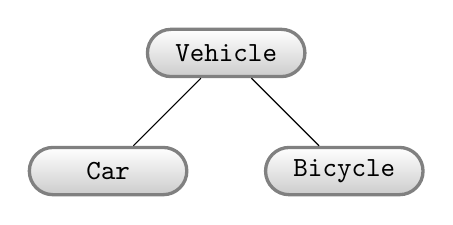
\begin{tikzpicture}[sibling distance=30mm,
    terminal/.style={
      % The shape:
      rectangle,minimum size=6mm,minimum width=20mm,rounded corners=3mm,
      % The rest
      very thick,draw=black!50,
      top color=white,bottom color=black!20,
      font=\ttfamily}]
    \node [terminal] {Vehicle} % root
    child { node [terminal] {Car} }
    child { node [terminal] {Bicycle} };
  \end{tikzpicture}
  \caption{Both a car and a bicycle is a (type of) vehicle.}
  \label{fig:inheritanceVehicle}
\end{figure}
%
Is-a relations can be implemented using class \idx{inheritance}, where vehicle is called the \idx{base class} and car and bicycle are each a \idx{derived class}. The advantage is that a derived class can inherent the members of the base class, \idx{override} and add possibly new members.

*******
%
\begin{verbatimwrite}{\ebnf/class.ebnf}
type <*classIdent*> ({*<*arg*>*}) [*as <*selfIdent*>*] 
  [*inherit <*baseClassIdent*>({*<*arg*>*})*]
  {*[*let <*binding*>*] |* [*do <*statement*>*]*}
  {*(*member |* abstract member |* default |* override*) <*memberDef*>*}
\end{verbatimwrite}
\syntax{\ebnf/class.ebnf}{A class definition with inheritance.}
%
The \lstinline[language=syntax]{<*classIdent*>} is the name of the class, \lstinline[language=syntax]{<*arg*>} are its optional arguments, \lstinline[language=syntax]{<*selfIdent*>} is an optional \idx{self identifier}, \lstinline[language=syntax]{<*baseClassIdent*>} is the name of another class that this class optionally builds upon using the \lstinline{inherit} keyword (see \Cref{sec:inheritance}), the optional \lstinline{let}-bindings and \lstinline{do}-statements define \idx{fields} and \idx{functions}, and \lstinline[language=syntax]{<*memberDef*>} are public members, i.e., \idx{properties} and \idx{methods}. Members may be regular members using the \lstinline{member} keyword or abstract members using either the \lstinline{abstract member}, 

************

Inheritance is indicated using the \lstinline[language=syntax]{inherit} keyword. \Cref{\ebnf/class.ebnf} shows the syntax for class definitions using inheritance, and an example of defining base and derived classes for vehicles is shown In \Cref{vehicle}.
%
%\fs{classInheritance}{New classes can be derived from old.}
\fs{vehicle}{New classes can be derived from old.}
%
In the example, a base class \lstinline{vehicle} is defined with members \lstinline{dir}, \lstinline{pos}, \lstinline{turn}, and \lstinline{forward}. The derived classes inherit all the members of the base class, but do not have access to any non-members of the base's constructor. I.e., \lstinline{car} and \lstinline{bicycle} automatically have methods \lstinline{turn} and \lstinline{forward}, and properties \lstinline{dir} and \lstinline{pos} with their accessors, but they do not have direct access to the fields \lstinline{p} and \lstinline{d}. Both derived classes additionally define a property \lstinline{wheels} and \lstinline{car} also define a method \lstinline{reverse}. Note that inheritance is one-way, and in spite that both derived classes define a member \lstinline{wheels}, the base class does not have a \lstinline{wheels} member.

Derived classes can replace base class members by defining new members \idx{overshadow} the base' member. The base' members are still available using the \idx[base@\lstinline{base}]{\keyword{base}}-keyword. Consider the example in the \Cref{memberOvershadowing}.
%
\fs{memberOvershadowing}{Inherited members can be overshadowed, but we can still access the base' member.}
%
In this case, we have defined two counters, each with an internal field \lstinline{i} and with members \lstinline{value} and \lstinline{inc}. The \lstinline{inc} method in \lstinline{counter} increments \lstinline{i} with 1, and in \lstinline{counter2} the field \lstinline{i} is incremented with 2. Note how \lstinline{counter2} inherits both members \lstinline{value} and \lstinline{inc}, but overshadows \lstinline{inc} by defining its own. Note also how \lstinline{counter2} defines another method \lstinline{incByOne} by accessing the inherited \lstinline{inc} method using the \keyword{base} keyword.

Even though derived classes are different from their base, the derived class includes the base class, which can be recalled using \idx[upcast]{upcasting} by the upcast operator \idx[:>@\lstinline{:>}]{\lexeme{:>}}. At compile-time this operator removes the additions and overshadowing of the derived class, as illustrated in \Cref{upCasting}. 
%
\fs{upCasting}{Objects can be upcasted resulting in an object as if it were its base. Implementations from the derived class are ignored.}
%
Here \lstinline{howdy} is derived from \lstinline{hello}, overshadows \lstinline{str}, and adds property \lstinline{altStr}. By upcasting object \lstinline{b}, we create object \lstinline{c} as a copy of \lstinline{b} with all its fields, functions, and members as if it had been of type \lstinline{hello}. I.e., \lstinline{c} contains the base class version of \lstinline{str} and does not have property \lstinline{altStr}. Objects \lstinline{a} and \lstinline{c} are now of same type and can be put into, e.g., an array as \lstinline{let arr = [|a, c|]}. Previously upcasted objects can also be downcasted again using the \idx{downcast} operator \idx[:?>@\lstinline{:?>}]{\keyword{:?>}}, but the validity of the operation is checked at runtime. Thus, \advice{avoid downcasting when possible.}

In the above, inheritance is used to modify and extend any class. I.e., the definition of the base classes were independent on the definitions of inherited classes. In that sense, the base classes were oblivious to any future derivation of them. Sometimes it is useful to define base classes, which are not independent on derived classes, and which impose design constraints on derived classes. Two such dependencies in F\# are abstract classes and interfaces to be described in the following sections.

\section{Abstract class}
\label{sec:abstract}
An \idx{abstract class} contains members defined using the \idx[abstract member@\lstinline{abstract member}]{\lstinline{abstract member}} and optionally the \idx[default@\lstinline{default}]{\lstinline{default}} keywords. An \lstinline{abstract member} in the base class is a type definition, and derived classes must provide an implementation using the \idx[override@\lstinline{override}]{\keyword{override}} keyword. Optionally, the base class may provide a default implementation using the \lstinline{default} keyword, in which case overriding is not required in derived classes. Objects of classes containing abstract members without default implementations cannot be instantiated, but derived classes that provide the missing implementations can be. Note that abstract classes must be given the \idx[AbstractClass@\lstinline{[<AbstractClass>]}]{\lstinline{[<AbstractClass>]}} attribute. Note also that in contrast to overshadowing, upcasting keeps the implementations of the derived classes. Examples of this are shown in \Cref{abstractClass}.
%
\fs{abstractClass}{In contrast to regular objects, upcasted derived object use the derived implementation of abstract methods.}
%
In the example, we define a base class and two derived classes. Note how the abstract member is defined in the base class using the \lexeme{:}-operator as a type declaration rather than a name binding. Note also that since the base class does not provide a default implementation, the derived classes supply an implementation using the \keyword{override}-keyword. In the example, objects of \lstinline{baseClass} cannot be created, since such objects would have no implementation for \lstinline{this.hello}. Finally, the two different derived and upcasted objects can be put in the same array, and when calling their implementation of \lstinline{this.hello} we still get the derived implementations, which is in contrast to overshadowing.

Abstract classes may also specify a default implementation, such that derived classes have the option of implementing an overriding member, but are not forced to. In spite that implementations are available in the abstract class, the abstract class still cannot be used to instantiate objects. Such a variant is shown in \Cref{abstractDefaultClass}.
%
\fs[linebackgroundcolor={%
\highlightRange{\getrefnumber{abstractDefaultClassStart}}{\getrefnumber{abstractDefaultClassEnd}}%
}]{abstractDefaultClass}{Default implementations in abstract classes makes implementations in derived classes optional. Compare with \Cref{abstractClass}.}%
%
In the example, the program in \Cref{abstractClass} has been modified such that \lstinline{greeting} is given a default implementation for \lstinline{str}, in which case, \lstinline{hello} does not need to supply one. However, in order for \lstinline{howdy} to provide a different greeting, it still needs provide an override member. 

Note that even if all abstract members in an abstract class has defaults, objects of its type can still not be created, but must be derived as, e.g., shown with \lstinline{hello} above.

As a side note, every class implicitly derives from a base class \idx[System.Object@\lstinline{System.Object}]{\lstinline{System.Object}} which, which is an abstract class defining among other members the \lstinline{ToString} method with default implementation.

\section{Interfaces}
\label{sec:interfaces}
Inheritance of an abstract base class allows an application to rely on the definition of the base regardless of any future derived classes. This gives great flexibility, but at times even less knowledge is needed about objects in order to write useful applications. This is what \idx[interface]{interfaces} offer. An interface specifies which members must exist but nothing more. Interfaces are defined as an abstract class \emph{without arguments} and \emph{only with abstract members}. Classes implementing interfaces must specify implementations for the abstract members using the \idx[interface with@\lstinline{interface with}]{\lstinline{interface with}} keywords. Objects of classes implementing interfaces can be upcasted as if they had an abstract base class of the interface' name. Consider the example in \Cref{classInterface}.
%
\fs{classInterface}{Interfaces specifies which members classes contain, and with upcasting gives more flexibility than abstract classes.}
%
Here, two distinctly different classes are defined: \lstinline{house} and \lstinline{person}. These are not related by inheritance since no sensible common structure seems available. However, they share structures in the sense that they both have an integer property and a \lstinline{float -> float} method. For each of the derived classes, these members have different meanings. Still, some treatment of these members by an application will only rely on their type and not their meaning. E.g., in \Cref{classInterface} the \lstinline{printfn} function only needs to know the member's type not their meaning. As a consequence, the application can upcast them both to the implicit abstract base class \lstinline{IValue}, put them in an array, and apply a function using the member definition of \lstinline{IValue} with the higher-order \lstinline{List.iter} function. Another example could be a higher-order function calculating average values: For average values of the number of floors and average value of the length of people's names, the higher-order function would only need to know that both of these classes implements the \lstinline{IValue} interfaces in order to calculate the average of list of either objects types.

As a final note, inheritance ties classes together in a class hierarchy. Abstract members enforce inheritance and impose constraints on the derived classes. Like abstract classes, interfaces impose constraints on derived classes, but without requiring a hierarchical structure.

\section{Programming intermezzo: Chess}
To demonstrate the use of hierarchies, consider the following problem
\begin{problem}
  The game of chess is a turn-based game for two, which consists of a board of $8\times 8$ squares and a set of 16 black and 16 white pieces. A piece can be either a king, queen, rook, bishop, knight or pawn and each piece has a specific movement pattern on the board. Pieces are added to, moved on, and removed from the board during the game, and there can be at most one piece per square. A piece strikes another piece of opposing color by moving to its square and the piece of opposing color is removed from the game. The game starts with the configuration shown in \Cref{fig:chessNewGame}.\\[\parskip]

  Make a program that allows two humans to play simple chess using only kings and rooks. The king must be able to move to all neighboring squares not occupied by a piece of the same color and cannot move onto a square, where it can be struck in the next turn. The rook must be able to move in horizontal and vertical lines until a piece of the same color or up to and including a piece of opposing color. Make a program that allows two humans to play simple chess.
\end{problem}
\begin{figure}
  \centering
  \newgame
  \showboard
  \caption{Starting position for the game of chess.}
  \label{fig:chessNewGame}
\end{figure}
Since we expect that the solution to the above problem is going to be a relatively long program, we have decided to split the code into a library and an application program. Before writing a library, it is often useful to start thinking about how the library should be used. Thus we start by sketching the application program, and in the process consider options for the main methods and properties to be used.

We also foresee future extensions to include more pieces, but also that these pieces will obey the same game mechanics that we design for the present problem. Thus, we will put the main part of the library in a file defining the module called \lstinline{Chess} and the derived pieces in another file defining the module \lstinline{Pieces}.

%For a solution, the application must be able to create pieces of various types and colors, to set, move and remove pieces position, and to acquire a piece's location on the board, if it is still in the game. 
%
Every game needs a board, and we will define a class \lstinline{Board}. A board is like an array, so it seems useful to be able to move pieces by index notation. Thus, the board must have a two-dimensional \lstinline{Item} property. We also decide that each position will hold an option type such when a square is empty it holds \lstinline{None} otherwise it holds piece \lstinline{p} as \lstinline{Some p}. Although chess notation would be neat, for ease of programming we will let index (0,0) correspond to position a1 in chess notation etc. The most common operation will probably be to move pieces around, so we will give the board a \lstinline{move} method. We will most likely also like to print the board with pieces in their right locations. For simplicity we choose to override the \lstinline{ToString} method in \lstinline{Board}, and that this method also prints information about each individual piece such as where it is, where it can move to, and which pieces it can either protect or hit. The pieces that a piece can protect or hit we will call the piece' neighbor pieces.

A piece can be one of several types, so this gives a natural hierarchical structure, which is well suited for inheritance, Each piece must be given a color, which may conveniently be given as argument at instantiation. Thus, we have decided to make a base class called \lstinline{chessPiece} with argument \lstinline{Color}, and derived classes \lstinline{king} and \lstinline{rook}. The color may conveniently define as a discriminated union type of either \lstinline{White} or \lstinline{Black}. Each piece will also override the \lstinline{ToString} method for ease of printing. The override will be used in conjunction with the board's override, so it should only give information about the piece' type and color. For compact printing, we will use a single letter for the type of piece, upper case if white, and lower case if black. We expect the pieces also to need to know something about the relation to board, so we will make a \lstinline{position} property, which holds the coordinates of the piece, and we will make a \lstinline{availableMoves} method that lists the possible moves, a piece can make. Thus, we produce the application in \Cref{chessAppCode}, and an illustration of what the program should do is shown in \Cref{fig:chessKingsGame}.
%
\fsCode{chessApp}{chessAppCode}{A chess application.}{}
%
\begin{figure}
  \centering
  \newgame
  \loadgame{figures/kingsGame}
  \showboard
  \hspace*{1cm}
  \loadgame{figures/kingsGameMove}
  \showboard
  \caption{Starting at the left and moving white rook to b4.}
  \label{fig:chessKingsGame}
\end{figure}
At this point, we are fairly happy with the way the application is written. The double bookkeeping of pieces in an array and on the board seems a bit excessive, but for testing, it seems useful to be able to easily access all pieces both those in play and struck. Although the \lstinline{position} property of a \lstinline{chessPiece} could be replaced by a function searching for a specific piece on the board, we have a hunch that we will need to retrieve a piece' position often, and that this double will most likely save execution time later. 

Continuing our outer to inner approach, as a second step, we consider the specific pieces: They will inherit a base piece and implement the details that are special for that piece. Each piece is signified by its color and its type, and each type has a specific motion pattern. Since we have already decided to use discriminated unions for the color, it seems natural to let the color be part of the constructor of the base class. As in the example application in \Cref{chessAppCode}, pieces are upcasted to \lstinline{chessPiece}, then the base class must know how to print the piece type. For this, we will define an abstract property, such that everything needed for overriding \lstinline{ToString} is available to the base class, but also such that the name of the type of the piece is set in the derived class.

For a piece on the board, its available moves depend on its type and the other pieces. The application program will need to make a decision on whether to move the piece depending on which vacant squares, it can move to, and its relation to its neighbors, i.e., is the piece protecting one of its own color, or does it have the opportunity to hit an opponent. Thus given the board with all the pieces, it seems useful that \lstinline{availableMoves} returns two lists: a list of vacant squares and a list of neighboring pieces of either color. Each piece has certain movement pattern, which we will specify regardless of the piece' position on the board and relation to other pieces. Thus, this will be an abstract member called \lstinline{candiateRelativeMoves} implemented in the derived pieces. These candidate relative moves are then to be sifted for legal moves, and the process will be the same for all pieces, which thus can be implemented in the base class as the \lstinline{availableMoves}.

Many pieces move in runs, e.g., the rook can move horizontally and vertically until there is another piece. Vacant squares behind the blocking piece are unavailable. For a rook, we thus must analyze four runs: northward, eastward, southward, and westward. For each run, we must consult the board to see, how many vacant fields there are in that direction, and which is the piece blocking if any. Thus, we decide that the board must have a function that can analyze a list of runs and that the result is concatenated into a single list of vacant squares and a single list of neighboring pieces if any. This function we call \lstinline{getVacentNNeighbours}. And so we arrive at \Cref{pieces}.
%
\fsImplementation{pieces}{pieces}{An extension of chess base.}{}
%
The king has the simplest relative movement candidates being the hypothetical eight neighboring squares. For rooks, the relative movement candidates are somewhat more complicated. For rooks, we would like to use \lstinline{List.map} to convert a list of single indices into double indices to calculate each run. And we have gathered all the elemental functions for this in \lstinline{indToRel}. E.g., function at index 0, we may write \lstinline{List.map indToRel.[0] indices}. However, we would also like to use \lstinline{List.map} to perform this operation for all elemental functions in \lstinline{indToRel}. Direct joining such two applications of \lstinline{List.map} does not work, since \lstinline{List.map} takes a function and a list as its arguments, and for the second application, these two arguments should switch order.  I.e., the first time it is \lstinline{indices} that takes the role of the list, while the second it is \lstinline{indToRel} that takes the role of the list. A standard solution in functional programming is to use currying and the \idx{\lstinline{swap}} function as illustrated in line~\ref{chessPieceSwapApp}: The function is equivalent to the anonymous function \lstinline{fun elm -> swap List.map indices elm}, and since \lstinline{swap} swaps the arguments of a function, this reduces to \lstinline{fun elm -> List.map elm indices}, which is exactly what is needed.

The final step will be to design the \lstinline{Board} and \lstinline{chessPiece} classes. The Chess module implements discriminated unions for color and an integer tuple for a position. These are shown in \Cref{chessDiscriminatedUniont}.
%
\fsImplementation{chess}{chessDiscriminatedUniont}{A chess base: Module header and discriminated union types.}{lastline=3}
%
The \lstinline{chessPiece} will need to know what a board is, so we must define it as a mutually recursive class with \lstinline{Board}. Further, since all pieces must supply an implementation of \lstinline{availableMoves}, we set it to be abstract by the abstract class attribute and with an abstract member. The board will need to be able to ask for a string describing each piece and to keep the board on the screen we include an abbreviated description of the piece's properties color and piece type. The result is shown in \Cref{chessPiece}.
%
\fsImplementation{chess}{chessPiece}{A chess base. Abstract type chessPiece.}{firstnumber=4,firstline=4,lastline=24} % Absolute reference!
%

Our \lstinline{Board} class is by far the largest and will be discussed by \Crefrange{chessBoardConstructor}{chessBoardgetVacantNOccupied}. The constructor is shown in \Cref{chessBoardConstructor}.
%
\fsImplementation{chess}{chessBoardConstructor}{A chess base: the constructor}{firstnumber=25,firstline=25,lastline=42} % Absolute reference!
%
For memory efficiency, the board has been implemented using a \lstinline{Array2D}, since pieces will move around often. For later use in the members shown in \Cref{chessBoardgetVacantNOccupied} we define tow functions that converts relative coordinates into absolute coordinates on the board, and removes those that fall outside the board. These are called \lstinline{validPositionWrap} and \lstinline{relativeToAbsolute}.

For ease of use in an application, \lstinline{Board} implements \lstinline{Item}, such that the board can be read and writing to using array notation. And \lstinline{ToString} is overridden, such that an application may print the board anytime using a \lstinline{printf} function. This is shown in \Cref{chessBoardItem}.
%
\fsImplementation{chess}{chessBoardItem}{A chess base: Board header, constructor, and non-static members.}{firstnumber=43,firstline=43,lastline=73} % Absolute reference!
%
Note that for efficiency, location is also stored in each piece, so \lstinline{set} also needs to update the particular piece' position as done in line~\ref{chessItemSet}. Note also that the board is printed with the first coordinate of the board being rows and second columns and such that element (0,0) is at the bottom right complying with standard chess notation.

The main computations are done in the static methods of the board as shown in \Cref{chessBoardgetVacantNOccupied}. 
%
\fsImplementation{chess}{chessBoardgetVacantNOccupied}{A chess base: Board static members.}{firstnumber=74,firstline=74} % Absolute reference!
%
A chess piece must implement \lstinline{candiateRelativeMoves}, and we decided in \Cref{chessPiece} that moves should be specified relative to the piece' position. Since the piece does not know, which other pieces are on the board, it can only specify all potential positions. For convenience, we will allow pieces to also specify positions outside the board, such that, e.g., the rook can specify the 7 nearest neighboring squares up, down, left, and right regardless that some may be outside the board. Thus \lstinline{getVacantNNeighbours} must first convert the relative positions to absolute and clip any outside the board. This is done by \lstinline{relativeToAbsolute}. Then for each run, the first occupied square must be identified. Since \lstinline{availableMoves} must return two lists, vacant squares, and immediate neighbors, this structure is imposed on the output of \lstinline{convertNWrap} as well. This is computed in \lstinline{getVacantNOccupied} by use of the built-in \lstinline{List.findIndex} function. This function returns the index of the first element in a list for which the supplied function is true and otherwise throws an exception. Exceptions are always somewhat inelegant, but in this case, it is harmless, since the exception signifies a valid situation where no pieces exist on the run. After having analyzed all runs independently, then all the vacant lists are merged and all the neighboring pieces are merge and both are returned to the caller.

Compiling the library files with the application and executing gives the result shown in \Cref{chessApp}.
%
\fsOutput{chessApp}{Running the program. Compare with \Cref{fig:chessKingsGame}.}{}
%
We see that the program has correctly determined that initially, the white king has the white rook as its neighbor and due to its location in the corner only has two free positions to move to. The white rook has many and the black king as its neighbor. The black king is free to move to all its eight neighboring fields. After moving the white rook to (3,1) or b4 in regular chess notation, then the white king has no neighbors, the white rook and the black king are now neighbors with an appropriate restriction on their respective vacant squares. These simple use-tests are in no way a thorough test of the quality of the code, but they give us a good indication that our library offers a tolerable interface for the application, and that at least major parts of the code function as expected. Thus, we conclude this intermezzo.

%%% Local Variables:
%%% TeX-master: "fsharpNotes"
%%% End:



\documentclass[fsharpnotes.tex]{subfiles}

\begin{document}
\chapter{The Object-Oriented Programming Paradigm}
\label{chap:oopp}
\idx{Object-oriented programming} is a paradigm for encapsulating data and methods into cohesive units. Key features of object-oriented programming are:
\begin{description}
\item[Encapsulation]~\\
Data and methods are collected into a cohesive unit, and an application program need only focus on how to use the object, not on its implementation details.
\item[Inheritance]~\\
Objects are organized in a hierarchy of gradually increased specialty. This promotes a design of code that is of general use, and code reuse.
\item[Polymorphism]~\\
By overriding methods from a base class, derived classes define new data types while their methods still produce results compatible with the base class definitions.
\end{description}

Object-oriented programming has a well-developed methodology for analysis and design. The analysis serves as input to the design phase, where the analysis reveals \idx{what} a program is supposed to do, and the design \idx{how} it is supposed to be doing it. The analysis should be expressed in general terms irrespective of the technologic constraints, while the design should include technological constraints such as defined by the targeted language and hardware.

The primary steps for \idx{object-oriented analysis and design} are:
\begin{enumerate}
\item identify objects,\label{item:analysis}\label{item:identifyObjects}
\item describe object behavior, \label{item:objectBehaviour}
\item describe object interactions, \label{item:objectInteraction}
\item describe some details of the object's inner workings,\label{item:design}\label{item:objectDetails}
\item write a precise description for classes, properties and methods using, e.g., F\#'s XML documentation standard,
\item write mockup code,  \label{item:objectMockup}
\item write unit tests and test the basic framework using the mockup code,\label{item:implementation}
\item replace the mockup with real code while testing to keep track of
  your progress. Extend the unit test as needed,
\item evaluate code in relation to the desired goal,
\item complete your documentation both in-code and outside.
\end{enumerate}
Steps~\ref{item:analysis}--\ref{item:design} are the analysis phase which gradually stops in step~\ref{item:design}, while the design phase gradually starts at step~\ref{item:design} and gradually stops when actual code is written in step~\ref{item:implementation}. Notice that the last steps are identical to imperative programming, \Cref{chap:imperative}. Programming is never a linear experience, and you will often need to go back to previous steps to update or change decisions. You should not refrain from improving your program design and implementation, but you should always be mindful of the goal. Often less than the perfect solution will suffice.

An object-oriented analysis can be a daunting process. A good starting point is a \idx{use case}, \idx{problem statement}, or a \idx{user story}, which in human language describes a number of possibly hypothetical interactions between a user and a system with the purpose of solving some task. Two useful methodologies for performing an object-oriented analysis is the method of nouns-and-verbs and the unified modeling language, described in the following sections.

\section{Identification of Objects, Behaviors, and Interactions by Nouns-and-Verbs}
A key point in object-oriented programming is that objects should to a large extent be independent and reusable. As an example, the type \lstinline|int| models the concept of integer numbers. It can hold integer values from -2,147,483,648 to 2,147,483,647, and a number of standard operations and functions are defined for it. We may use integers in many different programs, and it is certain that the original designers did not foresee our use, but strived to make a general type applicable for many uses. Such a design is a useful goal when designing objects, that is, our objects should model the general concepts and be applicable in future uses. 

Analyzing a specific use-case, good candidates for objects are persons, places, things, events, concept etc., which are almost always characterized by being \idx{nouns} in the text. Interactions between objects are actions that bind objects together, and actions are often associated with \idx{verbs}. When choosing methods, it is important to maintain an object-centered perspective, i.e., for a general-purpose object, we should limit the need for including information about other objects. E.g., a value of type \lstinline|int| need not know anything about the program in which it is being used.

Said briefly, the \idx{nouns-and-verbs method} is:
%
\begin{quote}
  Nouns are object candidates, and verbs are candidate methods that describe interactions between objects.
\end{quote}
%

\section{Class Diagrams in the Unified Modelling Language}
Having found an initial list of candidate objects and interactions, it is often useful to make a drawing of these relations with an increased focus on the object's inner workings. A \idx{class diagram} is a schematic drawing of the program, highlighting its object-oriented structure, and we will use the \idx{Unified Modelling Language 2} (\idx{UML}) \cite{uml2} standard. The standard is very broad, and here we will discuss structure diagrams for use in describing objects. 

A class is drawn as shown in \Cref{fig:class}.
\begin{figure}
  \centering
  \begin{tikzpicture}
    \begin{class}[text width=9cm]{ClassName}{0,0}
      \attribute{value-identifier : type}
      \attribute{value-identifier : type = default value}
      \operation{function-identifier (arg : type) (arg : type) ... : type}
      % virtual operation
      \operation[0]{function-identifier (arg : type) (arg : type) ... : type}
    \end{class}
    \end{tikzpicture}
  \caption{A UML diagram for a class consists of it's name, zero or more attributes, and zero or more methods.}
  \label{fig:class}
\end{figure}
In UML, classes are represented as boxes with their class name. Depending on the desired level of details, zero or more properties and methods are described. These describe the basic interface to the class and objects of its type. Abstract members that require an implementation are shown in cursive. Here we have used F\# syntax to conform with this book theme, but typically C\# syntax is used.
%
\begin{comment}
\begin{figure}
  \centering
  \begin{tikzpicture}%[show background grid] 
    \begin{class}[text width=7cm]{Class}{0,0} \attribute{+ Public}
      \attribute{\# Protected}
      \attribute{- Private}
      \attribute{$\sim$ Package} 
    \end{class}
    \begin{class}[text width=7cm]{BankAccount}{0,-3} \attribute{+ owner : String}
      \attribute{+ balance : Dollars}
      \operation{+ deposit( amount : Dollars )} \operation{+ withdrawal( amount : Dollars )} \operation{\# updateBalance( newBalance : Dollars
        )} 
    \end{class}
  \end{tikzpicture}
  \caption{visibility}
  \label{fig:visibility}
\end{figure}
\begin{figure}
  \centering
  \begin{tikzpicture}
    \begin{abstractclass}[text width=5cm]{BankAccount
      }{0 ,0}
      \attribute{owner : String}
      \attribute{balance : Dollars = 0}
      \operation{deposit(amount : Dollars)} \operation[0]{withdrawl(amount : Dollars)}
    \end{abstractclass} 
  \end{tikzpicture}
  \caption{abstract class}
  \label{fig:abstractClass}
\end{figure}
\end{comment}
%
Interfaces are a special type of class that require an implementation. To highlight this, UML uses the notation shown in \Cref{fig:interface}.\jon{Add programming examples for each of these UML structures}
\begin{figure}
  \centering
  \begin{tikzpicture}%[show background grid] 
    \begin{interface}[text width=9cm]{InterfaceName}{0,0}
      \attribute{value-identifier : type}
      \attribute{value-identifier : type = default value}
      \operation{function-identifier (arg : type) (arg : type) ... : type}
    \end{interface} 
  \end{tikzpicture}
  \caption{An interface is a class that requires an implementation.}
  \label{fig:interface}
\end{figure}

 
Relations between classes and objects are indicated by lines and arrows. The most common ones are summarized in \Cref{fig:arrows}.
\begin{figure}
  \centering
  \fbox{
    \begin{tikzpicture}
      % \draw[umlcd style dashed line] (0,4) --(8,4);
      % \draw[splitline] (0,3) --(8,3);
      \node [left] at (-2,5) {Associate:};
      \node (associateLeft) [left] at (0,5) {HostA};
      \node (associateRight) [right] at (8,5) {HostB};
      \association{associateLeft}{objectsAinB}{0..1}{associateRight}{objectsBinA}{0..*} ;
      
      \node [left] at (-2,4) {\parbox[r]{2.5cm}{\raggedleft Unidirectional associate:}};
      \node (uniAssociateLeft) [left] at (0,4) {Host};
      \node (uniAssociateRight) [right] at (8,4) {Guest};
      \unidirectionalAssociation{uniAssociateLeft}{guestObj}{0..*}{uniAssociateRight};

      \node [left] at (-2,3) {Aggregate:};
      \node (aggregateLeft) [left] at (0,3) {Host};
      \node (aggregateRight) [right] at (8,3) {Guest};
      \aggregation{aggregateLeft}{guestObj}{4}{aggregateRight};
      
      \node [left] at (-2,2) {Compose:};
      \node (composeLeft) [left] at (0,2) {Owner};
      \node (composeRight) [right] at (8,2) {Dependent};
      \composition{composeLeft}{depObj}{1..*}{composeRight};
      
      \node [left] at (-2,1) {Implement:};
      \node (interfaceDerived) [left] at (0,1) {Derived};
      \node (interfaceBase) [right] at (8,1) {Interface};
      \draw[umlcd style implement line] (interfaceBase) -- (interfaceDerived);
      
      \node [left] at (-2,0) {Inherit:};
      \node (inheritDerived) [left] at (0,0) {Derived};
      \node (inheritBase) [right] at (8,0) {Base};
      \draw[umlcd style inherit line] (inheritBase) -- (inheritDerived);
    \end{tikzpicture}
  }
  \caption{Arrows used in class diagrams to show relations between objects.}
  \label{fig:arrows}
\end{figure}
Their meaning will be described in detail in the following. 


\subsection{Associations}
A family of relations is association, aggregation, and composition, and these are distinguished by how they handle the objects they are in relation with. The relation between the three relations is shown in \Cref{fig:associationAggregationCompositionRelation}.
\begin{figure}
  \centering
  \includegraphics[width=0.45\textwidth]{associationAggregationComposition}
  \caption{The relation between Association, Aggregation and Composition in UML.}
  \label{fig:associationAggregationCompositionRelation}
\end{figure}
Aggregational and compositional are specialized types of associations that imply ownership and are often called \idx[has-a relation]{has-a} relations. A composition is a collection of parts that makes up a whole. In object-oriented design, a compositional relation is a strong relation, where a guest object makes little sense without the host, as a room cannot exist without a house. An aggregation is a collection of assorted items, and in object-oriented design, an aggregational relation is a loose relation, like how a battery can meaningfully be separated from a torchlight. Some associations are neither aggregational nor compositional, and commonly just called an association. An association is a group of people or things linked for some common purpose a cooccurrence. In object-oriented design, associations between objects are the loosest possible relations, like how a student may be associated with the local coffee shop. Sometimes associational relations are called a  \idx[knows-about relation]{knows-about}.

\paragraph{Association}\idxs{association}~\\
The most general type of association, which is just called an association, is the possibility for objects to send messages to each other. This implies that one class knows about the other, e.g., uses it as arguments of a function or similar. A host is associated with a guest if the host has a reference to the guest. Objects are reference types, and therefore, any object which is not created by the host, but where a name is bound to a guest object but not explicitly copied, then this is an association relation.

Bidirectional association means that classes know about each other. The UML notation is shown in \Cref{fig:association}.
\begin{figure}
  \centering
  \begin{tikzpicture}
    \begin{class}{HostA}{0,0}
    \end{class}
    \begin{class}{HostB}{11,0}
    \end{class} 
    \association{HostA}{objectsAinB}{0..1}{HostB}{objectsBinA}{0..*}
  \end{tikzpicture}
  \caption{Bidirectional association is shown as a line with optional annotation.}
  \label{fig:association}
\end{figure}
Association may be annotated by an identifier and a multiplicity. In the figure, HostA has 0 or more variables of type HostB named objectsBinA, while HostB has 0 or 1 variables of HostA named objectsAinB. The multiplicity notation is very similar to F\#'s slicing notation. Typical values are shown in \Cref{tab:multiplicity}.
\begin{table}
  \centering
  \begin{tabular}{|l|l|}
    \hline
    n & exactly n instances\\
    * & zero or more instances \\
    n..m & n to m instances\\
    n..* & from n to infinite instances\\
    \hline
  \end{tabular}
  \caption{Notation for association multiplicities is similar to F\#'s slicing notation.}
  \label{tab:multiplicity}
\end{table}
If the association is unidirectional, then an arrow is added for emphasis, as shown in \Cref{fig:unidirectionalAssociation}.
\begin{figure}
  \centering
  \begin{tikzpicture}
    % \draw[help lines] (-7,-6) grid (6,0);
    \begin{class}{Host}{0,0}
    \end{class}
    \begin{class}{Guest}{9,0}
    \end{class}
    \unidirectionalAssociation{Host}{guestObj}{1}{Guest}
  \end{tikzpicture}  
  \caption{Unidirectional association shows a one-side \emph{has-a} relation.}
  \label{fig:unidirectionalAssociation}
\end{figure}
In this example, Host knows about Guest and has one instance of it, and Guest is oblivious about Host.

A programming example showing a unidirectional association is given in \Cref{umlAssociation}.
% 
\fsCode{umlAssociation}{umlAssociation}{The \lstinline{student} is associated with a \lstinline{teacher}.}{}
% 
Here, the \lstinline{student} is unidirectionally associated with a \lstinline{teacher} since the \lstinline{student} can send and receive messages to and from the \lstinline{teacher}. The \lstinline{teacher}, on the other hand, does not know anything about the \lstinline{student}. In UML this is depicted as shown in \Cref{fig:umlAssociationUML}.
\begin{figure}
  \centering
  \begin{tikzpicture}
    \begin{class}{student}{0,0}
    \end{class}
    \begin{class}{teacher}{9,0}
    \end{class} 
    \unidirectionalAssociation{student}{}{}{teacher}
  \end{tikzpicture}
  \caption{The \lstinline{teacher} and \lstinline{student} objects can access each other's functions, and thus they have an association relation.}
  \label{fig:umlAssociationUML}
\end{figure}

\paragraph{Aggregation}\idxs{aggregation}~\\
Aggregated relationships are a specialization of associations. As an example, an author may have written a book, but once created, the book gets a life independent of the author and may, for example, be given to a reader, and the book continues to exist even when the author dies. That is, In aggregated relations, the host object has a reference to a guest object and may have created the guest, but the guest will be shared with other objects, and when the host is deleted, the guest is not.

Aggregation is illustrated using a diamond tail and an open arrow, as shown in \Cref{fig:aggregation}.
\begin{figure}
  \centering
  \begin{tikzpicture}
    \begin{class}{Host}{0,0}
    \end{class}
    \begin{class}{Guest}{9,0} 
    \end{class}
    \aggregation{Host}{guestObj}{4}{Guest}
  \end{tikzpicture}
  \caption{Aggregation relations are a subset of associations where local aliases are stored for later use.}
  \label{fig:aggregation}
\end{figure}
Here the Host class has stored aliases to four different Guest objects.

An programming example of an aggregation relation is given in \Cref{umlAggregation}.
% 
\fsCode{umlAggregation}{umlAggregation}{The \lstinline{book} has an aggregated relation to \lstinline{author} and \lstinline{reader}.}{}
% 
In aggregated relations, there is a sense of ownership, and in the example, the \lstinline{author} object creates a \lstinline{book} object which is published and bought by a reader. Hence the \lstinline{book} change ownership during the execution of the program. In UML this is to be depicted as shown in \Cref{fig:umlAggregationUML}.
\begin{figure}
  \centering
  \begin{tikzpicture}
    \begin{class}{author}{0,0}
    \end{class}
    \begin{class}{reader}{9,0} 
    \end{class}
    \begin{class}{book}{4.5,2}
    \end{class}
    \aggregation{author}{}{}{book}
    \aggregation{reader}{}{}{book}
  \end{tikzpicture}
  \caption{A book is an object that can be owned by both an author and a reader.}
  \label{fig:umlAggregationUML}
\end{figure}

\paragraph{Composition}\idxs{composition}~\\
A compositional relationship is a specialization of aggregations. As an example, a dog has legs, and dog legs can not very sensibly be given to other animals. That is, in compositional relations, the host creates the guest, and when the host is deleted, so is the guest.  A composition is a stronger relation than aggregation and is illustated using a filled filled diamond tail, as illustrated in \Cref{fig:composition}.
\begin{figure}
  \centering
  \begin{tikzpicture}
    \begin{class}{Owner}{0,0} 
    \end{class}
    \begin{class}{Dependent}{9,0}
    \end{class}
    \composition{Owner}{depObj}{1..*}{Dependent}
  \end{tikzpicture}
  \caption{Composition relations are a subset of aggregation where the host controls the lifetime of the guest objects.}
  \label{fig:composition}
\end{figure}
In this example, Owner has created 1 or more objects of type Dependent, and when Owner is deleted, so are these objects.

A programming example of a composition relation is given in \Cref{umlComposition}.
% 
\fsCode{umlComposition}{umlComposition}{The \lstinline{dog} object is a composition of four \lstinline{leg} objects.}{}
% 
In \Cref{umlComposition}, a \lstinline{dog} object creates four \lstinline{leg} objects, and it makes less sense to be able to turn over the ownership of each \lstinline{leg} to other objects. Thus, a \lstinline{dog} is a composition of \lstinline{leg} objects. Using UML, this should be depicted as shown in \Cref{fig:umlCompositionUML}.
\begin{figure}
  \centering
  \begin{tikzpicture}
    \begin{class}{dog}{0,0} 
    \end{class}
    \begin{class}{leg}{9,0}
    \end{class}
    \composition{dog}{}{}{leg}
  \end{tikzpicture}
  \caption{A dog is a composition of legs.}
  \label{fig:umlCompositionUML}
\end{figure}

\subsection{Inheritance-type relations}
Classes may inherit\idxs{inheritance} other classes where the parent is called the base class and the children its derived classes. Such a relation is often called an \idx[is-a relation]{is-a} relation, since the derived class \emph{is a} kind of base class.

\paragraph{Inheritance}
Inheritance is a relation between properties of classes. As an example, a student and a teacher is a type of person. All persons have names, while a student also has a reading list, and a teacher also has a a set of slides. Thus, both students and teacher may inherit from a person to gain the common property, name. In UML this is illustated with an non-filled, closed arrow as shown in \Cref{fig:inherit}.
\begin{figure}
  \centering
  \begin{tikzpicture}
    \begin{class}[text width=5cm]{BaseClassName}{0,0}
    \end{class}
    \begin{class}[text width=5cm]{DerivedClassA}{-3,-2}
      \inherit{BaseClassName}
    \end{class}
    \begin{class}[text width=5cm]{DerivedClassB}{3,-2} 
      \inherit{BaseClassName} 
    \end{class}
  \end{tikzpicture}
  \caption{Inheritance is shown by a closed arrowhead pointing to the base.}
  \label{fig:inherit}
\end{figure}
Here two classes inherit the base class.

A programming example of an inheritance is given in \Cref{umlInheritance}.
% 
\fsCode{umlInheritance}{umlInheritance}{The \lstinline{student} and the \lstinline{teacher} class inherits from the \lstinline{person} class.}{}
% 
In \Cref{umlInheritance}, the \lstinline{student} and the \lstinline{teacher} classes are derived from the same \lstinline{person} class. Thus, they all three have the \lstinline{name} property. Using UML, this should be depicted as shown in \Cref{fig:umlInheritanceUML}.
\begin{figure}
  \centering
  \begin{tikzpicture}
    \begin{class}{person}{4.5,2}
    \end{class}
    \begin{class}{student}{0,0}
      \inherit{person}
    \end{class}
    \begin{class}{teacher}{9,0} 
      \inherit{person}
    \end{class}
  \end{tikzpicture}
  \caption{A student and a teacher inherit from a person class.}
  \label{fig:umlInheritanceUML}
\end{figure}

\paragraph{Interface}
An interface is a relation between the properties of an abstract class and a regular class. As an example, a television and a car both have buttons, that you can press, although their effect will be quite different. Thus, a television and a car may both implement the same interface. In UML, interfaces are shown similarly to inheritance, but using a stippled line, as shown in \Cref{fig:implement}.
\begin{figure}
  \centering
  \begin{tikzpicture}
    \begin{interface}[text width=5cm]{InterfaceName}{0,0} 
    \end{interface}
    \begin{class}[text width=5cm]{DerivedClassA}{-3,-2}
      \implement{InterfaceName}
    \end{class}
    \begin{class}[text width=5cm]{DerivedClassB}{3,-2} 
      \implement{InterfaceName} 
    \end{class}
  \end{tikzpicture}
  \caption{Implementations of interfaces is shown with stippled line and closed arrowhead pointing to the base.}
  \label{fig:implement}
\end{figure}

A programming example of an interface is given in \Cref{umlInterface}.
% 
\fsCode{umlInterface}{umlInterface}{The \lstinline{television} and the \lstinline{car} class both implement the \lstinline{button} interface.}{}
% 
In \Cref{umlInterface}, the \lstinline{television} and the \lstinline{car} classes implement the \lstinline{button} interface. Hence, although they are different classes, they both have the \lstinline{press ()} method and, e.g., can be given as a function requiring only the existence of the \lstinline{press ()} method. Using UML, this should be depicted as shown in \Cref{fig:umlInterfaceUML}.
\begin{figure}
  \centering
  \begin{tikzpicture}
    \begin{class}{button}{4.5,2}
    \end{class}
    \begin{class}{television}{0,0}
      \implement{button}
    \end{class}
    \begin{class}{car}{9,0} 
      \implement{button}
    \end{class}
  \end{tikzpicture}
  \caption{A student and a teacher inherit from a person class.}
  \label{fig:umlInterfaceUML}
\end{figure}

\subsection{Packages}
\paragraph{Namespace and modules}
For visual flair, modules and namespaces are often visualized as \idx[package]{packages}, as shown in \Cref{fig:package}. A package is like a module in F\#.
\begin{figure}
  \centering
  \begin{tikzpicture} 
    \begin{package}{APackageName}
      \begin{class}[text width=3cm]{Base}{0,0} 
        \attribute{aValue : int = 0}
        \operation{get:  () -> int }
        \operation[0]{set: int -> ()} 
      \end{class}
      \begin{class}[text width=4cm]{Guest}{-4,-4}
        \attribute{aString : string}
        \operation{writeMessage : () -> ()}
      \end{class}
      \begin{class}[text width=6cm]{Derived}{4, -4}
        \inherit{Base} 
        \attribute{dictionary : string list}
        \operation{checkSpelling : string -> bool}
        \operation{set : int -> ()} 
      \end{class}
    \aggregation{Derived}{guestObj}{4}{Guest}
    \end{package} 
  \end{tikzpicture}
  \caption{Packages are a visualizations of modules and namespaces.}
  \label{fig:package}
\end{figure}

\section{Programming Intermezzo: Designing a Racing Game}
An example is the following \idx{problem statement}:
%
\begin{problem}
  Write a racing game, where each player controls his or her vehicle on a track. Each vehicle must have individual features such as top acceleration, speed, and handling. The player must be able to turn the vehicle left and right, and to accelerate up and down. At the beginning of the game, each vehicle is placed behind the starting line. Once the start signal is given, then the players may start to operate their vehicles. The player who first completes 3 rounds wins.
\end{problem}
%
To seek a solution, we will use the \emph{nouns-and-verbs method}. Below, the problem statement is repeated with \noun{nouns} and \vb{verbs} highlighted.
\begin{quote}
  \vb{Write} a \noun{racing game}, where each \noun{player} \vb{controls} his or her \noun{vehicle} on a \noun{track}. Each \noun{vehicle} \vb{must have} individual \noun{features} such as \noun{top acceleration}, \noun{speed}, and \noun{handling}. The \noun{player} \vb{must be} able to \vb{turn} the vehicle left and right, and to \vb{accelerate} up and down. At the \noun{beginning} of the \noun{game}, each \noun{vehicle} \vb{is placed} behind the \noun{starting line}. Once the \noun{start signal} is given, then the \noun{players} \vb{may start} to \vb{operate} their \noun{vehicles}. The \noun{player} who first \vb{completes} 3 \noun{rounds} \vb{wins}.
\end{quote}
The above nouns and verbs are candidates for objects, their behaviour, and their interaction. A deeper analysis is:
\begin{description}
\item[Identification of objects by nouns (Step~\ref{item:identifyObjects}):]~\\
  Identified unique nouns are: \noun{racing game (game)}, \noun{player}, \noun{vehicle}, \noun{track}, \noun{feature}, \noun{top acceleration}, \noun{speed}, \noun{handling}, \noun{beginning}, \noun{starting line}, \noun{start signal}, \noun{rounds}. From this list we seek cohesive units that are independent and reusable. The nouns
  \begin{quote}
    \noun{game}, \noun{player}, \noun{vehicle}, and \noun{track}
  \end{quote}
  seem to fulfill these requirements, while all the rest seems to be features of the former and thus not independent concepts. E.g., \noun{top acceleration} is a feature of a \noun{vehicle}, and \noun{starting line} is a feature of a \noun{track}.
\item[Object behavior and interactions by verbs (Steps~\ref{item:objectBehaviour}  and~\ref{item:objectInteraction}):]~\\
  To continue our object-oriented analysis, we will consider the object candidates identified above, and verbalize how they would act as models of general concepts useful in our game.
\begin{description}
\item[\noun{player}] The \noun{player} is associated with the following verbs:
  \begin{itemize}
  \item A \noun{player} \vb{controls}/\vb{operates} a \noun{vehicle}. 
  \item A \noun{player} \vb{turns} and \vb{accelerates} a \noun{vehicle}.
  \item A \noun{player} \vb{completes} \noun{rounds}. 
  \item A \noun{player} \vb{wins}. 
  \end{itemize}
  Verbalizing a \noun{player}, we say that a \noun{player} in general must be able to control the \noun{vehicle}. In order to do this, the \noun{player} must receive information about the \noun{track} and all \noun{vehicles}, or at least some information about the nearby \noun{vehicles} and \noun{track}. Furthermore, the \noun{player} must receive information about the state of the \noun{game}, i.e., when the race starts and stops.
\item[\noun{vehicle}] A \noun{vehicle} is controlled by a \noun{player} and further associated with the following verbs:
  \begin{itemize}
  \item A \noun{vehicle} \vb{has} \noun{features} \noun{top acceleration}, \noun{speed}, and \noun{handling}. 
  \item A \noun{vehicle} \vb{is placed} on the \noun{track}.
  \end{itemize}
  To further describe a \noun{vehicle}, we say that a \noun{vehicle} is a model of a physical object which moves around on the \noun{track} under the influence of a \noun{player}. A \noun{vehicle} must have a number of attributes such as top acceleration, speed, and handling, and must be able to receive information about when to turn and accelerate. A \noun{vehicle} must be able to determine its location in particular if it is on or off \noun{track} and, and it must be able to determine if it has crashed into an obstacle such as another \noun{vehicle}.
\item[\noun{track}] A \noun{track} is the place where vehicles operate and is further associated with the following verbs:
  \begin{itemize}
  \item A \noun{track} \vb{has} a \noun{starting line}.
  \item A \noun{track} \vb{has} \vb{rounds}.
  \end{itemize}
  Thus, a \noun{track} is a fixed entity on which the \noun{vehicles} race. It has a size and a shape, a starting and a finishing line, which may be the same, and \noun{vehicles} may be placed on the \noun{track} and can move on and possibly off the \noun{track}.
\item[\noun{game}] Finally, a \noun{game} is associated with the following verbs:
  \begin{itemize}
  \item A \noun{game} \vb{has} a \noun{beginning} and a \noun{start signal}. 
  \item A \noun{game} \vb{can be} \noun{won}.
  \end{itemize}
  A \noun{game} is the total sum of all the \noun{players}, the \noun{vehicles}, the \noun{tracks}, and their interactions. A \noun{game} controls events, including inviting \noun{players} to race, sending the \noun{start signal}, and monitoring when a \noun{game} is finished and who \noun{won}.
\end{description}
From the above we see that the object candidates \noun{features} seems to be a natural part of the description of the \noun{vehicle}'s attributes, and similarly, a \noun{starting line} may be an intricate part of a \noun{track}. Also, many of the \idx{verbs} used in the problem statement and in our extended verbalization of the general concepts indicate methods that are used to interact with the object. The object-centered perspective tells us that for a general-purpose \noun{vehicle} object, we need not include information about the \noun{player}, analogous to how a value of type \lstinline|int| need not know anything about the program, in which it is being used. In contrast, the candidate \noun{game} is not as easily dismissed and could be used as a class which contains all the above.

With this description, we see that 'start signal' can be included as a natural part of the game object. Being confident in our working hypothesis of the essential objects for the solution, we continue our investigation into further details about the objects and their interactions.

\item[Analysis details (Step~\ref{item:objectDetails}):]~\\
  A class diagram of our design for the proposed classes and their relations is shown in \Cref{fig:race}.
\begin{figure}
  \centering
  \begin{tikzpicture} 
    \begin{package}{Race}
      \begin{class}[text width=6cm]{Game}{-4,0} 
        \attribute{// Racing clock}
        \attribute{time : int = 0}
        \operation{// Setup game}
        \operation{// m human and n computer}
        \operation{// players}
        \operation{initialize:  (m : int) (n : int) -> ()}
        \operation{// Main loop, starts race and time,}
        \operation{// finishes when winner found or}
        \operation{// no players left. In each iteration,}
        \operation{// clock is forwarded, each player}
        \operation{// is queried for their action,}
        \operation{// vehicles are updated, crashes}
        \operation{// are checked and handled,}
        \operation{// finish conditions are checked. }
        \operation{race:  () -> () }
      \end{class}
      \begin{class}[text width=6.5cm]{Vehicle}{4.5,0} 
        \attribute{// size as a circle}
        \attribute{size : int}
        \attribute{// Present coordinate}
        \attribute{position : (int * int) option = None}
        \attribute{// Present acceleration vector}
        \attribute{acceleration : int * int = (0, 0)}
        \attribute{// Present speed vector}
        \attribute{velocity : int * int = (0, 0)}
        \attribute{// Handling ability 0.0..1.0, 1.0 is best}
        \attribute{handling : float = 0}
        \operation{// Change acceleration by argument}
        \operation{accelerate :  int * int -> () }
        \operation{// Update position after a clock tick}
        \operation{update :  () -> () }
        \operation{// Perform crash action}
        \operation{crash :  () -> () }
      \end{class}
      \begin{class}[text width=6cm]{Player}{4.5,-12.1} 
        \attribute{// Number of rounds remaining}
        \attribute{roundsLeft : int option = None}
        \attribute{// Human or computer player}
        \attribute{human : bool = true}
        \operation{// Query user for acceleration}
        \operation{getAction:  () -> (int * int) option}
      \end{class}
      \begin{class}[text width=6cm]{Track}{-4,-11}
        \attribute{// A curve as by a list of}
        \attribute{// coordinates}
        \attribute{shape : (int * int) list}
        \attribute{// Constant width of curve}
        \attribute{width : int}
        \attribute{// Index into shape list}
        \attribute{startLine : int}
        \attribute{// Index into shape list}
        \attribute{finishLine : int}
        \operation{// Is a position is on or off track}
        \operation{onTrack: int * int -> bool}
      \end{class}
      \composition{Game}{player}{1..(m+n)}{Player}
      \composition{Game}{track}{1}{Track}
      \composition{Game}{vehicle}{m+n}{Vehicle}
      \aggregation{Player}{vehicle}{m+n}{Vehicle}
      \aggregation{Player}{track}{1}{Track}
      %\aggregation{Vehicle}{track}{1}{Track}
    \end{package}
  \end{tikzpicture}
  \caption{A class diagram for a racing game.}
  \label{fig:race}
\end{figure}
\end{description}
In the present description, there will be a single Game object that initializes the other objects, executes a loop updating the clock, queries the players for actions, and informs the vehicles that they should move and under what circumstances. The track has been chosen to be dumb and does not participate much in the action. Player's method getAction will be an input from a user by keyboard, joystick or similar, but the complexity of the code for a computer player will be large, since it needs to take a sensible decision based on the track and the location of the other vehicles. What at present is less clear, is whether it is the responsibility of Game or Vehicle to detect an off track or a crash event. If a vehicle is to do this, then each vehicle must have aggregated association to all other vehicles and obstacles. So, on the one hand, it would seem an elegant delegation of responsibilities that a vehicle knows whether it has crashed into an obstacle or not, but on the other hand, it seems wasteful of memory resources to have duplicated references of all obstacles in every vehicle. The final choice is thus one of elegance versus resource management, and in the above, we have favored resource management. Thus, the main loop in Game must check all vehicles for a crash event after the vehicle's positions have been updated, and in case of a crash, informs the relevant vehicles.

Having created a design for a racing game, we are now ready to start coding (Step~\ref{item:objectMockup}--). It is not uncommon that transforming our design into code will reveal new structures and problems that possibly require our design to be updated. Nevertheless, a good design phase is almost always a sure course to avoid many problems once coding, since the design phase allows the programmer to think about the problem from a helicopter perspective before tackling details of specific sub-problems.
\end{document}
%%% Local Variables:
%%% TeX-master: "fsharpNotes"
%%% End:



\documentclass[fsharpNotes.tex]{subfiles}
\graphicspath{ {./figures/} }

\begin{document}
\chapter{Graphical User Interfaces}
\label{chap:windows}

A \idx{graphical user interface} (\idx{GUI}) uses graphical elements such as windows, icons, and sound to communicate with the user, and a typical way to activate these elements is through a pointing device such as the mouse or by touch. Some of these elements may themselves be textual, and thus most operating systems offer access to a \idx{command-line interface} (\idx{CLI}) in a window alongside other interface types.

An example of a graphical user interface is a web-browser, shown in \Cref{fig:safariGui}.
\begin{figure}
  \centering
  \includegraphics[width=0.8\textwidth]{safariWinForms}
  \caption{A web-browser is a graphical user interface for accessing a web-server and interacting with its services. Here the browser is showing the page \url{https://en.wikipedia.org/wiki/Windows_Forms} at time of writing.}
  \label{fig:safariGui}
\end{figure}
The program presents information to the user in terms of text and images, has active areas that may be activated by clicking, allows the user to go other web-pages by typing a URL or following hyperlinks, and can generate new pages through search queries.

F\# includes a number of implementations of graphical user interfaces, and at time of writing, both \idx{GTK+} and \idx{WinForms 2.0} are supported on both the Microsoft .Net and the Mono platform. WinForms can be used without extra libraries during compilation, and therefore will be the subject of the following chapter.

WinForms is a set of libraries that simplifies many common tasks for applications, and in this chapter, we will focus on the graphical user interface part of WinForms. A \idx{form} is a visual interface used to communicate information with the user, typically a window. Communication is done through \idx[control]{controls}, which are elements that display information or accept input. Examples of controls are a box with text, a button, and a menu. When the user gives input to a control element, this generates an \idx{event} which you can write code to react to. WinForms is designed for \idx{event-driven programming}, meaning that at runtime, most time is spent on waiting for the user to give input. See \Cref{chap:eventDriven} for more on event-driven programming.

Designing easy-to-use graphical user interfaces is a challenging task. This chapter will focus on examples of basic graphical elements and how to program these in WinForms.

\section{Opening a Window}
The namespaces \idx[System.Windows.Forms@\lstinline{System.Windows.Forms}]{\lstinline{System.Windows.Forms}} and \idx[System.Drawing@\lstinline{System.Drawing}]{\lstinline{System.Drawing}} are central for programming graphical user interfaces with WinForms. \lstinline{System.Windows.Forms} includes code for generating forms, controls, and handling events. \lstinline{System.Drawing} is used for low-level drawing, and it gives access to the \idx{Windows Graphics Device Interface} (\idx{GDI+}), which allows you to create and manipulate graphics objects targeting several platforms, such as screens and paper. All controls in \lstinline{System.Windows.Forms} in Mono are drawn using \lstinline{System.Drawing}. 

To display a graphical user interface on the screen, the first thing to do is open a window, which acts as a reserved screen-space for our output. In WinForms, windows are called forms. Code for opening a window is shown in \Cref{winforms/openWindow}, and the result is shown in \Cref{fig:openWindow}. Note that the present version of WinForms on MacOs only works with the 32-bit implementation of mono, \idx[mono32@\filename{mono32}]{\filename{mono32}}, as demonstrated in the example.
%
\fs{winforms/openWindow}{Create the window and turn over control to the operating system. See \Cref{fig:openWindow}.}
%
%
%\codeFromFile{winforms/openWindow}{openWindow}{Create the window and turn over control to the operating system.}
%
\begin{figure}
  \centering
  \includegraphics[scale=0.2]{openWindow}
  \caption{A window opened by \Cref{winforms/openWindow}.}
  \label{fig:openWindow}
\end{figure}
The \lstinline!new System.Windows.Forms.Form ()! creates an object (See \Cref{chap:oop}), but does not display the window on the screen. We use the optional \keyword{new} keyword, since the form is an \lstinline{IDisposable} object and may be implicitly disposed of. I.e., it is recommended to \advice{instantiate \lstinline{IDisposable} objects using \keyword{new} to contrast them with other object types.} Executing \lstinline!System.Windows.Forms.Application.Run! is applied to the object, then the control is handed over to the WinForms' \idx{event-loop}, which continues until the window is closed by, e.g., pressing the icon designated by the operating system. On the Mac OSX, that is the red button in the top left corner of the window frame, and on Window it is the cross on the top right corner of the window frame.

The window form has a long list of methods and properties. E.g., the background color may be set by \lstinline!BackColor!, the title of the window may be set by \lstinline!Text!, and you may get and set the size of the window with \lstinline!Size!. This is demonstrated in \Cref{winforms/windowProperty}.
%
\fsCode{winforms/windowProperty}{winforms/windowProperty}{Create the window and change its properties. See \Cref{fig:windowProperty}}{}
%
\begin{figure}
  \centering
  \includegraphics[scale=0.2]{windowProperty}
  \caption{A window with user-specified size and background color, see \Cref{winforms/windowProperty}.}
  \label{fig:windowProperty}
\end{figure}
%
These properties are \idx{accessors}, implying that they act as mutable variables. 

\section{Drawing Geometric Primitives}
The \idx[Color@\lstinline{Color}]{\lstinline{System.Drawing.Color}} is a structure for specifying colors as 4 channels: alpha, red, green, and blue. Some methods and properties for the Color structure is shown in \Cref{tab:color}.
\begin{table}
  \begin{center}
  \rowcolors{2}{oddRowColor}{evenRowColor}
  \begin{tabularx}{\linewidth}{|>{\hsize=1.15\hsize}X|>{\hsize=.85\hsize}X|}
    \hline
    \rowcolor{headerRowColor}  Method/Property & Description\\
    \hline
    \rowcolor{subHeaderRowColor} \multicolumn{2}{|>{\hsize=\dimexpr2\hsize+2\tabcolsep+\arrayrulewidth\relax}X|}{Properties of an existing color structure}\\
    \hline \lstinline{A : byte}
    &The value of the alpha channel.\\
    \lstinline{R : byte}
    &The value of the red channel.\\
    \lstinline{G : byte}
    &The value of the green channel.\\
    \lstinline{B : byte}
    &The value of the blue channel.\\
      \lstinline{ToArgb : unit -> int}
      &The 32-bit integer value of the color.\\
    \hline
    \rowcolor{subHeaderRowColor} \multicolumn{2}{|>{\hsize=\dimexpr2\hsize+2\tabcolsep+\arrayrulewidth\relax}X|}{Static properties returning a color structure by its name.}\\
    \hline \lstinline{Black : Color}
    &The ARGB value \lstinline{0xFF000000}.\\
    \lstinline{Blue : Color}
    &The ARGB value \lstinline{0xFF0000FF}.\\
    \lstinline{Brown : Color}
    &The ARGB value \lstinline{0xFFA52A2A}.\\
    \lstinline{Gray : Color}
    &The ARGB value \lstinline{0xFF808080}.\\
    \lstinline{Green : Color}
    &The ARGB value \lstinline{0xFF00FF00}.\\
    \lstinline{Orange : Color}
    &The ARGB value \lstinline{0xFFFFA500}.\\
    \lstinline{Purple : Color}
    &The ARGB value \lstinline{0xFF800080}.\\
    \lstinline{Red : Color}
    &The ARGB value \lstinline{0xFFFF0000}.\\
    \lstinline{White : Color}
    &The ARGB value \lstinline{0xFFFFFFFF}.\\
    \lstinline{Yellow : Color}
    &The ARGB value \lstinline{0xFFFFFF00}.\\
    \hline \rowcolor{subHeaderRowColor} \multicolumn{2}{|>{\hsize=\dimexpr2\hsize+2\tabcolsep+\arrayrulewidth\relax}X|}{Static methods for converting between color structures and integers representations.}\\
    \hline
      \begin{minipage}[t]{1.15\linewidth}
        \lstinline{FromArgb :}\\
        \hspace*{5mm}\lstinline{r:int * g:int * b:int -> Color}
      \end{minipage}
      &Create a color structure from red, green, and blue values.\\
      \begin{minipage}[t]{1.15\linewidth}
        \lstinline{FromArgb :}\\
        \hspace*{5mm}\lstinline{a:int * r:int * g:int * b:int -> Color}
      \end{minipage}
      &Create a color structure from alpha, red, green, and blue values.\\
        \lstinline{FromArgb : argb:int -> Color}
      &Create a color structure from a single integer.\\
      \hline
    \end{tabularx}
  \end{center}
  \caption{Some methods and properties of the \lstinline{System.Drawing.Color}  structure.}
  \label{tab:color}
\end{table}
Each channel is an 8-bit unsigned integer. The alpha channel specifies the transparency of a color, where values 0--255 denote the range of fully transparent to fully opaque, and the remaining channels denote the amount of red, green, and blue, where 0 is none and 255 is full intensity. As a shorthand, colors are often referred to as a single 32-bit unsigned integer, whose bits are organized in groups of 8 bits as 0xAARRGGBB, where AA is the alpha channel's values 0x00--0xFF etc. Any color may be created using the \lstinline!FromArgb! method, e.g., an opaque red is given by \lstinline!System.Drawing.Color.FromArgb (255, 255, 0, 0)!. There are also many build-in colors, e.g., the same red color is also a known color and may be obtained as \lstinline!System.Drawing.Color.Red!. For a given color, the 4 alpha, red, green, and blue channels' values may be obtained as the \lstinline!A!, \lstinline!R!, \lstinline!G!, and \lstinline!B! members, see \Cref{drawingColors}
%
\fs{drawingColors}{Defining colors and accessing their values.}
%

The namespace \lstinline{System.Drawing} contains many useful functions and values. \Cref{winforms/windowProperty} used \idx[Size@\lstinline{Size}]{\lstinline!System.Drawing.Size!} to specify a size by a pair of integers. Other important values and functions are  \idx[Point@\lstinline{Point}]{\lstinline{Point}}, which specifies a coordinate as a pair of points; \idx[Pen@\lstinline{Pen}]{\lstinline{Pen}}, which specifies how to draw lines and curves; \idx[Font@\lstinline{Font}]{\lstinline{Font}}, which specifies the font of a string; \idx[SolidBrush@\lstinline{SolidBrush}]{\lstinline{SolidBrush}} and \idx[TextureBrush@\lstinline{TextureBrush}]{\lstinline{TextureBrush}}, used for filling geometric primitives, and \idx[Bitmap@\lstinline{Bitmap}]{\lstinline{Bitmap}}, which is a type of \idx[Image@\lstinline{Image}]{\lstinline{Image}}. These are summarized in \Cref{tab:basicStructures}.
\begin{table}
  \begin{center}
  \rowcolors{2}{oddRowColor}{evenRowColor}
    \begin{tabularx}{\linewidth}{|p{0.5\linewidth}|X|}
      \hline
      \rowcolor{headerRowColor}  Constructor & Description\\
      \hline
      \makecell[tl]{\lstinline{Bitmap(int, int)}}
       &Create a new empty \lstinline{Image} of specified size.\\
       \hline
      \makecell[tl]{\lstinline{Bitmap(Stream)}\\\lstinline{Bitmap(string)}}
      &Create a \lstinline{Image} from a \lstinline{System.IO.Stream} or from a file specified by a filename.\\
       \hline
      \makecell[tl]{\lstinline{Font(string, single)}}
       &Create a new font from the font's name and em-size.\\
       \hline
      \makecell[tl]{\lstinline{Pen(Brush)}\\\lstinline{Pen(Brush), single)}\\\lstinline{Pen(Color)}\\\lstinline{Pen(Color, single)}}
       &Create a pen to paint either with a brush or solid color and possibly with specified width.\\
       \hline
       \makecell[tl]{\lstinline{Point(int, int)}\\\lstinline{Point(Size)}\\\lstinline{PointF(single, single)}}
       &Create an ordered pair of integers or singles specifying x- and y-coordinates in the plane.\\
       \hline
      %  \makecell[tl]{\lstinline{Rectangle(int, int, int, int)}\\\lstinline{Rectangle(Point, Size)}\\\lstinline{RectangleF(single, single, single, single)}\\\lstinline{RectangleF(PointF, SizeF)}}
      % &Create a structure specifying a rectangular region by its upper left corner and its size.\\
      %  \hline
       \makecell[tl]{\lstinline{Size(int, int)}\\\lstinline{Size(Point)}\\\lstinline{SizeF(single, single)}\\\lstinline{SizeF(PointF)}}
       &Create an ordered pair of integers or singles specifying height and width in the plane.\\
       \hline
       \makecell[tl]{\lstinline{SolidBrush(Color)}\\\lstinline{TextureBrush(Image)}}
       &Create a \lstinline{Brush} as a solid color or from an image to fill the interior of geometric shapes.\\
       \hline
       % \makecell[tl]{\lstinline{TextureBrush(Image)}}
       % &Create a \lstinline{Brush} from an image to fill the interior of a shape such as rectangles and ellipses.\\
       % \hline
    \end{tabularx}
  \end{center}
  \caption{Basic geometrical structures in WinForms. \lstinline{Brush} and \lstinline{Image} are abstract classes.}
  \label{tab:basicStructures}
\end{table}

The \idx[Graphics@\lstinline{Graphics}]{\lstinline{System.Drawing.Graphics}} is a class for drawing geometric primitives to a display device, and some of its methods are summarized in \Cref{tab:geometricPrimitives}.
\begin{table}
  \begin{center}
  \rowcolors{2}{oddRowColor}{evenRowColor}
    \begin{tabularx}{\linewidth}{|p{0.53\linewidth}|X|}
      \hline
      \rowcolor{headerRowColor}  Constructor & Description\\
      \hline
      % \makecell[tl]{\lstinline{DrawEllipse : Pen * Rectangle -> unit}\\\lstinline{DrawEllipse : Pen * RectangleF -> unit}}
      % &Draw an ellipse bounded by a rectangle.\\
      % \hline
      \makecell[tl]{\lstinline{DrawImage : Image * (Point []) -> unit}\\\lstinline{DrawImage : Image * (PointF []) -> unit}}
      &Draw an image at a specific point and size.\\
      \hline
      \makecell[tl]{\lstinline{DrawImage : Image * Point -> unit}\\\lstinline{DrawImage : Image * PointF -> unit}}
      &Draw an image at a specific point.\\
      \hline
      \makecell[tl]{\lstinline{DrawLines : Pen * (Point []) -> unit}\\\lstinline{DrawLines : Pen * (PointF []) -> unit}}
      &Draw a series of lines between the $n$'th and $n+1$'th points.\\
      \hline
      % \makecell[tl]{\lstinline{DrawPolygon : Pen * (Point []) -> unit}\\\lstinline{DrawPolygon : Pen * (PointF []) -> unit}}
      % &Draw a set of lines indicated by the array of points including a line from the last to the first point.\\
      % \hline
      % \makecell[tl]{\lstinline{DrawRectangles : Pen * Rectangle -> unit}\\\lstinline{DrawRectangles : Pen * RectangleF -> unit}}
      % &Draw a rectangle.\\
      % \hline
      \makecell[tl]{\lstinline{DrawString :}\\\hspace*{5mm}\lstinline{string * Font * Brush * PointF -> unit}}
      &Draw a string at the specified point.\\
      \hline
      % \makecell[tl]{\lstinline{DrawString :}\\\hspace*{5mm}\lstinline{ string * Font * Brush * RectangleF -> unit}}
      % &Draw a string in the specified rectangle.\\
      % \hline
    \end{tabularx}
  \end{center}
  \caption{Basic geometrical structures in WinForms.}
  \label{tab:geometricPrimitives}
\end{table}

The location and shape of geometrical primitives are specified in a coordinate system, and WinForms operates with 2 coordinate systems: \idx{screen coordinates} and \idx{client coordinates}. Both coordinate systems have their origin in the top-left corner, with the first coordinate, $x$, increasing to the right, and the second, $y$, increasing down, as illustrated in \Cref{fig:coordinateSystem}.
%
\begin{figure}
  \centering
  \includegraphics[scale=0.3]{coordinateSystem}
  \caption{Coordinate systems in Winforms have the $y$ axis pointing down.}
  \label{fig:coordinateSystem}
\end{figure}
%
The Screen coordinate system has its origin in the top-left corner of the screen, while the client coordinate system has its origin in the top-left corner of the drawable area of a form or a control, i.e., for a window, this will be the area without the window borders, scroll, and title bars. A control is a graphical object, such as a clickable button, will be discussed later. Conversion between client and screen coordinates is done with \idx[PointToClient@\lstinline{PointToClient}]{\lstinline{System.Drawing.PointToClient}} and \idx[PointToScreen@\lstinline{PointToScreen}]{\lstinline{System.Drawing.PointToScreen}}. %To draw geometric primitives, we must also specify the pen used for a line like primitives and the brush for filled regions.

Displaying graphics in WinForms is performed as the reaction to an event. E.g., windows are created by the program, moved, minimized, occluded by other windows, resized, etc., by the user or the program, and each action may require that the content of the window is refreshed. Thus, we must create a function that WinForms can call any time. This is known as a \idx{call-back function}, and it is added to an existing form using the form's \idx[Paint.Add@\lstinline{Paint.Add}]{\lstinline{Paint.Add}} method. Due to the event-driven nature of WinForms, functions for drawing graphics primitives are only available when responding to an event, e.g., \idx[Graphics.DrawLines@\lstinline{Graphics.DrawLines}]{\lstinline{System.Drawing.Graphics.DrawLines}} draws a line in a window, and \emph{it is only possible to call this function as part of an event handling.}

As an example, consider the problem of drawing a triangle in a window. For this we need to make a function that can draw a triangle not once, but at any amount of times as deemed necessary by the operating system. An example of such a program is shown in \Cref{winforms/triangle}.
%
\fsCode{winforms/triangle}{winforms/triangle}{Adding line graphics to a window. See \Cref{fig:triangle}}{}
%
\begin{figure}
  \centering
  \includegraphics[scale=0.3]{triangle}
  \caption{Drawing a triangle using \Cref{winforms/triangle}.}
  \label{fig:triangle}
\end{figure}
%
A walk-through of the code is as follows: First, we open the two libraries that we will use heavily. This will save us some typing, but also pollute our namespace. E.g., now \lstinline{Point} and \lstinline{Color} are existing types, and we cannot define our own identifiers with these names. Then we create the form with size $320\times 170$, we add a paint call-back function, and we start the event-loop. The event-loop will call the paint function, whenever the system determines that the window's content needs to be refreshed. This function is to be called as a response to a paint event and takes a \lstinline!System.Windows.Forms.PaintEventArgs! object, which includes the System.Drawing.Graphics object. The function \lstinline{paint} chooses a pen and a set of points and draws a set of lines connecting the points.

The code in \Cref{winforms/triangle} is not optimal. Despite the fact that the triangle spans the rectangle $(0,0)$ to $(320,170)$ and the window's size is set to $(320,170)$, our window is too small and the triangle is clipped at the window border. The error is that we set the window's \lstinline{Size} property, which determines the size of the window including top bar and borders. Alternatively, we may set the \lstinline{ClientSize}, which determines the size of the drawable area, and this is demonstrated in \Cref{winforms/triangleClientSize} and \Cref{fig:triangleClientSize}.
%
\fsCode{winforms/triangleClientSize}{winforms/triangleClientSize}{Adding line graphics to a window. See \Cref{fig:triangleClientSize}.}{}
%
\begin{figure}
  \centering
  \includegraphics[scale=0.3]{triangleClientSize}
  \caption{Setting the ClientSize property gives a predictable drawing area, see \Cref{winforms/triangleClientSize} for code.}
  \label{fig:triangleClientSize}
\end{figure}
%
Thus, \advice{prefer the \lstinline{ClientSize} over the \lstinline{Size} property for internal consistency.}

Considering the program in \Cref{winforms/triangle}, we may identify a part that concerns the specification of the triangle, or more generally the graphical model, and some which concern system specific details. For future maintenance, it is often a good idea to \advice{separate the model from how it is viewed on a specific system}. E.g., it may be that at some point you decide that you would rather use a different library than WinForms. In this case, the general graphical model will be the same, but the specific details on initialization and event handling will be different. We think of the model and the viewing part of the code as top and bottom layers, respectively, and these are often connected with a connection layer. This \idx{Model-View paradigm} is shown in \Cref{fig:modelView}.
\begin{figure}
  \centering
  \begin{tikzpicture}[node distance=5mm,
    terminal/.style={
      % The shape:
      rectangle,minimum size=6mm,minimum width=30mm,rounded corners=3mm,
      % The rest
      very thick,draw=black!50,
      top color=white,bottom color=black!20,
      font=\ttfamily}]
    \node (model)  [terminal] {Model};
    \node (connection) [terminal,below=of model] {Connection};
    \node (winform) [terminal,below=of connection] {View};
    \draw[-stealth,very thick,bend left]  (model) edge (connection);
    \draw[-stealth,very thick,bend left]  (connection) edge (model);
    \draw[-stealth,very thick,bend left]  (winform) edge (connection);
    \draw[-stealth,very thick,bend left]  (connection) edge (winform);
  \end{tikzpicture}
  \caption{Separating model from view gives flexibility later.}
  \label{fig:modelView}
\end{figure}
While it is not easy to completely separate the general from the specific, it is often a good idea to strive for some degree of separation.

In \Cref{winforms/triangleOrganized}, the program has been redesigned to follow the Model-View paradigm, where \lstinline{view} contains most of the WinForms-specific code, and \lstinline{model} contains most of the geometry, which could be reused with other graphical user interfaces. The model still uses the geometric primitives from WinForms for brevity, since a general implementation of geometric primitives avoiding WinForms would have a very similar interface.
%
\fsCode{winforms/triangleOrganized}{winforms/triangleOrganized}{Improved organization of code for drawing a triangle. See \Cref{fig:triangleOrganized}.}{}
%
\begin{figure}
  \centering
  \includegraphics[scale=0.3]{triangleOrganized}
  \caption{Better organization of the code for drawing a triangle, see \Cref{winforms/triangleOrganized}.}
  \label{fig:triangleOrganized}
\end{figure}
This program is longer, but there is a much better separation of {\em what} is to be displayed (model) from {\em how} it is to be done (view).

To further our development of a general program for displaying graphics, consider the case where we are to draw another two triangles, that are a translation and rotations of the original, and where we would like to specify the color of each triangle individually. A simple extension of \lstinline{model} in \Cref{winforms/triangleOrganized} for generating many shapes of different colors is \lstinline{model : unit -> Size * ((Point []) * Pen) list}, i.e., semantically augment each point array with a pen and return a list of such pairs. For this example, we also program translation and rotation transformations. See \Cref{winforms/transformWindowsModel} for the result.
%
\fsCode{winforms/transformWindows}{winforms/transformWindowsModel}{Model of a triangle and simple transformations of it. See also \Cref{winforms/transformWindowsView,winforms/transformWindowsConnect}.}{firstline=15,firstnumber=15,lastline=43}
%
We update \lstinline{view} accordingly to iterate through this list as shown in \Cref{winforms/transformWindowsView}.
%
\fsCode{winforms/transformWindows}{winforms/transformWindowsView}{A view for lists of pairs of pen and point arrays. See also \Cref{winforms/transformWindowsModel,winforms/transformWindowsConnect}.}{lastline=13}
%
Since we are using WinForms primitives in the model, the connection layer is trivial, as shown in \Cref{winforms/transformWindowsConnect}.
%
\fsCode{winforms/transformWindows}{winforms/transformWindowsConnect}{Model of a triangle and simple transformations of it. See also \Cref{winforms/transformWindowsModel,winforms/transformWindowsView}.}{firstline=45,firstnumber=45}
% %
% \begin{figure}
%   \centering
%   \includegraphics[scale=0.3]{transformWindows}
%   \caption{Transformed versions of the same triangle resulting from running the code in \Crefrange{winforms/transformWindowsModel}{winforms/transformWindowsConnect}.}
%   \label{fig:transformWindow}
% \end{figure}

% We now have a basis for solving the following problem:
% \begin{task}
%   Given a triangle produce a Mandela drawing, where $n$ rotated versions of the triangle is drawn around its center of mass.
% \end{task}
% Reusing the top part of \filename{transformWindows.fsx} (\Cref{winforms/transformWindowsModel}) and replacing the bottom part with the code shown in \Cref{winforms/rotationalSymmetry}, we arrive a the solution illustrated in \Cref{fig:rotationalSymmetry}.
% %
% \fsCode{winforms/rotationalSymmetry}{winforms/rotationalSymmetry}{Create the window and changing its properties. Last part is ommitted, since it is identical to \Cref{winforms/transformWindowsBottom}.}{lastline=51}
% %
% \begin{figure}
%   \centering
%   \includegraphics[width=0.8\textwidth]{rotationalSymmetry}
%   \caption{A symmetric figure resulting from \Cref{winforms/rotationalSymmetry}.}
%   \label{fig:rotationalSymmetry}
% \end{figure}

% The \lstinline!System.Drawing.Graphics! class contains many other algorithms for drawing graphics primitives, some of which are listing in \Cref{tab:graphicsMethods}
% \begin{table}
%   \begin{center}
%   \rowcolors{2}{oddRowColor}{evenRowColor}
%     \begin{tabularx}{\linewidth}{|l|X|}
%       \hline
%       \rowcolor{headerRowColor}  Function & Description\\
%       \hline
%       \lstinline{DrawArc : Pen * Rectangle * Single * Single}
%       &Draws an arc representing a portion of an ellipse specified by a Rectangle structure.\\
%       \hline
%       \lstinline{DrawBezier : Pen * Point * Point * Point * Point}    
%       &Draws a Bézier spline defined by four Point structures.\\
%       \hline
%       \lstinline{DrawCurve : Pen * Point[]}    
%       &Draws a cardinal spline through a specified array of Point structures.\\
%       \hline
%       \lstinline{DrawEllipse : Pen * Rectangle}    
%       &Draws an ellipse specified by a bounding Rectangle structure.\\
%       \hline
%       \lstinline{DrawImage : Image * Point[]}    
%       &Draws the specified Image at the specified location and with the specified shape and size.\\
%       \hline
%       \lstinline{DrawLine : Pen * Point * Point}    
%       &Draws a series of line segments that connect an array of Point structures.\\
%       \hline
%       \lstinline{DrawLines : Pen * Point[]}    
%       &Draws a series of line segments that connect an array of Point structures.\\
%       \hline
%       \lstinline{DrawPie : Pen * Rectangle * Single * Single}    
%       &Draws a pie shape defined by an ellipse specified by a Rectangle structure and two radial lines.\\
%       \hline
%       \lstinline{DrawPolygon : Pen * Point[]}    
%       &Draws a polygon defined by an array of Point structures.\\
%       \hline
%       \lstinline{DrawRectangles : Pen * Rectangle[]}    
%       &Draws a series of rectangles specified by Rectangle structures.\\
%       \hline
%       \lstinline{DrawString : string * Font * Brush * PointF}    
%       &Draws the specified text string at the specified location with the specified Brush and Font objects.\\
%       \hline
%       \lstinline{FillClosedCurve : Brush * Point[]}    
%       &Fills the interior of a closed cardinal spline curve defined by an array of Point structures.\\
%       \hline
%       \lstinline{FillEllipse : Brush * Rectangle}    
%       &Fills the interior of an ellipse defined by a bounding rectangle specified by a Rectangle structure.\\
%       \hline
%       \lstinline{FillPie : Brush * Rectangle * Single * Single}    
%       &Fills the interior of a pie section defined by an ellipse specified by a RectangleF structure and two radial lines.\\
%       \hline
%       \lstinline{FillPolygon : Brush * Point[]}    
%       &Fills the interior of a polygon defined by an array of points specified by Point structures.\\
%       \hline
%       \lstinline{FillRectangle : Brush * Rectangle}    
%       &Fills the interior of a rectangle specified by a Rectangle structure.\\
%       \hline
%     \end{tabularx}
%   \end{center}
%   \caption{Some methods of the \lstinline!System.Drawing.Graphics! class.}
%   \label{tab:graphicsMethods}
% \end{table}
% \jon{Give examples of more methods}
\clearpage % The figures are having trouble interacting with listings

\section{Programming Intermezzo: Hilbert Curve}
A curve in 2 dimensions has a length but no width, and we can only visualize it by giving it a width. Thus, it came as a surprise to many when Giuseppe Peano in 1890 demonstrated that there exist curves which fill every point in a square. The method he used to achieve this was recursion:
\begin{task}
  Consider a curve consisting of piecewise straight lines all with the same length but with varying angles $0^{\circ}$, $90^{\circ}$, $180^{\circ}$, or $270^{\circ}$ w.r.t.\ the horizontal axis. To draw this curve, we need 3 basic operations: Move forward ($F$), turn right (R), and turn left (L). The turning is w.r.t.\ the present direction. A Hilbert Curve is a space-filling curve which can be expressed recursively as:
\begin{align}
  A &\rightarrow LBFRAFARFBL,\label{eq:hilbertA}\\
  B &\rightarrow RAFLBFBLFAR,\label{eq:hilbertB}
\end{align}
starting with $A$. For practical illustrations, we typically only draw space-filling curves to a specified depth of recursion, which is called the order of the curve. To keep track of the level of recursion, we introduce an index as:
\begin{align*}
  A_{n+1} &\rightarrow LB_nFRA_nFA_nRFB_nL,\\
  B_{n+1} &\rightarrow RA_nFLB_nFB_nLFA_nR,
\end{align*}
for $n>0$ and $A_0\rightarrow\emptyset$ and $B_0\rightarrow\emptyset$. Thus, the first-order curve is
\begin{align*}
  A_1 \rightarrow LB_0FRA_0FA_0RFB_0L \rightarrow LFRFRFL,
\end{align*}
and the second order curve is
\begin{align*}
  A_2 
  \rightarrow &LB_1FRA_1FA_1RFB_1L \\
  \rightarrow &LRFLFLFRFRLFRFRFLFLFRFRFLRFRFLFLFRL.
\end{align*}
Since $LR = RL = \emptyset$ the above simplifies to
\begin{align*}
  A_2 \rightarrow FLFLFRFFRFRFLFLFRFRFFRFLFLF
\end{align*}
Make a program that given an order produces an image of the Hilbert curve.
\end{task}
Our strategy to solve this problem will be first to define the curves in terms of movement commands $LRFL\ldots$. For this, we will define a discriminated union
\lstinline{type Command = F | L | R}. The movement commands can then be defined as a \lstinline{Command list} type. The list for a specific order is a simple set of recursive functions in F\# which we will call \lstinline{A} and \lstinline{B}.

To produce a graphical drawing of a command list, we must transform it into coordinates, and during the conversion, we need to keep track of both the present position and the present heading, since not all commands draw. This is a concept similar to Turtle Graphics, which is often associated with the Logo programming language from the 1960's. In Turtle graphics, we command a little robot - a turtle - which moves in 2 dimensions and can turn on the spot or move forward, and its track is the line being drawn. Thus we introduce a \lstinline!type Turtle = {x : float; y : float; d : float}! record. Conversion of command lists to turtle lists is a fold programming structure, where the command list is read from left-to-right, building up an accumulator by adding each new element. For efficiency, we choose to prepend the new element to the accumulator. This we have implemented as the \lstinline{addRev} function. Once the full list of turtles has been produced, then it is reversed.

Finally, the turtle list is converted to WinForms \lstinline{Point} array, and a window of appropriate size is chosen. The resulting model part is shown in \Cref{hilbertModel}. The view and connection parts are identical to \Cref{winforms/transformWindowsView,winforms/transformWindowsConnect}, and \Cref{fig:hilbert} shows the result of using the program to draw Hilbert curves of orders 1, 2, 3, and 5.
%
\fsCode{winforms/hilbert}{hilbertModel}{Using simple turtle graphics to produce a list of points on a polygon. The code continues in Listing~\ref{hilbertModelCont}. The view and connection parts are identical to \Cref{winforms/transformWindowsView,winforms/transformWindowsConnect}.}{firstline=15,firstnumber=15,lastline=46}
%
\fsCode{winforms/hilbert}{hilbertModelCont}{Continued from Listing~\ref{hilbertModel}.}{firstline=48,firstnumber=48,lastline=63}
%
\begin{figure}
  \centering
  \subfigure[Order 1]{\includegraphics[scale=0.3]{hilbert1}}
  \subfigure[Order 2]{\includegraphics[scale=0.3]{hilbert2}}
  \subfigure[Order 3]{\includegraphics[scale=0.3]{hilbert3}}
  \subfigure[Order 5]{\includegraphics[scale=0.3]{hilbert5}}
  \caption{Hilbert curves of orders 1, 2, 3, and 5 by code in \Cref{hilbertModel}.}
  \label{fig:hilbert}
\end{figure}
\clearpage % The figures are having trouble interacting with listings

\section{Handling Events}
In the previous section, we have looked at how to draw graphics using the \lstinline!Paint! method of an existing form object. Forms have many other event handlers that we may use to interact with the user. \Cref{winforms/windowEventsCode} demonstrates event handlers for moving and resizing a window, for clicking in a window, and for typing on the keyboard. 
%
\fsCode{winforms/windowEvents}{winforms/windowEventsCode}{Catching window, mouse, and keyboard events.}{}
%
\fsOutput{winforms/windowEvents}{Output from an interaction with the program in \Cref{winforms/windowEventsCode}.}
%
\Cref{winforms/windowEventsCode} shows the output from an interaction with the program which is the result of the following actions: moving the window, resizing the window, clicking the left mouse key, pressing and holding the down the left mouse key while moving the mouse, releasing the left mouse key, and typing ``abc''. As demonstrated, some actions, like moving the mouse, result in a lot of events, and some, like the initial window moves results, are surprising. Thus, event-driven programming should take care to interpret the events robustly and carefully.

Common for all event-handlers is that they listen for an event, and when the event occurs, the functions that have been added using the \lstinline{Add} method are called. This is also known as sending a message. Thus, a single event can give rise to calling zero or more functions.

Graphical user interfaces and other systems often need to perform actions that depend on specific lengths of time or a certain point in time. To measure length of time F\# has the \idx[Timer@\lstinline{Timer}]{\lstinline{System.Windows.Forms.Timer}} class, which technically is an optimized of \lstinline{System.Timers.Timer} for graphical user interfaces. The Timer class can be used to create an event after a specified duration of time. F\# also has the \idx[DateTime@\lstinline{DateTime}]{\lstinline{System.DateTime}} class to specify points in time. An often used property is \lstinline{System.DateTime.Now}, which returns a \lstinline{DateTime} object for the date and time when the property is accessed. The use of these two classes is demonstrated in \Cref{winforms/clock} and \Cref{fig:clock}.
%
\fsCode{winforms/clock}{winforms/clock}{Using \lstinline{System.Windows.Forms.Timer} and \lstinline{System.DateTime.Now} to update the display of the present date and time. See \Cref{fig:clock} for the result.}{}
%
\begin{figure}
  \centering
  \includegraphics[scale=0.3]{clock}
  \caption{See \Cref{winforms/clock}.}
  \label{fig:clock}
\end{figure}
In the code, a label has been created to show the present date and time. The label is a type of control, and it is displayed using the default font which is rather small. How to change this and other details on controls will be discussed in the next section.

In the example, the label is redrawn everytime the text is changed, such that the current value is correctly displayed on the screen. Sometimes it is necessary to force a control to redraw which can be done with the \lstinline{Refresh()} method. Since a \lstinline{Form} is also a type of control, it is common to trigger a redraw event for the top form, which in \Cref{winforms/clock} would be \lstinline{win.Refresh()}. Thus, \lstinline{Refresh()} and a \lstinline{Timer} object can be used to produce animations.

% %
% \fsCode{winforms/refresh}{winforms/refresh}{\dots}{}
% %
% \begin{figure}
%   \centering
%   \includegraphics[width=0.3\textwidth]{analogueClock}
%   \caption{See \Cref{winforms/refresh}.}
%   \label{fig:refresh}
% \end{figure}
\clearpage

\section{Labels, Buttons, and Pop-up Windows}
In WinForms, buttons, menus and other interactive elements are called \idx[control]{Controls}. A form is a type of control, and thus, programming controls are very similar to programming windows. \Cref{winforms/buttonControl} shows a small program that displays a label and a button in a window, and when the button is pressed, then the label is updated.
%a dialogue is opened in another window. \Cref{fig:buttonControl} shows an example dialogue.
%
\fsCode{winforms/buttonControl}{winforms/buttonControl}{Create the button and an event, see also \Cref{fig:buttonControl}.}{}
%
\begin{figure}
  \centering
  \includegraphics[scale=0.3]{buttonControl}
  \caption{After pressing the button 3 times. See \Cref{winforms/buttonControl}.}
  \label{fig:buttonControl}
\end{figure}
%
As the listing demonstrates, the button is created using the \idx[Button@\lstinline{Button}]{\lstinline{System.Windows.Forms.Button}} constructor, and it is added to the window's form's control list. The \lstinline{Location} property controls its position w.r.t.\ the enclosing form. Other accessors are \lstinline{Width}, \lstinline{Text}, and \lstinline{Size}.

\lstinline{System.Windows.Forms} includes a long list of controls, some of which are summarized in \Cref{tab:controls}.\idxs{CheckBox@\lstinline{CheckBox}}\idxs{DateTimePicker@\lstinline{DateTimePicker}}\idxs{Label@\lstinline{Label}}\idxs{ProgressBar@\lstinline{ProgressBar}}\idxs{RadioButton@\lstinline{RadioButton}}\idxs{TextBox@\lstinline{TextBox}}
\begin{table}
  \begin{center}
  \rowcolors{2}{oddRowColor}{evenRowColor}
    \begin{tabularx}{\linewidth}{|l|X|}
      \hline
      \rowcolor{headerRowColor}  Method/Property & Description\\
      \hline
      \lstinline{Button}
      &A clickable button.\\
      \hline
      \lstinline{CheckBox}
      &A clickable check box.\\
      \hline
      \lstinline{DateTimePicker}
      &A box showing a date with a drop-down menu for choosing another.\\
      \hline
      \lstinline{Label}
      &A displayable text.\\
      \hline
      \lstinline{ProgressBar}
      &A box showing a progress bar.\\
      \hline
      \lstinline{RadioButton}
      &A single clickable radio button. Can be paired with other radio buttons.\\
      \hline
      \lstinline{TextBox}
      &A text area, which can accept input from the user.\\
      \hline
    \end{tabularx}
  \end{center}
  \caption{Some types of \lstinline{System.Windows.Forms.Control}.}
  \label{tab:controls}
\end{table}
Examples are given in \lstinline{controls}, shown in \Cref{winforms/controls} and \Cref{fig:controls}.
%
\fsCode{winforms/controls}{winforms/controls}{Examples of control elements added to a window form, see also \Cref{fig:controls}.}{}
%
\begin{figure}
  \centering
  \includegraphics[scale=0.3]{controls}
  \caption{Examples of control elements. See \Cref{winforms/controls}.}
  \label{fig:controls}
\end{figure}

Some controls open separate windows for more involved dialogue with the user. Some examples are \lstinline{MessageBox}, \lstinline{OpenFileDialog}, and \lstinline{SaveFileDialog}.

\idx[MessageBox@\lstinline{MessageBox}]{\lstinline{System.Windows.Forms.MessageBox}} is used to have a simple but restrictive dialogue with the user, which is demonstrated in \Cref{winforms/messageBox} and \Cref{fig:MessageBox}.
%
\fsCode{winforms/messageBox}{winforms/messageBox}{Create the \lstinline{MessageBox}, see also \Cref{fig:MessageBox}.}{}
%
\begin{figure}
  \centering
  \includegraphics[scale=0.5]{MessageBox}
  \caption{After pressing the ``Click-me'' button. See \Cref{winforms/messageBox}.}
  \label{fig:MessageBox}
\end{figure}
%
As an alternative to the \lstinline{YesNo} response button, the message box also offers \lstinline{AbortRetryIgnore}, \lstinline{OK}, \lstinline{OKCancel}, \lstinline{RetryCancel}, and \lstinline{YesNoCancel}. Note that all other windows of the process are blocked until the user closes the dialogue window.

With \idx[OpenFileDialog@\lstinline{OpenFileDialog}]{\lstinline{System.Windows.Forms.OpenFileDialog}}, you can ask the user to select an existing filename, as demonstrated in \Cref{winforms/openFileDialog} and \Cref{fig:openFileDialog}.
%
\fsCode{winforms/openFileDialog}{winforms/openFileDialog}{Create the \lstinline{OpenFileDialog}, see also \Cref{fig:openFileDialog}.}{}
%
\begin{figure}
  \centering
  \includegraphics[scale=0.5]{openFileDialog}
  \caption{Ask the user for a filename to read from. See \Cref{winforms/openFileDialog}.}
  \label{fig:openFileDialog}
\end{figure}
%
Similarly to \lstinline{OpenFileDialog}, \idx[SaveFileDialog@\lstinline{SaveFileDialog}]{\lstinline{System.Windows.Forms.SaveFileDialog}} asks for a file name, but if an existing file is selected, then the user will be asked to confirm the choice.
\clearpage

\section{Organizing Controls}
It is often useful to organize the controls in groups, and such groups are called \idx{Panels} in WinForms. An example of creating a \lstinline{System.Windows.Forms.Panel} that includes a \lstinline{System.Windows.Forms.TextBox} and \lstinline{System.Windows.Forms.Label} for getting user input is shown in \Cref{winforms/panel} and \Cref{fig:panel}. 
%
\fsCode{winforms/panel}{winforms/panel}{Create a panel, label, and text input controls.}{}
%
\begin{figure}
  \centering
  \includegraphics[scale=0.3]{panel}
  \caption{A panel including a label and a text input field, see \Cref{winforms/panel}.}
  \label{fig:panel}
\end{figure}
The label and textbox are children of the panel, and the main advantage of using panels is that the coordinates of the children are relative to the top left corner of the panel. I.e., moving the panel will move the label and the textbox at the same time.

A very flexible panel is the \idx[FlowLayoutPanel@\lstinline{FlowLayoutPanel}]{\lstinline{System.Windows.Forms.FlowLayoutPanel}}, which arranges its objects according to the space available. This is useful for graphical user interfaces targeting varying device sizes, such as a computer monitor and a tablet, and it also allows the program to gracefully adapt when the user changes window size. A demonstration of \lstinline{System.Windows.Forms.FlowLayoutPanel} together with \lstinline{System.Windows.Forms.CheckBox} and \lstinline{System.Windows.Forms.RadioButton} is given in \Crefrange{winforms/flowLayoutPanelTop}{winforms/flowLayoutPanel} and in \Cref{fig:flowLayoutPanel}. The program illustrates how the button elements flow under four possible flow directions with \lstinline{System.Windows.FlowDirection}, and how \lstinline{System.Windows.WrapContents} influences what happens to content that flows outside the panel's region. 
%
\fsCode{winforms/flowLayoutPanel}{winforms/flowLayoutPanelTop}{Create a FlowLayoutPanel with checkbox and radio buttons.}{lastline=34}
%
\fsCode{winforms/flowLayoutPanel}{winforms/flowLayoutPanel}{Create a FlowLayoutPanel with checkbox and radio buttons. Continued from \Cref{winforms/flowLayoutPanelTop}.}{firstline=36,firstnumber=36}
%
\begin{figure}
  \centering
  \includegraphics[scale=0.3]{flowLayoutPanel}
  \caption{Demonstration of the \lstinline!FlowLayoutPanel! panel, \lstinline!CheckBox!, and \lstinline!RadioButton! controls, see \Crefrange{winforms/flowLayoutPanelTop}{winforms/flowLayoutPanel}.}
  \label{fig:flowLayoutPanel}
\end{figure}
A walkthrough of the program is as follows. The goal is to make 2 areas, one giving the user control over display parameters, and another displaying the result of the user's choices. These are \lstinline{FlowLayoutPanel} and \lstinline{Panel}. In the \lstinline{FloatLayoutPanel} there are four \lstinline{Button}s to be displayed in a region that is not tall enough for the buttons to be shown in vertical sequence and not wide enough to be shown in horizontal sequence. Thus the \lstinline{FlowDirection} rules come into play, i.e., the buttons are added in sequence as they are named, and the default \lstinline{FlowDirection.LeftToRight} arranges the \lstinline{buttonLst.[0]} in the top left corner, and \lstinline{buttonLst.[1]} to its right. Other flow directions do it differently, and the reader is encouraged to experiment with the program.

The program in \Cref{winforms/flowLayoutPanel} has not completely separated the semantic blocks of the interface and relies on explicit setting of coordinates of controls. This can be avoided by using nested panels. E.g., in \Crefrange{winforms/flowLayoutPanelAdvancedTop}{winforms/flowLayoutPanelAdvanced}, the program has been rewritten as a nested set of \lstinline{FloatLayoutPanel} in three groups: The button panel, the checkbox, and the radio button panel. Adding a \lstinline{Resize} event handler for the window to resize the outermost panel according to the outer window allows for the three groups to change position relative to each other. This results in three different views, all shown in \Cref{fig:flowLayoutPanelAdvanced}.
%
\fsCode{winforms/flowLayoutPanelAdvanced}{winforms/flowLayoutPanelAdvancedTop}{Create nested FlowLayoutPanel.}{lastline=42}
%
\fsCode{winforms/flowLayoutPanelAdvanced}{winforms/flowLayoutPanelAdvanced}{Create nested FlowLayoutPanel. Continued from \Cref{winforms/flowLayoutPanelAdvancedTop}.}{firstline=44,firstnumber=44}
%
\begin{figure}
  \centering
  \subfigure[]{\includegraphics[scale=0.3]{flowLayoutPanelAdvanced}}
  \subfigure[]{\includegraphics[scale=0.3]{flowLayoutPanelAdvanced2}}
  \subfigure[]{\includegraphics[scale=0.3]{flowLayoutPanelAdvanced3}}
  \caption{Nested \lstinline!FlowLayoutPanel!, see \Crefrange{winforms/flowLayoutPanelAdvancedTop}{winforms/flowLayoutPanelAdvanced}, allows for dynamic arrangement of content. Content flows when the window is resized.}
  \label{fig:flowLayoutPanelAdvanced}
\end{figure}
%\jon{Add simple panel code \lstinline!simpleFlowLayoutPanel.fsx! and \lstinline!simpleTableLayoutPanel.fsx!.}  
%\jon{Add \lstinline{Dock}, \lstinline{Padding} structure, \lstinline{Margin}, \lstinline{Padding}, \lstinline{Controls.AddRange} , and \lstinline{AutoSize} properties. Add figure, e.g., \lstinline!IC138411.jpeg.gif!.}
%\jon{Add \lstinline{GroupBox} and discuss difference to \lstinline{Panel}.}

% %
% \fsCode{winforms/simpleFlowLayoutPanel}{winforms/simpleFlowLayoutPanel}{\dots}{}
% %
% \begin{figure}
%   \centering
%   \subfigure[]{\includegraphics[width=0.45\textwidth]{simpleFlowLayoutPanel1}}
%   \subfigure[]{\includegraphics[width=0.9\textwidth]{simpleFlowLayoutPanel2}}
%   \subfigure[]{\includegraphics[width=0.225\textwidth]{simpleFlowLayoutPanel3}}
%   \caption{See \Cref{winforms/simpleFlowLayoutPanel}.}
%   \label{fig: simpleFlowLayoutPanel}
% \end{figure}

% %
% \fsCode{winforms/simpleTableLayoutPanel}{winforms/simpleTableLayoutPanel}{\dots}{}
% %
% \begin{figure}
%   \centering
%   \includegraphics[width=0.4\textwidth]{simpleTableLayoutPanel}
%   \caption{See \Cref{winforms/simpleTableLayoutPanel}.}
%   \label{fig: simpleTableLayoutPanel}
% \end{figure}

% %
% \fsCode{winforms/bounds}{winforms/bounds}{\dots}{}
% %
% \begin{figure}
%   \centering
%   \includegraphics[width=0.3\textwidth]{bounds}
%   \caption{See \Cref{winforms/bounds}.}
%   \label{fig:bounds}
% \end{figure}

% %
% \fsCode{winforms/tabControl}{winforms/tabControl}{\dots}{}
% %
% \begin{figure}
%   \centering
%   \includegraphics[width=0.3\textwidth]{tabControl}
%   \caption{See \Cref{winforms/tabControl}.}
%   \label{fig: tabControl}
% \end{figure}

% %
% \fsCode{winforms/trackBar}{winforms/trackBar}{\dots}{}
% %
% \begin{figure}
%   \centering
%   \includegraphics[width=0.3\textwidth]{trackBar}
%   \caption{See \Cref{winforms/trackBar}.}
%   \label{fig: trackBar}
% \end{figure}

% %
% \fsCode{winforms/progressBar}{winforms/progressBar}{\dots}{}
% %
% \begin{figure}
%   \centering
%   \includegraphics[width=0.3\textwidth]{progressBar}
%   \caption{See \Cref{winforms/progressBar}.}
%   \label{fig:progressBar}
% \end{figure}

% %
% \fsCode{winforms/pixels}{winforms/pixels}{\dots}{}
% %
% \begin{figure}
%   \centering
%   \includegraphics[width=0.3\textwidth]{pixels}
%   \caption{See \Cref{winforms/pixels}.}
%   \label{fig:pixels}
% \end{figure}

% %
% \fsCode{winforms/imageProcessing}{winforms/imageProcessing}{\dots}{}
% %
% \begin{figure}
%   \centering
%   \includegraphics[width=0.3\textwidth]{imageProcessing}
%   \caption{See \Cref{winforms/imageProcessing}.}
%   \label{fig:imageProcessing}
% \end{figure}
% %
% \fsCode{winforms/imageProcessing2}{winforms/imageProcessing2}{\dots}{}
% %
% \begin{figure}
%   \centering
%   \subfigure[]{\includegraphics[width=0.3\textwidth]{imageProcessing2_1}}
%   \subfigure[]{\includegraphics[width=0.3\textwidth]{imageProcessing2_2}}
%   \subfigure[]{\includegraphics[width=0.3\textwidth]{imageProcessing2_3}}
%   \subfigure[]{\includegraphics[width=0.3\textwidth]{imageProcessing2_4}}
%   \subfigure[]{\includegraphics[width=0.3\textwidth]{imageProcessing2_5}}
%   \subfigure[]{\includegraphics[width=0.3\textwidth]{imageProcessing2_6}}
%   \subfigure[]{\includegraphics[width=0.3\textwidth]{imageProcessing2_7}}
%   \subfigure[]{\includegraphics[width=0.3\textwidth]{imageProcessing2_8}}
%   \caption{See \Cref{winforms/imageProcessing2}.}
%   \label{fig:imageProcessing2}
% \end{figure}
\end{document}


\chapter{The Event-driven programming paradigm}
\label{chap:eventDriven}

In \idx{event-driven programming}, the flow of the program is determined by \idx{events} such as the user moving the mouse, an alarm going off, a message arrives from another program, or an exception is thrown, and is very common for programs with extensive interaction with a user such as a graphical user-interface. The events are monitored by \idx{listeners}, and the programmer can \idx{handlers}, which are \idx{call-back} functions to be executed when an event occurs. In event-driven programs, there is almost always a main loop, to which the program relinquishes control to when all handlers have been set up. Event-driven programs can be difficult to test since they often rely on difficult to automate mechanisms for triggering events, e.g., testing a graphical user-interface often requires users to point-and-click, which is very slow compared to automatic unit-testing.

%%% Local Variables:
%%% TeX-master: "fsharpNotes"
%%% End:


\chapter{Where to Go from Here}
\label{chap:future}

You have now learned to program in a number of important paradigms and mastered the basics of F\#, so where are good places to go now? I will highlight a number of options:
\begin{description}
\item[Program, program, program]~\\
  You are at this stage no longer a novice programmer, so it is time for you to use your skills and create programs that solve problems. I have always found great inspiration in interacting with other domains and seeking solutions by programming. Experience is a must if you want to become a good programmer, since your newly acquired skills need to settle in your mind, and you need to be exposed to new problems that require you to adapt and develop your skills.
\item[Learn to use an Integrated Development Environment effectively]~\\
  An Integrated Development Environment (IDE) is a tool that may increase your coding efficiency. IDEs can help you get started in different environments, such as on a laptop or a phone, and it can quickly give you an overview of available options when you are programming.  E.g., all IDEs will show you available members for identifiers as you type, reducing time to search members and reducing the risk of spelling errors. Many IDEs will also help you to quickly refactor your code, e.g., by highlighting all occurrences of a name in a scope and letting you change all of them in one action.

  In this book, we have emphasized the console. Compiling and running from the console is the basis of which all IDEs build, and many of the problems with using IDEs efficiently are related to understanding how it can best help you compiling and running programs.
\item[Learn other cool features of F\#]~\\
  F\# is a large language with many features. Some have been presented in this book, but more advanced topics have been neglected. Examples are:
  \begin{itemize}
  \item regular expressions: Much computations concern processing of text. Regular expressions is a simple but powerful language for searching and replacing in strings. F\# has built-in support for regular expressions as \lstinline{System.Text.RegularExpressions}.
  \item sequence \lstinline{seq}: All list type data structures in F\# are built on sequences. Sequences are, however, more than lists and arrays. A key feature is that sequences can effectively contain large or even infinite ordered lists which you do not necessarily need or use, i.e., they are lazy and only compute its elements as needed. Sequences are programmed using computation expressions.
  \item computation expressions: Sequential expressions is an example of computation expressions, e.g., the sequence of squares $i^2, i=0..9$ can be written as \lstinline!seq {for i in 0 .. 9 -> i * i}!
  \item asynchronous computations \lstinline{async}: F\# has a native implementation of asynchronous computation, which means that you can very easily set up computations that run independently of others, such that they do not block each other. This is extremely convenient if you, e.g., need to process a list of homepages, where each homepage may be slow to read, such that reading them in sequence will be slow. With asynchronous computations, they can easily be read in parallel with a huge speedup for the total task as a result. Asynchronous workflows rely on computation expressions.
  \end{itemize}
\item[Learn another programming language]~\\
  F\# is just one of a great number of programming languages, and you should not limit yourself. Languages are often designed to be used for particular tasks, and when looking to solve a problem, you would do well in selecting the language that best fits the task. C\# is an example from the Mono family which emphasizes object-oriented programming, and many of the built-in libraries in F\# are written in C\#. C++ and C are ancestors of C\# and are very popular since they allow for great control over the computer at the expense of programming convenience. Python is a popular prototyping language which emphasizes interactive programming like \filename{fsharpi}, and it is seeing a growing usage in web-backends and machine learning. And the list goes on. To get an idea of the wealth of languages, browse \url{http://www.99-bottles-of-beer.net} which has examples of solutions to the simple problem: Write a program that types the lyrics of song ``99 bottles of beer on the wall'' and stop. At the present time, many solutions in more than 1500 different languages have been submitted.
\end{description}

%%% Local Variables:
%%% TeX-master: "fsharpNotes"
%%% End:


\appendix

\chapter{The Console in Windows,\\MacOS~X, and Linux}
\label{chap:console}
Almost all popular operating systems are accessed through a
user-friendly \idx{graphical user interface} (\idx{GUI}) that is designed to make typical tasks easy to learn to solve. As a computer programmer, you often need to access some of the functionalities of the computer, which, unfortunately, are sometimes complicated by this particular graphical user interface. The \idx{console}, also called the \idx{terminal} and the \idx{Windows command line}, is the right hand of a programmer. The console is a simple program that allows you to complete text commands. Almost all the tasks that can be done with the graphical user interface can be done in the console and vice versa. Using the console, you will benefit from its direct control of the programs we write, and in your education, you will benefit from the fast and raw information you get through the console.


\section{The Basics}
When you open a \idx{directory} or \idx{folder} in your preferred operating system, the directory will have a location in the file system, whether from the console or through the operating system's graphical user interface. The console will almost always be associated with a particular directory or folder in the file system, and it is said that it is the directory that the console is in. The exact structure of file systems varies between Linux, MacOS X, and Windows, but common is that it is a hierarchical structure. This is illustrated in \Cref{fig:filhierakier}.
\begin{figure}
  \begin{center}
  \subfigure[Linux]{\Tree [.\framebox{/} [.\framebox{home} [. {\framebox{Username}} ] ] {\framebox{usr}} {\framebox{bin}} {\framebox{dev}} {\framebox{...}} ]}
  \subfigure[MacOS X]{\Tree [.\framebox{/} [.\framebox{Users} [. {\framebox{Username}} ] ] {\framebox{usr}} {\framebox{bin}} {\framebox{dev}} {\framebox{etc}} ]}
  \subfigure[Windows]{\Tree [.\framebox{C:\textbackslash} [.\framebox{Users} [. {\framebox{Username}} ] ] {\framebox{Program Files}} {\framebox{Program Files (x86)}} {\framebox{Windows}} {\framebox{...}} ]}
    % \scalebox{0.23}
   % {\includegraphics[width=\textwidth]{filehira.png}}
  \end{center}
  \caption{The top file hierarchy levels of common operating systems.}
  \label{fig:filhierakier}
\end{figure}

There are many predefined console commands, available in the console, and you can also make your own. In the following sections, we will review the most important commands in the three different operating systems. These are summarized in \Cref{tab:Kommandoer}.
\begin{table}
  \centering
  \begin{tabular}{|l|l||p{0.3\linewidth}|}
    \hline
    Windows & MacOS X/Linux & Description 
    \\ \hline\hline
    {\lstinline[language=syntax]|dir|}
            & {\lstinline[language=syntax]|ls|}
                            & Show content of present directory.
    \\ \hline
    {\lstinline[language=syntax]|cd <*dir*>|} 
            &{\lstinline[language=syntax]|cd <*dir*>|} 
                          & Change present directory to {\lstinline[language=syntax]|<*dir*>|}. 
    \\ \hline
    % {\lstinline[language=syntax]|touch <*fil*>|} & opret en tom fil med navnet {\lstinline[language=syntax]|<*fil*>|}. \\ \hline
    %{\lstinline[language=syntax]|emacs <*fil*>|}
    %         & Åben {\lstinline[language=syntax]|<*fil*>|} i emacs hvis den findes i den nuværende mappe. Findes den ikke oprettes den her automatisk.   \\ \hline
    {\lstinline[language=syntax]|mkdir <*dir*>|}
            & {\lstinline[language=syntax]|mkdir <*dir*>|}
                          & Create directory {\lstinline[language=syntax]|<*dir*>|}. \\ \hline
    {\lstinline[language=syntax]|rmdir <*dir*>|}
            & {\lstinline[language=syntax]|rmdir <*dir*>|}
                          & Delete {\lstinline[language=syntax]|<*dir*>|} (Warning: cannot be reverted). \\ \hline
    {\lstinline[language=syntax, keywords={}]|move <*file*> <*file or dir*>|\hspace*{5mm}}% The gobling of <**> causes spacing problems...
            &{\lstinline[language=syntax, keywords={}]|mv <*file*> <*file or dir*>|}
                          & Move {\lstinline[language=syntax]|<*fil*>|} to {\lstinline[language=syntax, keywords={}]|<*file or dir*>|}. \\ \hline
    {\lstinline[language=syntax]|copy <*file1*> <*file2*>|}
            &{\lstinline[language=syntax]|cp <*file1*> <*file2*>|}
             & Create a new file called {\lstinline[language=syntax]|<*file2*>|} as a copy of {\lstinline[language=syntax]|<*file1*>|}. \\ \hline
    {\lstinline[language=syntax]|del <*file*>|}
            & {\lstinline[language=syntax]|rm <*file*>|}
                          & delete {\lstinline[language=syntax]|<*file*>|} (Warning: cannot be reverted). \\ \hline
    {\lstinline[language=syntax, keywords={}]|echo <*string or variable*>|\hspace*{5mm}}
            & {\lstinline[language=syntax, keywords={}]|echo <*string or variable*>|\hspace*{5mm}}
                          & Write a string or content of a variable to screen. \\ \hline
  \end{tabular}\\
  \caption{The most important console commands for Windows, MacOS X, and Linux.}
  \label{tab:Kommandoer}
\end{table}


\section{Windows}
In this section we will discuss the commands summarized in \Cref{tab:Kommandoer}. Windows 7 and earlier versions: To open the console, press \lstinline[language=console]{Start->Run} in the lower left corner, and then type \lstinline[language=console]{cmd} in the box. In Windows 8 and 10, you right-click on the windows icon, choose \lstinline[language=console]{Run} or equivalent in your local language, and type \lstinline[language=console]{cmd}. Alternatively, you can type \lstinline[language=console]{Windows-key + R}. Now you should open a console window with a prompt showing something like \Cref{windowsConsole}.
\begin{codeNOutput}[label=windowsConsole]{: The Windows console.}
  \begin{lstlisting}[language=console,escapechar=§]
Microsoft Windows [Version 6.1.7601]
Copyright (c) 2009 Microsoft Corporation.  All rights reserved.

C:\Users\sporring>
\end{lstlisting}
\end{codeNOutput}
To see which files are in the directory, use \idx[dir@{\lstinline[language=console]{dir}}]{\lstinline[language=console]{dir}}, as shown in \Cref{windowsDir}.
\begin{codeNOutput}[label=windowsDir]{: Directory listing with \lstinline[language=console]{dir}.}
  \begin{lstlisting}[language=console,escapechar=§]
C:\Users\sporring>dir
 Volume in drive C has no label.
 Volume Serial Number is 94F0-31BD

 Directory of C:\Users\sporring

30-07-2015  15:23    <DIR>          .
30-07-2015  15:23    <DIR>          ..
30-07-2015  14:27    <DIR>          Contacts
30-07-2015  14:27    <DIR>          Desktop
30-07-2015  17:40    <DIR>          Documents
30-07-2015  15:11    <DIR>          Downloads
30-07-2015  14:28    <DIR>          Favorites
30-07-2015  14:27    <DIR>          Links
30-07-2015  14:27    <DIR>          Music
30-07-2015  14:27    <DIR>          Pictures
30-07-2015  14:27    <DIR>          Saved Games
30-07-2015  17:27    <DIR>          Searches
30-07-2015  14:27    <DIR>          Videos
               0 File(s)              0 bytes
              13 Dir(s)  95.004.622.848 bytes free

C:\Users\sporring>
\end{lstlisting}
\end{codeNOutput}
We see that there are no files and thirteen directories (DIR). The columns tell from left to right: the date and time of their creation, the file size or if it is a folder, and the name file or directory name. The first two folders ``\lstinline[language=console]{.}'' and ``\lstinline[language=console]{..}'' are found in each folder and refer to this folder as well as the one above in the hierarchy. In this case, the folder ``\lstinline[language=console]{.}'' is an alias for \lstinline[language=console]{C:\Users\sporring} and ``\lstinline[language=console]{..}'' for \lstinline[language=console]{C:\Users}.

Use \idx[cd@{\lstinline[language=console]{cd}}]{\lstinline[language=console]{cd}} to change directory, e.g.,  to \lstinline[language=console]{Documents}, as in \Cref{windowsCD}.
\begin{codeNOutput}[label=windowsCD]{: Change directory with \lstinline[language=console]{cd}.}
  \begin{lstlisting}[language=console,escapechar=§]
C:\Users\sporring>cd Documents

C:\Users\sporring\Documents>
\end{lstlisting}
\end{codeNOutput}
Note that some systems translate default filenames, so their names may be given different names in different languages in the graphical user interface as compared to the console. 

% On a new computer is the \lstinline[language=console]{Documents} folder is typically empty, as shown in \Cref{windowsDirEmpty}.
% \begin{codeNOutput}[label=windowsDirEmpty]{: A new directory is always empty.}
%   \begin{lstlisting}[language=console,escapechar=§]
% C:\Users\sporring\Documents>dir
%  Volume in drive C has no label.
%  Volume Serial Number is 94F0-31BD

%  Directory of C:\Users\sporring\Documents

% 30-07-2015  19:16    <DIR>          .
% 30-07-2015  19:16    <DIR>          ..
%                0 File(s)              0 bytes
%                2 Dir(s)  94.656.716.800 bytes free

% C:\Users\sporring\Documents>
% \end{lstlisting}
% \end{codeNOutput}
You can use \idx[mkdir@{\lstinline[language=console]{mkdir}}]{\lstinline[language=console]{mkdir}} to create a new directory called, e.g., \lstinline[language=console]{myFolder}, as illustrated in \Cref{windowsMkdir}.
\begin{codeNOutput}[label=windowsMkdir]{: Creating a directory with \lstinline[language=console]{mkdir}.}
  \begin{lstlisting}[language=console,escapechar=§]
C:\Users\sporring\Documents>mkdir myFolder

C:\Users\sporring\Documents>dir
 Volume in drive C has no label.
 Volume Serial Number is 94F0-31BD

 Directory of C:\Users\sporring\Documents

30-07-2015  19:17    <DIR>          .
30-07-2015  19:17    <DIR>          ..
30-07-2015  19:17    <DIR>          myFolder
               0 File(s)              0 bytes
               3 Dir(s)  94.656.638.976 bytes free

C:\Users\sporring\Documents>
\end{lstlisting}
\end{codeNOutput}
By using \lstinline[language=console]{dir} we inspect the result.

Files can be created by, e.g., \idx[echo@{\lstinline[language=console]{echo}}]{\lstinline[language=console]{echo}} and \idx{redirection}, as demonstrated in \Cref{windowsEcho}.
\begin{codeNOutput}[label=windowsEcho]{: Creating a file with \lstinline[language=console]{echo} and redirection.}
  \begin{lstlisting}[language=console,escapechar=§]
C:\Users\sporring\Documents>echo "Hi" > hi.txt

C:\Users\sporring\Documents>dir
 Volume in drive C has no label.
 Volume Serial Number is 94F0-31BD

 Directory of C:\Users\sporring\Documents

30-07-2015  19:18    <DIR>          .
30-07-2015  19:18    <DIR>          ..
30-07-2015  19:17    <DIR>          myFolder
30-07-2015  19:18                 8 hi.txt
               1 File(s)              8 bytes
               3 Dir(s)  94.656.634.880 bytes free

C:\Users\sporring\Documents>
\end{lstlisting}
\end{codeNOutput}
To move the file \lstinline[language=console]{hi.txt} to the directory \lstinline[language=console]{myFolder}, use \idx[move@{\lstinline[language=console]{move}}]{\lstinline[language=console]{move}}, as shown in \Cref{windowsMove}.
\begin{codeNOutput}[label=windowsMove]{: Move a file with \lstinline[language=console]{move}.}
  \begin{lstlisting}[language=console,escapechar=§]
C:\Users\sporring\Documents>move hi.txt myFolder
        1 file(s) moved.

C:\Users\sporring\Documents>
\end{lstlisting}
\end{codeNOutput}
Finally, use \idx[del@{\lstinline[language=console]{del}}]{\lstinline[language=console]{del}} to delete a file and \idx[rmdir@{\lstinline[language=console]{rmdir}}]{\lstinline[language=console]{rmdir}} to delete a directory, as shown in \Cref{windowsDel}.
\begin{codeNOutput}[label=windowsDel]{: Delete files and directories with \lstinline[language=console]{del} and \lstinline[language=console]{rmdir}.}
  \begin{lstlisting}[language=console,escapechar=§]
C:\Users\sporring\Documents>cd myFolder

C:\Users\sporring\Documents\myFolder>del hi.txt

C:\Users\sporring\Documents\myFolder>cd ..

C:\Users\sporring\Documents>rmdir myFolder

C:\Users\sporring\Documents>dir
 Volume in drive C has no label.
 Volume Serial Number is 94F0-31BD

 Directory of C:\Users\sporring\Documents

30-07-2015  19:20    <DIR>          .
30-07-2015  19:20    <DIR>          ..
               0 File(s)              0 bytes
               2 Dir(s)  94.651.142.144 bytes free

C:\Users\sporring\Documents>
\end{lstlisting}
\end{codeNOutput}
The commands available from the console must be in its \idx{search path}. The search path can be seen using \lstinline[language=console]{echo}, as shown in \Cref{windowsPath}.
\begin{codeNOutput}[label=windowsPath]{: Displaying the search path.}
  \begin{lstlisting}[language=console,escapechar=§]
C:\Users\sporring\Documents>echo %Path%
C:\Windows\system32;C:\Windows;C:\Windows\System32\Wbem; C:\Windows\System32\WindowsPowerShell\v1.0\;"\Program Files\emacs-24.5\bin\"

C:\Users\sporring\Documents>
\end{lstlisting}
\end{codeNOutput}
The path can be changed using the Control panel in the graphical user interface. In Windows 7, choose the Control panel, choose \lstinline[language=console]{System and Security} $\rightarrow$ \lstinline[language=console]{System} $\rightarrow$ \lstinline[language=console]{Advanced system settings} $\rightarrow$ \lstinline[language=console]{Environment Variables}. In Windows 10, you can find this window by searching for ``Environment'' in the Control panel. In the window's \lstinline[language=console]{System variables} box, double-click on \lstinline[language=console]{Path} and add or remove a path from the list. The search path is a list of paths separated by ``;''. Beware, Windows uses the search path for many different tasks, so remove only paths that you are certain are not used for anything.

A useful feature of the console is that you can use the \lstinline[language=console]{tab}-key to cycle through filenames.  E.g., if you write \lstinline[language=console]{cd} followed by a space and \lstinline[language=console]{tab} a couple of times, then the console will suggest to you the available directories.

\section{MacOS X and Linux}
MacOS X (OSX) and Linux are very similar, and both have the option of using \idx[bash@{\lstinline[language=console]{bash}}]{\lstinline[language=console]{bash}} as console. It is in the standard console on MacOS X and on many Linux distributions. A summary of the most important \lstinline[language=console]{bash} commands is shown in \Cref{tab:Kommandoer}. In MacOS X, you find the console by opening \lstinline[language=console]{Finder} and navigating to \lstinline[language=console]{Applications} $\rightarrow$ \lstinline[language=console]{Utilities} -> \lstinline[language=console]{Terminal}.  In Linux, the console can be started by typing \lstinline[language=console]{Ctrl + Alt + T}. Some Linux distributions have other key-combinations such as \lstinline[language=console]{Super + T}. 

Once opened, the console is shown in a window with content, as shown in \Cref{LinuxConsole}.
\begin{codeNOutput}[label=LinuxConsole]{: The MacOS console.}
  \begin{lstlisting}[language=console,escapechar=§]
Last login: Thu Jul 30 11:52:07 on ttys000
FN11194:~ sporring$ 
\end{lstlisting}%$
\end{codeNOutput}
``FN11194'' is the name of the computer, the character $\sim$ is used as an alias for the user's home directory, and ``sporring'' is the username for the user presently logged onto the system. Use \idx[ls@{\lstinline[language=console]{ls}}]{\lstinline[language=console]{ls}} to see which files are present, as shown in \Cref{LinuxLs}.
\begin{codeNOutput}[label=LinuxLs]{: Display a directory content with \lstinline[language=console]{ls}.}
  \begin{lstlisting}[language=console,escapechar=§]
FN11194:~ sporring$ ls
Applications    Documents    Library        Music        Public
Desktop        Downloads    Movies        Pictures
FN11194:~ sporring$ 
\end{lstlisting}
\end{codeNOutput}
More details about the files are available by using flags to \lstinline[language=console]{ls} as demonstrated in \Cref{LinuxLsFlags}.
\begin{codeNOutput}[label=LinuxLsFlags]{: Display extra information about files using flags to \lstinline[language=console]{ls}.}
  \begin{lstlisting}[language=console,escapechar=§]
FN11194:~ sporring$ ls -l
drwx------   6 sporring  staff   204 Jul 30 14:07 Applications
drwx------+ 32 sporring  staff  1088 Jul 30 14:34 Desktop
drwx------+ 76 sporring  staff  2584 Jul  2 15:53 Documents
drwx------+  4 sporring  staff   136 Jul 30 14:35 Downloads
drwx------@ 63 sporring  staff  2142 Jul 30 14:07 Library
drwx------+  3 sporring  staff   102 Jun 29 21:48 Movies
drwx------+  4 sporring  staff   136 Jul  4 17:40 Music
drwx------+  3 sporring  staff   102 Jun 29 21:48 Pictures
drwxr-xr-x+  5 sporring  staff   170 Jun 29 21:48 Public
FN11194:~ sporring$ 
\end{lstlisting}
\end{codeNOutput}
The flag \lstinline[language=console]{-l} means long, and many other flags can be found by querying the built-in manual with \lstinline[language=console]{man ls}. The output is divided into columns, where the left column shows a number of codes:  ``d'' stands for directory, and the set of three of optional ``rwx'' denote whether respectively the owner, the associated group of users, and anyone can respectively ``r'' - read, ``w'' - write, and ``x'' - execute the file. In all directories but the \lstinline[language=console]{Public} directory, only the owner can do any of the three. For directories, ``x'' means permission to enter. The second column can often be ignored, but shows how many links there are to the file or directory. Then follows the username of the owner, which in this case is \lstinline[language=console]{sporring}. The files are also associated with a group of users, and in this case, they all are associated with the group called \lstinline[language=console]{staff}. Then follows the file or directory size, the date of last change, and the file or directory name. There are always two hidden directories: ``\lstinline[language=console]{.}'' and ``\lstinline[language=console]{..}'', where ``\lstinline[language=console]{.}'' is an alias for the present directory, and ``\lstinline[language=console]{..}'' for the directory above. Hidden files will be shown with the \lstinline[language=console]{-a} flag.

Use \idx[cd@{\lstinline[language=console]{cd}}]{\lstinline[language=console]{cd}} to change to the directory, for example to \lstinline[language=console]{Documents} as shown in \Cref{LinuxCd}.
\begin{codeNOutput}[label=LinuxCd]{: Change directory with \lstinline[language=console]{cd}.}
  \begin{lstlisting}[language=console,escapechar=§]
FN11194:~ sporring$ cd Documents/
FN11194:Documents sporring$ 
\end{lstlisting}
\end{codeNOutput}
Note that some graphical user interfaces translate standard filenames and directories to the local language, such that navigating using the graphical user interface will reveal other files and directories, which, however, are aliases. 

%On a new computer many directories are predefined but empty
% , e.g., \lstinline[language=console]{Documents} as shown in \Cref{LinuxEmpty}.
% \begin{codeNOutput}[label=LinuxEmpty]{: New directories are empty.}
%   \begin{lstlisting}[language=console,escapechar=§]
% FN11194:Documents sporring$ ls
% FN11194:Documents sporring$  
% \end{lstlisting}
% \end{codeNOutput}
You can create a new directory using \idx[mkdir@{\lstinline[language=console]{mkdir}}]{\lstinline[language=console]{mkdir}}, as demonstrated in \Cref{LinuxMkdir}.
\begin{codeNOutput}[label=LinuxMkdir]{: Creating a directory using \lstinline[language=console]{mkdir}.}
  \begin{lstlisting}[language=console,escapechar=§]
FN11194:Documents sporring$  mkdir myFolder
FN11194:Documents sporring$ ls
myFolder
FN11194:tmp sporring$  
\end{lstlisting}%$
\end{codeNOutput}
A file can be created using \idx[echo@{\lstinline[language=console]{echo}}]{\lstinline[language=console]{echo}} and with \idx{redirection}, as shown in \Cref{LinuxEcho}.
\begin{codeNOutput}[label=LinuxEcho]{: Creating a file with \lstinline[language=console]{echo} and redirection.}
  \begin{lstlisting}[language=console,escapechar=§]
FN11194:Documents sporring$ echo "hi" > hi.txt
FN11194:Documents sporring$ ls
hi.txt        myFolder
\end{lstlisting}
\end{codeNOutput}
To move the file \lstinline[language=console]{hi.txt} into \lstinline[language=console]{myFolder}, use \idx[mv@{\lstinline[language=console]{mv}}]{\lstinline[language=console]{mv}}. This is demonstrated in \Cref{LinuxMv}.
\begin{codeNOutput}[label=LinuxMv]{: Moving files with \lstinline[language=console]{mv}.}
  \begin{lstlisting}[language=console,escapechar=§]
FN11194:Documents sporring$ echo mv hi.txt myFolder/
FN11194:Documents sporring$ 
\end{lstlisting}
\end{codeNOutput}
To delete the file and the directory, use \idx[rm@{\lstinline[language=console]{rm}}]{\lstinline[language=console]{rm}}  and \idx[rmdir@{\lstinline[language=console]{rmdir}}]{\lstinline[language=console]{rmdir}}, as shown in \Cref{LinuxRm}.
\begin{codeNOutput}[label=LinuxRm]{: Deleting files and directories.}
  \begin{lstlisting}[language=console,escapechar=§]
FN11194:Documents sporring$ cd myFolder/
FN11194:myFolder sporring$ rm hi.txt 
FN11194:myFolder sporring$ cd ..
FN11194:Documents sporring$ rmdir myFolder/
FN11194:Documents sporring$ ls
FN11194:Documents sporring$ 
\end{lstlisting}
\end{codeNOutput}
Only commands found on the \idx{search path} are available in the console. The content of the search path is seen using the \lstinline[language=console]{echo} command, as demonstrated in \Cref{LinuxSearchPath}.
\begin{codeNOutput}[label=LinuxSearchPath]{: The content of the search path.}
  \begin{lstlisting}[language=console,escapechar=§]
FN11194:Documents sporring$ echo $PATH
/Applications/Maple 17/:/Applications/PackageMaker.app/Contents/MacOS/: /Applications/MATLAB_R2014b.app/bin/:/opt/local/bin: /opt/local/sbin:/usr/local/bin:/usr/bin:/bin:/usr/sbin: /sbin:/opt/X11/bin:/Library/TeX/texbin
FN11194:Documents sporring$ 
\end{lstlisting}%$
\end{codeNOutput}
The search path can be changed by editing the setup file for Bash. On MacOS X it is called \lstinline[language=console]{~/.profile}, and on Linux it is either \lstinline[language=console]{~/.bash_profile} or \lstinline[language=console]{~/.bashrc}. Here new paths can be added by adding the following line: \lstinline[language=console]{export PATH="<new path>:<another new path>:$PATH"}. %$

A useful feature of Bash is that the console can help you write commands. E.g., if you write \lstinline[language=console]{fs} followed by pressing the \lstinline[language=console]{tab}-key, and if Mono is in the search path, then Bash will typically respond by completing the line as \lstinline[language=console]{fsharp}, and by further pressing the \lstinline[language=console]{tab}-key some times, Bash will show the list of options, typically \lstinline[language=console]{fshpari} and \lstinline[language=console]{fsharpc}. Also, most commands have an extensive manual which can be accessed using the \lstinline[language=console]{man} command. E.g., the manual for \lstinline[language=console]{rm} is retrieved by \lstinline[language=console]{man rm}.

%%% Local Variables:
%%% TeX-master: "fsharpNotes"
%%% End:


\chapter{Number systems on the computer}
\label{app:numbers}
\section{Binary numbers}
\label{sec:binary}
Humans like to use the \idx{decimal number} system for representing numbers. Decimal numbers are \idx{base} 10 means that for a number consisting of a sequence of digits separated by a \idx{decimal point}, where each \idx{digit} can have values $d \in \{0,1,2,\ldots,9\}$ and the weight of each digit is proportional to its place in the sequence of digits w.r.t.\ the decimal point, i.e., the number $357.6=3\cdot 10^2+5\cdot 10^1+7\cdot 10^0+6\cdot 10^{-1}$ or in general:
\begin{align}
  v = \sum_{i=-m}^nd_i10^i
\end{align}
The basic unit of information in almost all computers is the binary digit or \idx{bit} for short. A \idx{binary} number consists of a sequence of binary digits separated by a decimal point, where each digit can have values $b \in \{0,1\}$, and the base is $2$. The general equation is,
\begin{align}
  v = \sum_{i=-m}^nb_i2^i
\end{align}
and examples are $1011.1_2 = 1\cdot 2^3+0\cdot 2^2+1\cdot 2^1+1\cdot 2^0+1\cdot 2^{-1} = 11.5$. Notice that we use subscript 2 to denote a binary number, while no subscript is used for decimal numbers. The left-most bit is called the \idx{most significant bit}, and the right-most bit is called the \idx{least significant bit}. Due to typical organization of computer memory, 8 binary digits is called a \idx{byte}, and 32 digits a \idx{word}.

Other number systems are often used, e.g., \idx{octal} numbers, which are base 8 numbers, where each digit is $o\in\{0,1,\ldots,7\}$. Octals are useful short-hand for binary, since 3 binary digits maps to the set of octal digits. Likewise, \idx{hexadecimal} numbers are base 16 with digits $h\in\{0,1,2,3,4,5,6,7,8,9,a,b,c,d,e,f\}$, such that $a_{16}=10$, $b_{16}=11$ and so on. Hexadecimals are convenient since 4 binary digits map directly to the set of octal digits. Thus $367 = 101101111_2 = 557_8 = 16f_{16}$. A list of the intergers 0--63 is various bases is given in Table~\ref{tab:binaryTable}.
\begin{table}
  \centering
  \begin{tabular}{|r|r|r|r|}
    \hline
    Dec & Bin & Oct & Hex\\
    \hline
    0 & 0 & 0 & 0\\
    1 & 1 & 1 & 1\\
    2 & 10 & 2 & 2\\
    3 & 11 & 3 & 3 \\
    4 & 100 & 4 & 4\\
    5 & 101 & 5& 5\\
    6 & 110 & 6 & 6 \\
    7 & 111 & 7 & 7 \\
    8 & 1000 & 10 & 8\\
    9 & 1001 & 11 & 9\\
    10 & 1010 & 12 & a\\
    11 & 1011 & 13 & b\\
    12 & 1100 & 14 & c\\
    13 & 1101 & 15 & d\\
    14 & 1110 & 16 & e \\
    15 & 1111 & 17 & f\\
    16 & 10000 & 20 & 10\\
    17 & 10001 & 21 & 11\\
    18 & 10010 & 22 & 12\\
    19 & 10011 & 23 & 13 \\
    20 & 10100 & 24 & 14\\
    21 & 10101 & 25& 15\\
    22 & 10110 & 26 & 16 \\
    23 & 10111 & 27 & 17 \\
    24 & 11000 & 30 & 18\\
    25 & 11001 & 31 & 19\\
    26 & 11010 & 32 & 1a\\
    27 & 11011 & 33 & 1b\\
    28 & 11100 & 34 & 1c\\
    29 & 11101 & 35 & 1d\\
    30 & 11110 & 36 & 1e \\
    31 & 11111 & 37 & 1f\\
    \hline
  \end{tabular}
  \begin{tabular}{|r|r|r|r|}
    \hline
    Dec & Bin & Oct & Hex\\
    \hline
    32 & 100000 & 40 & 20\\
    33 & 100001 & 41 & 21\\
    34 & 100010 & 42 & 22\\
    35 & 100011 & 43 & 23 \\
    36 & 100100 & 44 & 24\\
    37 & 100101 & 45& 25\\
    38 & 100110 & 46 & 26 \\
    39 & 100111 & 47 & 27 \\
    40 & 101000 & 50 & 28\\
    41 & 101001 & 51 & 29\\
    42 & 101010 & 52 & 2a\\
    43 & 101011 & 53 & 2b\\
    44 & 101100 & 54 & 2c\\
    45 & 101101 & 55 & 2d\\
    46 & 101110 & 56 & 2e \\
    47 & 101111 & 57 & 2f\\
    48 & 110000 & 60 & 30\\
    49 & 110001 & 61 & 31\\
    50 & 110010 & 62 & 32\\
    51 & 110011 & 63 & 33 \\
    52 & 110100 & 64 & 34\\
    53 & 110101 & 65 & 35\\
    54 & 110110 & 66 & 36 \\
    55 & 110111 & 67 & 37 \\
    56 & 111000 & 70 & 38\\
    57 & 111001 & 71 & 39\\
    58 & 111010 & 72 & 3a\\
    59 & 111011 & 73 & 3b\\
    60 & 111100 & 74 & 3c\\
    61 & 111101 & 75 & 3d\\
    62 & 111110 & 76 & 3e \\
    63 & 111111 & 77 & 3f\\
    \hline
  \end{tabular}
  \caption{A list of the intergers 0--63 in decimal, binary, octal, and hexadecimal.}
  \label{tab:binaryTable}
\end{table}
\section{IEEE 754 floating point standard}
\label{sec:floatingPoint}
The set of real numbers also called \idx{reals} includes all fractions and irrational numbers. It is infinite in size both in the sense that there is no largest nor smallest number and between any 2 given numbers there are infinitely many numbers. Reals are widely used for calculation, but since any computer only has finite memory, it is impossible to represent all possible reals. Hence, any computation performed on a computer with reals must rely on approximations. \idx{IEEE 754 double precision floating-point format} (\idx{binary64}), known as a \idx{double}, is a standard for representing an approximation of reals using 64 bits. These bits are divided into 3 parts: sign, exponent and fraction, 
\begin{displaymath}
  s\, e_1 e_2 \ldots e_{11}\, m_1 m_2 \ldots m_{52},
\end{displaymath}
where $s$, $e_i$, and $m_j$ are binary digits. The bits are converted to a number using the equation by first calculating the exponent $e$ and the mantissa $m$,
\begin{align}
  e &= \sum _{i=1}^{11}e_i2^{11-i},\\
  m & = \sum _{j=1}^{52}m_j2^{-j}.
\end{align}
I.e., the exponent is an integer, where $0 \leq e < 2^{11}$, and the mantissa is a rational, where $0 \leq m < 1$. For most combinations of $e$ and $m$ the real number $v$ is calculated as,
\begin{equation}
  v = \left(-1\right)^{s} \left(1+m\right) 2^{e-1023}
\end{equation}
 with the exception that
\begin{center}
  \begin{tabular}{|l|l|l|}
    \hline
                         & $m=0$                                   & $m\neq 0$\\
    \hline
    $e=0$           & $v = \left(-1\right)^{s} 0$ (signed zero) & $v = \left(-1\right)^{s} m 2^{1-1023}$ (subnormals)\\
    \hline 
    $e=2^{11}-1$ & $v = \left(-1\right)^{s} \infty$               & $v = \left(-1\right)^{s} \text{NaN}$ (not a number)\\
    \hline
  \end{tabular}
\idxs{subnormals}\idxs{NaN}\idxs{not a number}
\end{center}
where $e=2^{11}-1=11111111111_2=2047$. The largest and smallest number that is not infinity is thus
\begin{align}
  e &= 2^{11}-2 = 2046\\
  m &= \sum _{j=1}^{52}2^{-j} = 1 - 2^{-52} \simeq 1.\\
  v_\text{max} &= \pm \left(2-2^{-52}\right) 2^{1023} \simeq \pm 2^{1024} \simeq \pm 10^{308}
\end{align}
The density of numbers varies in such a way that when $e-1023 = 52$, then
\begin{align}
  v &= \left(-1\right)^{s} \left(1+\sum _{j=1}^{52}m_j2^{-j}\right) 2^{52} 
  \\&= \pm \left(2^{52}+\sum _{j=1}^{52}m_j2^{-j}2^{52}\right) 
  \\&= \pm \left(2^{52}+\sum _{j=1}^{52}m_j2^{52-j}\right) 
  \\&\overset{k=52-j}{=} \pm \left(2^{52}+\sum _{k=51}^{0}m_{52-k}2^k\right) 
\end{align}
which are all integers in the range $2^{52}\leq |v| < 2^{53}$. When $e-1023 = 53$, then the same calculation gives
\begin{align}
  v &\overset{k=53-j}{=} \pm \left(2^{53}+\sum _{k=52}^{1}m_{53-k}2^k\right) 
\end{align}
which are every second integer in the range $2^{53}\leq |v| < 2^{54}$, and so on for larger $e$. When $e-1023 = 51$, then the same calculation gives,
\begin{align}
  v &\overset{k=51-j}{=} \pm \left(2^{51}+\sum _{k=50}^{-1}m_{51-k}2^k\right) 
\end{align}
which gives a distance between numbers of $1/2$ in the range $2^{51}\leq |v| < 2^{52}$, and so on for smaller $e$. Thus we may conclude that the distance between numbers in the interval $2^n\leq |v| < 2^{n+1}$ is $2^{n-52}$, for $-1022 = 1-1023\leq n<2046-1023=1023$.  For subnormals the distance between numbers are
\begin{align}
  v &= \left(-1\right)^{s} \left(\sum _{j=1}^{52}m_j2^{-j}\right) 2^{-1022} 
  \\&= \pm \left(\sum _{j=1}^{52}m_j2^{-j}2^{-1022}\right) 
  \\&= \pm \left(\sum _{j=1}^{52}m_j2^{-j -1022}\right) 
  \\&\overset{k=-j-1022}{=} \pm \left(\sum _{j=-1023}^{-1074}m_{-k-1022}2^k\right) 
\end{align}
which gives a distance between numbers of $2^{-1074} \simeq 10^{-323}$ in the range $0<|v|<2^{-1022}\simeq10^{-308}$.

%%% Local Variables:
%%% TeX-master: "fsharpNotes"
%%% End:


\chapter{Commonly Used Character Sets}
\label{sec:characterSets}
Letters, digits, symbols, and space are the core of how we store data, write programs, and communicate with computers and each other. These symbols are in short called characters and represent a mapping between numbers, also known as codes, and a pictorial representation of the character. E.g., the ASCII code for the letter 'A' is 65. These mappings are for short called character sets, and due to differences in natural languages and symbols used across the globe, many different character sets are in use. E.g., the English alphabet contains the letters 'a' to 'z'. These letters are common to many other European languages which in addition use even more symbols and accents. For example, Danish has further the letters 'æ', 'ø', and 'å'. Many non-European languages have completely different symbols, where the Chinese character set is probably the most extreme, and some definitions contain 106,230 different characters, albeit only 2,600 are included in the official Chinese language test at the highest level.

Presently, the most common character set used is Unicode Transformation Format (UTF), whose most popular encoding schemes are 8-bit (UTF-8) and 16-bit (UTF-16). Many other character sets exist, and many of the later build on the American Standard Code for Information Interchange (ASCII). The ISO-8859 codes were an intermediate set of character sets that are still in use, but which is greatly inferior to UTF. Here we will briefly give an overview of ASCII, ISO-8859-1 (Latin1), and UTF.

\section{ASCII}
\label{sec:ascii}
The \idx{American Standard Code for Information Interchange} (\idx{ASCII})~\cite{ascii63}, is a 7 bit code tuned for the letters of the English language, numbers, punctuation symbols, control codes and space, see \Cref{tab:ascii,tab:asciiSpecialSymbols}.
\begin{table}
  \centering
  \rowcolors{2}{oddRowColor}{evenRowColor}
  \begin{tabularx}{0.75\textwidth}{|*{17}{>{\centering\arraybackslash}X|}}
    \hline
    \rowcolor{headerRowColor} x0+0x & 00 & 10 & 20 & 30 & 40 & 50 & 60 & 70 \\
    \hline
    00 & NUL & DLE & SP & 0 & @ & P & ` & p \\
    \hline
    01 & SOH & DC1 & ! & 1 & A & Q & a & q \\
    \hline
    02 & STX & DC2 & " & 2 & B & R & b & r \\
    \hline
    03 & ETX & DC3 & \# & 3 & C & S & c & s \\
    \hline
    04 & EOT & DC4 & \$ & 4 & D & T & d & t \\
    \hline
    05 & ENQ & NAK & \% & 5 & E & U & e & u \\
    \hline
    06 & ACK & SYN & \& & 6 & F & V & f & v \\
    \hline
    07 & BEL & ETB & ' & 7 & G & W & g & w \\
    \hline
    08 & BS & CAN & ( & 8 & H & X & h & x \\
    \hline
    09 & HT & EM & ) & 9 & I & Y & i & y \\
    \hline
    0A & LF & SUB & * & : & J & Z & j & z \\
    \hline
    0B & VT & ESC & + & ; & K & [ & k & $\{$\\
    \hline
    0C & FF & FS & , & $<$ & L & \textbackslash & l & $|$\\
    \hline
    0D & CR & GS & $-$ & = & M & ] & m & $\}$\\
    \hline
    0E & SO & RS & . & $>$ & N & \textasciicircum & n & \textasciitilde\\
    \hline
    0F & SI & US & / & ? & O & \_ & o & DEL\\
    \hline
  \end{tabularx}
  \caption{ASCII}
  \label{tab:ascii}
\end{table}
\begin{table}
  \centering
  \rowcolors{2}{oddRowColor}{evenRowColor}
  \begin{tabular}{|l|l|}
    \hline
    \rowcolor{headerRowColor} Code & Description\\
    \hline
    NUL & Null\\
    SOH & Start of heading\\
    STX & Start of text\\
    ETX & End of text\\
    EOT & End of transmission\\
    ENQ & Enquiry\\
    ACK & Acknowledge\\
    BEL & Bell\\
    BS & Backspace\\
    HT & Horizontal tabulation\\
    LF & Line feed\\
    VT & Vertical tabulation\\
    FF & Form feed\\
    CR & Carriage return\\
    SO & Shift out\\
    SI & Shift in\\
    DLE & Data link escape\\
    DC1 & Device control one\\
    DC2 & Device control two\\
    DC3 & Device control three\\
    DC4 & Device control four\\
    NAK & Negative acknowledge\\
    SYN & Synchronous idle\\
    ETB & End of transmission block\\
    CAN & Cancel\\
    EM & End of medium\\
    SUB & Substitute\\
    ESC & Escape\\
    FS & File separator\\
    GS & Group separator\\
    RS & Record separator\\
    US & Unit separator\\
    SP & Space\\
    DEL & Delete\\
    \hline
  \end{tabular}
  \caption{ASCII symbols.}
  \label{tab:asciiSpecialSymbols}
\end{table}
The first 32 codes are reserved for non-printable control characters to control printers and similar devices or to provide meta-information. The meaning of each control character is not universally agreed upon.

The code order is known as \idx{ASCIIbetical order}, and it is sometimes used to perform arithmetic on codes, e.g., an uppercase letter with code $c$ may be converted to lower case by adding 32 to its code. The ASCIIbetical order also has a consequence for sorting, i.e., when sorting characters according to their ASCII code, 'A' comes before 'a', which comes before the symbol '$\{$'.

\section{ISO/IEC 8859}
The ISO/IEC 8859 report \url{http://www.iso.org/iso/catalogue_detail?csnumber=28245} defines 10 sets of codes specifying up to 191 codes and graphics characters using 8 bits. Set 1, also known as ISO/IEC 8859-1, Latin alphabet No.\ 1, or \idx{Latin1}, covers many European languages and is designed to be compatible with ASCII, such that code for the printable characters in ASCII is the same in ISO 8859-1. \Cref{tab:latin1} shows the characters above 7e. Codes 00-1f and 7f-9f are undefined in ISO 8859-1. 
\begin{table}
  \centering
  \rowcolors{2}{oddRowColor}{evenRowColor}
  \begin{tabularx}{0.75\textwidth}{|*{17}{>{\centering\arraybackslash}X|}}
    \hline
    \rowcolor{headerRowColor} x0+0x & 80 & 90 & A0 & B0 & C0 & D0 & E0 & F0 \\
    \hline
    00 & & & NBSP & $^\circ$ & \`A & \DH & \`a &\dh\\
    \hline
    01 & & & \textexclamdown & $\pm$ & \'A & \~N & \'a &\~n\\
    \hline
    02 & & & \textcent & $^2$ & \^A & \`O & \^a &\`o\\
    \hline
    03 & & & \pounds & $^3$ & \~A & \'O & \~a &\'o\\
    \hline
    04 & & & \textcurrency & \'{} & \"A & \^O & \"a &\^o\\
    \hline
    05 & & & \textyen & $\mu$ & \r A & \~O & \r a &\~o\\
    \hline
    06 & & & \textbrokenbar & \P & \AE & \"O & \ae &\"o\\
    \hline
    07 & & & \S & \textperiodcentered & \c C & $\times$ & \c c &$\div$\\
    \hline
    08 & & & \"{} & \c\ & \`E & \O & \`e &\o\\
    \hline
    09 & & & \copyright & $^1$ & \'E & \`U & \'e &\`u\\
    \hline
    0a & & & \textordfeminine & \textordmasculine & \^E & \'U & \^e &\'u\\
    \hline
    0b & & & \guillemotleft & \guillemotright & \"E & \^U & \"e &\^u\\
    \hline
    0c & & & $\lnot$ & $\frac14$ & \`I & \"U & \`\i &\"u\\
    \hline
    0d & & & SHY & $\frac12$ & \'I & \'Y & \'\i &\'y\\
    \hline
    0e & & & \textregistered & $\frac34$ & \^I & \TH & \^\i &\th\\
    \hline
    0f & & & \={} & \textquestiondown & \"I & \ss & \"\i &\"y\\
    \hline
  \end{tabularx}
  \caption{ISO-8859-1 (latin1) non-ASCII part. Note that the codes 7f -- 9f are undefined.}
  \label{tab:latin1}
\end{table}
\begin{table}
  \centering
  \rowcolors{2}{oddRowColor}{evenRowColor}
  \begin{tabular}{|l|l|}
    \hline
    \rowcolor{headerRowColor} Code & Description\\
    \hline
    NBSP & Non-breakable space\\
    SHY & Soft hypen\\
    \hline
  \end{tabular}
  \caption{ISO-8859-1 special symbols.}
  \label{tab:latin1SpecialSymbols}
\end{table}

\section{Unicode}
\label{sec:unicode}
Unicode is a character standard defined by the Unicode Consortium, \url{http://unicode.org}, as the \idx{Unicode Standard}. Unicode allows for 1,114,112 different codes. Each code is called a \idx{code point} which represents an abstract character. However, not all abstract characters require a unit of several code points to be specified. Code points are divided into 17 planes, each with $2^{16}=65,536$ code points. Planes are further subdivided into named \idx[unicode block]{blocks}. The first plane is called the \idx{Basic Multilingual plane} and its block of the first 128 code points is called the \idx{Basic Latin block} and is identical to ASCII, see \Cref{tab:ascii}, and code points 128-255 are called the \idx{Latin-1 Supplement block}, and are identical to the upper range of ISO 8859-1, see \Cref{tab:latin1}.  Each code-point has a number of attributes such as the \idx{Unicode general category}. Presently more than 128,000 code points are defined as covering 135 modern and historical writing systems, and obtained at \url{http://www.unicode.org/Public/UNIDATA/UnicodeData.txt}, which includes the code point, name, and general category.

A Unicode code point is an abstraction from the encoding and the graphical representation of a character. A code point is written as ``U+'' followed by its hexadecimal number, and for the Basic Multilingual plane, 4 digits are used, e.g., the code point with the unique name LATIN CAPITAL LETTER A has the Unicode code point ``U+0041'', and is in this text visualized as 'A'. More digits are used for code points of the remaining planes.

The general category is used to specify valid characters that do not necessarily have a visual representation but possibly transform text. Some categories and their letters in the first 256 code points are shown in \Cref{tab:generalCategories}.
\begin{table}
  \centering
%  \begin{tabularx}{0.75\linewidth}{|>{\hsize=1\hsize}X|\hsize=1\hsize}X|\hsize=1\hsize}X|}
  \rowcolors{2}{oddRowColor}{evenRowColor}
  \begin{tabularx}{\linewidth}{|>{\hsize=.3\hsize}X*{2}{|>{\hsize=1.35\hsize\raggedright\arraybackslash}X}|}    \hline
    \rowcolor{headerRowColor} General category & Code points & Name \\
    \hline
    Lu& U+0041--U+005A, U+00C0--U+00D6,  U+00D8--U+00DE & Upper case letter\\
    Ll& U+0061--U+007A, U+00B5, U+00DF--U+00F6, U+00F8--U+00FF & Lower case letter\\
    Lt& None & Digraphic letter, with first part uppercase \\
    Lm& None & Modifier letter \\
    Lo& U+00AA, U+00BA & Gender ordinal indicator \\
    Nl& None & Letterlike numeric character \\
    Pc& U+005F & Low line\\
    Mn&None & Nonspacing combining mark \\
    Mc&None & Spacing combining mark\\
    Cf& U+00AD & Soft Hyphen \\
    \hline
  \end{tabularx}
  \caption{Some general categories for the first 256 code points.}
  \label{tab:generalCategories}
\end{table}

To store and retrieve code points, they must be encoded and decoded. A common encoding is \idx{UTF-8}, which encodes code points as 1 to 4 bytes, and which is backward-compatible with ASCII and ISO 8859-1. Hence, in all 3 coding systems, the character with code 65 represents the character 'A'. Another popular encoding scheme is \idx{UTF-16}, which encodes characters as 2 or 4 bytes, but which is not backward-compatible with ASCII or ISO 8859-1. UTF-16 is used internally in many compilers, interpreters, and operating systems.

%%% Local Variables:
%%% TeX-master: "fsharpNotes"
%%% End:



\documentclass[fsharpNotes.tex]{subfiles}
\graphicspath{ {./figures/} }

\begin{document}
\chapter{Common Language Infrastructure}
\label{chap:cli} 
The \idx{Common Language Infrastructure} (\idx{CLI}), not to be confused with \idx{Command Line Interface} with the same acronym, is a technical standard developed by Microsoft \cite{iso23271:2012, ecma335}. The standard specifies a language, its format, and a runtime environment that can execute the code. The main feature is that it provides a common interface between many languages and many platforms, such that programs can collaborate in a language-agnostic manner and can be executed on different platforms without having to be recompiled. Main features of the standard are:
\begin{description}
\item[Common Type System (CTS)]\idxs{Common Type System}\idxs{CTS} which defines a common set of types that can be used across different languages as if it were their own.
\item[Metadata]\idxs{Metadata} which defines a common method for referencing programming structures such as values and functions in a language-independent manner.
\item[Common Intermediate Language (CIL)]\idxs{Common Intermediate Language}\idxs{CIL} which is a platform-independent, stack-based, object-oriented assembly language that can be executed by the Virtual Execution System.
\item[Virtual Execution System (VES)]\idxs{Virtual Execution
    System}\idxs{VES} which is a platform dependent, virtual machine,
  which combines the above into code that can be executed at
  runtime. Microsoft's implementation of VES is called \idx{Common
    Language Runtime} (\idx{CLR}) and uses \idx{just-in-time}
  compilation. In this book, we have been using the
  \lstinline[language=console]{mono} command.
\end{description}
The process of running an F\# program is shown in
\Cref{fig:cliOverview}.
\begin{figure}
  \centering
  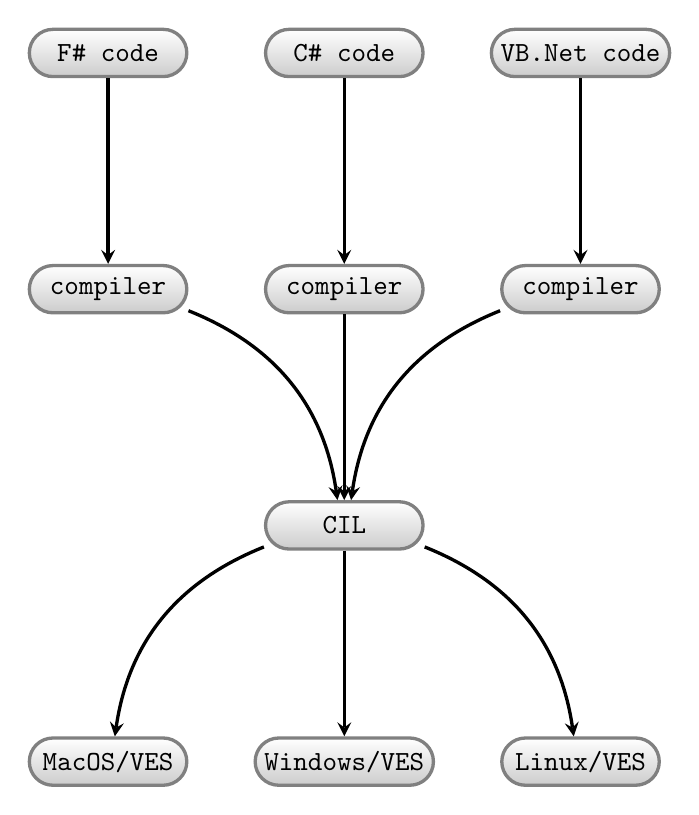
\begin{tikzpicture}[node distance=3cm,
    terminal/.style={
      % The shape:
      rectangle,minimum size=6mm,minimum width=20mm,rounded corners=3mm,
      % The rest
      very thick,draw=black!50,
      top color=white,bottom color=black!20,
      font=\ttfamily}]
    \node (fsharp)  [terminal] {F\# code};
    \node (csharp)  [terminal,right of=fsharp] {C\# code};
    \node (vb)  [terminal,right of=csharp] {VB.Net code};
    \node (fsharpc)  [terminal,below of=fsharp] {compiler}; 
    \node (csharpc)  [terminal,below of=csharp] {compiler}; 
    \node (vbc)  [terminal,below of=vb] {compiler};
    \node (cil)  [terminal,below of=csharpc] {CIL}; 
    \node (win)  [terminal,below of=cil] {Windows/VES}; 
    \node (mac)  [terminal,left of=win] {MacOS/VES}; 
    \node (lin)  [terminal,right of=win] {Linux/VES}; 
    \draw[-stealth,very thick]  (fsharp) edge (fsharpc);
    \draw[-stealth,very thick]  (csharp) edge (csharpc);
    \draw[-stealth,very thick]  (vb) edge (vbc);
    \draw[-stealth,very thick,bend left]  (fsharpc) edge (cil);
    \draw[-stealth,very thick]  (csharpc) edge (cil);
    \draw[-stealth,very thick,bend right]  (vbc) edge (cil);
    \draw[-stealth,very thick,bend right]  (cil) edge (mac);
    \draw[-stealth,very thick]  (cil) edge (win);
    \draw[-stealth,very thick,bend left]  (cil) edge (lin);
  \end{tikzpicture}
  \caption{The relation between some .NET/Mono languages with the
    Common intermediate language (CIL), and the Virtual
    execution systems (VES) on some operating system (\lstinline[language=console]{mono}).}
  \label{fig:cliOverview}
\end{figure}
First the F\# code is compiled or interpreted to CIL. This code possibly combined with other CIL code is then converted to a machine-readable code, and the result is then executed on the platform.


CLI defines a \idx{module} as a single file containing executable code by VES. Hence, CLI's notion of a module is somewhat related to F\#'s notion of module, but the two should not be confused. A collection of modules, a \idx{manifest}, and possibly other resources, which jointly define a complete program is called an \idx{assembly}. The manifest is the description of which files are included in the assembly together with its version, name, security information, and other bookkeeping information.
\end{document}


%\chapter{A brief introduction to Extended Backus-Naur Form}
\label{sec:ebnf}
\idx{Extended Backus-Naur Form} (\idx{EBNF}) is a language to specify programming languages in. The name is a tribute to John Backus who used it to describe the syntax of ALGOL58 and Peter Nauer for his work on ALGOL 60.

An EBNF consists of \idx{terminal symbols} and \idx{production rules}. Examples of typical terminal symbol are characters, numbers, punctuation marks, and whitespaces, e.g.,
\begin{lstlisting}[language=EBNF]
digit = "0" | "1" | "2" | "3" | "4" | "5" | "6" | "7" | "8" | "9" ;
\end{lstlisting}
A production rule specifies a method of combining other production rules and terminal symbols, e.g.,
\begin{lstlisting}[language=EBNF]
number = { digit } ;
\end{lstlisting}
A proposed standard for EBNF (proposal ISO/IEC 14977, \url{http://www.cl.cam.ac.uk/~mgk25/iso-14977.pdf}) is,
\begin{description}
\item '\verb|=|' definition, e.g., 
  \begin{lstlisting}[language=EBNF]
zero = "0" ;
  \end{lstlisting}
  here \verb|zero| is the terminal symbol \verb|0|.
\item '\verb|,|' concatenation, e.g.,
  \begin{lstlisting}[language=EBNF]
one = "1" ;
eleven = one, one ;
  \end{lstlisting}
  here \verb|eleven| is the terminal symbol \verb|11|.
\item '\verb|;|' termination of line
\item '\verb!|!' alternative options, e.g.,
  \begin{lstlisting}[language=EBNF]
digit = "0" | "1" | "2" | "3" | "4" | "5" | "6" | "7" | "8" | "9" ;
  \end{lstlisting}
  here \verb|digit| is the single character terminal symbol, such as \verb|3|.
\item '\verb|[ ... ]|' optional, e.g.,
  \begin{lstlisting}[language=EBNF]
zero = "0" ;
nonZeroDigit = "1" | "2" | "3" | "4" | "5" | "6" | "7" | "8" | "9" ;
nonZero = [ zero ], nonZeroDigit
  \end{lstlisting}
  here \verb|nonZero| is a non-zero digit possibly preceded by zero, such as \verb|02|.
\item '\verb|{ ... }|' repetition zero or more times, e.g., 
  \begin{lstlisting}[language=EBNF]
digit = "0" | "1" | "2" | "3" | "4" | "5" | "6" | "7" | "8" | "9" ;
number = digit, { digit }
  \end{lstlisting}
  here \verb|number| is a word consisting of 1 or more digits, such as \verb|12|.
\item '\verb|( ... )|' grouping, e.g.,
  \begin{lstlisting}[language=EBNF]
digit = "0" | "1" | "2" | "3" | "4" | "5" | "6" | "7" | "8" | "9" ;
number = digit, { digit }
expression = number, { ( "+" | "-" ), number };
  \end{lstlisting}
  here \verb|expression| is a number or a sum of numbers such as \verb|3 + 5|.
\item '\verb|" ... "|' a terminal string, e.g.,
  \begin{lstlisting}[language=EBNF]
string = "abc"' ;
  \end{lstlisting}
\item "\verb|' ... '|" a terminal string, e.g.,
  \begin{lstlisting}[language=EBNF]
string = 'abc' ;
  \end{lstlisting}
\item '\verb|(* ... *)|' a comment (* ... *) 
  \begin{lstlisting}[language=EBNF]
(* a binary digit *) digit = "0" | "1" (* from this all numbers may be constructed *) ;
  \end{lstlisting}
  Everything inside the comments are not part of the formal definition.
\item '\verb|? ... ?|' special sequence, a notation reserved for future extensions of EBNF.
\item '\verb|-|' exception, e.g.,
  \begin{lstlisting}[language=EBNF]
letter = "A" | "B" | "C" | "D" | "E" | "F" | "G" | "H" 
  | "I" | "J" | "K" | "L" | "M" | "N" | "O" | "P" | "Q" 
  | "R" | "S" | "T" | "U" | "V" | "W" | "X" | "Y" | "Z" ;
vowel = "A" | "E" | "I" | "O" | "U" ; 
consonant = letter - vowel ;
  \end{lstlisting}
  here \verb|consonant| are all letters except vowels.
\end{description}
The proposal allows for identifies that includes space, but often a reduced form is used, where identifiers are single words, in which case the concatenation symbol \verb|,| is omitted. Likewise, the termination symbol \verb|;| is often replaced with the new-line character, and if long lines must be broken, then indentation is used to signify continuation.

In this relaxed EBNF, the EBNF syntax itself can be expressed in EBNF as,
\begin{lstlisting}[language=EBNF]
letter = "A" | "B" | "C" | "D" | "E" | "F" | "G" | "H" 
  | "I" | "J" | "K" | "L" | "M" | "N" | "O" | "P" | "Q" 
  | "R" | "S" | "T" | "U" | "V" | "W" | "X" | "Y" | "Z"
  | "a" | "b" | "c" | "d" | "e" | "f" | "g" | "h" 
  | "i" | "j" | "k" | "l" | "m" | "n" | "o" | "p" | "q" 
  | "r" | "s" | "t" | "u" | "v" | "w" | "x" | "y" | "z" 
digit = "0" | "1" | "2" | "3" | "4" | "5" | "6" | "7" | "8" | "9" 
symbol = "[" | "]" | "{" | "}" | "(" | ")" | "<" | ">"
  | "'" | '"' | "=" | "|" | "." | "," | ";" 
underscore = "_" 
identifier = letter  { letter | digit | underscore } 
character = letter | digit | symbol | underscore 
string = character  { character } 
terminal = "'"  string  "'" | '"'  string  '"' 
rhs = identifier
  | terminal
  | "["  rhs  "]"
  | "{"  rhs  "}"
  | "("  rhs  ")"
  | rhs  "|"  rhs
(*  | rhs  ","  rhs  *)
rule = identifier  "="  rhs  (* ";" *)
grammar = rule { rule } 
\end{lstlisting}
Here the comments demonstrate, the relaxed modification.

%%% Local Variables:
%%% TeX-master: "fsharpNotes"
%%% End:


%\chapter{F$\flat$}
Minimal F\# used in \Cref{part:basics}
%
\lstinputlisting[language=ebnf,caption={F$\flat$, a subset of F\#},label={fflat},escapechar=§]{\src/fflat.ebnf}
%
\jon{I don't think we need \lstinline[language=ebnf]!type="'" ident! nor  \lstinline[language=ebnf]!moduleelm = "\#" ident string!}

%%% Local Variables:
%%% TeX-master: "fsharpNotes"
%%% End:


\documentclass[springer.tex]{subfiles}
\graphicspath{ {./figures/} }

\begin{document}
\chapter{Language Details}
\label{chap:details}
This appendix lists various language details.

\section{Arithmetic operators on basic types}
\begin{table}
  \centering
  \rowcolors{2}{oddRowColor}{evenRowColor}
  \begin{tabularx}{\linewidth}{|l|l|l|l|l|X|}
    \hline
    \rowcolor{headerRowColor} Operator & \lstinline!leftOp! & \lstinline!rightOp! & Expression & Result &Description\\
    \hline
    \lstinline!leftOp + rightOp!&ints & ints & \lstinline!5 + 2!&\lstinline!7!&Addition\\
             &floats & floats & \lstinline!5.0 + 2.0!&\lstinline!7.0!&\\
             &chars & chars & \lstinline!'a' + 'b'!&\lstinline!'\\195'!&Addition of codes\\
             &strings & strings & \lstinline!"ab" + "cd"!&\lstinline!"abcd"!&Concatenation\\
    \hline
    \lstinline!leftOp - rightOp!&ints & ints & \lstinline!5 - 2!&\lstinline!3!&Subtraction\\
             &floats & floats & \lstinline!5.0 - 2.0!&\lstinline!3.0!&\\
    \hline
    \lstinline!leftOp * rightOp!&ints & ints & \lstinline!5 * 2!&\lstinline!10!&Multiplication\\
             &floats & floats & \lstinline!5.0 * 2.0!&\lstinline!10.0!&\\
    \hline
    \lstinline!leftOp / rightOp!&ints & ints & \lstinline!5 / 2!&\lstinline!2!&Integer division\\
             &floats & floats & \lstinline!5.0 / 2.0!&\lstinline!2.5!&Division\\
    \hline
    \lstinline!leftOp \% rightOp!&ints & ints & \lstinline!5 \% 2!&\lstinline!1!&Remainder\\
             &floats & floats & \lstinline!5.0 \% 2.0!&\lstinline!1.0!&\\
    \hline
    \lstinline!leftOp ** rightOp!&floats & floats & \lstinline!5.0 ** 2.0!&\lstinline!25.0!&Exponentiation\\
    \hline
    \lstinline!leftOp \&\& rightOp!&bool & bool & \lstinline!true \&\& false!&\lstinline!false!&boolean and\\
    \hline
    \lstinline!leftOp || rightOp!&bool & bool & \lstinline!true || false!&\lstinline!false!&boolean or\\
    \hline
    \lstinline!leftOp \&\&\& rightOp!&ints & ints & \lstinline!0b1010 \&\&\& 0b1100!&\lstinline!0b1000!&bitwise bool and\\
    \hline
    \lstinline!leftOp ||| rightOp!&ints & ints & \lstinline!0b1010 ||| 0b1100!&\lstinline!0b1110!&bitwise boolean or\\
    \hline
    \lstinline!leftOp \^\^\^ rightOp!&ints & ints & \lstinline!0b1010 \^\^\^ 0b1101!&\lstinline!0b0111!&bitwise boolean exclusive or\\
    \hline
     \lstinline!leftOp <<< rightOp!&ints & ints & \lstinline!0b00001100uy <<< 2!&\lstinline!0b00110000uy!&bitwise shift left\\
     \hline
     \lstinline!leftOp >>> rightOp!&ints & ints & \lstinline!0b00001100uy >>> 2!&\lstinline!0b00000011uy!&bitwise and\\
     \hline
    \lstinline!+op!&ints&&\lstinline!+3!&\lstinline!3!&identity\\
             &floats&&\lstinline!+3.0!&\lstinline!3.0!&\\
    \hline
    \lstinline!-op!&ints&&\lstinline!-3!&\lstinline!-3!&negation\\
             &floats&&\lstinline!-3.0!&\lstinline!-3.0!&\\
    \hline
    \lstinline!not op!&bool&&\lstinline!not true!&\lstinline!false!&boolean negation\\
    \hline
    \lstinline!\~\~\~op!&ints&&\lstinline!\~\~\~0b00001100uy!&\lstinline!0b11110011uy!&bitwise boolean negation\\
    \hline
  \end{tabularx}
  \caption{Arithmetic operators on basic types. Ints, floats, chars, and strings means all built-in integer types etc. Note that for the bitwise operations, digits \lstinline{0} and \lstinline{1} are taken to be \lstinline{true} and \lstinline{false}.}
  \label{tab:preNInfixOperators}
\end{table}

\begin{table}
  \centering
  \rowcolors{2}{oddRowColor}{evenRowColor}
  \begin{tabularx}{\linewidth}{|l|l|l|l|l|X|}
    \hline
    \rowcolor{headerRowColor} Operator & \lstinline!leftOp! & \lstinline!rightOp! & Expression & Result &Description\\
    \hline
    \lstinline!leftOp < rightOp!&bool & bool & \lstinline!true < false!&\lstinline!false!&Less than\\
             &ints & ints & \lstinline!5 < 2!&\lstinline!false!&\\
             &floats & floats & \lstinline!5.0 < 2.0!&\lstinline!false!&\\
             &chars & chars & \lstinline!'a' < 'b'!&\lstinline!true!&\\
             &strings & strings & \lstinline!"ab" < "cd"!&\lstinline!true!&\\
    \hline
    \lstinline!leftOp > rightOp!&bool & bool & \lstinline!true > false!&\lstinline!true!&Greater than\\
             &ints & ints & \lstinline!5 > 2!&\lstinline!true!&\\
             &floats & floats & \lstinline!5.0 > 2.0!&\lstinline!true!&\\
             &chars & chars & \lstinline!'a' > 'b'!&\lstinline!false!&\\
             &strings & strings & \lstinline!"ab" > "cd"!&\lstinline!false!&\\
    \hline
    \lstinline!leftOp = rightOp!&bool & bool & \lstinline!true = false!&\lstinline!false!&Equal\\
             &ints & ints & \lstinline!5 = 2!&\lstinline!false!&\\
             &floats & floats & \lstinline!5.0 = 2.0!&\lstinline!false!&\\
             &chars & chars & \lstinline!'a' = 'b'!&\lstinline!false!&\\
             &strings & strings & \lstinline!"ab" = "cd"!&\lstinline!false!&\\
    \hline
    \lstinline!leftOp <= rightOp!&bool & bool & \lstinline!true <= false!&\lstinline!false!&Less than or equal\\
             &ints & ints & \lstinline!5 <= 2!&\lstinline!false!&\\
             &floats & floats & \lstinline!5.0 <= 2.0!&\lstinline!false!&\\
             &chars & chars & \lstinline!'a' <= 'b'!&\lstinline!true!&\\
             &strings & strings & \lstinline!"ab" <= "cd"!&\lstinline!true!&\\
    \hline
    \lstinline!leftOp >= rightOp!&bool & bool & \lstinline!true >= false!&\lstinline!true!&Greater than or equal\\
             &ints & ints & \lstinline!5 >= 2!&\lstinline!true!&\\
             &floats & floats & \lstinline!5.0 >= 2.0!&\lstinline!true!&\\
             &chars & chars & \lstinline!'a' >= 'b'!&\lstinline!false!&\\
             &strings & strings & \lstinline!"ab" >= "cd"!&\lstinline!false!&\\
    \hline
    \lstinline!leftOp <> rightOp!&bool & bool & \lstinline!true <> false!&\lstinline!true!&Not Equal\\
             &ints & ints & \lstinline!5 <> 2!&\lstinline!true!&\\
             &floats & floats & \lstinline!5.0 <> 2.0!&\lstinline!true!&\\
             &chars & chars & \lstinline!'a' <> 'b'!&\lstinline!true!&\\
             &strings & strings & \lstinline!"ab" <> "cd"!&\lstinline!true!&\\
    \hline
  \end{tabularx}
  \caption{Comparison operators on basic types. Ints, floats, chars, and strings means all built-in integer types etc..}
  \label{tab:comparisonOperators}
\end{table}
\clearpage

\section{Basic arithmetic functions}
\idxss{\lstinline{abs}}\idxss{\lstinline{acos}}\idxss{\lstinline{asin}}\idxss{\lstinline{atan}}\idxss{\lstinline{atan2}}\idxss{\lstinline{ceil}}\idxss{\lstinline{cos}}\idxss{\lstinline{cosh}}\idxss{\lstinline{exp}}\idxss{\lstinline{floor}}\idxss{\lstinline{log}}\idxss{\lstinline{log10}}\idxss{\lstinline{max}}\idxss{\lstinline{min}}\idxss{\lstinline{pown}}\idxss{\lstinline{round}}\idxss{\lstinline{sign}}\idxss{\lstinline{sin}}\idxss{\lstinline{sinh}}\idxss{\lstinline{sqrt}}\idxss{\lstinline{tan}}\idxss{\lstinline{tanh}}
\begin{table}
  \centering
  \rowcolors{2}{oddRowColor}{evenRowColor}
  \begin{tabular}{|l|l|l|l|l|}
    \hline
    \rowcolor{headerRowColor} Type & Function name & Example & Result & Description\\
    \hline
    Ints and floats & \lstinline!abs! & \lstinline!abs -3! & \lstinline!3! & Absolute value\\
    \hline 
    Floats & \lstinline!acos! & \lstinline!acos 0.8! & \lstinline!0.6435011088! & Inverse cosine\\
    \hline 
    Floats & \lstinline!asin! & \lstinline!asin 0.8! & \lstinline!0.927295218! & Inverse sinus\\
    \hline 
    Floats & \lstinline!atan! & \lstinline!atan 0.8! & \lstinline!0.6747409422! & Inverse tangent\\
    \hline 
    Floats & \lstinline!atan2! & \lstinline!atan2 0.8 2.3! & \lstinline!0.3347368373! & Inverse tangentvariant\\
    \hline 
    Floats & \lstinline!ceil! & \lstinline!ceil 0.8! & \lstinline!1.0! & Ceiling\\
    \hline 
    Floats & \lstinline!cos! & \lstinline!cos 0.8! & \lstinline!0.6967067093! & Cosine\\
    \hline 
    Floats & \lstinline!cosh! & \lstinline!cosh 0.8! & \lstinline!1.337434946! & Hyperbolic cosine\\
    \hline 
    Floats & \lstinline!exp! & \lstinline!exp 0.8! & \lstinline!2.225540928! & Natural exponent\\
    \hline 
    Floats & \lstinline!floor! & \lstinline!floor 0.8! & \lstinline!0.0! & Floor\\
    \hline 
    Floats & \lstinline!log! & \lstinline!log 0.8! & \lstinline!-0.2231435513! & Natural logarithm\\
    \hline 
    Floats & \lstinline!log10! & \lstinline!log10 0.8! & \lstinline!-0.09691001301! & Base-10 logarithm\\
    \hline 
    \begin{minipage}[t]{0.175\linewidth}Ints, floats,\\chars, and strings\end{minipage} & \lstinline!max! & \lstinline!max 3.0 4.0! & \lstinline!4.0! & Maximum\\
    \hline 
    \begin{minipage}[t]{0.175\linewidth}Ints, floats,\\chars, and strings\end{minipage} & \lstinline!min! & \lstinline!min 3.0 4.0! & \lstinline!3.0! & Minimum\\
    \hline 
    Ints & \lstinline!pown! & \lstinline!pown 3 2! & \lstinline!9! & Integer exponent\\
    \hline 
    Floats & \lstinline!round! & \lstinline!round 0.8! & \lstinline!1.0! & Rounding\\
    \hline 
    Ints and floats & \lstinline!sign! & \lstinline!sign -3! & \lstinline!-1! & Sign\\
    \hline 
    Floats & \lstinline!sin! & \lstinline!sin 0.8! & \lstinline!0.7173560909! & Sinus\\
    \hline 
    Floats & \lstinline!sinh! & \lstinline!sinh 0.8! & \lstinline!0.8881059822! & Hyperbolic sinus\\
    \hline 
    Floats & \lstinline!sqrt! & \lstinline!sqrt 0.8! & \lstinline!0.894427191! & Square root\\
    \hline 
    Floats & \lstinline!tan! & \lstinline!tan 0.8! & \lstinline!1.029638557! & Tangent\\
    \hline 
    Floats & \lstinline!tanh! & \lstinline!tanh 0.8! & \lstinline!0.6640367703! & Hyperbolic tangent\\
    \hline 
  \end{tabular}
  \caption{Predefined functions for arithmetic operations}
  \label{tab:arithmeticFunctions}
\end{table}

\begin{table}
  \centering
  \begin{tabularx}{\linewidth}{|l|l|X|}
    \hline
    Name& Example & Description\\
    \hline
    \lstinline{fst} & \lstinline{fst (1, 2)} &\\
    \hline
    \lstinline{snd} & \lstinline{snd (1, 2)} &\\
    \hline
    \lstinline{failwith} & \lstinline{failwith} &\\
    \hline
    \lstinline{invalidArg} & \lstinline{invalidArg} &\\
    \hline
    \lstinline{raise} & \lstinline{raise} &\\
    \hline
    \lstinline{reraise} & \lstinline{reraise} &\\
    \hline
    \lstinline{ref} & \lstinline{ref} &\\
    \hline
%    \lstinline|(!)| & \lstinline|!| &\\
    \hline
    \lstinline{ceil} & \lstinline{ceil} &\\
    \hline
  \end{tabularx}
  \caption{Built-in functions.}
  \label{tab:simpleBuiltInFct}
\end{table}
\clearpage

\section{Precedence and associativity}
\begin{comment}
\begin{table}
  \centering
  \rowcolors{2}{oddRowColor}{evenRowColor}
  \begin{tabularx}{\linewidth}{|>{\hsize=.8\hsize\raggedright\arraybackslash}X|>{\hsize=.4\hsize}X|>{\hsize=1.8\hsize}X|}
    \hline
    \rowcolor{headerRowColor}     Operator & Associativity & Description\\
    \hline
    \mbox{\lstinline|+op|,} \mbox{\lstinline|-op|,} \mbox{\lstinline|\~\~\~op|} & Left & Unary identity, negation, and bitwise negation operator\\
    \hline
    \lstinline|f x| & Left & Function application\\
    \hline
    \lstinline|leftOp ** rightOp| & Right & Exponent\\ 
    \hline
    \mbox{\lstinline|leftOp * rightOp|,} \mbox{\lstinline|leftOp / rightOp|,} \mbox{\lstinline|leftOp \% rightOp|} & Left & Multiplication, division and remainder\\
    \hline
    \mbox{\lstinline|leftOp + rightOp|,} \mbox{\lstinline|leftOp - rightOp|} & Left & Addition and subtraction binary operators\\
    \hline
    \lstinline|leftOp \^\^\^ rightOp| & Right & bitwise exclusive or\\
    \hline
    \mbox{\lstinline|leftOp < rightOp|,} \mbox{\lstinline|leftOp <= rightOp|,} \mbox{\lstinline|leftOp > rightOp|,} \mbox{\lstinline|leftOp >= rightOp|,} \mbox{\lstinline|leftOp = rightOp|,} \mbox{\lstinline|leftOp <> rightOp|,} \mbox{\lstinline|leftOp <<< rightOp|,} \mbox{\lstinline|leftOp >>> rightOp|,} \mbox{\lstinline|leftOp \&\&\& rightOp|,} \mbox{\lstinline!leftOp ||| rightOp!,}
             & Left & Comparison operators, bitwise shift, and bitwise 'and' and 'or'.\\
    \hline
    \lstinline|\&\&| & Left & Boolean and\\
    \hline
    \lstinline+||+ & Left & Boolean or\\
    \hline
  \end{tabularx}
  \caption{Some common operators, their precedence, and their associativity. Rows are ordered from highest to lowest precedences, such that \lstinline|leftOp * rightOp| has higher precedence than \lstinline|leftOp + rightOp|. Operators in the same row has same precedence. Full table is given in \Cref{tab:operatorPrecedence}.}
  \label{tab:someOperatorPrecedences}
\end{table}
\end{comment}

\idxs{boolean or}\idxs{boolean and}
\begin{table}
  \centering
  \begin{tabularx}{\linewidth}{|>{\hsize=1\hsize\raggedright\arraybackslash}X|>{\hsize=.5\hsize}X|>{\hsize=1.5\hsize}X|}
    \hline
    Operator & Associativity & Description\\
    \hline
    \lstinline[language=ebnf]|ident "<" types ">"| & Left & High-precedence type application\\
    \hline
    \lstinline[language=ebnf]|ident "(" expr ")"| & Left & High-predence application\\
    \hline
    \lstinline[language=ebnf]|"."| & Left & \\
    \hline
    \lstinline[language=ebnf]|prefixOp| & Left & All prefix operators\\
    \hline
    \lstinline[language=ebnf]|"|" rule| & Left & Pattern matching rule\\
    \hline
    \mbox{\lstinline[language=ebnf]|ident expr|,} \mbox{\lstinline[language=ebnf]|"lazy'' expr|,} \mbox{\lstinline[language=ebnf]|"assert'' epxr|} & Left & \\
    \hline
    \lstinline[language=ebnf]|"**" {opChar}| & Right & Exponent like\\
    \hline
    \mbox{\lstinline[language=ebnf]|"*"  {opChar}|,} \mbox{\lstinline[language=ebnf]|"/"  {opChar}|,} \mbox{\lstinline[language=ebnf]|"\%"  {opChar}|} & Left & Infix multiplication like\\
     \hline
    \mbox{\lstinline[language=ebnf]|"-"  {opChar}|,} \mbox{\lstinline[language=ebnf]|"+"  {opChar}|} & Left & Infix addition like\\
     \hline
     \lstinline[language=ebnf]|":?''| & None & \\
     \hline
     \lstinline[language=ebnf]|"::''| & Right & \\
     \hline
     \lstinline[language=ebnf]|"^''  {opChar}| & Right & \\
     \hline
    \mbox{\lstinline[language=ebnf]|"!="  {opChar}|,} \mbox{\lstinline[language=ebnf]|"<"  {opChar}|,} \mbox{\lstinline[language=ebnf]|">"  {opChar}|,} \mbox{\lstinline[language=ebnf]|"="|,} \mbox{\lstinline[language=ebnf]!"|"  {opChar}!,} \mbox{\lstinline[language=ebnf]|"\&"  {opChar}|,} \mbox{\lstinline[language=ebnf]|"\$"  {opChar}|} & Left & Infix addition like\\
     \hline
    \mbox{\lstinline[language=ebnf]|":>"|,} \mbox{\lstinline[language=ebnf]|":?>"|} & Right & \\
     \hline
    \mbox{\lstinline[language=ebnf]|"\&"|,} \mbox{\lstinline[language=ebnf]|"\&\&"|} & Left & Boolean and like\\
     \hline
    \mbox{\lstinline[language=ebnf]|"or"|,} \mbox{\lstinline[language=ebnf]!"||"!} & Left & Boolean or like\\
     \hline
     \lstinline[language=ebnf]|","| & None & \\
     \hline
     \lstinline[language=ebnf]|":="| & Right & \\
     \hline
     \lstinline[language=ebnf]|"->"| & Right & \\
     \hline
    \lstinline[language=ebnf]|"if"| & None & \\
     \hline
    \mbox{\lstinline[language=ebnf]|"function"|,} \mbox{\lstinline[language=ebnf]|"fun"|,} \mbox{\lstinline[language=ebnf]|"match"|,} \mbox{\lstinline[language=ebnf]|"try"|}& None & \\
     \hline
     \lstinline[language=ebnf]|"let"| & None & \\
     \hline
     \lstinline[language=ebnf]|";"| & Right & \\
     \hline
     \lstinline[language=ebnf]!"|"! & Left & \\
     \hline
     \lstinline[language=ebnf]|"when"| & Right & \\
     \hline
     \lstinline[language=ebnf]|"as"| & Right & \\
     \hline
  \end{tabularx}
  \caption{Precedence and associativity of operators. Operators in the same row has same precedence. See \Cref{list:infixOrPrefixOperators} for the definition of \lstinline!prefixOp!}
  \label{tab:operatorPrecedence}
\end{table}
\clearpage

\begin{comment}
\section{Behind the scene}
\jon{I'm not sure, whether it will be a good idea to describe this. Could be used as the umbrella for the specification of the program.} When a program is compiled or interpreted the following steps are performed by the system
  \begin{enumerate}
  \item Decoding
  \item Tokenization
  \item Lexical Filtering
  \item Parsing
  \item Importing
  \item Checking
  \item Elaboration
  \item Execution
  \end{enumerate}
  \dots
\end{comment}

%\section{Lightweight Syntax}
%To appear later.\jon{See Lightweight Syntax, Spec-4.0 Chapter 15.1}
\end{document}
%%% Local Variables:
%%% TeX-master: "fsharpNotes"
%%% End:



%\documentclass[springer.tex]{subfiles}
\graphicspath{ {./figures/} }

\begin{document}
\chapter{The Some Basic Libraries}
\label{chap:collection}
\jon{Work in progress!}

\jon{Discuss \lstinline{Fsharp.Core} and \lstinline{System} and all the operators and functions defined there.}
\jon{See \url{https://msdn.microsoft.com/en-us/visualfsharpdocs/conceptual/import-declarations-the-open-keyword-fsharp} for namespaces opened per default.}

\section{\lstinline{System.String}}
\label{sec:system.string}
The list of built-in methods accessible with the dot notation is defined in \lstinline|System.String| class and is long. Here follow short descriptions of some useful methods:
\begin{description}
%\item[\lstinline{Clone}] Returns a reference to this instance of String.
\item[\lstinline{Compare(String, String)}] Compares two specified String objects and returns an integer that indicates their relative position in the sort order.
%\item[\lstinline{Compare(String, String, Boolean)}] Compares two specified String objects, ignoring or honoring their case, and returns an integer that indicates their relative position in the sort order.
%\item[\lstinline{Compare(String, String, StringComparison)}] Compares two specified String objects using the specified rules, and returns an integer that indicates their relative position in the sort order.
%\item[\lstinline{Compare(String, String, Boolean, CultureInfo)}] Compares two specified String objects, ignoring or honoring their case, and using culture-specific information to influence the comparison, and returns an integer that indicates their relative position in the sort order.
%\item[\lstinline{Compare(String, String, CultureInfo, CompareOptions)}] Compares two specified String objects using the specified comparison options and culture-specific information to influence the comparison, and returns an integer that indicates the relationship of the two strings to each other in the sort order.
%\item[\lstinline{Compare(String, Int32, String, Int32, Int32)}] Compares substrings of two specified String objects and returns an integer that indicates their relative position in the sort order.
%\item[\lstinline{Compare(String, Int32, String, Int32, Int32, Boolean)}] Compares substrings of two specified String objects, ignoring or honoring their case, and returns an integer that indicates their relative position in the sort order.
%\item[\lstinline{Compare(String, Int32, String, Int32, Int32, StringComparison)}] Compares substrings of two specified String objects using the specified rules, and returns an integer that indicates their relative position in the sort order.
%\item[\lstinline{Compare(String, Int32, String, Int32, Int32, Boolean, CultureInfo)}] Compares substrings of two specified String objects, ignoring or honoring their case and using culture-specific information to influence the comparison, and returns an integer that indicates their relative position in the sort order.
%\item[\lstinline{Compare(String, Int32, String, Int32, Int32, CultureInfo, CompareOptions)}] Compares substrings of two specified String objects using the specified comparison options and culture-specific information to influence the comparison, and returns an integer that indicates the relationship of the two substrings to each other in the sort order.
\item[\lstinline{CompareOrdinal(String, String)}] Compares two specified String objects by evaluating the numeric values of the corresponding Char objects in each string.
\item[\lstinline{CompareOrdinal(String, Int32, String, Int32, Int32)}] Compares substrings of two specified String objects by evaluating the numeric values of the corresponding Char objects in each substring.
\item[\lstinline{CompareTo(Object)}] Compares this instance with a specified Object and indicates whether this instance precedes, follows, or appears in the same position in the sort order as the specified Object.
\item[\lstinline{CompareTo(String)}] Compares this instance with a specified String object and indicates whether this instance precedes, follows, or appears in the same position in the sort order as the specified String.
\item[\lstinline{Concat(Object)}] Creates the string representation of a specified object.
\item[\lstinline{Concat(Object[])}] Concatenates the string representations of the elements in a specified Object array.
\item[\lstinline{Concat(IEnumerable(String))}] Concatenates the members of a constructed IEnumerable(T) collection of type String.
\item[\lstinline{Concat(String[])}] Concatenates the elements of a specified String array.
\item[\lstinline{Concat(Object, Object)}] Concatenates the string representations of two specified objects.
\item[\lstinline{Concat(String, String)}] Concatenates two specified instances of String.
\item[\lstinline{Concat(Object, Object, Object)}] Concatenates the string representations of three specified objects.
\item[\lstinline{Concat(String, String, String)}] Concatenates three specified instances of String.
\item[\lstinline{Concat(Object, Object, Object, Object)}] Concatenates the string representations of four specified objects and any objects specified in an optional variable length parameter list.
\item[\lstinline{Concat(String, String, String, String)}] Concatenates four specified instances of String.
\item[\lstinline{Concat(T)(IEnumerable(T))}] Concatenates the members of an IEnumerable(T) implementation.
\item[\lstinline{Contains}] Returns a value indicating whether the specified String object occurs within this string.
\item[\lstinline{Copy}] Creates a new instance of String with the same value as a specified String.
\item[\lstinline{CopyTo}] Copies a specified number of characters from a specified position in this instance to a specified position in an array of Unicode characters.
\item[\lstinline{EndsWith(String)}] Determines whether the end of this string instance matches the specified string.
\item[\lstinline{EndsWith(String, StringComparison)}] Determines whether the end of this string instance matches the specified string when compared using the specified comparison option.
\item[\lstinline{EndsWith(String, Boolean, CultureInfo)}] Determines whether the end of this string instance matches the specified string when compared using the specified culture.
\item[\lstinline{Equals(Object)}] Determines whether this instance and a specified object, which must also be a String object, have the same value. (Overrides Object.Equals(Object).)
\item[\lstinline{Equals(String)}] Determines whether this instance and another specified String object have the same value.
\item[\lstinline{Equals(String, String)}] Determines whether two specified String objects have the same value.
\item[\lstinline{Equals(String, StringComparison)}] Determines whether this string and a specified String object have the same value. A parameter specifies the culture, case, and sort rules used in the comparison.
\item[\lstinline{Equals(String, String, StringComparison)}] Determines whether two specified String objects have the same value. A parameter specifies the culture, case, and sort rules used in the comparison.
\item[\lstinline{Finalize}] Allows an object to try to free resources and perform other cleanup operations before it is reclaimed by garbage collection. (Inherited from Object.)
\item[\lstinline{Format(String, Object)}] Replaces one or more format items in a specified string with the string representation of a specified object.
\item[\lstinline{Format(String, Object[])}] Replaces the format item in a specified string with the string representation of a corresponding object in a specified array.
\item[\lstinline{Format(IFormatProvider, String, Object[])}] Replaces the format item in a specified string with the string representation of a corresponding object in a specified array. A specified parameter supplies culture-specific formatting information.
\item[\lstinline{Format(String, Object, Object)}] Replaces the format items in a specified string with the string representation of two specified objects.
\item[\lstinline{Format(String, Object, Object, Object)}] Replaces the format items in a specified string with the string representation of three specified objects.
\item[\lstinline{GetEnumerator}] Retrieves an object that can iterate through the individual characters in this string.
\item[\lstinline{GetHashCode}] Returns the hash code for this string. (Overrides Object.GetHashCode().)
\item[\lstinline{GetType}] Gets the Type of the current instance. (Inherited from Object.)
\item[\lstinline{GetTypeCode}] Returns the TypeCode for class String.
\item[\lstinline{IndexOf(Char)}] Reports the zero-based index of the first occurrence of the specified Unicode character in this string.
\item[\lstinline{IndexOf(String)}] Reports the zero-based index of the first occurrence of the specified string in this instance.
\item[\lstinline{IndexOf(Char, Int32)}] Reports the zero-based index of the first occurrence of the specified Unicode character in this string. The search starts at a specified character position.
\item[\lstinline{IndexOf(String, Int32)}] Reports the zero-based index of the first occurrence of the specified string in this instance. The search starts at a specified character position.
\item[\lstinline{IndexOf(String, StringComparison)}] Reports the zero-based index of the first occurrence of the specified string in the current String object. A parameter specifies the type of search to use for the specified string.
\item[\lstinline{IndexOf(Char, Int32, Int32)}] Reports the zero-based index of the first occurrence of the specified character in this instance. The search starts at a specified character position and examines a specified number of character positions.
\item[\lstinline{IndexOf(String, Int32, Int32)}] Reports the zero-based index of the first occurrence of the specified string in this instance. The search starts at a specified character position and examines a specified number of character positions.
\item[\lstinline{IndexOf(String, Int32, StringComparison)}] Reports the zero-based index of the first occurrence of the specified string in the current String object. Parameters specify the starting search position in the current string and the type of search to use for the specified string.
\item[\lstinline{IndexOf(String, Int32, Int32, StringComparison)}] Reports the zero-based index of the first occurrence of the specified string in the current String object. Parameters specify the starting search position in the current string, the number of characters in the current string to search, and the type of search to use for the specified string.
\item[\lstinline{IndexOfAny(Char[])}] Reports the zero-based index of the first occurrence in this instance of any character in a specified array of Unicode characters.
\item[\lstinline{IndexOfAny(Char[], Int32)}] Reports the zero-based index of the first occurrence in this instance of any character in a specified array of Unicode characters. The search starts at a specified character position.
\item[\lstinline{IndexOfAny(Char[], Int32, Int32)}] Reports the zero-based index of the first occurrence in this instance of any character in a specified array of Unicode characters. The search starts at a specified character position and examines a specified number of character positions.
\item[\lstinline{Insert}] Returns a new string in which a specified string is inserted at a specified index position in this instance.
\item[\lstinline{Intern}] Retrieves the system's reference to the specified String.
\item[\lstinline{IsInterned}] Retrieves a reference to a specified String.
\item[\lstinline{IsNormalized()}] Indicates whether this string is in Unicode normalization form C.
\item[\lstinline{IsNormalized(NormalizationForm)}] Indicates whether this string is in the specified Unicode normalization form.
\item[\lstinline{IsNullOrEmpty}] Indicates whether the specified string is a null reference (Nothing in Visual Basic) or an Empty string.
\item[\lstinline{IsNullOrWhiteSpace}] Indicates whether a specified string is a null reference (Nothing in Visual Basic), empty, or consists only of whitespace characters.
\item[\lstinline{Join(String, IEnumerable(String))}] Concatenates the members of a constructed IEnumerable(T) collection of type String, using the specified separator between each member.
\item[\lstinline{Join(String, Object[])}] Concatenates the elements of an object array, using the specified separator between each element.
\item[\lstinline{Join(String, String[])}] Concatenates all the elements of a string array, using the specified separator between each element.
\item[\lstinline{Join(String, String[], Int32, Int32)}] Concatenates the specified elements of a string array, using the specified separator between each element.
\item[\lstinline{Join(T)(String, IEnumerable(T))}] Concatenates the members of a collection, using the specified separator between each member.
\item[\lstinline{LastIndexOf(Char)}] Reports the zero-based index position of the last occurrence of a specified Unicode character within this instance.
\item[\lstinline{LastIndexOf(String)}] Reports the zero-based index position of the last occurrence of a specified string within this instance.
\item[\lstinline{LastIndexOf(Char, Int32)}] Reports the zero-based index position of the last occurrence of a specified Unicode character within this instance. The search starts at a specified character position.
\item[\lstinline{LastIndexOf(String, Int32)}] Reports the zero-based index position of the last occurrence of a specified string within this instance. The search starts at a specified character position.
\item[\lstinline{LastIndexOf(String, StringComparison)}] Reports the zero-based index of the last occurrence of a specified string within the current String object. A parameter specifies the type of search to use for the specified string.
\item[\lstinline{LastIndexOf(Char, Int32, Int32)}] Reports the zero-based index position of the last occurrence of the specified Unicode character in a substring within this instance. The search starts at a specified character position and examines a specified number of character positions.
\item[\lstinline{LastIndexOf(String, Int32, Int32)}] Reports the zero-based index position of the last occurrence of a specified string within this instance. The search starts at a specified character position and examines a specified number of character positions.
\item[\lstinline{LastIndexOf(String, Int32, StringComparison)}] Reports the zero-based index of the last occurrence of a specified string within the current String object. Parameters specify the starting search position in the current string, and type of search to use for the specified string.
\item[\lstinline{LastIndexOf(String, Int32, Int32, StringComparison)}] Reports the zero-based index position of the last occurrence of a specified string within this instance. Parameters specify the starting search position in the current string, the number of characters in the current string to search, and the type of search to use for the specified string.
\item[\lstinline{LastIndexOfAny(Char[])}] Reports the zero-based index position of the last occurrence in this instance of one or more characters specified in a Unicode array.
\item[\lstinline{LastIndexOfAny(Char[], Int32)}] Reports the zero-based index position of the last occurrence in this instance of one or more characters specified in a Unicode array. The search starts at a specified character position.
\item[\lstinline{LastIndexOfAny(Char[], Int32, Int32)}] Reports the zero-based index position of the last occurrence in this instance of one or more characters specified in a Unicode array. The search starts at a specified character position and examines a specified number of character positions.
\item[\lstinline{MemberwiseClone}] Creates a shallow copy of the current Object. (Inherited from Object.)
\item[\lstinline{Normalize()}] Returns a new string whose textual value is the same as this string, but whose binary representation is in Unicode normalization form C.
\item[\lstinline{Normalize(NormalizationForm)}] Returns a new string whose textual value is the same as this string, but whose binary representation is in the specified Unicode normalization form.
\item[\lstinline{PadLeft(Int32)}] Returns a new string that right-aligns the characters in this instance by padding them with spaces on the left, for a specified total length.
\item[\lstinline{PadLeft(Int32, Char)}] Returns a new string that right-aligns the characters in this instance by padding them on the left with a specified Unicode character, for a specified total length.
\item[\lstinline{PadRight(Int32)}] Returns a new string that left-aligns the characters in this string by padding them with spaces on the right, for a specified total length.
\item[\lstinline{PadRight(Int32, Char)}] Returns a new string that left-aligns the characters in this string by padding them on the right with a specified Unicode character, for a specified total length.
\item[\lstinline{Remove(Int32)}] Returns a new string in which all the characters in the current instance, beginning at a specified position and continuing through the last position, have been deleted.
\item[\lstinline{Remove(Int32, Int32)}] Returns a new string in which a specified number of characters in this instance beginning at a specified position have been deleted.
\item[\lstinline{Replace(Char, Char)}] Returns a new string in which all occurrences of a specified Unicode character in this instance are replaced with another specified Unicode character.
\item[\lstinline{Replace(String, String)}] Returns a new string in which all occurrences of a specified string in the current instance are replaced with another specified string.
\item[\lstinline{Split(Char[])}] Returns a string array that contains the substrings in this instance that are delimited by elements of a specified Unicode character array.
\item[\lstinline{Split(Char[], Int32)}] Returns a string array that contains the substrings in this instance that are delimited by elements of a specified Unicode character array. A parameter specifies the maximum number of substrings to return.
\item[\lstinline{Split(Char[], StringSplitOptions)}] Returns a string array that contains the substrings in this string that are delimited by elements of a specified Unicode character array. A parameter specifies whether to return empty array elements.
\item[\lstinline{Split(String[], StringSplitOptions)}] Returns a string array that contains the substrings in this string that are delimited by elements of a specified string array. A parameter specifies whether to return empty array elements.
\item[\lstinline{Split(Char[], Int32, StringSplitOptions)}] Returns a string array that contains the substrings in this string that are delimited by elements of a specified Unicode character array. Parameters specify the maximum number of substrings to return and whether to return empty array elements.
\item[\lstinline{Split(String[], Int32, StringSplitOptions)}] Returns a string array that contains the substrings in this string that are delimited by elements of a specified string array. Parameters specify the maximum number of substrings to return and whether to return empty array elements.
\item[\lstinline{StartsWith(String)}] Determines whether the beginning of this string instance matches the specified string.
\item[\lstinline{StartsWith(String, StringComparison)}] Determines whether the beginning of this string instance matches the specified string when compared using the specified comparison option.
\item[\lstinline{StartsWith(String, Boolean, CultureInfo)}] Determines whether the beginning of this string instance matches the specified string when compared using the specified culture.
\item[\lstinline{Substring(Int32)}] Retrieves a substring from this instance. The substring starts at a specified character position.
\item[\lstinline{Substring(Int32, Int32)}] Retrieves a substring from this instance. The substring starts at a specified character position and has a specified length.
\item[\lstinline{ToCharArray()}] Copies the characters in this instance to a Unicode character array.
\item[\lstinline{ToCharArray(Int32, Int32)}] Copies the characters in a specified substring in this instance to a Unicode character array.
\item[\lstinline{ToLower()}] Returns a copy of this string converted to lowercase.
\item[\lstinline{ToLower(CultureInfo)}] Returns a copy of this string converted to lowercase, using the casing rules of the specified culture.
\item[\lstinline{ToLowerInvariant}] Returns a copy of this String object converted to lowercase using the casing rules of the invariant culture.
\item[\lstinline{ToString()}] Returns this instance of String; no actual conversion is performed. (Overrides Object.ToString().)
\item[\lstinline{ToString(IFormatProvider)}] Returns this instance of String; no actual conversion is performed.
\item[\lstinline{ToUpper()}] Returns a copy of this string converted to uppercase.
\item[\lstinline{ToUpper(CultureInfo)}] Returns a copy of this string converted to uppercase, using the casing rules of the specified culture.
\item[\lstinline{ToUpperInvariant}] Returns a copy of this String object converted to uppercase using the casing rules of the invariant culture.
\item[\lstinline{Trim()}] Removes all leading and trailing whitespace characters from the current String object.
\item[\lstinline{Trim(Char[])}] Removes all leading and trailing occurrences of a set of characters specified in an array from the current String object.
\item[\lstinline{TrimEnd}] Removes all trailing occurrences of a set of characters specified in an array from the current String object.
\item[\lstinline{TrimStart}] Removes all leading occurrences of a set of characters specified in an array from the current String object.
\end{description}


\section{WinForms Details}

\begin{table}
  \begin{center}
  \rowcolors{2}{oddRowColor}{evenRowColor}
    \begin{tabularx}{\linewidth}{|l|X|}
      \hline
      \rowcolor{headerRowColor}  Function & Description\\
      \hline
      \lstinline{DataGridView}
      &Display data on a table.\\
      \hline
      \lstinline{TextBox}
      &Display editable text.\\
      \hline
      \lstinline{Label}
      &Display text.\\
      \hline
      \lstinline{LinkLabel}
      &Display clickable text.\\
      \hline
      \lstinline{ProgressBar}
      &Display the current progress as a bar.\\
      \hline
      \lstinline{WebBrwoser}
      &Enable navigation of the web.\\
      \hline
      \lstinline{CheckedListBox}
      &Display a scrollable check box list.\\
      \hline
      \lstinline{ComboBox}
      &Display a drop-down list.\\
      \hline
      \lstinline{ListBox}
      &Display a list of text and icons.\\
      \hline
      \lstinline{PictureBox}
      &Display a bitmap image\\
      \hline
      \lstinline{CheckBox}
      &Display a checkbox and a label of text.\\
      \hline
      \lstinline{RadioButton}
      &Display an on-off radio button\\
      \hline
      \lstinline{TrackBar}
      &Enable the user to input value by moving a cursor on a slider bar\\
      \hline
      \lstinline{DateTimePicker}
      &Enable the user to select a date from a graphical calendar\\
      \hline
      \lstinline{ColorDialogue}
      &Enable the user to pick a color\\
      \hline
      \lstinline{FontDialog}
      &Enable the user to pick a font and its attributes\\
      \hline
      \lstinline{OpenFileDialog}
      &Enable the user to navigate the file system and select a file..\\
      \hline
      \lstinline{PrintDialog}
      &Enable the user to select a printer and its attributes.\\
      \hline
      \lstinline{SaveDialog}
      &Enable the user to navigate the file system and specify a filename.\\
      \hline
      \lstinline{MenuStrip}
      &Allow the user to choose from a custom menu\\
      \hline
      \lstinline{Button}
      &Display a clickable button with text\\
      \hline
      \lstinline{Tooltip}
      &Briefly display a pop-up window, when the user rests the pointer on the control\\
      \hline
      \lstinline{SoundPlayer}
      &Play sounds in the \lstinline{.wav} format.\\
      \hline
    \end{tabularx}
  \end{center}
  \caption{Some controls available in WinForms.}
  \label{tab:controls}
\end{table}

\begin{table}
  \begin{center}
  \rowcolors{2}{oddRowColor}{evenRowColor}
    \begin{tabularx}{\linewidth}{|l|X|}
      \hline
      \rowcolor{headerRowColor}  Function & Description\\
      \hline
      \lstinline{Panel}
      &Groups a set of controls in a scrollable frame.\\
      \hline
      \lstinline{GroupBox}
      &Group a set of controls in a non-scrollable frame.\\
      \hline
      \lstinline{TabControl}
      &Group controls in tabpages, A tabpage is selected by clicking on its tab.\\
      \hline
      \lstinline{SplitContainer}
      &Group controls into two resizable panels.\\
      \hline
      \lstinline{TableLayoutPanel}
      &Group controls into a grid.\\
      \hline
      \lstinline{FlowLayoutPanel}
      &Group controls into a set of flowable panels. The panels may flow horizontally or vertically as a response to window resizing.\\
      \hline
    \end{tabularx}
  \end{center}
  \caption{Some controls for grouping other controls.}
  \label{tab:controlGroups}
\end{table}

\dots

\section{Mutable Collections}
\lstinline[language=console]|System.Collections.Generic|
\subsection{Mutable lists}
\lstinline[language=console]|List|,  \lstinline[language=console]|LinkedList|
\subsection{Stacks}
\lstinline[language=console]|Stack|
\subsection{Queues}  
\lstinline[language=console]|Queue|
\subsection{Sets and dictionaries}
\lstinline[language=console]|HashSet|,  and \lstinline[language=console]|Dictionary| from  
\end{document}
%%% Local Variables:
%%% TeX-master: "fsharpNotes"
%%% End:



\documentclass[fsharpNotes.tex]{subfiles}
\graphicspath{ {./figures/} }

\begin{document}
\chapter{To Do}
\begin{itemize}
\item Make sure \lstinline{#quit;;} or \texttt{ctrl-d} is included in the first chapters
\end{itemize}
\chapter{Old To Dos}
\begin{itemize}
\item Go through all idxss and make sure they should not be in the
  margin.
\item Figure out a consistent way to handle System... in the margin
  and index.
\item Integrate language details into main text.
\item Add Winforms Bitmap (and fillable objects)
\item Add Winforms Refresh
\item Add appendix on regular expressions
\item Add Torben's notes on functional programming
\item Add a chapter comparing the 3 paradigms
\item Add abstraction of computer: places <-> memory/disk. Mutable objects are abstractions of places \url{https://www.infoq.com/presentations/Value-Values}. Facts does not rime with set and get. 
\item Hickey: Difference between syntax and semantics. Values or locations, add a good figure. Functional programming: All values are freely shareable.
\item something about organizing stuff: \url{https://fsharpforfunandprofit.com/posts/organizing-functions/}, \url{https://fsharpforfunandprofit.com/posts/recipe-part3/}
\item why discriminant unions and function overloading is problematic: \url{http://stefanalfbo.github.io/blog/2014/01/05/fsharp-function-overloading/}
\item Maybe something from \url{https://fsharpforfunandprofit.com/posts/type-extensions/}
\item Maybe publish with \url{https://www.lulu.com}
\item consider following convention \url{http://fsprojects.github.io/FSharpLint/NameConventions.html},  particularly PascalCase instead of camelCase.
\item Somewhere describe generic functions and type definitions
\item Credit to Hans for early version of Console chapter.
\item Possible highlight changes in code stumps, and possibly improve reference to code used for each compilation example.
\item Railway oriented programming \url{https://fsharpforfunandprofit.com/rop/}
\item Reference and value discussion in listable things.
\item Possibly an overview table of reference and value types.
\item Some possible oop examples \url{https://www3.ntu.edu.sg/home/ehchua/programming/cpp/cp5_OOPExamples.html}
\item Should boxing be mentioned? \lstinline|(box 5) :?> int;;|, see Spec-4.0 chapter 18.2.6.
\item In object-oriented programming: functions and data are combined. Contrast the Anemic Domain Model (\url{https://www.martinfowler.com/bliki/AnemicDomainModel.html})
\item boxing \lstinline|(box 5) :?> int;;|, see Spec-4.0 chapter 18.2.6.
\end{itemize}
\end{document}
%%% Local Variables:
%%% TeX-master: "fsharpNotes"
%%% End:



\clearpage
\addcontentsline{toc}{chapter}{Bibliography}
\bibliographystyle{plain}
\bibliography{references}

\clearpage
\addcontentsline{toc}{chapter}{Index}
\printindex

\end{document}
